\documentclass[twoside]{book}

% Packages required by doxygen
\usepackage{fixltx2e}
\usepackage{calc}
\usepackage{doxygen}
\usepackage[export]{adjustbox} % also loads graphicx
\usepackage{graphicx}
\usepackage[utf8]{inputenc}
\usepackage{makeidx}
\usepackage{multicol}
\usepackage{multirow}
\PassOptionsToPackage{warn}{textcomp}
\usepackage{textcomp}
\usepackage[nointegrals]{wasysym}
\usepackage[table]{xcolor}

% Font selection
\usepackage[T1]{fontenc}
\usepackage[scaled=.90]{helvet}
\usepackage{courier}
\usepackage{amssymb}
\usepackage{sectsty}
\renewcommand{\familydefault}{\sfdefault}
\allsectionsfont{%
  \fontseries{bc}\selectfont%
  \color{darkgray}%
}
\renewcommand{\DoxyLabelFont}{%
  \fontseries{bc}\selectfont%
  \color{darkgray}%
}
\newcommand{\+}{\discretionary{\mbox{\scriptsize$\hookleftarrow$}}{}{}}

% Page & text layout
\usepackage{geometry}
\geometry{%
  a4paper,%
  top=2.5cm,%
  bottom=2.5cm,%
  left=2.5cm,%
  right=2.5cm%
}
\tolerance=750
\hfuzz=15pt
\hbadness=750
\setlength{\emergencystretch}{15pt}
\setlength{\parindent}{0cm}
\setlength{\parskip}{3ex plus 2ex minus 2ex}
\makeatletter
\renewcommand{\paragraph}{%
  \@startsection{paragraph}{4}{0ex}{-1.0ex}{1.0ex}{%
    \normalfont\normalsize\bfseries\SS@parafont%
  }%
}
\renewcommand{\subparagraph}{%
  \@startsection{subparagraph}{5}{0ex}{-1.0ex}{1.0ex}{%
    \normalfont\normalsize\bfseries\SS@subparafont%
  }%
}
\makeatother

% Headers & footers
\usepackage{fancyhdr}
\pagestyle{fancyplain}
\fancyhead[LE]{\fancyplain{}{\bfseries\thepage}}
\fancyhead[CE]{\fancyplain{}{}}
\fancyhead[RE]{\fancyplain{}{\bfseries\leftmark}}
\fancyhead[LO]{\fancyplain{}{\bfseries\rightmark}}
\fancyhead[CO]{\fancyplain{}{}}
\fancyhead[RO]{\fancyplain{}{\bfseries\thepage}}
\fancyfoot[LE]{\fancyplain{}{}}
\fancyfoot[CE]{\fancyplain{}{}}
\fancyfoot[RE]{\fancyplain{}{\bfseries\scriptsize Generated by Doxygen }}
\fancyfoot[LO]{\fancyplain{}{\bfseries\scriptsize Generated by Doxygen }}
\fancyfoot[CO]{\fancyplain{}{}}
\fancyfoot[RO]{\fancyplain{}{}}
\renewcommand{\footrulewidth}{0.4pt}
\renewcommand{\chaptermark}[1]{%
  \markboth{#1}{}%
}
\renewcommand{\sectionmark}[1]{%
  \markright{\thesection\ #1}%
}

% Indices & bibliography
\usepackage{natbib}
\usepackage[titles]{tocloft}
\setcounter{tocdepth}{3}
\setcounter{secnumdepth}{5}
\makeindex

% Hyperlinks (required, but should be loaded last)
\usepackage{ifpdf}
\ifpdf
  \usepackage[pdftex,pagebackref=true]{hyperref}
\else
  \usepackage[ps2pdf,pagebackref=true]{hyperref}
\fi
\hypersetup{%
  colorlinks=true,%
  linkcolor=blue,%
  citecolor=blue,%
  unicode%
}

% Custom commands
\newcommand{\clearemptydoublepage}{%
  \newpage{\pagestyle{empty}\cleardoublepage}%
}

\usepackage{caption}
\captionsetup{labelsep=space,justification=centering,font={bf},singlelinecheck=off,skip=4pt,position=top}

%===== C O N T E N T S =====

\begin{document}

% Titlepage & ToC
\hypersetup{pageanchor=false,
             bookmarksnumbered=true,
             pdfencoding=unicode
            }
\pagenumbering{roman}
\begin{titlepage}
\vspace*{7cm}
\begin{center}%
{\Large Tritium Diffusion Software \\[1ex]\large 0.\+1 }\\
\vspace*{1cm}
{\large Generated by Doxygen 1.8.11}\\
\end{center}
\end{titlepage}
\clearemptydoublepage
\tableofcontents
\clearemptydoublepage
\pagenumbering{arabic}
\hypersetup{pageanchor=true}

%--- Begin generated contents ---
\chapter{Namespace Index}
\section{Namespace List}
Here is a list of all namespaces with brief descriptions\-:\begin{DoxyCompactList}
\item\contentsline{section}{\hyperlink{namespacestd}{std} }{\pageref{namespacestd}}{}
\end{DoxyCompactList}

\chapter{Hierarchical Index}
\section{Class Hierarchy}
This inheritance list is sorted roughly, but not completely, alphabetically\-:\begin{DoxyCompactList}
\item \contentsline{section}{c\-Command\-Line}{\pageref{classcCommandLine}}{}
\item \contentsline{section}{c\-Command\-Line\-:\-:cl\-Parameter}{\pageref{structcCommandLine_1_1clParameter}}{}
\item \contentsline{section}{conversion}{\pageref{classconversion}}{}
\item \contentsline{section}{element\-\_\-identifier}{\pageref{structelement__identifier}}{}
\item \contentsline{section}{element\-\_\-link\-\_\-identifier}{\pageref{structelement__link__identifier}}{}
\item \contentsline{section}{I\-Plugin}{\pageref{classIPlugin}}{}
\begin{DoxyCompactList}
\item \contentsline{section}{Example}{\pageref{classExample}}{}
\item \contentsline{section}{Outgassing}{\pageref{classOutgassing}}{}
\end{DoxyCompactList}
\item \contentsline{section}{material\-\_\-identifier}{\pageref{structmaterial__identifier}}{}
\item \contentsline{section}{node\-\_\-identifier}{\pageref{structnode__identifier}}{}
\item \contentsline{section}{section\-\_\-identifier}{\pageref{structsection__identifier}}{}
\item \contentsline{section}{tds}{\pageref{classtds}}{}
\begin{DoxyCompactList}
\item \contentsline{section}{tds\-\_\-run}{\pageref{classtds__run}}{}
\begin{DoxyCompactList}
\item \contentsline{section}{tds\-\_\-batch}{\pageref{classtds__batch}}{}
\item \contentsline{section}{tds\-\_\-display}{\pageref{classtds__display}}{}
\end{DoxyCompactList}
\end{DoxyCompactList}
\item \contentsline{section}{tds\-\_\-element}{\pageref{classtds__element}}{}
\item \contentsline{section}{tds\-\_\-element\-\_\-link}{\pageref{classtds__element__link}}{}
\begin{DoxyCompactList}
\item \contentsline{section}{tds\-\_\-example\-\_\-element\-\_\-link}{\pageref{classtds__example__element__link}}{}
\item \contentsline{section}{tds\-\_\-outgassing\-\_\-element\-\_\-link}{\pageref{classtds__outgassing__element__link}}{}
\end{DoxyCompactList}
\item \contentsline{section}{tds\-\_\-material}{\pageref{classtds__material}}{}
\item \contentsline{section}{tds\-\_\-node}{\pageref{classtds__node}}{}
\item \contentsline{section}{tds\-\_\-section}{\pageref{classtds__section}}{}
\end{DoxyCompactList}

\chapter{Class Index}
\section{Class List}
Here are the classes, structs, unions and interfaces with brief descriptions\+:\begin{DoxyCompactList}
\item\contentsline{section}{\hyperlink{classcCommandLine}{c\+Command\+Line} }{\pageref{classcCommandLine}}{}
\item\contentsline{section}{\hyperlink{structcCommandLine_1_1clParameter}{c\+Command\+Line\+::cl\+Parameter} }{\pageref{structcCommandLine_1_1clParameter}}{}
\item\contentsline{section}{\hyperlink{classconversion}{conversion} }{\pageref{classconversion}}{}
\item\contentsline{section}{\hyperlink{structelement__identifier}{element\+\_\+identifier} }{\pageref{structelement__identifier}}{}
\item\contentsline{section}{\hyperlink{structelement__link__identifier}{element\+\_\+link\+\_\+identifier} }{\pageref{structelement__link__identifier}}{}
\item\contentsline{section}{\hyperlink{classExample}{Example} }{\pageref{classExample}}{}
\item\contentsline{section}{\hyperlink{classIPlugin}{I\+Plugin} }{\pageref{classIPlugin}}{}
\item\contentsline{section}{\hyperlink{structmaterial__identifier}{material\+\_\+identifier} }{\pageref{structmaterial__identifier}}{}
\item\contentsline{section}{\hyperlink{structnode__identifier}{node\+\_\+identifier} }{\pageref{structnode__identifier}}{}
\item\contentsline{section}{\hyperlink{classOutgassing}{Outgassing} }{\pageref{classOutgassing}}{}
\item\contentsline{section}{\hyperlink{structsection__identifier}{section\+\_\+identifier} }{\pageref{structsection__identifier}}{}
\item\contentsline{section}{\hyperlink{classtds}{tds} }{\pageref{classtds}}{}
\item\contentsline{section}{\hyperlink{classtds__batch}{tds\+\_\+batch} }{\pageref{classtds__batch}}{}
\item\contentsline{section}{\hyperlink{classtds__display}{tds\+\_\+display} }{\pageref{classtds__display}}{}
\item\contentsline{section}{\hyperlink{classtds__element}{tds\+\_\+element} }{\pageref{classtds__element}}{}
\item\contentsline{section}{\hyperlink{classtds__element__link}{tds\+\_\+element\+\_\+link} }{\pageref{classtds__element__link}}{}
\item\contentsline{section}{\hyperlink{classtds__example__element__link}{tds\+\_\+example\+\_\+element\+\_\+link} }{\pageref{classtds__example__element__link}}{}
\item\contentsline{section}{\hyperlink{classtds__material}{tds\+\_\+material} }{\pageref{classtds__material}}{}
\item\contentsline{section}{\hyperlink{classtds__node}{tds\+\_\+node} }{\pageref{classtds__node}}{}
\item\contentsline{section}{\hyperlink{classtds__outgassing__element__link}{tds\+\_\+outgassing\+\_\+element\+\_\+link} }{\pageref{classtds__outgassing__element__link}}{}
\item\contentsline{section}{\hyperlink{classtds__run}{tds\+\_\+run} }{\pageref{classtds__run}}{}
\item\contentsline{section}{\hyperlink{classtds__section}{tds\+\_\+section} }{\pageref{classtds__section}}{}
\end{DoxyCompactList}

\chapter{File Index}
\section{File List}
Here is a list of all files with brief descriptions\-:\begin{DoxyCompactList}
\item\contentsline{section}{\hyperlink{conversions_8cc}{conversions.\-cc} }{\pageref{conversions_8cc}}{}
\item\contentsline{section}{\hyperlink{conversions_8hh}{conversions.\-hh} }{\pageref{conversions_8hh}}{}
\item\contentsline{section}{\hyperlink{identifiers_8hh}{identifiers.\-hh} }{\pageref{identifiers_8hh}}{}
\item\contentsline{section}{\hyperlink{plugin-example_8cc}{plugin-\/example.\-cc} }{\pageref{plugin-example_8cc}}{}
\item\contentsline{section}{\hyperlink{plugin-example_8hh}{plugin-\/example.\-hh} }{\pageref{plugin-example_8hh}}{}
\item\contentsline{section}{\hyperlink{plugin-outgassing_8cc}{plugin-\/outgassing.\-cc} }{\pageref{plugin-outgassing_8cc}}{}
\item\contentsline{section}{\hyperlink{plugin-outgassing_8hh}{plugin-\/outgassing.\-hh} }{\pageref{plugin-outgassing_8hh}}{}
\item\contentsline{section}{\hyperlink{pluginfwd_8hh}{pluginfwd.\-hh} }{\pageref{pluginfwd_8hh}}{}
\item\contentsline{section}{\hyperlink{plugins_8cc}{plugins.\-cc} }{\pageref{plugins_8cc}}{}
\item\contentsline{section}{\hyperlink{plugins_8hh}{plugins.\-hh} }{\pageref{plugins_8hh}}{}
\item\contentsline{section}{\hyperlink{tds_8cc}{tds.\-cc} }{\pageref{tds_8cc}}{}
\item\contentsline{section}{\hyperlink{tds_8hh}{tds.\-hh} }{\pageref{tds_8hh}}{}
\item\contentsline{section}{\hyperlink{tds__parts_8cc}{tds\-\_\-parts.\-cc} }{\pageref{tds__parts_8cc}}{}
\item\contentsline{section}{\hyperlink{tds__parts_8hh}{tds\-\_\-parts.\-hh} }{\pageref{tds__parts_8hh}}{}
\item\contentsline{section}{\hyperlink{timing_8cc}{timing.\-cc} }{\pageref{timing_8cc}}{}
\item\contentsline{section}{\hyperlink{timing_8hh}{timing.\-hh} }{\pageref{timing_8hh}}{}
\item\contentsline{section}{\hyperlink{utilities_8cc}{utilities.\-cc} }{\pageref{utilities_8cc}}{}
\item\contentsline{section}{\hyperlink{utilities_8hh}{utilities.\-hh} }{\pageref{utilities_8hh}}{}
\item\contentsline{section}{\hyperlink{vector__ops_8cc}{vector\-\_\-ops.\-cc} }{\pageref{vector__ops_8cc}}{}
\item\contentsline{section}{\hyperlink{vector__ops_8hh}{vector\-\_\-ops.\-hh} }{\pageref{vector__ops_8hh}}{}
\end{DoxyCompactList}

\chapter{Namespace Documentation}
\hypertarget{namespacestd}{}\section{std Namespace Reference}
\label{namespacestd}\index{std@{std}}

\chapter{Class Documentation}
\hypertarget{classcCommandLine}{\section{c\-Command\-Line Class Reference}
\label{classcCommandLine}\index{c\-Command\-Line@{c\-Command\-Line}}
}


{\ttfamily \#include $<$utilities.\-hh$>$}

\subsection*{Classes}
\begin{DoxyCompactItemize}
\item 
struct \hyperlink{structcCommandLine_1_1clParameter}{cl\-Parameter}
\end{DoxyCompactItemize}
\subsection*{Public Types}
\begin{DoxyCompactItemize}
\item 
enum \hyperlink{classcCommandLine_a81ec4892969530bbd91486e6cb872054}{cl\-Type} \{ \hyperlink{classcCommandLine_a81ec4892969530bbd91486e6cb872054ae373dbf7e049b7d7fdbe75c4f91696cd}{clt\-Flag} =0, 
\hyperlink{classcCommandLine_a81ec4892969530bbd91486e6cb872054abf74da44500e2e049b5e00063306ee2e}{clt\-Argument} =1
 \}
\end{DoxyCompactItemize}
\subsection*{Public Member Functions}
\begin{DoxyCompactItemize}
\item 
\hyperlink{classcCommandLine_a70d7d8db2e25e26954221680f4f81bbd}{c\-Command\-Line} (std\-::string line)
\item 
\hyperlink{classcCommandLine_adef219a87317597446f866f7a1eaffe3}{c\-Command\-Line} (int n\-Arg, char $\ast$$\ast$v\-Arg)
\item 
unsigned \hyperlink{classcCommandLine_a80abb1b2a58d6d5488cda091914e9df6}{size} ()
\item 
\hyperlink{structcCommandLine_1_1clParameter}{cl\-Parameter} \& \hyperlink{classcCommandLine_acad9f993c21ecb3482c75f90c5135af4}{operator\mbox{[}$\,$\mbox{]}} (unsigned i)
\item 
unsigned \hyperlink{classcCommandLine_a11eca9b05e112b94f4414e89e85923f9}{n\-Args} ()
\item 
int \hyperlink{classcCommandLine_a60f9b1445b6bc0a18bcf360be2b9fa36}{arg} (unsigned count, unsigned start=0)
\item 
unsigned \hyperlink{classcCommandLine_a9ae109a4421ca07494fae4a62fb65961}{n\-Flags} ()
\item 
int \hyperlink{classcCommandLine_aaf01c0441e4aec3cb5d0590051265fce}{flag} (unsigned count, unsigned start=0)
\item 
int \hyperlink{classcCommandLine_aaa0c5f1a6c7e7bf2db5525595c78a38f}{flag} (std\-::string name, unsigned start=0)
\end{DoxyCompactItemize}
\subsection*{Protected Member Functions}
\begin{DoxyCompactItemize}
\item 
void \hyperlink{classcCommandLine_a5eb5fa00de9315e96d44adaa5f2fb219}{add\-Arg} (std\-::string name)
\item 
void \hyperlink{classcCommandLine_a56d73201382df496e68984f2bdc4847b}{add\-Flag} (std\-::string name)
\end{DoxyCompactItemize}


\subsection{Member Enumeration Documentation}
\hypertarget{classcCommandLine_a81ec4892969530bbd91486e6cb872054}{\index{c\-Command\-Line@{c\-Command\-Line}!cl\-Type@{cl\-Type}}
\index{cl\-Type@{cl\-Type}!cCommandLine@{c\-Command\-Line}}
\subsubsection[{cl\-Type}]{\setlength{\rightskip}{0pt plus 5cm}enum {\bf c\-Command\-Line\-::cl\-Type}}}\label{classcCommandLine_a81ec4892969530bbd91486e6cb872054}
\begin{Desc}
\item[Enumerator]\par
\begin{description}
\index{clt\-Flag@{clt\-Flag}!c\-Command\-Line@{c\-Command\-Line}}\index{c\-Command\-Line@{c\-Command\-Line}!clt\-Flag@{clt\-Flag}}\item[{\em 
\hypertarget{classcCommandLine_a81ec4892969530bbd91486e6cb872054ae373dbf7e049b7d7fdbe75c4f91696cd}{clt\-Flag}\label{classcCommandLine_a81ec4892969530bbd91486e6cb872054ae373dbf7e049b7d7fdbe75c4f91696cd}
}]\index{clt\-Argument@{clt\-Argument}!c\-Command\-Line@{c\-Command\-Line}}\index{c\-Command\-Line@{c\-Command\-Line}!clt\-Argument@{clt\-Argument}}\item[{\em 
\hypertarget{classcCommandLine_a81ec4892969530bbd91486e6cb872054abf74da44500e2e049b5e00063306ee2e}{clt\-Argument}\label{classcCommandLine_a81ec4892969530bbd91486e6cb872054abf74da44500e2e049b5e00063306ee2e}
}]\end{description}
\end{Desc}


\subsection{Constructor \& Destructor Documentation}
\hypertarget{classcCommandLine_a70d7d8db2e25e26954221680f4f81bbd}{\index{c\-Command\-Line@{c\-Command\-Line}!c\-Command\-Line@{c\-Command\-Line}}
\index{c\-Command\-Line@{c\-Command\-Line}!cCommandLine@{c\-Command\-Line}}
\subsubsection[{c\-Command\-Line}]{\setlength{\rightskip}{0pt plus 5cm}c\-Command\-Line\-::c\-Command\-Line (
\begin{DoxyParamCaption}
\item[{std\-::string}]{line}
\end{DoxyParamCaption}
)}}\label{classcCommandLine_a70d7d8db2e25e26954221680f4f81bbd}
\hypertarget{classcCommandLine_adef219a87317597446f866f7a1eaffe3}{\index{c\-Command\-Line@{c\-Command\-Line}!c\-Command\-Line@{c\-Command\-Line}}
\index{c\-Command\-Line@{c\-Command\-Line}!cCommandLine@{c\-Command\-Line}}
\subsubsection[{c\-Command\-Line}]{\setlength{\rightskip}{0pt plus 5cm}c\-Command\-Line\-::c\-Command\-Line (
\begin{DoxyParamCaption}
\item[{int}]{n\-Arg, }
\item[{char $\ast$$\ast$}]{v\-Arg}
\end{DoxyParamCaption}
)}}\label{classcCommandLine_adef219a87317597446f866f7a1eaffe3}


\subsection{Member Function Documentation}
\hypertarget{classcCommandLine_a5eb5fa00de9315e96d44adaa5f2fb219}{\index{c\-Command\-Line@{c\-Command\-Line}!add\-Arg@{add\-Arg}}
\index{add\-Arg@{add\-Arg}!cCommandLine@{c\-Command\-Line}}
\subsubsection[{add\-Arg}]{\setlength{\rightskip}{0pt plus 5cm}void c\-Command\-Line\-::add\-Arg (
\begin{DoxyParamCaption}
\item[{std\-::string}]{name}
\end{DoxyParamCaption}
)\hspace{0.3cm}{\ttfamily [protected]}}}\label{classcCommandLine_a5eb5fa00de9315e96d44adaa5f2fb219}
\hypertarget{classcCommandLine_a56d73201382df496e68984f2bdc4847b}{\index{c\-Command\-Line@{c\-Command\-Line}!add\-Flag@{add\-Flag}}
\index{add\-Flag@{add\-Flag}!cCommandLine@{c\-Command\-Line}}
\subsubsection[{add\-Flag}]{\setlength{\rightskip}{0pt plus 5cm}void c\-Command\-Line\-::add\-Flag (
\begin{DoxyParamCaption}
\item[{std\-::string}]{name}
\end{DoxyParamCaption}
)\hspace{0.3cm}{\ttfamily [protected]}}}\label{classcCommandLine_a56d73201382df496e68984f2bdc4847b}
\hypertarget{classcCommandLine_a60f9b1445b6bc0a18bcf360be2b9fa36}{\index{c\-Command\-Line@{c\-Command\-Line}!arg@{arg}}
\index{arg@{arg}!cCommandLine@{c\-Command\-Line}}
\subsubsection[{arg}]{\setlength{\rightskip}{0pt plus 5cm}int c\-Command\-Line\-::arg (
\begin{DoxyParamCaption}
\item[{unsigned}]{count, }
\item[{unsigned}]{start = {\ttfamily 0}}
\end{DoxyParamCaption}
)}}\label{classcCommandLine_a60f9b1445b6bc0a18bcf360be2b9fa36}
\hypertarget{classcCommandLine_aaf01c0441e4aec3cb5d0590051265fce}{\index{c\-Command\-Line@{c\-Command\-Line}!flag@{flag}}
\index{flag@{flag}!cCommandLine@{c\-Command\-Line}}
\subsubsection[{flag}]{\setlength{\rightskip}{0pt plus 5cm}int c\-Command\-Line\-::flag (
\begin{DoxyParamCaption}
\item[{unsigned}]{count, }
\item[{unsigned}]{start = {\ttfamily 0}}
\end{DoxyParamCaption}
)}}\label{classcCommandLine_aaf01c0441e4aec3cb5d0590051265fce}
\hypertarget{classcCommandLine_aaa0c5f1a6c7e7bf2db5525595c78a38f}{\index{c\-Command\-Line@{c\-Command\-Line}!flag@{flag}}
\index{flag@{flag}!cCommandLine@{c\-Command\-Line}}
\subsubsection[{flag}]{\setlength{\rightskip}{0pt plus 5cm}int c\-Command\-Line\-::flag (
\begin{DoxyParamCaption}
\item[{std\-::string}]{name, }
\item[{unsigned}]{start = {\ttfamily 0}}
\end{DoxyParamCaption}
)}}\label{classcCommandLine_aaa0c5f1a6c7e7bf2db5525595c78a38f}
\hypertarget{classcCommandLine_a11eca9b05e112b94f4414e89e85923f9}{\index{c\-Command\-Line@{c\-Command\-Line}!n\-Args@{n\-Args}}
\index{n\-Args@{n\-Args}!cCommandLine@{c\-Command\-Line}}
\subsubsection[{n\-Args}]{\setlength{\rightskip}{0pt plus 5cm}unsigned c\-Command\-Line\-::n\-Args (
\begin{DoxyParamCaption}
{}
\end{DoxyParamCaption}
)\hspace{0.3cm}{\ttfamily [inline]}}}\label{classcCommandLine_a11eca9b05e112b94f4414e89e85923f9}
\hypertarget{classcCommandLine_a9ae109a4421ca07494fae4a62fb65961}{\index{c\-Command\-Line@{c\-Command\-Line}!n\-Flags@{n\-Flags}}
\index{n\-Flags@{n\-Flags}!cCommandLine@{c\-Command\-Line}}
\subsubsection[{n\-Flags}]{\setlength{\rightskip}{0pt plus 5cm}unsigned c\-Command\-Line\-::n\-Flags (
\begin{DoxyParamCaption}
{}
\end{DoxyParamCaption}
)\hspace{0.3cm}{\ttfamily [inline]}}}\label{classcCommandLine_a9ae109a4421ca07494fae4a62fb65961}
\hypertarget{classcCommandLine_acad9f993c21ecb3482c75f90c5135af4}{\index{c\-Command\-Line@{c\-Command\-Line}!operator\mbox{[}$\,$\mbox{]}@{operator[]}}
\index{operator\mbox{[}$\,$\mbox{]}@{operator[]}!cCommandLine@{c\-Command\-Line}}
\subsubsection[{operator[]}]{\setlength{\rightskip}{0pt plus 5cm}{\bf cl\-Parameter}\& c\-Command\-Line\-::operator\mbox{[}$\,$\mbox{]} (
\begin{DoxyParamCaption}
\item[{unsigned}]{i}
\end{DoxyParamCaption}
)\hspace{0.3cm}{\ttfamily [inline]}}}\label{classcCommandLine_acad9f993c21ecb3482c75f90c5135af4}
\hypertarget{classcCommandLine_a80abb1b2a58d6d5488cda091914e9df6}{\index{c\-Command\-Line@{c\-Command\-Line}!size@{size}}
\index{size@{size}!cCommandLine@{c\-Command\-Line}}
\subsubsection[{size}]{\setlength{\rightskip}{0pt plus 5cm}unsigned c\-Command\-Line\-::size (
\begin{DoxyParamCaption}
{}
\end{DoxyParamCaption}
)\hspace{0.3cm}{\ttfamily [inline]}}}\label{classcCommandLine_a80abb1b2a58d6d5488cda091914e9df6}


The documentation for this class was generated from the following files\-:\begin{DoxyCompactItemize}
\item 
\hyperlink{utilities_8hh}{utilities.\-hh}\item 
\hyperlink{utilities_8cc}{utilities.\-cc}\end{DoxyCompactItemize}

\hypertarget{structcCommandLine_1_1clParameter}{}\section{c\+Command\+Line\+:\+:cl\+Parameter Struct Reference}
\label{structcCommandLine_1_1clParameter}\index{c\+Command\+Line\+::cl\+Parameter@{c\+Command\+Line\+::cl\+Parameter}}


{\ttfamily \#include $<$utilities.\+hh$>$}

\subsection*{Public Member Functions}
\begin{DoxyCompactItemize}
\item 
\hyperlink{structcCommandLine_1_1clParameter_abaf994642c9d84d56b323d416e876830}{cl\+Parameter} (\hyperlink{classcCommandLine_a81ec4892969530bbd91486e6cb872054}{cl\+Type} t, std\+::string a)
\end{DoxyCompactItemize}
\subsection*{Public Attributes}
\begin{DoxyCompactItemize}
\item 
\hyperlink{classcCommandLine_a81ec4892969530bbd91486e6cb872054}{cl\+Type} \hyperlink{structcCommandLine_1_1clParameter_ad9a8e723680dd3e29f74e62f940968fe}{type}
\item 
std\+::string \hyperlink{structcCommandLine_1_1clParameter_afb1f7ab3f77c4a762e3bf342cc6b84df}{arg}
\end{DoxyCompactItemize}


\subsection{Constructor \& Destructor Documentation}
\index{c\+Command\+Line\+::cl\+Parameter@{c\+Command\+Line\+::cl\+Parameter}!cl\+Parameter@{cl\+Parameter}}
\index{cl\+Parameter@{cl\+Parameter}!c\+Command\+Line\+::cl\+Parameter@{c\+Command\+Line\+::cl\+Parameter}}
\subsubsection[{\texorpdfstring{cl\+Parameter(cl\+Type t, std\+::string a)}{clParameter(clType t, std::string a)}}]{\setlength{\rightskip}{0pt plus 5cm}c\+Command\+Line\+::cl\+Parameter\+::cl\+Parameter (
\begin{DoxyParamCaption}
\item[{{\bf cl\+Type}}]{t, }
\item[{std\+::string}]{a}
\end{DoxyParamCaption}
)\hspace{0.3cm}{\ttfamily [inline]}}\hypertarget{structcCommandLine_1_1clParameter_abaf994642c9d84d56b323d416e876830}{}\label{structcCommandLine_1_1clParameter_abaf994642c9d84d56b323d416e876830}


\subsection{Member Data Documentation}
\index{c\+Command\+Line\+::cl\+Parameter@{c\+Command\+Line\+::cl\+Parameter}!arg@{arg}}
\index{arg@{arg}!c\+Command\+Line\+::cl\+Parameter@{c\+Command\+Line\+::cl\+Parameter}}
\subsubsection[{\texorpdfstring{arg}{arg}}]{\setlength{\rightskip}{0pt plus 5cm}std\+::string c\+Command\+Line\+::cl\+Parameter\+::arg}\hypertarget{structcCommandLine_1_1clParameter_afb1f7ab3f77c4a762e3bf342cc6b84df}{}\label{structcCommandLine_1_1clParameter_afb1f7ab3f77c4a762e3bf342cc6b84df}
\index{c\+Command\+Line\+::cl\+Parameter@{c\+Command\+Line\+::cl\+Parameter}!type@{type}}
\index{type@{type}!c\+Command\+Line\+::cl\+Parameter@{c\+Command\+Line\+::cl\+Parameter}}
\subsubsection[{\texorpdfstring{type}{type}}]{\setlength{\rightskip}{0pt plus 5cm}{\bf cl\+Type} c\+Command\+Line\+::cl\+Parameter\+::type}\hypertarget{structcCommandLine_1_1clParameter_ad9a8e723680dd3e29f74e62f940968fe}{}\label{structcCommandLine_1_1clParameter_ad9a8e723680dd3e29f74e62f940968fe}


The documentation for this struct was generated from the following file\+:\begin{DoxyCompactItemize}
\item 
\hyperlink{utilities_8hh}{utilities.\+hh}\end{DoxyCompactItemize}

\hypertarget{classconversion}{}\section{conversion Class Reference}
\label{classconversion}\index{conversion@{conversion}}


{\ttfamily \#include $<$conversions.\+hh$>$}

\subsection*{Public Member Functions}
\begin{DoxyCompactItemize}
\item 
\hyperlink{classconversion_a476633c8abd728e0f4ad33dc2637779e}{conversion} (std\+::string \+\_\+units\+\_\+file)
\item 
void \hyperlink{classconversion_a24e7b3c4129aa5d3b5a924a90dd720e5}{units\+\_\+file} (std\+::string \+\_\+units\+\_\+file)
\item 
std\+::string \hyperlink{classconversion_a579716b0280d6b9143c8eecce177c148}{units\+\_\+file} ()
\item 
double \hyperlink{classconversion_afcc6fb9350429dc5a57f6bbdead32270}{convert\+\_\+length\+\_\+from} (std\+::string \+\_\+unit, double \+\_\+length)
\item 
double \hyperlink{classconversion_a305590a90d39aee8c0e94d923d71d090}{convert\+\_\+length\+\_\+to} (std\+::string \+\_\+unit, double \+\_\+length)
\item 
double \hyperlink{classconversion_a77631560733e6f2f168597a0d0b31f1e}{convert\+\_\+time\+\_\+from} (std\+::string \+\_\+unit, double \+\_\+time)
\item 
double \hyperlink{classconversion_a418c40f9ff27aad72c59fd2d890ccd15}{convert\+\_\+time\+\_\+to} (std\+::string \+\_\+unit, double \+\_\+time)
\item 
double \hyperlink{classconversion_a4d015eb0e19703afeecf61f3bb59e8bb}{convert\+\_\+density\+\_\+from} (std\+::string \+\_\+unit, double \+\_\+density)
\item 
double \hyperlink{classconversion_afea60c71cd3cb678e81cb979aef72477}{convert\+\_\+density\+\_\+to} (std\+::string \+\_\+unit, double \+\_\+density)
\item 
double \hyperlink{classconversion_a11fab44bd149eeda60906aa2a3015712}{convert\+\_\+diffusion\+\_\+constant\+\_\+from} (std\+::string \+\_\+unit, double \+\_\+diffusion\+\_\+constant)
\item 
double \hyperlink{classconversion_aa940aa3ae2480422f6056c46dc0e8cc1}{convert\+\_\+diffusion\+\_\+constant\+\_\+to} (std\+::string \+\_\+unit, double \+\_\+diffusion\+\_\+constant)
\item 
double \hyperlink{classconversion_a07b0cf758bba0fb13826b757c58e9d33}{convert\+\_\+area\+\_\+from} (std\+::string \+\_\+unit, double \+\_\+area)
\item 
double \hyperlink{classconversion_a56f5a3365e42eab39edd402ceb29dfe4}{convert\+\_\+area\+\_\+to} (std\+::string \+\_\+unit, double \+\_\+area)
\item 
double \hyperlink{classconversion_aa29fcca6dc8f0b0359a77a30c8574962}{convert\+\_\+volume\+\_\+from} (std\+::string \+\_\+unit, double \+\_\+volume)
\item 
double \hyperlink{classconversion_a12993014e7e914ff3ff27f7ac977922d}{convert\+\_\+volume\+\_\+to} (std\+::string \+\_\+unit, double \+\_\+volume)
\item 
double \hyperlink{classconversion_a8588363a3d59d44179d62e13d35e17df}{convert\+\_\+contamination\+\_\+from} (std\+::string \+\_\+unit, double \+\_\+contamination)
\item 
double \hyperlink{classconversion_a174c6387e4fa4e90c35a09ea544d8357}{convert\+\_\+contamination\+\_\+to} (std\+::string \+\_\+unit, double \+\_\+contamination)
\item 
void \hyperlink{classconversion_ac3ec4867d91dd5d1ff0c3c7b4aa97600}{initialise} ()
\end{DoxyCompactItemize}


\subsection{Constructor \& Destructor Documentation}
\index{conversion@{conversion}!conversion@{conversion}}
\index{conversion@{conversion}!conversion@{conversion}}
\subsubsection[{\texorpdfstring{conversion(std\+::string \+\_\+units\+\_\+file)}{conversion(std::string _units_file)}}]{\setlength{\rightskip}{0pt plus 5cm}conversion\+::conversion (
\begin{DoxyParamCaption}
\item[{std\+::string}]{\+\_\+units\+\_\+file}
\end{DoxyParamCaption}
)}\hypertarget{classconversion_a476633c8abd728e0f4ad33dc2637779e}{}\label{classconversion_a476633c8abd728e0f4ad33dc2637779e}


\subsection{Member Function Documentation}
\index{conversion@{conversion}!convert\+\_\+area\+\_\+from@{convert\+\_\+area\+\_\+from}}
\index{convert\+\_\+area\+\_\+from@{convert\+\_\+area\+\_\+from}!conversion@{conversion}}
\subsubsection[{\texorpdfstring{convert\+\_\+area\+\_\+from(std\+::string \+\_\+unit, double \+\_\+area)}{convert_area_from(std::string _unit, double _area)}}]{\setlength{\rightskip}{0pt plus 5cm}double conversion\+::convert\+\_\+area\+\_\+from (
\begin{DoxyParamCaption}
\item[{std\+::string}]{\+\_\+unit, }
\item[{double}]{\+\_\+area}
\end{DoxyParamCaption}
)}\hypertarget{classconversion_a07b0cf758bba0fb13826b757c58e9d33}{}\label{classconversion_a07b0cf758bba0fb13826b757c58e9d33}
\index{conversion@{conversion}!convert\+\_\+area\+\_\+to@{convert\+\_\+area\+\_\+to}}
\index{convert\+\_\+area\+\_\+to@{convert\+\_\+area\+\_\+to}!conversion@{conversion}}
\subsubsection[{\texorpdfstring{convert\+\_\+area\+\_\+to(std\+::string \+\_\+unit, double \+\_\+area)}{convert_area_to(std::string _unit, double _area)}}]{\setlength{\rightskip}{0pt plus 5cm}double conversion\+::convert\+\_\+area\+\_\+to (
\begin{DoxyParamCaption}
\item[{std\+::string}]{\+\_\+unit, }
\item[{double}]{\+\_\+area}
\end{DoxyParamCaption}
)}\hypertarget{classconversion_a56f5a3365e42eab39edd402ceb29dfe4}{}\label{classconversion_a56f5a3365e42eab39edd402ceb29dfe4}
\index{conversion@{conversion}!convert\+\_\+contamination\+\_\+from@{convert\+\_\+contamination\+\_\+from}}
\index{convert\+\_\+contamination\+\_\+from@{convert\+\_\+contamination\+\_\+from}!conversion@{conversion}}
\subsubsection[{\texorpdfstring{convert\+\_\+contamination\+\_\+from(std\+::string \+\_\+unit, double \+\_\+contamination)}{convert_contamination_from(std::string _unit, double _contamination)}}]{\setlength{\rightskip}{0pt plus 5cm}double conversion\+::convert\+\_\+contamination\+\_\+from (
\begin{DoxyParamCaption}
\item[{std\+::string}]{\+\_\+unit, }
\item[{double}]{\+\_\+contamination}
\end{DoxyParamCaption}
)}\hypertarget{classconversion_a8588363a3d59d44179d62e13d35e17df}{}\label{classconversion_a8588363a3d59d44179d62e13d35e17df}
\index{conversion@{conversion}!convert\+\_\+contamination\+\_\+to@{convert\+\_\+contamination\+\_\+to}}
\index{convert\+\_\+contamination\+\_\+to@{convert\+\_\+contamination\+\_\+to}!conversion@{conversion}}
\subsubsection[{\texorpdfstring{convert\+\_\+contamination\+\_\+to(std\+::string \+\_\+unit, double \+\_\+contamination)}{convert_contamination_to(std::string _unit, double _contamination)}}]{\setlength{\rightskip}{0pt plus 5cm}double conversion\+::convert\+\_\+contamination\+\_\+to (
\begin{DoxyParamCaption}
\item[{std\+::string}]{\+\_\+unit, }
\item[{double}]{\+\_\+contamination}
\end{DoxyParamCaption}
)}\hypertarget{classconversion_a174c6387e4fa4e90c35a09ea544d8357}{}\label{classconversion_a174c6387e4fa4e90c35a09ea544d8357}
\index{conversion@{conversion}!convert\+\_\+density\+\_\+from@{convert\+\_\+density\+\_\+from}}
\index{convert\+\_\+density\+\_\+from@{convert\+\_\+density\+\_\+from}!conversion@{conversion}}
\subsubsection[{\texorpdfstring{convert\+\_\+density\+\_\+from(std\+::string \+\_\+unit, double \+\_\+density)}{convert_density_from(std::string _unit, double _density)}}]{\setlength{\rightskip}{0pt plus 5cm}double conversion\+::convert\+\_\+density\+\_\+from (
\begin{DoxyParamCaption}
\item[{std\+::string}]{\+\_\+unit, }
\item[{double}]{\+\_\+density}
\end{DoxyParamCaption}
)}\hypertarget{classconversion_a4d015eb0e19703afeecf61f3bb59e8bb}{}\label{classconversion_a4d015eb0e19703afeecf61f3bb59e8bb}
\index{conversion@{conversion}!convert\+\_\+density\+\_\+to@{convert\+\_\+density\+\_\+to}}
\index{convert\+\_\+density\+\_\+to@{convert\+\_\+density\+\_\+to}!conversion@{conversion}}
\subsubsection[{\texorpdfstring{convert\+\_\+density\+\_\+to(std\+::string \+\_\+unit, double \+\_\+density)}{convert_density_to(std::string _unit, double _density)}}]{\setlength{\rightskip}{0pt plus 5cm}double conversion\+::convert\+\_\+density\+\_\+to (
\begin{DoxyParamCaption}
\item[{std\+::string}]{\+\_\+unit, }
\item[{double}]{\+\_\+density}
\end{DoxyParamCaption}
)}\hypertarget{classconversion_afea60c71cd3cb678e81cb979aef72477}{}\label{classconversion_afea60c71cd3cb678e81cb979aef72477}
\index{conversion@{conversion}!convert\+\_\+diffusion\+\_\+constant\+\_\+from@{convert\+\_\+diffusion\+\_\+constant\+\_\+from}}
\index{convert\+\_\+diffusion\+\_\+constant\+\_\+from@{convert\+\_\+diffusion\+\_\+constant\+\_\+from}!conversion@{conversion}}
\subsubsection[{\texorpdfstring{convert\+\_\+diffusion\+\_\+constant\+\_\+from(std\+::string \+\_\+unit, double \+\_\+diffusion\+\_\+constant)}{convert_diffusion_constant_from(std::string _unit, double _diffusion_constant)}}]{\setlength{\rightskip}{0pt plus 5cm}double conversion\+::convert\+\_\+diffusion\+\_\+constant\+\_\+from (
\begin{DoxyParamCaption}
\item[{std\+::string}]{\+\_\+unit, }
\item[{double}]{\+\_\+diffusion\+\_\+constant}
\end{DoxyParamCaption}
)}\hypertarget{classconversion_a11fab44bd149eeda60906aa2a3015712}{}\label{classconversion_a11fab44bd149eeda60906aa2a3015712}
\index{conversion@{conversion}!convert\+\_\+diffusion\+\_\+constant\+\_\+to@{convert\+\_\+diffusion\+\_\+constant\+\_\+to}}
\index{convert\+\_\+diffusion\+\_\+constant\+\_\+to@{convert\+\_\+diffusion\+\_\+constant\+\_\+to}!conversion@{conversion}}
\subsubsection[{\texorpdfstring{convert\+\_\+diffusion\+\_\+constant\+\_\+to(std\+::string \+\_\+unit, double \+\_\+diffusion\+\_\+constant)}{convert_diffusion_constant_to(std::string _unit, double _diffusion_constant)}}]{\setlength{\rightskip}{0pt plus 5cm}double conversion\+::convert\+\_\+diffusion\+\_\+constant\+\_\+to (
\begin{DoxyParamCaption}
\item[{std\+::string}]{\+\_\+unit, }
\item[{double}]{\+\_\+diffusion\+\_\+constant}
\end{DoxyParamCaption}
)}\hypertarget{classconversion_aa940aa3ae2480422f6056c46dc0e8cc1}{}\label{classconversion_aa940aa3ae2480422f6056c46dc0e8cc1}
\index{conversion@{conversion}!convert\+\_\+length\+\_\+from@{convert\+\_\+length\+\_\+from}}
\index{convert\+\_\+length\+\_\+from@{convert\+\_\+length\+\_\+from}!conversion@{conversion}}
\subsubsection[{\texorpdfstring{convert\+\_\+length\+\_\+from(std\+::string \+\_\+unit, double \+\_\+length)}{convert_length_from(std::string _unit, double _length)}}]{\setlength{\rightskip}{0pt plus 5cm}double conversion\+::convert\+\_\+length\+\_\+from (
\begin{DoxyParamCaption}
\item[{std\+::string}]{\+\_\+unit, }
\item[{double}]{\+\_\+length}
\end{DoxyParamCaption}
)}\hypertarget{classconversion_afcc6fb9350429dc5a57f6bbdead32270}{}\label{classconversion_afcc6fb9350429dc5a57f6bbdead32270}
\index{conversion@{conversion}!convert\+\_\+length\+\_\+to@{convert\+\_\+length\+\_\+to}}
\index{convert\+\_\+length\+\_\+to@{convert\+\_\+length\+\_\+to}!conversion@{conversion}}
\subsubsection[{\texorpdfstring{convert\+\_\+length\+\_\+to(std\+::string \+\_\+unit, double \+\_\+length)}{convert_length_to(std::string _unit, double _length)}}]{\setlength{\rightskip}{0pt plus 5cm}double conversion\+::convert\+\_\+length\+\_\+to (
\begin{DoxyParamCaption}
\item[{std\+::string}]{\+\_\+unit, }
\item[{double}]{\+\_\+length}
\end{DoxyParamCaption}
)}\hypertarget{classconversion_a305590a90d39aee8c0e94d923d71d090}{}\label{classconversion_a305590a90d39aee8c0e94d923d71d090}
\index{conversion@{conversion}!convert\+\_\+time\+\_\+from@{convert\+\_\+time\+\_\+from}}
\index{convert\+\_\+time\+\_\+from@{convert\+\_\+time\+\_\+from}!conversion@{conversion}}
\subsubsection[{\texorpdfstring{convert\+\_\+time\+\_\+from(std\+::string \+\_\+unit, double \+\_\+time)}{convert_time_from(std::string _unit, double _time)}}]{\setlength{\rightskip}{0pt plus 5cm}double conversion\+::convert\+\_\+time\+\_\+from (
\begin{DoxyParamCaption}
\item[{std\+::string}]{\+\_\+unit, }
\item[{double}]{\+\_\+time}
\end{DoxyParamCaption}
)}\hypertarget{classconversion_a77631560733e6f2f168597a0d0b31f1e}{}\label{classconversion_a77631560733e6f2f168597a0d0b31f1e}
\index{conversion@{conversion}!convert\+\_\+time\+\_\+to@{convert\+\_\+time\+\_\+to}}
\index{convert\+\_\+time\+\_\+to@{convert\+\_\+time\+\_\+to}!conversion@{conversion}}
\subsubsection[{\texorpdfstring{convert\+\_\+time\+\_\+to(std\+::string \+\_\+unit, double \+\_\+time)}{convert_time_to(std::string _unit, double _time)}}]{\setlength{\rightskip}{0pt plus 5cm}double conversion\+::convert\+\_\+time\+\_\+to (
\begin{DoxyParamCaption}
\item[{std\+::string}]{\+\_\+unit, }
\item[{double}]{\+\_\+time}
\end{DoxyParamCaption}
)}\hypertarget{classconversion_a418c40f9ff27aad72c59fd2d890ccd15}{}\label{classconversion_a418c40f9ff27aad72c59fd2d890ccd15}
\index{conversion@{conversion}!convert\+\_\+volume\+\_\+from@{convert\+\_\+volume\+\_\+from}}
\index{convert\+\_\+volume\+\_\+from@{convert\+\_\+volume\+\_\+from}!conversion@{conversion}}
\subsubsection[{\texorpdfstring{convert\+\_\+volume\+\_\+from(std\+::string \+\_\+unit, double \+\_\+volume)}{convert_volume_from(std::string _unit, double _volume)}}]{\setlength{\rightskip}{0pt plus 5cm}double conversion\+::convert\+\_\+volume\+\_\+from (
\begin{DoxyParamCaption}
\item[{std\+::string}]{\+\_\+unit, }
\item[{double}]{\+\_\+volume}
\end{DoxyParamCaption}
)}\hypertarget{classconversion_aa29fcca6dc8f0b0359a77a30c8574962}{}\label{classconversion_aa29fcca6dc8f0b0359a77a30c8574962}
\index{conversion@{conversion}!convert\+\_\+volume\+\_\+to@{convert\+\_\+volume\+\_\+to}}
\index{convert\+\_\+volume\+\_\+to@{convert\+\_\+volume\+\_\+to}!conversion@{conversion}}
\subsubsection[{\texorpdfstring{convert\+\_\+volume\+\_\+to(std\+::string \+\_\+unit, double \+\_\+volume)}{convert_volume_to(std::string _unit, double _volume)}}]{\setlength{\rightskip}{0pt plus 5cm}double conversion\+::convert\+\_\+volume\+\_\+to (
\begin{DoxyParamCaption}
\item[{std\+::string}]{\+\_\+unit, }
\item[{double}]{\+\_\+volume}
\end{DoxyParamCaption}
)}\hypertarget{classconversion_a12993014e7e914ff3ff27f7ac977922d}{}\label{classconversion_a12993014e7e914ff3ff27f7ac977922d}
\index{conversion@{conversion}!initialise@{initialise}}
\index{initialise@{initialise}!conversion@{conversion}}
\subsubsection[{\texorpdfstring{initialise()}{initialise()}}]{\setlength{\rightskip}{0pt plus 5cm}void conversion\+::initialise (
\begin{DoxyParamCaption}
{}
\end{DoxyParamCaption}
)}\hypertarget{classconversion_ac3ec4867d91dd5d1ff0c3c7b4aa97600}{}\label{classconversion_ac3ec4867d91dd5d1ff0c3c7b4aa97600}
\index{conversion@{conversion}!units\+\_\+file@{units\+\_\+file}}
\index{units\+\_\+file@{units\+\_\+file}!conversion@{conversion}}
\subsubsection[{\texorpdfstring{units\+\_\+file(std\+::string \+\_\+units\+\_\+file)}{units_file(std::string _units_file)}}]{\setlength{\rightskip}{0pt plus 5cm}void conversion\+::units\+\_\+file (
\begin{DoxyParamCaption}
\item[{std\+::string}]{\+\_\+units\+\_\+file}
\end{DoxyParamCaption}
)\hspace{0.3cm}{\ttfamily [inline]}}\hypertarget{classconversion_a24e7b3c4129aa5d3b5a924a90dd720e5}{}\label{classconversion_a24e7b3c4129aa5d3b5a924a90dd720e5}
\index{conversion@{conversion}!units\+\_\+file@{units\+\_\+file}}
\index{units\+\_\+file@{units\+\_\+file}!conversion@{conversion}}
\subsubsection[{\texorpdfstring{units\+\_\+file()}{units_file()}}]{\setlength{\rightskip}{0pt plus 5cm}std\+::string conversion\+::units\+\_\+file (
\begin{DoxyParamCaption}
{}
\end{DoxyParamCaption}
)\hspace{0.3cm}{\ttfamily [inline]}}\hypertarget{classconversion_a579716b0280d6b9143c8eecce177c148}{}\label{classconversion_a579716b0280d6b9143c8eecce177c148}


The documentation for this class was generated from the following files\+:\begin{DoxyCompactItemize}
\item 
\hyperlink{conversions_8hh}{conversions.\+hh}\item 
\hyperlink{conversions_8cc}{conversions.\+cc}\end{DoxyCompactItemize}

\hypertarget{structelement__identifier}{}\section{element\+\_\+identifier Struct Reference}
\label{structelement__identifier}\index{element\+\_\+identifier@{element\+\_\+identifier}}


{\ttfamily \#include $<$identifiers.\+hh$>$}

\subsection*{Public Attributes}
\begin{DoxyCompactItemize}
\item 
int \hyperlink{structelement__identifier_a177cd08fd67204a84c9ab045cbbef706}{element\+\_\+id}
\item 
int \hyperlink{structelement__identifier_a28ecafe70b469746ec1a4e2d58511637}{section\+\_\+id}
\item 
int \hyperlink{structelement__identifier_a8f54674a7794f520435a7c9cc13057e9}{section\+\_\+element\+\_\+id}
\item 
\hyperlink{classtds__element}{tds\+\_\+element} $\ast$ \hyperlink{structelement__identifier_a0c60a4998b53560e3be639cbda2c51d0}{element}
\end{DoxyCompactItemize}


\subsection{Member Data Documentation}
\index{element\+\_\+identifier@{element\+\_\+identifier}!element@{element}}
\index{element@{element}!element\+\_\+identifier@{element\+\_\+identifier}}
\subsubsection[{\texorpdfstring{element}{element}}]{\setlength{\rightskip}{0pt plus 5cm}{\bf tds\+\_\+element}$\ast$ element\+\_\+identifier\+::element}\hypertarget{structelement__identifier_a0c60a4998b53560e3be639cbda2c51d0}{}\label{structelement__identifier_a0c60a4998b53560e3be639cbda2c51d0}
\index{element\+\_\+identifier@{element\+\_\+identifier}!element\+\_\+id@{element\+\_\+id}}
\index{element\+\_\+id@{element\+\_\+id}!element\+\_\+identifier@{element\+\_\+identifier}}
\subsubsection[{\texorpdfstring{element\+\_\+id}{element_id}}]{\setlength{\rightskip}{0pt plus 5cm}int element\+\_\+identifier\+::element\+\_\+id}\hypertarget{structelement__identifier_a177cd08fd67204a84c9ab045cbbef706}{}\label{structelement__identifier_a177cd08fd67204a84c9ab045cbbef706}
\index{element\+\_\+identifier@{element\+\_\+identifier}!section\+\_\+element\+\_\+id@{section\+\_\+element\+\_\+id}}
\index{section\+\_\+element\+\_\+id@{section\+\_\+element\+\_\+id}!element\+\_\+identifier@{element\+\_\+identifier}}
\subsubsection[{\texorpdfstring{section\+\_\+element\+\_\+id}{section_element_id}}]{\setlength{\rightskip}{0pt plus 5cm}int element\+\_\+identifier\+::section\+\_\+element\+\_\+id}\hypertarget{structelement__identifier_a8f54674a7794f520435a7c9cc13057e9}{}\label{structelement__identifier_a8f54674a7794f520435a7c9cc13057e9}
\index{element\+\_\+identifier@{element\+\_\+identifier}!section\+\_\+id@{section\+\_\+id}}
\index{section\+\_\+id@{section\+\_\+id}!element\+\_\+identifier@{element\+\_\+identifier}}
\subsubsection[{\texorpdfstring{section\+\_\+id}{section_id}}]{\setlength{\rightskip}{0pt plus 5cm}int element\+\_\+identifier\+::section\+\_\+id}\hypertarget{structelement__identifier_a28ecafe70b469746ec1a4e2d58511637}{}\label{structelement__identifier_a28ecafe70b469746ec1a4e2d58511637}


The documentation for this struct was generated from the following file\+:\begin{DoxyCompactItemize}
\item 
\hyperlink{identifiers_8hh}{identifiers.\+hh}\end{DoxyCompactItemize}

\hypertarget{structelement__link__identifier}{\section{element\-\_\-link\-\_\-identifier Struct Reference}
\label{structelement__link__identifier}\index{element\-\_\-link\-\_\-identifier@{element\-\_\-link\-\_\-identifier}}
}


{\ttfamily \#include $<$identifiers.\-hh$>$}

\subsection*{Public Attributes}
\begin{DoxyCompactItemize}
\item 
\hyperlink{classtds__element__link}{tds\-\_\-element\-\_\-link} $\ast$ \hyperlink{structelement__link__identifier_a6cbf33d61c44c54e1a21f0329f453134}{element\-\_\-link}
\end{DoxyCompactItemize}


\subsection{Member Data Documentation}
\hypertarget{structelement__link__identifier_a6cbf33d61c44c54e1a21f0329f453134}{\index{element\-\_\-link\-\_\-identifier@{element\-\_\-link\-\_\-identifier}!element\-\_\-link@{element\-\_\-link}}
\index{element\-\_\-link@{element\-\_\-link}!element_link_identifier@{element\-\_\-link\-\_\-identifier}}
\subsubsection[{element\-\_\-link}]{\setlength{\rightskip}{0pt plus 5cm}{\bf tds\-\_\-element\-\_\-link}$\ast$ element\-\_\-link\-\_\-identifier\-::element\-\_\-link}}\label{structelement__link__identifier_a6cbf33d61c44c54e1a21f0329f453134}


The documentation for this struct was generated from the following file\-:\begin{DoxyCompactItemize}
\item 
\hyperlink{identifiers_8hh}{identifiers.\-hh}\end{DoxyCompactItemize}

\hypertarget{classExample}{}\section{Example Class Reference}
\label{classExample}\index{Example@{Example}}


{\ttfamily \#include $<$plugin-\/example.\+hh$>$}

Inheritance diagram for Example\+:\begin{figure}[H]
\begin{center}
\leavevmode
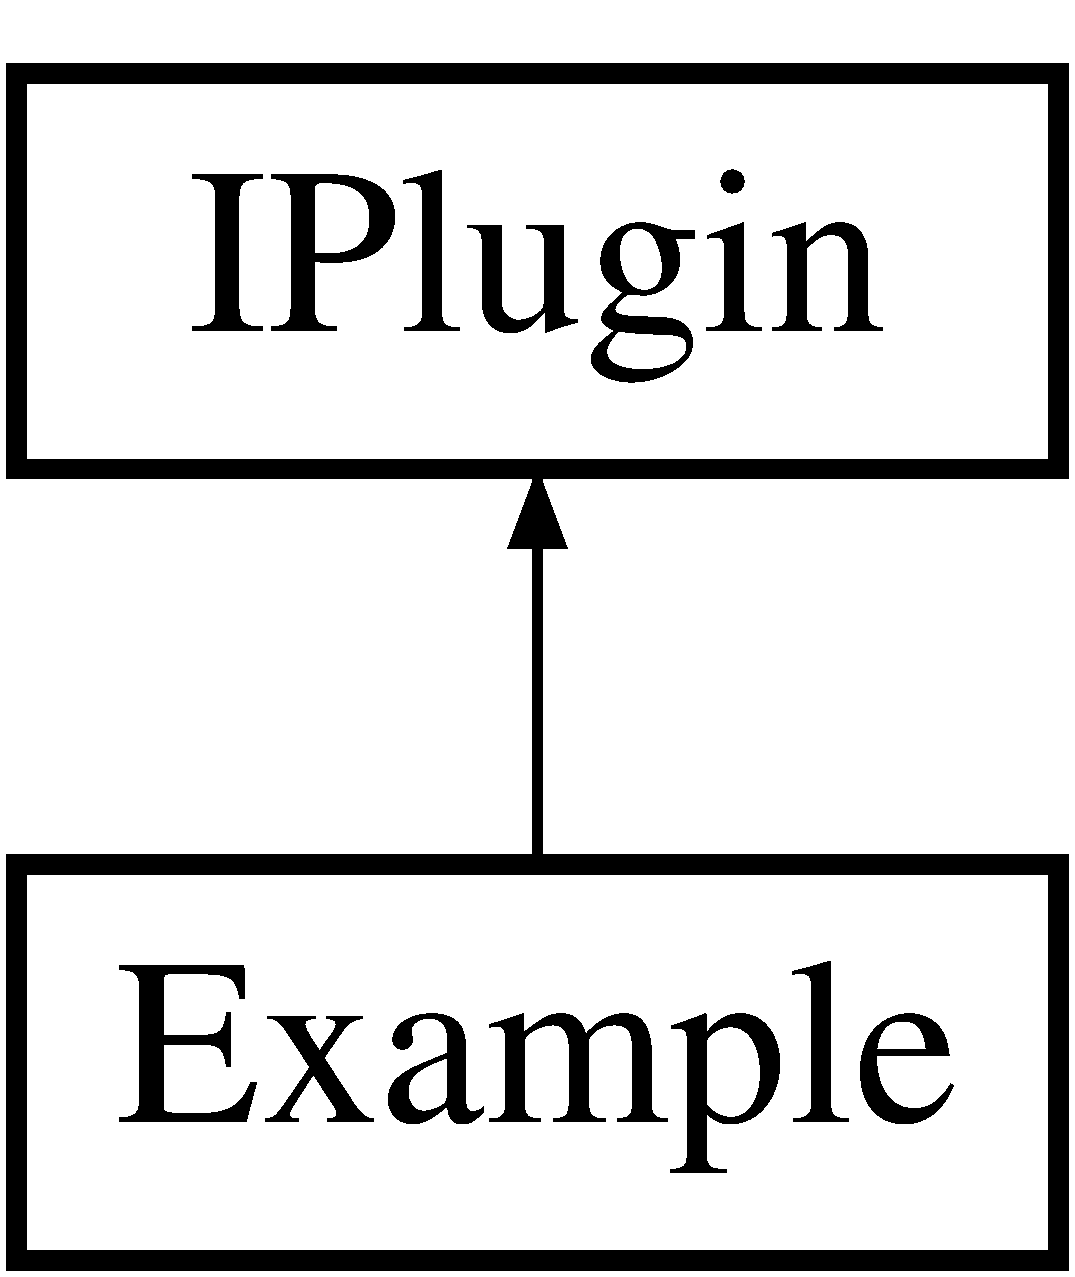
\includegraphics[height=2.000000cm]{classExample}
\end{center}
\end{figure}
\subsection*{Public Member Functions}
\begin{DoxyCompactItemize}
\item 
\hyperlink{plugins_8hh_af34747f68f9b0963dea6e8f3c659659c}{plugin} \hyperlink{classExample_aaa8ffc33c65da38507a78ff0558b9a0b}{plugin\+\_\+identifier} ()
\item 
void \hyperlink{classExample_ad360c0096bec1dcc3ee3476177922b9b}{load\+\_\+plugin} ()
\item 
void \hyperlink{classExample_a56e02424701a4ece2cdaf1d78e26e1ee}{interrupt\+\_\+material\+\_\+creation} (\hyperlink{structmaterial__identifier}{material\+\_\+identifier} \&\+\_\+new\+\_\+material)
\item 
void \hyperlink{classExample_a3869ba072c8487da1c2b6bbc329780b7}{interrupt\+\_\+section\+\_\+creation} (\hyperlink{structsection__identifier}{section\+\_\+identifier} \&\+\_\+new\+\_\+section)
\item 
void \hyperlink{classExample_a9f27f6e717db44baf27a1ed29584037a}{interrupt\+\_\+node\+\_\+creation} (\hyperlink{structnode__identifier}{node\+\_\+identifier} \&\+\_\+new\+\_\+node)
\item 
void \hyperlink{classExample_a2faa03f186d79fd113db8101e46b6b47}{interrupt\+\_\+element\+\_\+creation} (\hyperlink{structelement__identifier}{element\+\_\+identifier} \&\+\_\+new\+\_\+element)
\item 
void \hyperlink{classExample_a89228b638604306864d5544808edd94d}{interrupt\+\_\+element\+\_\+link\+\_\+creation} (\hyperlink{structelement__link__identifier}{element\+\_\+link\+\_\+identifier} \&\+\_\+new\+\_\+element\+\_\+link)
\item 
void \hyperlink{classExample_a2cdb7dc01165c9816dcbf5694fa741ff}{interrupt\+\_\+pre\+\_\+simulation} ()
\item 
void \hyperlink{classExample_aea2b516017d673a4c3e1d6c92aa06f8a}{interrupt\+\_\+start\+\_\+step} (int \+\_\+step, double)
\item 
void \hyperlink{classExample_ada33e15e3a0e4ff7cfc3c1cfad26a7bf}{interrupt\+\_\+end\+\_\+step} (int \+\_\+step, double)
\item 
void \hyperlink{classExample_a3835b961774e2cd2eeae6af3e325b4be}{interrupt\+\_\+post\+\_\+simulation} ()
\end{DoxyCompactItemize}
\subsection*{Additional Inherited Members}


\subsection{Member Function Documentation}
\index{Example@{Example}!interrupt\+\_\+element\+\_\+creation@{interrupt\+\_\+element\+\_\+creation}}
\index{interrupt\+\_\+element\+\_\+creation@{interrupt\+\_\+element\+\_\+creation}!Example@{Example}}
\subsubsection[{\texorpdfstring{interrupt\+\_\+element\+\_\+creation(element\+\_\+identifier \&\+\_\+new\+\_\+element)}{interrupt_element_creation(element_identifier &_new_element)}}]{\setlength{\rightskip}{0pt plus 5cm}void Example\+::interrupt\+\_\+element\+\_\+creation (
\begin{DoxyParamCaption}
\item[{{\bf element\+\_\+identifier} \&}]{\+\_\+new\+\_\+element}
\end{DoxyParamCaption}
)\hspace{0.3cm}{\ttfamily [virtual]}}\hypertarget{classExample_a2faa03f186d79fd113db8101e46b6b47}{}\label{classExample_a2faa03f186d79fd113db8101e46b6b47}


Reimplemented from \hyperlink{classIPlugin_ac0e36a76522f4d6e2fd33d82abb25770}{I\+Plugin}.

\index{Example@{Example}!interrupt\+\_\+element\+\_\+link\+\_\+creation@{interrupt\+\_\+element\+\_\+link\+\_\+creation}}
\index{interrupt\+\_\+element\+\_\+link\+\_\+creation@{interrupt\+\_\+element\+\_\+link\+\_\+creation}!Example@{Example}}
\subsubsection[{\texorpdfstring{interrupt\+\_\+element\+\_\+link\+\_\+creation(element\+\_\+link\+\_\+identifier \&\+\_\+new\+\_\+element\+\_\+link)}{interrupt_element_link_creation(element_link_identifier &_new_element_link)}}]{\setlength{\rightskip}{0pt plus 5cm}void Example\+::interrupt\+\_\+element\+\_\+link\+\_\+creation (
\begin{DoxyParamCaption}
\item[{{\bf element\+\_\+link\+\_\+identifier} \&}]{\+\_\+new\+\_\+element\+\_\+link}
\end{DoxyParamCaption}
)\hspace{0.3cm}{\ttfamily [virtual]}}\hypertarget{classExample_a89228b638604306864d5544808edd94d}{}\label{classExample_a89228b638604306864d5544808edd94d}


Reimplemented from \hyperlink{classIPlugin_acea743d2a1b418d671d980418787ee3c}{I\+Plugin}.

\index{Example@{Example}!interrupt\+\_\+end\+\_\+step@{interrupt\+\_\+end\+\_\+step}}
\index{interrupt\+\_\+end\+\_\+step@{interrupt\+\_\+end\+\_\+step}!Example@{Example}}
\subsubsection[{\texorpdfstring{interrupt\+\_\+end\+\_\+step(int \+\_\+step, double)}{interrupt_end_step(int _step, double)}}]{\setlength{\rightskip}{0pt plus 5cm}void Example\+::interrupt\+\_\+end\+\_\+step (
\begin{DoxyParamCaption}
\item[{int}]{\+\_\+step, }
\item[{double}]{}
\end{DoxyParamCaption}
)\hspace{0.3cm}{\ttfamily [virtual]}}\hypertarget{classExample_ada33e15e3a0e4ff7cfc3c1cfad26a7bf}{}\label{classExample_ada33e15e3a0e4ff7cfc3c1cfad26a7bf}


Reimplemented from \hyperlink{classIPlugin_ada2dcfc2d2b1a67b29fe75b30575fbe6}{I\+Plugin}.

\index{Example@{Example}!interrupt\+\_\+material\+\_\+creation@{interrupt\+\_\+material\+\_\+creation}}
\index{interrupt\+\_\+material\+\_\+creation@{interrupt\+\_\+material\+\_\+creation}!Example@{Example}}
\subsubsection[{\texorpdfstring{interrupt\+\_\+material\+\_\+creation(material\+\_\+identifier \&\+\_\+new\+\_\+material)}{interrupt_material_creation(material_identifier &_new_material)}}]{\setlength{\rightskip}{0pt plus 5cm}void Example\+::interrupt\+\_\+material\+\_\+creation (
\begin{DoxyParamCaption}
\item[{{\bf material\+\_\+identifier} \&}]{\+\_\+new\+\_\+material}
\end{DoxyParamCaption}
)\hspace{0.3cm}{\ttfamily [virtual]}}\hypertarget{classExample_a56e02424701a4ece2cdaf1d78e26e1ee}{}\label{classExample_a56e02424701a4ece2cdaf1d78e26e1ee}


Reimplemented from \hyperlink{classIPlugin_ab5917f9b11793d640a5c386f8107033a}{I\+Plugin}.

\index{Example@{Example}!interrupt\+\_\+node\+\_\+creation@{interrupt\+\_\+node\+\_\+creation}}
\index{interrupt\+\_\+node\+\_\+creation@{interrupt\+\_\+node\+\_\+creation}!Example@{Example}}
\subsubsection[{\texorpdfstring{interrupt\+\_\+node\+\_\+creation(node\+\_\+identifier \&\+\_\+new\+\_\+node)}{interrupt_node_creation(node_identifier &_new_node)}}]{\setlength{\rightskip}{0pt plus 5cm}void Example\+::interrupt\+\_\+node\+\_\+creation (
\begin{DoxyParamCaption}
\item[{{\bf node\+\_\+identifier} \&}]{\+\_\+new\+\_\+node}
\end{DoxyParamCaption}
)\hspace{0.3cm}{\ttfamily [virtual]}}\hypertarget{classExample_a9f27f6e717db44baf27a1ed29584037a}{}\label{classExample_a9f27f6e717db44baf27a1ed29584037a}


Reimplemented from \hyperlink{classIPlugin_a100d2a3202e1117c81ba40da77421b9d}{I\+Plugin}.

\index{Example@{Example}!interrupt\+\_\+post\+\_\+simulation@{interrupt\+\_\+post\+\_\+simulation}}
\index{interrupt\+\_\+post\+\_\+simulation@{interrupt\+\_\+post\+\_\+simulation}!Example@{Example}}
\subsubsection[{\texorpdfstring{interrupt\+\_\+post\+\_\+simulation()}{interrupt_post_simulation()}}]{\setlength{\rightskip}{0pt plus 5cm}void Example\+::interrupt\+\_\+post\+\_\+simulation (
\begin{DoxyParamCaption}
{}
\end{DoxyParamCaption}
)\hspace{0.3cm}{\ttfamily [virtual]}}\hypertarget{classExample_a3835b961774e2cd2eeae6af3e325b4be}{}\label{classExample_a3835b961774e2cd2eeae6af3e325b4be}


Reimplemented from \hyperlink{classIPlugin_a8de731011e31780ece2990086db410a0}{I\+Plugin}.

\index{Example@{Example}!interrupt\+\_\+pre\+\_\+simulation@{interrupt\+\_\+pre\+\_\+simulation}}
\index{interrupt\+\_\+pre\+\_\+simulation@{interrupt\+\_\+pre\+\_\+simulation}!Example@{Example}}
\subsubsection[{\texorpdfstring{interrupt\+\_\+pre\+\_\+simulation()}{interrupt_pre_simulation()}}]{\setlength{\rightskip}{0pt plus 5cm}void Example\+::interrupt\+\_\+pre\+\_\+simulation (
\begin{DoxyParamCaption}
{}
\end{DoxyParamCaption}
)\hspace{0.3cm}{\ttfamily [virtual]}}\hypertarget{classExample_a2cdb7dc01165c9816dcbf5694fa741ff}{}\label{classExample_a2cdb7dc01165c9816dcbf5694fa741ff}


Reimplemented from \hyperlink{classIPlugin_af3a42960590594e2623fc2592c925de3}{I\+Plugin}.

\index{Example@{Example}!interrupt\+\_\+section\+\_\+creation@{interrupt\+\_\+section\+\_\+creation}}
\index{interrupt\+\_\+section\+\_\+creation@{interrupt\+\_\+section\+\_\+creation}!Example@{Example}}
\subsubsection[{\texorpdfstring{interrupt\+\_\+section\+\_\+creation(section\+\_\+identifier \&\+\_\+new\+\_\+section)}{interrupt_section_creation(section_identifier &_new_section)}}]{\setlength{\rightskip}{0pt plus 5cm}void Example\+::interrupt\+\_\+section\+\_\+creation (
\begin{DoxyParamCaption}
\item[{{\bf section\+\_\+identifier} \&}]{\+\_\+new\+\_\+section}
\end{DoxyParamCaption}
)\hspace{0.3cm}{\ttfamily [virtual]}}\hypertarget{classExample_a3869ba072c8487da1c2b6bbc329780b7}{}\label{classExample_a3869ba072c8487da1c2b6bbc329780b7}


Reimplemented from \hyperlink{classIPlugin_ac247d76db1677abefface875defac756}{I\+Plugin}.

\index{Example@{Example}!interrupt\+\_\+start\+\_\+step@{interrupt\+\_\+start\+\_\+step}}
\index{interrupt\+\_\+start\+\_\+step@{interrupt\+\_\+start\+\_\+step}!Example@{Example}}
\subsubsection[{\texorpdfstring{interrupt\+\_\+start\+\_\+step(int \+\_\+step, double)}{interrupt_start_step(int _step, double)}}]{\setlength{\rightskip}{0pt plus 5cm}void Example\+::interrupt\+\_\+start\+\_\+step (
\begin{DoxyParamCaption}
\item[{int}]{\+\_\+step, }
\item[{double}]{}
\end{DoxyParamCaption}
)\hspace{0.3cm}{\ttfamily [virtual]}}\hypertarget{classExample_aea2b516017d673a4c3e1d6c92aa06f8a}{}\label{classExample_aea2b516017d673a4c3e1d6c92aa06f8a}


Reimplemented from \hyperlink{classIPlugin_ab6128940f6d722d57f26c61b56d2b213}{I\+Plugin}.

\index{Example@{Example}!load\+\_\+plugin@{load\+\_\+plugin}}
\index{load\+\_\+plugin@{load\+\_\+plugin}!Example@{Example}}
\subsubsection[{\texorpdfstring{load\+\_\+plugin()}{load_plugin()}}]{\setlength{\rightskip}{0pt plus 5cm}void Example\+::load\+\_\+plugin (
\begin{DoxyParamCaption}
{}
\end{DoxyParamCaption}
)\hspace{0.3cm}{\ttfamily [virtual]}}\hypertarget{classExample_ad360c0096bec1dcc3ee3476177922b9b}{}\label{classExample_ad360c0096bec1dcc3ee3476177922b9b}


Reimplemented from \hyperlink{classIPlugin_aec5e64955d7c36f033651ff4d93d6ebb}{I\+Plugin}.

\index{Example@{Example}!plugin\+\_\+identifier@{plugin\+\_\+identifier}}
\index{plugin\+\_\+identifier@{plugin\+\_\+identifier}!Example@{Example}}
\subsubsection[{\texorpdfstring{plugin\+\_\+identifier()}{plugin_identifier()}}]{\setlength{\rightskip}{0pt plus 5cm}{\bf plugin} Example\+::plugin\+\_\+identifier (
\begin{DoxyParamCaption}
{}
\end{DoxyParamCaption}
)\hspace{0.3cm}{\ttfamily [inline]}, {\ttfamily [virtual]}}\hypertarget{classExample_aaa8ffc33c65da38507a78ff0558b9a0b}{}\label{classExample_aaa8ffc33c65da38507a78ff0558b9a0b}


Reimplemented from \hyperlink{classIPlugin_adcfd0fb076b3d72246d1dbdccecc69d6}{I\+Plugin}.



The documentation for this class was generated from the following files\+:\begin{DoxyCompactItemize}
\item 
\hyperlink{plugin-example_8hh}{plugin-\/example.\+hh}\item 
\hyperlink{plugin-example_8cc}{plugin-\/example.\+cc}\end{DoxyCompactItemize}

\hypertarget{classIPlugin}{\section{I\-Plugin Class Reference}
\label{classIPlugin}\index{I\-Plugin@{I\-Plugin}}
}


{\ttfamily \#include $<$plugins.\-hh$>$}

Inheritance diagram for I\-Plugin\-:\begin{figure}[H]
\begin{center}
\leavevmode
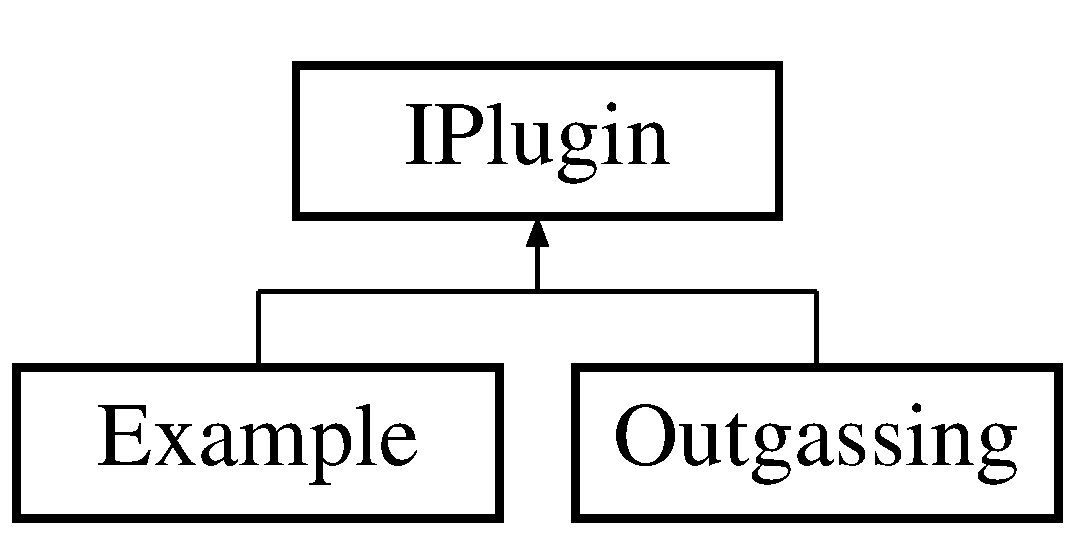
\includegraphics[height=2.000000cm]{classIPlugin}
\end{center}
\end{figure}
\subsection*{Public Member Functions}
\begin{DoxyCompactItemize}
\item 
\hyperlink{classIPlugin_a5c43c107b8a3109755cc0e5a26fb5642}{I\-Plugin} ()
\item 
virtual \hyperlink{classIPlugin_a92763c9985354dc46cae781e3873a6b2}{$\sim$\-I\-Plugin} ()
\item 
virtual \hyperlink{plugins_8hh_af34747f68f9b0963dea6e8f3c659659c}{plugin} \hyperlink{classIPlugin_adcfd0fb076b3d72246d1dbdccecc69d6}{plugin\-\_\-identifier} ()
\item 
virtual void \hyperlink{classIPlugin_aec5e64955d7c36f033651ff4d93d6ebb}{load\-\_\-plugin} ()
\item 
virtual void \hyperlink{classIPlugin_ab5917f9b11793d640a5c386f8107033a}{interrupt\-\_\-material\-\_\-creation} (\hyperlink{structmaterial__identifier}{material\-\_\-identifier} \&\-\_\-new\-\_\-material)
\item 
virtual void \hyperlink{classIPlugin_ac247d76db1677abefface875defac756}{interrupt\-\_\-section\-\_\-creation} (\hyperlink{structsection__identifier}{section\-\_\-identifier} \&\-\_\-new\-\_\-section)
\item 
virtual void \hyperlink{classIPlugin_a100d2a3202e1117c81ba40da77421b9d}{interrupt\-\_\-node\-\_\-creation} (\hyperlink{structnode__identifier}{node\-\_\-identifier} \&\-\_\-new\-\_\-node)
\item 
virtual void \hyperlink{classIPlugin_ac0e36a76522f4d6e2fd33d82abb25770}{interrupt\-\_\-element\-\_\-creation} (\hyperlink{structelement__identifier}{element\-\_\-identifier} \&\-\_\-new\-\_\-element)
\item 
virtual void \hyperlink{classIPlugin_acea743d2a1b418d671d980418787ee3c}{interrupt\-\_\-element\-\_\-link\-\_\-creation} (\hyperlink{structelement__link__identifier}{element\-\_\-link\-\_\-identifier} \&\-\_\-new\-\_\-element\-\_\-link)
\item 
virtual void \hyperlink{classIPlugin_af3a42960590594e2623fc2592c925de3}{interrupt\-\_\-pre\-\_\-simulation} ()
\item 
virtual void \hyperlink{classIPlugin_ab6128940f6d722d57f26c61b56d2b213}{interrupt\-\_\-start\-\_\-step} (int \-\_\-step, double \-\_\-time)
\item 
virtual void \hyperlink{classIPlugin_ada2dcfc2d2b1a67b29fe75b30575fbe6}{interrupt\-\_\-end\-\_\-step} (int \-\_\-step, double \-\_\-time)
\item 
virtual void \hyperlink{classIPlugin_a8de731011e31780ece2990086db410a0}{interrupt\-\_\-post\-\_\-simulation} ()
\end{DoxyCompactItemize}
\subsection*{Static Public Member Functions}
\begin{DoxyCompactItemize}
\item 
static void \hyperlink{classIPlugin_a71df92f53107b9bcd192b5350015564a}{replace\-\_\-material} (\hyperlink{structmaterial__identifier}{material\-\_\-identifier} \&\-\_\-old\-\_\-material, \hyperlink{classtds__material}{tds\-\_\-material} $\ast$\-\_\-new\-\_\-material)
\item 
static void \hyperlink{classIPlugin_a556bd8c06154fd0c8d242716800a1cbd}{replace\-\_\-section} (\hyperlink{structsection__identifier}{section\-\_\-identifier} \&\-\_\-old\-\_\-section, \hyperlink{classtds__section}{tds\-\_\-section} $\ast$\-\_\-new\-\_\-section)
\item 
static void \hyperlink{classIPlugin_af24478525e3d6e2ae4f1ea4c0a45447f}{replace\-\_\-node} (\hyperlink{structnode__identifier}{node\-\_\-identifier} \&\-\_\-old\-\_\-node, \hyperlink{classtds__node}{tds\-\_\-node} $\ast$\-\_\-new\-\_\-node)
\item 
static void \hyperlink{classIPlugin_a2d54b9b3448793b0727fadbc88c4a638}{replace\-\_\-element} (\hyperlink{structelement__identifier}{element\-\_\-identifier} \&\-\_\-old\-\_\-element, \hyperlink{classtds__element}{tds\-\_\-element} $\ast$\-\_\-new\-\_\-element)
\item 
static void \hyperlink{classIPlugin_a69d193a4010c669c8fcab69e65aa71cc}{replace\-\_\-element\-\_\-link} (\hyperlink{structelement__link__identifier}{element\-\_\-link\-\_\-identifier} \&\-\_\-old\-\_\-element\-\_\-link, \hyperlink{classtds__element__link}{tds\-\_\-element\-\_\-link} $\ast$\-\_\-new\-\_\-element\-\_\-link)
\item 
static void \hyperlink{classIPlugin_a580c91846f40f7a7f0c8d6819af66c42}{store\-\_\-plugin} (\hyperlink{classIPlugin}{I\-Plugin} $\ast$\-\_\-plugin)
\item 
static \hyperlink{classIPlugin}{I\-Plugin} $\ast$ \hyperlink{classIPlugin_a556f56970ad0bfcaf7f9fa58332a471c}{get\-\_\-plugin} (\hyperlink{plugins_8hh_af34747f68f9b0963dea6e8f3c659659c}{plugin} \-\_\-plugin\-\_\-type)
\item 
static std\-::map$<$ \hyperlink{plugins_8hh_af34747f68f9b0963dea6e8f3c659659c}{plugin}, \\*
\hyperlink{classIPlugin}{I\-Plugin} $\ast$ $>$\-::iterator \hyperlink{classIPlugin_a1d69f3981baaa8a18abd6ba5f417f6d2}{get\-\_\-plugin\-\_\-iterator} ()
\item 
static std\-::map$<$ \hyperlink{plugins_8hh_af34747f68f9b0963dea6e8f3c659659c}{plugin}, \\*
\hyperlink{classIPlugin}{I\-Plugin} $\ast$ $>$\-::iterator \hyperlink{classIPlugin_ac51f75126c8adeaaa99d48a9928deadc}{get\-\_\-plugin\-\_\-iterator\-\_\-end} ()
\item 
static bool \hyperlink{classIPlugin_a88c057bc9286f990989add575041f732}{plugin\-\_\-loaded} (\hyperlink{plugins_8hh_af34747f68f9b0963dea6e8f3c659659c}{plugin} \-\_\-plugin\-\_\-type)
\item 
static void \hyperlink{classIPlugin_a878b27eb997e500deae3df6c168b98fc}{set\-\_\-run} (\hyperlink{classtds__run}{tds\-\_\-run} $\ast$\-\_\-tds\-\_\-run)
\item 
static \hyperlink{classtds__run}{tds\-\_\-run} $\ast$ \hyperlink{classIPlugin_af887de8019efe4bb72c4ac9c5b72de71}{get\-\_\-run} ()
\end{DoxyCompactItemize}


\subsection{Constructor \& Destructor Documentation}
\hypertarget{classIPlugin_a5c43c107b8a3109755cc0e5a26fb5642}{\index{I\-Plugin@{I\-Plugin}!I\-Plugin@{I\-Plugin}}
\index{I\-Plugin@{I\-Plugin}!IPlugin@{I\-Plugin}}
\subsubsection[{I\-Plugin}]{\setlength{\rightskip}{0pt plus 5cm}I\-Plugin\-::\-I\-Plugin (
\begin{DoxyParamCaption}
{}
\end{DoxyParamCaption}
)}}\label{classIPlugin_a5c43c107b8a3109755cc0e5a26fb5642}
\hypertarget{classIPlugin_a92763c9985354dc46cae781e3873a6b2}{\index{I\-Plugin@{I\-Plugin}!$\sim$\-I\-Plugin@{$\sim$\-I\-Plugin}}
\index{$\sim$\-I\-Plugin@{$\sim$\-I\-Plugin}!IPlugin@{I\-Plugin}}
\subsubsection[{$\sim$\-I\-Plugin}]{\setlength{\rightskip}{0pt plus 5cm}I\-Plugin\-::$\sim$\-I\-Plugin (
\begin{DoxyParamCaption}
{}
\end{DoxyParamCaption}
)\hspace{0.3cm}{\ttfamily [virtual]}}}\label{classIPlugin_a92763c9985354dc46cae781e3873a6b2}


\subsection{Member Function Documentation}
\hypertarget{classIPlugin_a556f56970ad0bfcaf7f9fa58332a471c}{\index{I\-Plugin@{I\-Plugin}!get\-\_\-plugin@{get\-\_\-plugin}}
\index{get\-\_\-plugin@{get\-\_\-plugin}!IPlugin@{I\-Plugin}}
\subsubsection[{get\-\_\-plugin}]{\setlength{\rightskip}{0pt plus 5cm}{\bf I\-Plugin} $\ast$ I\-Plugin\-::get\-\_\-plugin (
\begin{DoxyParamCaption}
\item[{{\bf plugin}}]{\-\_\-plugin\-\_\-type}
\end{DoxyParamCaption}
)\hspace{0.3cm}{\ttfamily [static]}}}\label{classIPlugin_a556f56970ad0bfcaf7f9fa58332a471c}
\hypertarget{classIPlugin_a1d69f3981baaa8a18abd6ba5f417f6d2}{\index{I\-Plugin@{I\-Plugin}!get\-\_\-plugin\-\_\-iterator@{get\-\_\-plugin\-\_\-iterator}}
\index{get\-\_\-plugin\-\_\-iterator@{get\-\_\-plugin\-\_\-iterator}!IPlugin@{I\-Plugin}}
\subsubsection[{get\-\_\-plugin\-\_\-iterator}]{\setlength{\rightskip}{0pt plus 5cm}std\-::map$<$ {\bf plugin}, {\bf I\-Plugin} $\ast$ $>$\-::iterator I\-Plugin\-::get\-\_\-plugin\-\_\-iterator (
\begin{DoxyParamCaption}
{}
\end{DoxyParamCaption}
)\hspace{0.3cm}{\ttfamily [static]}}}\label{classIPlugin_a1d69f3981baaa8a18abd6ba5f417f6d2}
\hypertarget{classIPlugin_ac51f75126c8adeaaa99d48a9928deadc}{\index{I\-Plugin@{I\-Plugin}!get\-\_\-plugin\-\_\-iterator\-\_\-end@{get\-\_\-plugin\-\_\-iterator\-\_\-end}}
\index{get\-\_\-plugin\-\_\-iterator\-\_\-end@{get\-\_\-plugin\-\_\-iterator\-\_\-end}!IPlugin@{I\-Plugin}}
\subsubsection[{get\-\_\-plugin\-\_\-iterator\-\_\-end}]{\setlength{\rightskip}{0pt plus 5cm}std\-::map$<$ {\bf plugin}, {\bf I\-Plugin} $\ast$ $>$\-::iterator I\-Plugin\-::get\-\_\-plugin\-\_\-iterator\-\_\-end (
\begin{DoxyParamCaption}
{}
\end{DoxyParamCaption}
)\hspace{0.3cm}{\ttfamily [static]}}}\label{classIPlugin_ac51f75126c8adeaaa99d48a9928deadc}
\hypertarget{classIPlugin_af887de8019efe4bb72c4ac9c5b72de71}{\index{I\-Plugin@{I\-Plugin}!get\-\_\-run@{get\-\_\-run}}
\index{get\-\_\-run@{get\-\_\-run}!IPlugin@{I\-Plugin}}
\subsubsection[{get\-\_\-run}]{\setlength{\rightskip}{0pt plus 5cm}{\bf tds\-\_\-run} $\ast$ I\-Plugin\-::get\-\_\-run (
\begin{DoxyParamCaption}
{}
\end{DoxyParamCaption}
)\hspace{0.3cm}{\ttfamily [static]}}}\label{classIPlugin_af887de8019efe4bb72c4ac9c5b72de71}
\hypertarget{classIPlugin_ac0e36a76522f4d6e2fd33d82abb25770}{\index{I\-Plugin@{I\-Plugin}!interrupt\-\_\-element\-\_\-creation@{interrupt\-\_\-element\-\_\-creation}}
\index{interrupt\-\_\-element\-\_\-creation@{interrupt\-\_\-element\-\_\-creation}!IPlugin@{I\-Plugin}}
\subsubsection[{interrupt\-\_\-element\-\_\-creation}]{\setlength{\rightskip}{0pt plus 5cm}void I\-Plugin\-::interrupt\-\_\-element\-\_\-creation (
\begin{DoxyParamCaption}
\item[{{\bf element\-\_\-identifier} \&}]{\-\_\-new\-\_\-element}
\end{DoxyParamCaption}
)\hspace{0.3cm}{\ttfamily [virtual]}}}\label{classIPlugin_ac0e36a76522f4d6e2fd33d82abb25770}


Reimplemented in \hyperlink{classExample_a2faa03f186d79fd113db8101e46b6b47}{Example}.

\hypertarget{classIPlugin_acea743d2a1b418d671d980418787ee3c}{\index{I\-Plugin@{I\-Plugin}!interrupt\-\_\-element\-\_\-link\-\_\-creation@{interrupt\-\_\-element\-\_\-link\-\_\-creation}}
\index{interrupt\-\_\-element\-\_\-link\-\_\-creation@{interrupt\-\_\-element\-\_\-link\-\_\-creation}!IPlugin@{I\-Plugin}}
\subsubsection[{interrupt\-\_\-element\-\_\-link\-\_\-creation}]{\setlength{\rightskip}{0pt plus 5cm}void I\-Plugin\-::interrupt\-\_\-element\-\_\-link\-\_\-creation (
\begin{DoxyParamCaption}
\item[{{\bf element\-\_\-link\-\_\-identifier} \&}]{\-\_\-new\-\_\-element\-\_\-link}
\end{DoxyParamCaption}
)\hspace{0.3cm}{\ttfamily [virtual]}}}\label{classIPlugin_acea743d2a1b418d671d980418787ee3c}


Reimplemented in \hyperlink{classOutgassing_a71237bfa8220b867ba35a360fd5f869f}{Outgassing}, and \hyperlink{classExample_a89228b638604306864d5544808edd94d}{Example}.

\hypertarget{classIPlugin_ada2dcfc2d2b1a67b29fe75b30575fbe6}{\index{I\-Plugin@{I\-Plugin}!interrupt\-\_\-end\-\_\-step@{interrupt\-\_\-end\-\_\-step}}
\index{interrupt\-\_\-end\-\_\-step@{interrupt\-\_\-end\-\_\-step}!IPlugin@{I\-Plugin}}
\subsubsection[{interrupt\-\_\-end\-\_\-step}]{\setlength{\rightskip}{0pt plus 5cm}void I\-Plugin\-::interrupt\-\_\-end\-\_\-step (
\begin{DoxyParamCaption}
\item[{int}]{\-\_\-step, }
\item[{double}]{\-\_\-time}
\end{DoxyParamCaption}
)\hspace{0.3cm}{\ttfamily [virtual]}}}\label{classIPlugin_ada2dcfc2d2b1a67b29fe75b30575fbe6}


Reimplemented in \hyperlink{classExample_ada33e15e3a0e4ff7cfc3c1cfad26a7bf}{Example}.

\hypertarget{classIPlugin_ab5917f9b11793d640a5c386f8107033a}{\index{I\-Plugin@{I\-Plugin}!interrupt\-\_\-material\-\_\-creation@{interrupt\-\_\-material\-\_\-creation}}
\index{interrupt\-\_\-material\-\_\-creation@{interrupt\-\_\-material\-\_\-creation}!IPlugin@{I\-Plugin}}
\subsubsection[{interrupt\-\_\-material\-\_\-creation}]{\setlength{\rightskip}{0pt plus 5cm}void I\-Plugin\-::interrupt\-\_\-material\-\_\-creation (
\begin{DoxyParamCaption}
\item[{{\bf material\-\_\-identifier} \&}]{\-\_\-new\-\_\-material}
\end{DoxyParamCaption}
)\hspace{0.3cm}{\ttfamily [virtual]}}}\label{classIPlugin_ab5917f9b11793d640a5c386f8107033a}


Reimplemented in \hyperlink{classExample_a56e02424701a4ece2cdaf1d78e26e1ee}{Example}.

\hypertarget{classIPlugin_a100d2a3202e1117c81ba40da77421b9d}{\index{I\-Plugin@{I\-Plugin}!interrupt\-\_\-node\-\_\-creation@{interrupt\-\_\-node\-\_\-creation}}
\index{interrupt\-\_\-node\-\_\-creation@{interrupt\-\_\-node\-\_\-creation}!IPlugin@{I\-Plugin}}
\subsubsection[{interrupt\-\_\-node\-\_\-creation}]{\setlength{\rightskip}{0pt plus 5cm}void I\-Plugin\-::interrupt\-\_\-node\-\_\-creation (
\begin{DoxyParamCaption}
\item[{{\bf node\-\_\-identifier} \&}]{\-\_\-new\-\_\-node}
\end{DoxyParamCaption}
)\hspace{0.3cm}{\ttfamily [virtual]}}}\label{classIPlugin_a100d2a3202e1117c81ba40da77421b9d}


Reimplemented in \hyperlink{classExample_a9f27f6e717db44baf27a1ed29584037a}{Example}.

\hypertarget{classIPlugin_a8de731011e31780ece2990086db410a0}{\index{I\-Plugin@{I\-Plugin}!interrupt\-\_\-post\-\_\-simulation@{interrupt\-\_\-post\-\_\-simulation}}
\index{interrupt\-\_\-post\-\_\-simulation@{interrupt\-\_\-post\-\_\-simulation}!IPlugin@{I\-Plugin}}
\subsubsection[{interrupt\-\_\-post\-\_\-simulation}]{\setlength{\rightskip}{0pt plus 5cm}void I\-Plugin\-::interrupt\-\_\-post\-\_\-simulation (
\begin{DoxyParamCaption}
{}
\end{DoxyParamCaption}
)\hspace{0.3cm}{\ttfamily [virtual]}}}\label{classIPlugin_a8de731011e31780ece2990086db410a0}


Reimplemented in \hyperlink{classExample_a3835b961774e2cd2eeae6af3e325b4be}{Example}, and \hyperlink{classOutgassing_a1c3cb8741c2cdc09e807db1d77a3808a}{Outgassing}.

\hypertarget{classIPlugin_af3a42960590594e2623fc2592c925de3}{\index{I\-Plugin@{I\-Plugin}!interrupt\-\_\-pre\-\_\-simulation@{interrupt\-\_\-pre\-\_\-simulation}}
\index{interrupt\-\_\-pre\-\_\-simulation@{interrupt\-\_\-pre\-\_\-simulation}!IPlugin@{I\-Plugin}}
\subsubsection[{interrupt\-\_\-pre\-\_\-simulation}]{\setlength{\rightskip}{0pt plus 5cm}void I\-Plugin\-::interrupt\-\_\-pre\-\_\-simulation (
\begin{DoxyParamCaption}
{}
\end{DoxyParamCaption}
)\hspace{0.3cm}{\ttfamily [virtual]}}}\label{classIPlugin_af3a42960590594e2623fc2592c925de3}


Reimplemented in \hyperlink{classOutgassing_a7c51e9f9622f1533904efc719b353f55}{Outgassing}, and \hyperlink{classExample_a2cdb7dc01165c9816dcbf5694fa741ff}{Example}.

\hypertarget{classIPlugin_ac247d76db1677abefface875defac756}{\index{I\-Plugin@{I\-Plugin}!interrupt\-\_\-section\-\_\-creation@{interrupt\-\_\-section\-\_\-creation}}
\index{interrupt\-\_\-section\-\_\-creation@{interrupt\-\_\-section\-\_\-creation}!IPlugin@{I\-Plugin}}
\subsubsection[{interrupt\-\_\-section\-\_\-creation}]{\setlength{\rightskip}{0pt plus 5cm}void I\-Plugin\-::interrupt\-\_\-section\-\_\-creation (
\begin{DoxyParamCaption}
\item[{{\bf section\-\_\-identifier} \&}]{\-\_\-new\-\_\-section}
\end{DoxyParamCaption}
)\hspace{0.3cm}{\ttfamily [virtual]}}}\label{classIPlugin_ac247d76db1677abefface875defac756}


Reimplemented in \hyperlink{classOutgassing_a5a1afcb787654cb41df8ee91f88dee21}{Outgassing}, and \hyperlink{classExample_a3869ba072c8487da1c2b6bbc329780b7}{Example}.

\hypertarget{classIPlugin_ab6128940f6d722d57f26c61b56d2b213}{\index{I\-Plugin@{I\-Plugin}!interrupt\-\_\-start\-\_\-step@{interrupt\-\_\-start\-\_\-step}}
\index{interrupt\-\_\-start\-\_\-step@{interrupt\-\_\-start\-\_\-step}!IPlugin@{I\-Plugin}}
\subsubsection[{interrupt\-\_\-start\-\_\-step}]{\setlength{\rightskip}{0pt plus 5cm}void I\-Plugin\-::interrupt\-\_\-start\-\_\-step (
\begin{DoxyParamCaption}
\item[{int}]{\-\_\-step, }
\item[{double}]{\-\_\-time}
\end{DoxyParamCaption}
)\hspace{0.3cm}{\ttfamily [virtual]}}}\label{classIPlugin_ab6128940f6d722d57f26c61b56d2b213}


Reimplemented in \hyperlink{classExample_aea2b516017d673a4c3e1d6c92aa06f8a}{Example}.

\hypertarget{classIPlugin_aec5e64955d7c36f033651ff4d93d6ebb}{\index{I\-Plugin@{I\-Plugin}!load\-\_\-plugin@{load\-\_\-plugin}}
\index{load\-\_\-plugin@{load\-\_\-plugin}!IPlugin@{I\-Plugin}}
\subsubsection[{load\-\_\-plugin}]{\setlength{\rightskip}{0pt plus 5cm}void I\-Plugin\-::load\-\_\-plugin (
\begin{DoxyParamCaption}
{}
\end{DoxyParamCaption}
)\hspace{0.3cm}{\ttfamily [virtual]}}}\label{classIPlugin_aec5e64955d7c36f033651ff4d93d6ebb}


Reimplemented in \hyperlink{classOutgassing_aa999ed92df7cc8858da8f877db1c6bf3}{Outgassing}, and \hyperlink{classExample_ad360c0096bec1dcc3ee3476177922b9b}{Example}.

\hypertarget{classIPlugin_adcfd0fb076b3d72246d1dbdccecc69d6}{\index{I\-Plugin@{I\-Plugin}!plugin\-\_\-identifier@{plugin\-\_\-identifier}}
\index{plugin\-\_\-identifier@{plugin\-\_\-identifier}!IPlugin@{I\-Plugin}}
\subsubsection[{plugin\-\_\-identifier}]{\setlength{\rightskip}{0pt plus 5cm}{\bf plugin} I\-Plugin\-::plugin\-\_\-identifier (
\begin{DoxyParamCaption}
{}
\end{DoxyParamCaption}
)\hspace{0.3cm}{\ttfamily [virtual]}}}\label{classIPlugin_adcfd0fb076b3d72246d1dbdccecc69d6}


Reimplemented in \hyperlink{classOutgassing_a35c522220af5add597f30bcf2a07df68}{Outgassing}, and \hyperlink{classExample_aaa8ffc33c65da38507a78ff0558b9a0b}{Example}.

\hypertarget{classIPlugin_a88c057bc9286f990989add575041f732}{\index{I\-Plugin@{I\-Plugin}!plugin\-\_\-loaded@{plugin\-\_\-loaded}}
\index{plugin\-\_\-loaded@{plugin\-\_\-loaded}!IPlugin@{I\-Plugin}}
\subsubsection[{plugin\-\_\-loaded}]{\setlength{\rightskip}{0pt plus 5cm}bool I\-Plugin\-::plugin\-\_\-loaded (
\begin{DoxyParamCaption}
\item[{{\bf plugin}}]{\-\_\-plugin\-\_\-type}
\end{DoxyParamCaption}
)\hspace{0.3cm}{\ttfamily [static]}}}\label{classIPlugin_a88c057bc9286f990989add575041f732}
\hypertarget{classIPlugin_a2d54b9b3448793b0727fadbc88c4a638}{\index{I\-Plugin@{I\-Plugin}!replace\-\_\-element@{replace\-\_\-element}}
\index{replace\-\_\-element@{replace\-\_\-element}!IPlugin@{I\-Plugin}}
\subsubsection[{replace\-\_\-element}]{\setlength{\rightskip}{0pt plus 5cm}void I\-Plugin\-::replace\-\_\-element (
\begin{DoxyParamCaption}
\item[{{\bf element\-\_\-identifier} \&}]{\-\_\-old\-\_\-element, }
\item[{{\bf tds\-\_\-element} $\ast$}]{\-\_\-new\-\_\-element}
\end{DoxyParamCaption}
)\hspace{0.3cm}{\ttfamily [static]}}}\label{classIPlugin_a2d54b9b3448793b0727fadbc88c4a638}
\hypertarget{classIPlugin_a69d193a4010c669c8fcab69e65aa71cc}{\index{I\-Plugin@{I\-Plugin}!replace\-\_\-element\-\_\-link@{replace\-\_\-element\-\_\-link}}
\index{replace\-\_\-element\-\_\-link@{replace\-\_\-element\-\_\-link}!IPlugin@{I\-Plugin}}
\subsubsection[{replace\-\_\-element\-\_\-link}]{\setlength{\rightskip}{0pt plus 5cm}void I\-Plugin\-::replace\-\_\-element\-\_\-link (
\begin{DoxyParamCaption}
\item[{{\bf element\-\_\-link\-\_\-identifier} \&}]{\-\_\-old\-\_\-element\-\_\-link, }
\item[{{\bf tds\-\_\-element\-\_\-link} $\ast$}]{\-\_\-new\-\_\-element\-\_\-link}
\end{DoxyParamCaption}
)\hspace{0.3cm}{\ttfamily [static]}}}\label{classIPlugin_a69d193a4010c669c8fcab69e65aa71cc}
\hypertarget{classIPlugin_a71df92f53107b9bcd192b5350015564a}{\index{I\-Plugin@{I\-Plugin}!replace\-\_\-material@{replace\-\_\-material}}
\index{replace\-\_\-material@{replace\-\_\-material}!IPlugin@{I\-Plugin}}
\subsubsection[{replace\-\_\-material}]{\setlength{\rightskip}{0pt plus 5cm}void I\-Plugin\-::replace\-\_\-material (
\begin{DoxyParamCaption}
\item[{{\bf material\-\_\-identifier} \&}]{\-\_\-old\-\_\-material, }
\item[{{\bf tds\-\_\-material} $\ast$}]{\-\_\-new\-\_\-material}
\end{DoxyParamCaption}
)\hspace{0.3cm}{\ttfamily [static]}}}\label{classIPlugin_a71df92f53107b9bcd192b5350015564a}
\hypertarget{classIPlugin_af24478525e3d6e2ae4f1ea4c0a45447f}{\index{I\-Plugin@{I\-Plugin}!replace\-\_\-node@{replace\-\_\-node}}
\index{replace\-\_\-node@{replace\-\_\-node}!IPlugin@{I\-Plugin}}
\subsubsection[{replace\-\_\-node}]{\setlength{\rightskip}{0pt plus 5cm}void I\-Plugin\-::replace\-\_\-node (
\begin{DoxyParamCaption}
\item[{{\bf node\-\_\-identifier} \&}]{\-\_\-old\-\_\-node, }
\item[{{\bf tds\-\_\-node} $\ast$}]{\-\_\-new\-\_\-node}
\end{DoxyParamCaption}
)\hspace{0.3cm}{\ttfamily [static]}}}\label{classIPlugin_af24478525e3d6e2ae4f1ea4c0a45447f}
\hypertarget{classIPlugin_a556bd8c06154fd0c8d242716800a1cbd}{\index{I\-Plugin@{I\-Plugin}!replace\-\_\-section@{replace\-\_\-section}}
\index{replace\-\_\-section@{replace\-\_\-section}!IPlugin@{I\-Plugin}}
\subsubsection[{replace\-\_\-section}]{\setlength{\rightskip}{0pt plus 5cm}void I\-Plugin\-::replace\-\_\-section (
\begin{DoxyParamCaption}
\item[{{\bf section\-\_\-identifier} \&}]{\-\_\-old\-\_\-section, }
\item[{{\bf tds\-\_\-section} $\ast$}]{\-\_\-new\-\_\-section}
\end{DoxyParamCaption}
)\hspace{0.3cm}{\ttfamily [static]}}}\label{classIPlugin_a556bd8c06154fd0c8d242716800a1cbd}
\hypertarget{classIPlugin_a878b27eb997e500deae3df6c168b98fc}{\index{I\-Plugin@{I\-Plugin}!set\-\_\-run@{set\-\_\-run}}
\index{set\-\_\-run@{set\-\_\-run}!IPlugin@{I\-Plugin}}
\subsubsection[{set\-\_\-run}]{\setlength{\rightskip}{0pt plus 5cm}void I\-Plugin\-::set\-\_\-run (
\begin{DoxyParamCaption}
\item[{{\bf tds\-\_\-run} $\ast$}]{\-\_\-tds\-\_\-run}
\end{DoxyParamCaption}
)\hspace{0.3cm}{\ttfamily [static]}}}\label{classIPlugin_a878b27eb997e500deae3df6c168b98fc}
\hypertarget{classIPlugin_a580c91846f40f7a7f0c8d6819af66c42}{\index{I\-Plugin@{I\-Plugin}!store\-\_\-plugin@{store\-\_\-plugin}}
\index{store\-\_\-plugin@{store\-\_\-plugin}!IPlugin@{I\-Plugin}}
\subsubsection[{store\-\_\-plugin}]{\setlength{\rightskip}{0pt plus 5cm}void I\-Plugin\-::store\-\_\-plugin (
\begin{DoxyParamCaption}
\item[{{\bf I\-Plugin} $\ast$}]{\-\_\-plugin}
\end{DoxyParamCaption}
)\hspace{0.3cm}{\ttfamily [static]}}}\label{classIPlugin_a580c91846f40f7a7f0c8d6819af66c42}


The documentation for this class was generated from the following files\-:\begin{DoxyCompactItemize}
\item 
\hyperlink{plugins_8hh}{plugins.\-hh}\item 
\hyperlink{plugins_8cc}{plugins.\-cc}\end{DoxyCompactItemize}

\hypertarget{structmaterial__identifier}{\section{material\-\_\-identifier Struct Reference}
\label{structmaterial__identifier}\index{material\-\_\-identifier@{material\-\_\-identifier}}
}


{\ttfamily \#include $<$identifiers.\-hh$>$}

\subsection*{Public Attributes}
\begin{DoxyCompactItemize}
\item 
int \hyperlink{structmaterial__identifier_a0a78177622843fe4acef33c396737e03}{material\-\_\-id}
\item 
\hyperlink{classtds__material}{tds\-\_\-material} $\ast$ \hyperlink{structmaterial__identifier_a7721b745f0f7d8f365d0b38144e115eb}{material}
\end{DoxyCompactItemize}


\subsection{Member Data Documentation}
\hypertarget{structmaterial__identifier_a7721b745f0f7d8f365d0b38144e115eb}{\index{material\-\_\-identifier@{material\-\_\-identifier}!material@{material}}
\index{material@{material}!material_identifier@{material\-\_\-identifier}}
\subsubsection[{material}]{\setlength{\rightskip}{0pt plus 5cm}{\bf tds\-\_\-material}$\ast$ material\-\_\-identifier\-::material}}\label{structmaterial__identifier_a7721b745f0f7d8f365d0b38144e115eb}
\hypertarget{structmaterial__identifier_a0a78177622843fe4acef33c396737e03}{\index{material\-\_\-identifier@{material\-\_\-identifier}!material\-\_\-id@{material\-\_\-id}}
\index{material\-\_\-id@{material\-\_\-id}!material_identifier@{material\-\_\-identifier}}
\subsubsection[{material\-\_\-id}]{\setlength{\rightskip}{0pt plus 5cm}int material\-\_\-identifier\-::material\-\_\-id}}\label{structmaterial__identifier_a0a78177622843fe4acef33c396737e03}


The documentation for this struct was generated from the following file\-:\begin{DoxyCompactItemize}
\item 
\hyperlink{identifiers_8hh}{identifiers.\-hh}\end{DoxyCompactItemize}

\hypertarget{structnode__identifier}{\section{node\-\_\-identifier Struct Reference}
\label{structnode__identifier}\index{node\-\_\-identifier@{node\-\_\-identifier}}
}


{\ttfamily \#include $<$identifiers.\-hh$>$}

\subsection*{Public Attributes}
\begin{DoxyCompactItemize}
\item 
int \hyperlink{structnode__identifier_aeb6689eabdda3bc30e7c385940fbdf23}{node\-\_\-id}
\item 
\hyperlink{classtds__node}{tds\-\_\-node} $\ast$ \hyperlink{structnode__identifier_ac7c3a08e75cfd2cec2decd099c1577b3}{node}
\end{DoxyCompactItemize}


\subsection{Member Data Documentation}
\hypertarget{structnode__identifier_ac7c3a08e75cfd2cec2decd099c1577b3}{\index{node\-\_\-identifier@{node\-\_\-identifier}!node@{node}}
\index{node@{node}!node_identifier@{node\-\_\-identifier}}
\subsubsection[{node}]{\setlength{\rightskip}{0pt plus 5cm}{\bf tds\-\_\-node}$\ast$ node\-\_\-identifier\-::node}}\label{structnode__identifier_ac7c3a08e75cfd2cec2decd099c1577b3}
\hypertarget{structnode__identifier_aeb6689eabdda3bc30e7c385940fbdf23}{\index{node\-\_\-identifier@{node\-\_\-identifier}!node\-\_\-id@{node\-\_\-id}}
\index{node\-\_\-id@{node\-\_\-id}!node_identifier@{node\-\_\-identifier}}
\subsubsection[{node\-\_\-id}]{\setlength{\rightskip}{0pt plus 5cm}int node\-\_\-identifier\-::node\-\_\-id}}\label{structnode__identifier_aeb6689eabdda3bc30e7c385940fbdf23}


The documentation for this struct was generated from the following file\-:\begin{DoxyCompactItemize}
\item 
\hyperlink{identifiers_8hh}{identifiers.\-hh}\end{DoxyCompactItemize}

\hypertarget{classOutgassing}{\section{Outgassing Class Reference}
\label{classOutgassing}\index{Outgassing@{Outgassing}}
}


{\ttfamily \#include $<$plugin-\/outgassing.\-hh$>$}

Inheritance diagram for Outgassing\-:\begin{figure}[H]
\begin{center}
\leavevmode
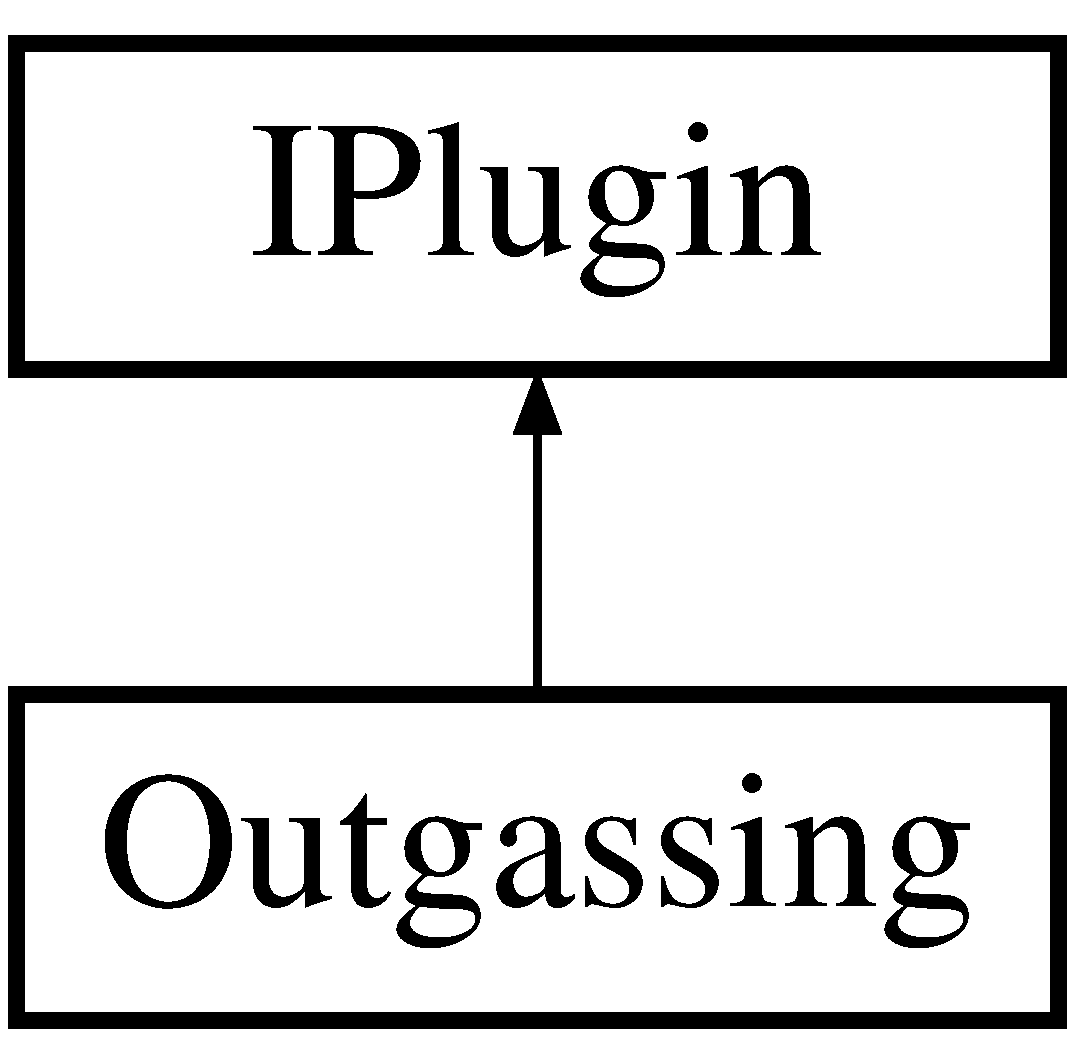
\includegraphics[height=2.000000cm]{classOutgassing}
\end{center}
\end{figure}
\subsection*{Public Member Functions}
\begin{DoxyCompactItemize}
\item 
\hyperlink{plugins_8hh_af34747f68f9b0963dea6e8f3c659659c}{plugin} \hyperlink{classOutgassing_a35c522220af5add597f30bcf2a07df68}{plugin\-\_\-identifier} ()
\item 
void \hyperlink{classOutgassing_aa999ed92df7cc8858da8f877db1c6bf3}{load\-\_\-plugin} ()
\item 
void \hyperlink{classOutgassing_a5a1afcb787654cb41df8ee91f88dee21}{interrupt\-\_\-section\-\_\-creation} (\hyperlink{structsection__identifier}{section\-\_\-identifier} \&\-\_\-new\-\_\-section)
\item 
void \hyperlink{classOutgassing_a71237bfa8220b867ba35a360fd5f869f}{interrupt\-\_\-element\-\_\-link\-\_\-creation} (\hyperlink{structelement__link__identifier}{element\-\_\-link\-\_\-identifier} \&\-\_\-new\-\_\-element\-\_\-link)
\item 
void \hyperlink{classOutgassing_a7c51e9f9622f1533904efc719b353f55}{interrupt\-\_\-pre\-\_\-simulation} ()
\item 
void \hyperlink{classOutgassing_a1c3cb8741c2cdc09e807db1d77a3808a}{interrupt\-\_\-post\-\_\-simulation} ()
\end{DoxyCompactItemize}
\subsection*{Additional Inherited Members}


\subsection{Member Function Documentation}
\hypertarget{classOutgassing_a71237bfa8220b867ba35a360fd5f869f}{\index{Outgassing@{Outgassing}!interrupt\-\_\-element\-\_\-link\-\_\-creation@{interrupt\-\_\-element\-\_\-link\-\_\-creation}}
\index{interrupt\-\_\-element\-\_\-link\-\_\-creation@{interrupt\-\_\-element\-\_\-link\-\_\-creation}!Outgassing@{Outgassing}}
\subsubsection[{interrupt\-\_\-element\-\_\-link\-\_\-creation}]{\setlength{\rightskip}{0pt plus 5cm}void Outgassing\-::interrupt\-\_\-element\-\_\-link\-\_\-creation (
\begin{DoxyParamCaption}
\item[{{\bf element\-\_\-link\-\_\-identifier} \&}]{\-\_\-new\-\_\-element\-\_\-link}
\end{DoxyParamCaption}
)\hspace{0.3cm}{\ttfamily [virtual]}}}\label{classOutgassing_a71237bfa8220b867ba35a360fd5f869f}


Reimplemented from \hyperlink{classIPlugin_acea743d2a1b418d671d980418787ee3c}{I\-Plugin}.

\hypertarget{classOutgassing_a1c3cb8741c2cdc09e807db1d77a3808a}{\index{Outgassing@{Outgassing}!interrupt\-\_\-post\-\_\-simulation@{interrupt\-\_\-post\-\_\-simulation}}
\index{interrupt\-\_\-post\-\_\-simulation@{interrupt\-\_\-post\-\_\-simulation}!Outgassing@{Outgassing}}
\subsubsection[{interrupt\-\_\-post\-\_\-simulation}]{\setlength{\rightskip}{0pt plus 5cm}void Outgassing\-::interrupt\-\_\-post\-\_\-simulation (
\begin{DoxyParamCaption}
{}
\end{DoxyParamCaption}
)\hspace{0.3cm}{\ttfamily [virtual]}}}\label{classOutgassing_a1c3cb8741c2cdc09e807db1d77a3808a}


Reimplemented from \hyperlink{classIPlugin_a8de731011e31780ece2990086db410a0}{I\-Plugin}.

\hypertarget{classOutgassing_a7c51e9f9622f1533904efc719b353f55}{\index{Outgassing@{Outgassing}!interrupt\-\_\-pre\-\_\-simulation@{interrupt\-\_\-pre\-\_\-simulation}}
\index{interrupt\-\_\-pre\-\_\-simulation@{interrupt\-\_\-pre\-\_\-simulation}!Outgassing@{Outgassing}}
\subsubsection[{interrupt\-\_\-pre\-\_\-simulation}]{\setlength{\rightskip}{0pt plus 5cm}void Outgassing\-::interrupt\-\_\-pre\-\_\-simulation (
\begin{DoxyParamCaption}
{}
\end{DoxyParamCaption}
)\hspace{0.3cm}{\ttfamily [virtual]}}}\label{classOutgassing_a7c51e9f9622f1533904efc719b353f55}


Reimplemented from \hyperlink{classIPlugin_af3a42960590594e2623fc2592c925de3}{I\-Plugin}.

\hypertarget{classOutgassing_a5a1afcb787654cb41df8ee91f88dee21}{\index{Outgassing@{Outgassing}!interrupt\-\_\-section\-\_\-creation@{interrupt\-\_\-section\-\_\-creation}}
\index{interrupt\-\_\-section\-\_\-creation@{interrupt\-\_\-section\-\_\-creation}!Outgassing@{Outgassing}}
\subsubsection[{interrupt\-\_\-section\-\_\-creation}]{\setlength{\rightskip}{0pt plus 5cm}void Outgassing\-::interrupt\-\_\-section\-\_\-creation (
\begin{DoxyParamCaption}
\item[{{\bf section\-\_\-identifier} \&}]{\-\_\-new\-\_\-section}
\end{DoxyParamCaption}
)\hspace{0.3cm}{\ttfamily [virtual]}}}\label{classOutgassing_a5a1afcb787654cb41df8ee91f88dee21}


Reimplemented from \hyperlink{classIPlugin_ac247d76db1677abefface875defac756}{I\-Plugin}.

\hypertarget{classOutgassing_aa999ed92df7cc8858da8f877db1c6bf3}{\index{Outgassing@{Outgassing}!load\-\_\-plugin@{load\-\_\-plugin}}
\index{load\-\_\-plugin@{load\-\_\-plugin}!Outgassing@{Outgassing}}
\subsubsection[{load\-\_\-plugin}]{\setlength{\rightskip}{0pt plus 5cm}void Outgassing\-::load\-\_\-plugin (
\begin{DoxyParamCaption}
{}
\end{DoxyParamCaption}
)\hspace{0.3cm}{\ttfamily [virtual]}}}\label{classOutgassing_aa999ed92df7cc8858da8f877db1c6bf3}


Reimplemented from \hyperlink{classIPlugin_aec5e64955d7c36f033651ff4d93d6ebb}{I\-Plugin}.

\hypertarget{classOutgassing_a35c522220af5add597f30bcf2a07df68}{\index{Outgassing@{Outgassing}!plugin\-\_\-identifier@{plugin\-\_\-identifier}}
\index{plugin\-\_\-identifier@{plugin\-\_\-identifier}!Outgassing@{Outgassing}}
\subsubsection[{plugin\-\_\-identifier}]{\setlength{\rightskip}{0pt plus 5cm}{\bf plugin} Outgassing\-::plugin\-\_\-identifier (
\begin{DoxyParamCaption}
{}
\end{DoxyParamCaption}
)\hspace{0.3cm}{\ttfamily [inline]}, {\ttfamily [virtual]}}}\label{classOutgassing_a35c522220af5add597f30bcf2a07df68}


Reimplemented from \hyperlink{classIPlugin_adcfd0fb076b3d72246d1dbdccecc69d6}{I\-Plugin}.



The documentation for this class was generated from the following files\-:\begin{DoxyCompactItemize}
\item 
\hyperlink{plugin-outgassing_8hh}{plugin-\/outgassing.\-hh}\item 
\hyperlink{plugin-outgassing_8cc}{plugin-\/outgassing.\-cc}\end{DoxyCompactItemize}

\hypertarget{structsection__identifier}{\section{section\-\_\-identifier Struct Reference}
\label{structsection__identifier}\index{section\-\_\-identifier@{section\-\_\-identifier}}
}


{\ttfamily \#include $<$identifiers.\-hh$>$}

\subsection*{Public Attributes}
\begin{DoxyCompactItemize}
\item 
int \hyperlink{structsection__identifier_a09ca225eec6a949e98efb59687e6b4ca}{section\-\_\-id}
\item 
\hyperlink{classtds__section}{tds\-\_\-section} $\ast$ \hyperlink{structsection__identifier_a379de132baa2a9a5949decef3e4bb85e}{section}
\end{DoxyCompactItemize}


\subsection{Member Data Documentation}
\hypertarget{structsection__identifier_a379de132baa2a9a5949decef3e4bb85e}{\index{section\-\_\-identifier@{section\-\_\-identifier}!section@{section}}
\index{section@{section}!section_identifier@{section\-\_\-identifier}}
\subsubsection[{section}]{\setlength{\rightskip}{0pt plus 5cm}{\bf tds\-\_\-section}$\ast$ section\-\_\-identifier\-::section}}\label{structsection__identifier_a379de132baa2a9a5949decef3e4bb85e}
\hypertarget{structsection__identifier_a09ca225eec6a949e98efb59687e6b4ca}{\index{section\-\_\-identifier@{section\-\_\-identifier}!section\-\_\-id@{section\-\_\-id}}
\index{section\-\_\-id@{section\-\_\-id}!section_identifier@{section\-\_\-identifier}}
\subsubsection[{section\-\_\-id}]{\setlength{\rightskip}{0pt plus 5cm}int section\-\_\-identifier\-::section\-\_\-id}}\label{structsection__identifier_a09ca225eec6a949e98efb59687e6b4ca}


The documentation for this struct was generated from the following file\-:\begin{DoxyCompactItemize}
\item 
\hyperlink{identifiers_8hh}{identifiers.\-hh}\end{DoxyCompactItemize}

\hypertarget{classtds}{\section{tds Class Reference}
\label{classtds}\index{tds@{tds}}
}


{\ttfamily \#include $<$tds.\-hh$>$}

Inheritance diagram for tds\-:\begin{figure}[H]
\begin{center}
\leavevmode
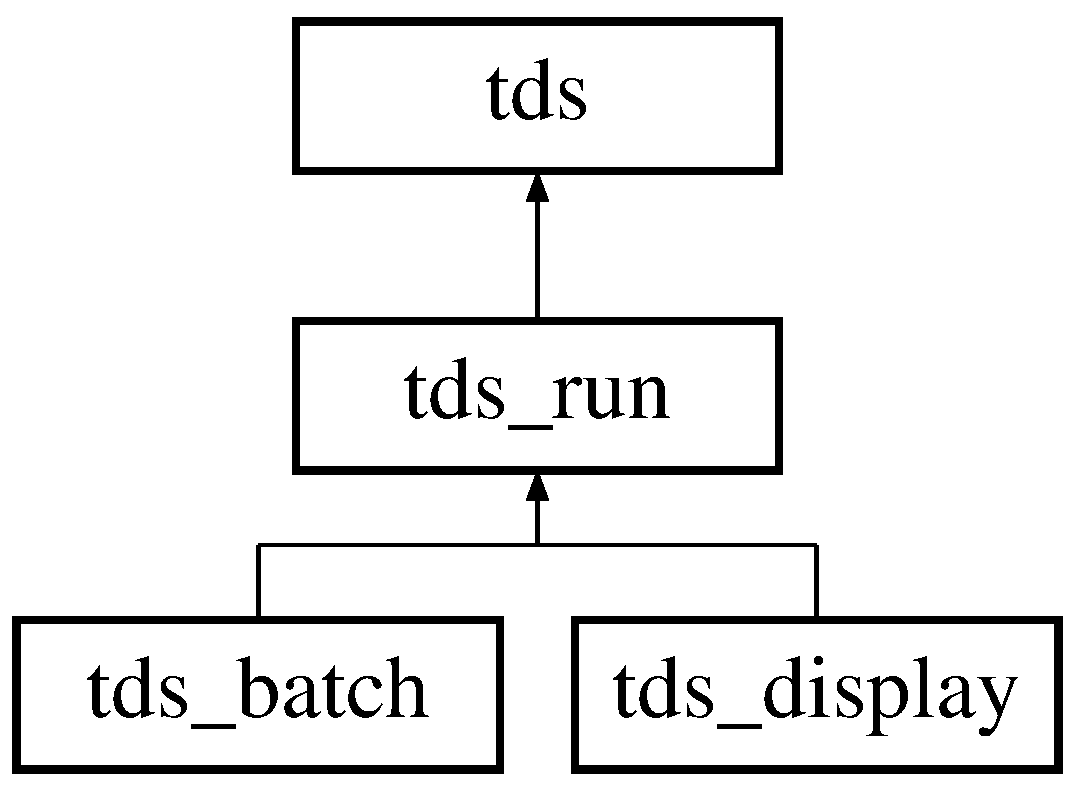
\includegraphics[height=3.000000cm]{classtds}
\end{center}
\end{figure}
\subsection*{Public Member Functions}
\begin{DoxyCompactItemize}
\item 
\hyperlink{classtds_a95c4027805a390a3031e9f52c08b89f0}{tds} ()
\item 
virtual \hyperlink{classtds_a192a8e8e17858b5408ba861b5dbfda82}{$\sim$tds} ()
\item 
int \hyperlink{classtds_abf92c8206a518017c40b9ab90eb5deb7}{add\-\_\-section} (\hyperlink{classtds__section}{tds\-\_\-section} $\ast$new\-\_\-section)
\item 
int \hyperlink{classtds_a105e3ea7b76d2da010923997324d1ec5}{add\-\_\-material} (\hyperlink{classtds__material}{tds\-\_\-material} $\ast$new\-\_\-material)
\item 
int \hyperlink{classtds_ab2be727bb6fb9ef9d880a62f5daabf32}{add\-\_\-node} (\hyperlink{classtds__node}{tds\-\_\-node} $\ast$new\-\_\-node)
\item 
int \hyperlink{classtds_aaf8d4e16284b4ac180b75828e2383ead}{add\-\_\-element} (\hyperlink{classtds__element}{tds\-\_\-element} $\ast$new\-\_\-element)
\item 
void \hyperlink{classtds_ad3be7939df63ea2147cb366504402950}{clean\-\_\-sections} ()
\item 
void \hyperlink{classtds_a9e124ba1f8612c881488915d4c7b1c5c}{clean\-\_\-materials} ()
\item 
void \hyperlink{classtds_ab225f20bb630a653f97de352c7f0fb99}{clean\-\_\-nodes} ()
\item 
void \hyperlink{classtds_a094622b47f168c579828e9c6743d5be7}{clean\-\_\-elements} ()
\item 
void \hyperlink{classtds_a4360dd60cf389359a50440d00d21b41f}{tds\-\_\-name} (std\-::string tds\-\_\-n)
\item 
void \hyperlink{classtds_a0ef1c70e8139e2f59d0234679e630346}{size\-\_\-unit} (std\-::string sz\-\_\-unit)
\item 
void \hyperlink{classtds_a409d0e3f35ba795307398c6ff60f2fc9}{size} (double sz)
\item 
void \hyperlink{classtds_a07deb94fcc9d489bfcdfbe7af2675fa4}{size\-\_\-x\-\_\-unit} (std\-::string sz\-\_\-x\-\_\-unit)
\item 
void \hyperlink{classtds_ab2982b1b1094353ceb63256ddc65de81}{size\-\_\-x} (double sz\-\_\-x)
\item 
void \hyperlink{classtds_a7824c39a088be0ba8c2c2fc95f292bf5}{size\-\_\-y\-\_\-unit} (std\-::string sz\-\_\-y\-\_\-unit)
\item 
void \hyperlink{classtds_a6213f1a947af9cf29d9d5d3865c02e8a}{size\-\_\-y} (double sz\-\_\-y)
\item 
void \hyperlink{classtds_a7a186b50510083c08285e467639db473}{size\-\_\-z\-\_\-unit} (std\-::string sz\-\_\-z\-\_\-unit)
\item 
void \hyperlink{classtds_a5df14e86f3b2ff4274dece7a42ed180b}{size\-\_\-z} (double sz\-\_\-z)
\item 
void \hyperlink{classtds_a409373885148ce6ee4205bf70f50d1e0}{units} (\hyperlink{classconversion}{conversion} $\ast$\-\_\-units)
\item 
void \hyperlink{classtds_a3e14535665f64a6767fe9f1895fcb46f}{expected\-\_\-materials} (int \-\_\-n)
\item 
void \hyperlink{classtds_a1648fa94e6b568f8a7fff734bef9c241}{expected\-\_\-sections} (int \-\_\-n)
\item 
void \hyperlink{classtds_a110a9b6d50811d675939c052570ac5a4}{expected\-\_\-nodes} (int \-\_\-n)
\item 
void \hyperlink{classtds_ab7533d7fdd94c188829812b470901e8b}{expected\-\_\-elements} (int \-\_\-n)
\item 
std\-::string \hyperlink{classtds_ad22bbd85e2113e86a31748b8a3416f48}{tds\-\_\-name} ()
\item 
std\-::string \hyperlink{classtds_ad1ddd92c4310315e98f811dd60efb7ac}{size\-\_\-unit} ()
\item 
double \hyperlink{classtds_a4c2d47950b0d7ee330c0c855aa6e52bd}{size} ()
\item 
double \hyperlink{classtds_a71a52f8dd2a39013853d60da85d5ba24}{size\-\_\-x} ()
\item 
double \hyperlink{classtds_a2ff73e167e7eed3a980213fb81b40ef8}{size\-\_\-y} ()
\item 
double \hyperlink{classtds_ad14edbd179004b670d371d8660b1b486}{size\-\_\-z} ()
\item 
std\-::string \hyperlink{classtds_a4f6d879a0cd31e65a760587945fd9009}{size\-\_\-x\-\_\-unit} ()
\item 
std\-::string \hyperlink{classtds_a0589d2ae127297bd3a81159b1e519212}{size\-\_\-y\-\_\-unit} ()
\item 
std\-::string \hyperlink{classtds_ac86b2ed48f3ac409ab1c760b1004a272}{size\-\_\-z\-\_\-unit} ()
\item 
\hyperlink{classconversion}{conversion} \& \hyperlink{classtds_ac3fb5f95974b18aba2d52c36d947c9f7}{units} ()
\item 
int \hyperlink{classtds_a073ce9850518f54ea9a5f2fad1f70d36}{n\-\_\-sections} ()
\item 
\hyperlink{classtds__section}{tds\-\_\-section} \& \hyperlink{classtds_a09ac79f6931aaf6af64feaca4f167409}{section} (int i)
\item 
int \hyperlink{classtds_a3d95be9cb7cd20cd89144033f6f808b8}{n\-\_\-materials} ()
\item 
\hyperlink{classtds__material}{tds\-\_\-material} \& \hyperlink{classtds_ac62efbdbea35b9f2af42a7b184eba992}{material} (int i)
\item 
\hyperlink{classtds__material}{tds\-\_\-material} \& \hyperlink{classtds_af680ffcaf2c50cd226f551f33cc351de}{material} (std\-::string s)
\item 
int \hyperlink{classtds_a59b1fe5843f09e2fe2316d3ba340bac2}{n\-\_\-nodes} ()
\item 
\hyperlink{classtds__node}{tds\-\_\-node} \& \hyperlink{classtds_acfd60141492b80d9c0e2edb1542af11e}{node} (int i)
\item 
int \hyperlink{classtds_aa345b4a615773c12b30a9f7880775d03}{n\-\_\-elements} ()
\item 
\hyperlink{classtds__element}{tds\-\_\-element} \& \hyperlink{classtds_aec8ca7ac2f04016feeac7bb3f06da314}{element} (int i)
\item 
bool \hyperlink{classtds_a011b6ab393bba61616bca5039ad1f69d}{element\-\_\-dimensions} (int bit\-\_\-number)
\item 
std\-::bitset$<$ 8 $>$ \hyperlink{classtds_a3d31ef1f680a71a98545174b4a52d55d}{element\-\_\-dimensions} ()
\item 
void \hyperlink{classtds_ac3ecc9ac7957074b65f4db63f5e6ad3e}{register\-\_\-element\-\_\-type} (int element\-\_\-type)
\item 
void \hyperlink{classtds_a7071fbcd6cb5fcd12f4a91d4d47627c3}{output\-\_\-model\-\_\-summary} (bool show\-\_\-materials, bool show\-\_\-sections, bool show\-\_\-elements, bool show\-\_\-element\-\_\-links, bool show\-\_\-nodes)
\end{DoxyCompactItemize}
\subsection*{Protected Attributes}
\begin{DoxyCompactItemize}
\item 
\hyperlink{tds__parts_8hh_aef503d0ac251112b915fc3a8918962f2}{tds\-\_\-sections} \hyperlink{classtds_aea3487dc26061f4f2fe815bc06bf8e8d}{sections\-\_\-}
\item 
\hyperlink{tds__parts_8hh_a972ae401709b50fd79befb06dd952170}{tds\-\_\-materials} \hyperlink{classtds_a67a9a18e5abe34aa5949862feb142468}{materials\-\_\-}
\item 
\hyperlink{tds__parts_8hh_ad445cf91d41fc0e37fcaf259adec00ef}{tds\-\_\-nodes} \hyperlink{classtds_a17991ace2c272d964099042862178d8d}{nodes\-\_\-}
\item 
\hyperlink{tds__parts_8hh_af35ca3b18f7ed6e38a9bfb5639d5a23e}{tds\-\_\-elements} \hyperlink{classtds_ae68472e797b37e20ac491ac8e6b5b911}{elements\-\_\-}
\item 
\hyperlink{classconversion}{conversion} $\ast$ \hyperlink{classtds_a995cf6b41f841a319beee5956ee3092a}{units\-\_\-}
\item 
std\-::bitset$<$ 8 $>$ \hyperlink{classtds_ae110d4c4170a9197aaac3de482dfd3df}{element\-\_\-dimensions\-\_\-}
\item 
std\-::map$<$ std\-::string, \\*
\hyperlink{classtds__material}{tds\-\_\-material} $\ast$ $>$ \hyperlink{classtds_a84e25b033be5370a9ebf8446af204189}{material\-\_\-map\-\_\-}
\item 
std\-::string \hyperlink{classtds_a81d050e8f4824b068943233983a18c72}{tds\-\_\-name\-\_\-}
\item 
std\-::string \hyperlink{classtds_ae8e6d5fc35c262760343c8ab7e5544f7}{size\-\_\-unit\-\_\-}
\item 
std\-::string \hyperlink{classtds_a95fdcbfe8def753d955fbc877aaa6e7e}{size\-\_\-x\-\_\-unit\-\_\-}
\item 
std\-::string \hyperlink{classtds_a8d15dd98b3afae8f6dc2d10da81b4822}{size\-\_\-y\-\_\-unit\-\_\-}
\item 
std\-::string \hyperlink{classtds_a01eaf6d0f842d03707ede1d581679665}{size\-\_\-z\-\_\-unit\-\_\-}
\item 
double \hyperlink{classtds_a10d8009264fbbdf6e1f251126c95722b}{size\-\_\-}
\item 
double \hyperlink{classtds_abaf62143b01769f22bfe00a06b208499}{size\-\_\-x\-\_\-}
\item 
double \hyperlink{classtds_a3d5ebc44c474eba100d5889d6e61596e}{size\-\_\-y\-\_\-}
\item 
double \hyperlink{classtds_a89da6f5b2a584866959d10d491b36c44}{size\-\_\-z\-\_\-}
\item 
int \hyperlink{classtds_ac48ac015df4afa958eac52682954802c}{dimensions}
\end{DoxyCompactItemize}


\subsection{Constructor \& Destructor Documentation}
\hypertarget{classtds_a95c4027805a390a3031e9f52c08b89f0}{\index{tds@{tds}!tds@{tds}}
\index{tds@{tds}!tds@{tds}}
\subsubsection[{tds}]{\setlength{\rightskip}{0pt plus 5cm}tds\-::tds (
\begin{DoxyParamCaption}
{}
\end{DoxyParamCaption}
)}}\label{classtds_a95c4027805a390a3031e9f52c08b89f0}
\hypertarget{classtds_a192a8e8e17858b5408ba861b5dbfda82}{\index{tds@{tds}!$\sim$tds@{$\sim$tds}}
\index{$\sim$tds@{$\sim$tds}!tds@{tds}}
\subsubsection[{$\sim$tds}]{\setlength{\rightskip}{0pt plus 5cm}tds\-::$\sim$tds (
\begin{DoxyParamCaption}
{}
\end{DoxyParamCaption}
)\hspace{0.3cm}{\ttfamily [virtual]}}}\label{classtds_a192a8e8e17858b5408ba861b5dbfda82}


\subsection{Member Function Documentation}
\hypertarget{classtds_aaf8d4e16284b4ac180b75828e2383ead}{\index{tds@{tds}!add\-\_\-element@{add\-\_\-element}}
\index{add\-\_\-element@{add\-\_\-element}!tds@{tds}}
\subsubsection[{add\-\_\-element}]{\setlength{\rightskip}{0pt plus 5cm}int tds\-::add\-\_\-element (
\begin{DoxyParamCaption}
\item[{{\bf tds\-\_\-element} $\ast$}]{new\-\_\-element}
\end{DoxyParamCaption}
)}}\label{classtds_aaf8d4e16284b4ac180b75828e2383ead}
\hypertarget{classtds_a105e3ea7b76d2da010923997324d1ec5}{\index{tds@{tds}!add\-\_\-material@{add\-\_\-material}}
\index{add\-\_\-material@{add\-\_\-material}!tds@{tds}}
\subsubsection[{add\-\_\-material}]{\setlength{\rightskip}{0pt plus 5cm}int tds\-::add\-\_\-material (
\begin{DoxyParamCaption}
\item[{{\bf tds\-\_\-material} $\ast$}]{new\-\_\-material}
\end{DoxyParamCaption}
)}}\label{classtds_a105e3ea7b76d2da010923997324d1ec5}
\hypertarget{classtds_ab2be727bb6fb9ef9d880a62f5daabf32}{\index{tds@{tds}!add\-\_\-node@{add\-\_\-node}}
\index{add\-\_\-node@{add\-\_\-node}!tds@{tds}}
\subsubsection[{add\-\_\-node}]{\setlength{\rightskip}{0pt plus 5cm}int tds\-::add\-\_\-node (
\begin{DoxyParamCaption}
\item[{{\bf tds\-\_\-node} $\ast$}]{new\-\_\-node}
\end{DoxyParamCaption}
)}}\label{classtds_ab2be727bb6fb9ef9d880a62f5daabf32}
\hypertarget{classtds_abf92c8206a518017c40b9ab90eb5deb7}{\index{tds@{tds}!add\-\_\-section@{add\-\_\-section}}
\index{add\-\_\-section@{add\-\_\-section}!tds@{tds}}
\subsubsection[{add\-\_\-section}]{\setlength{\rightskip}{0pt plus 5cm}int tds\-::add\-\_\-section (
\begin{DoxyParamCaption}
\item[{{\bf tds\-\_\-section} $\ast$}]{new\-\_\-section}
\end{DoxyParamCaption}
)}}\label{classtds_abf92c8206a518017c40b9ab90eb5deb7}
\hypertarget{classtds_a094622b47f168c579828e9c6743d5be7}{\index{tds@{tds}!clean\-\_\-elements@{clean\-\_\-elements}}
\index{clean\-\_\-elements@{clean\-\_\-elements}!tds@{tds}}
\subsubsection[{clean\-\_\-elements}]{\setlength{\rightskip}{0pt plus 5cm}void tds\-::clean\-\_\-elements (
\begin{DoxyParamCaption}
{}
\end{DoxyParamCaption}
)}}\label{classtds_a094622b47f168c579828e9c6743d5be7}
\hypertarget{classtds_a9e124ba1f8612c881488915d4c7b1c5c}{\index{tds@{tds}!clean\-\_\-materials@{clean\-\_\-materials}}
\index{clean\-\_\-materials@{clean\-\_\-materials}!tds@{tds}}
\subsubsection[{clean\-\_\-materials}]{\setlength{\rightskip}{0pt plus 5cm}void tds\-::clean\-\_\-materials (
\begin{DoxyParamCaption}
{}
\end{DoxyParamCaption}
)}}\label{classtds_a9e124ba1f8612c881488915d4c7b1c5c}
\hypertarget{classtds_ab225f20bb630a653f97de352c7f0fb99}{\index{tds@{tds}!clean\-\_\-nodes@{clean\-\_\-nodes}}
\index{clean\-\_\-nodes@{clean\-\_\-nodes}!tds@{tds}}
\subsubsection[{clean\-\_\-nodes}]{\setlength{\rightskip}{0pt plus 5cm}void tds\-::clean\-\_\-nodes (
\begin{DoxyParamCaption}
{}
\end{DoxyParamCaption}
)}}\label{classtds_ab225f20bb630a653f97de352c7f0fb99}
\hypertarget{classtds_ad3be7939df63ea2147cb366504402950}{\index{tds@{tds}!clean\-\_\-sections@{clean\-\_\-sections}}
\index{clean\-\_\-sections@{clean\-\_\-sections}!tds@{tds}}
\subsubsection[{clean\-\_\-sections}]{\setlength{\rightskip}{0pt plus 5cm}void tds\-::clean\-\_\-sections (
\begin{DoxyParamCaption}
{}
\end{DoxyParamCaption}
)}}\label{classtds_ad3be7939df63ea2147cb366504402950}
\hypertarget{classtds_aec8ca7ac2f04016feeac7bb3f06da314}{\index{tds@{tds}!element@{element}}
\index{element@{element}!tds@{tds}}
\subsubsection[{element}]{\setlength{\rightskip}{0pt plus 5cm}{\bf tds\-\_\-element}\& tds\-::element (
\begin{DoxyParamCaption}
\item[{int}]{i}
\end{DoxyParamCaption}
)\hspace{0.3cm}{\ttfamily [inline]}}}\label{classtds_aec8ca7ac2f04016feeac7bb3f06da314}
\hypertarget{classtds_a011b6ab393bba61616bca5039ad1f69d}{\index{tds@{tds}!element\-\_\-dimensions@{element\-\_\-dimensions}}
\index{element\-\_\-dimensions@{element\-\_\-dimensions}!tds@{tds}}
\subsubsection[{element\-\_\-dimensions}]{\setlength{\rightskip}{0pt plus 5cm}bool tds\-::element\-\_\-dimensions (
\begin{DoxyParamCaption}
\item[{int}]{bit\-\_\-number}
\end{DoxyParamCaption}
)\hspace{0.3cm}{\ttfamily [inline]}}}\label{classtds_a011b6ab393bba61616bca5039ad1f69d}
\hypertarget{classtds_a3d31ef1f680a71a98545174b4a52d55d}{\index{tds@{tds}!element\-\_\-dimensions@{element\-\_\-dimensions}}
\index{element\-\_\-dimensions@{element\-\_\-dimensions}!tds@{tds}}
\subsubsection[{element\-\_\-dimensions}]{\setlength{\rightskip}{0pt plus 5cm}std\-::bitset$<$8$>$ tds\-::element\-\_\-dimensions (
\begin{DoxyParamCaption}
{}
\end{DoxyParamCaption}
)\hspace{0.3cm}{\ttfamily [inline]}}}\label{classtds_a3d31ef1f680a71a98545174b4a52d55d}
\hypertarget{classtds_ab7533d7fdd94c188829812b470901e8b}{\index{tds@{tds}!expected\-\_\-elements@{expected\-\_\-elements}}
\index{expected\-\_\-elements@{expected\-\_\-elements}!tds@{tds}}
\subsubsection[{expected\-\_\-elements}]{\setlength{\rightskip}{0pt plus 5cm}void tds\-::expected\-\_\-elements (
\begin{DoxyParamCaption}
\item[{int}]{\-\_\-n}
\end{DoxyParamCaption}
)}}\label{classtds_ab7533d7fdd94c188829812b470901e8b}
\hypertarget{classtds_a3e14535665f64a6767fe9f1895fcb46f}{\index{tds@{tds}!expected\-\_\-materials@{expected\-\_\-materials}}
\index{expected\-\_\-materials@{expected\-\_\-materials}!tds@{tds}}
\subsubsection[{expected\-\_\-materials}]{\setlength{\rightskip}{0pt plus 5cm}void tds\-::expected\-\_\-materials (
\begin{DoxyParamCaption}
\item[{int}]{\-\_\-n}
\end{DoxyParamCaption}
)}}\label{classtds_a3e14535665f64a6767fe9f1895fcb46f}
\hypertarget{classtds_a110a9b6d50811d675939c052570ac5a4}{\index{tds@{tds}!expected\-\_\-nodes@{expected\-\_\-nodes}}
\index{expected\-\_\-nodes@{expected\-\_\-nodes}!tds@{tds}}
\subsubsection[{expected\-\_\-nodes}]{\setlength{\rightskip}{0pt plus 5cm}void tds\-::expected\-\_\-nodes (
\begin{DoxyParamCaption}
\item[{int}]{\-\_\-n}
\end{DoxyParamCaption}
)}}\label{classtds_a110a9b6d50811d675939c052570ac5a4}
\hypertarget{classtds_a1648fa94e6b568f8a7fff734bef9c241}{\index{tds@{tds}!expected\-\_\-sections@{expected\-\_\-sections}}
\index{expected\-\_\-sections@{expected\-\_\-sections}!tds@{tds}}
\subsubsection[{expected\-\_\-sections}]{\setlength{\rightskip}{0pt plus 5cm}void tds\-::expected\-\_\-sections (
\begin{DoxyParamCaption}
\item[{int}]{\-\_\-n}
\end{DoxyParamCaption}
)}}\label{classtds_a1648fa94e6b568f8a7fff734bef9c241}
\hypertarget{classtds_ac62efbdbea35b9f2af42a7b184eba992}{\index{tds@{tds}!material@{material}}
\index{material@{material}!tds@{tds}}
\subsubsection[{material}]{\setlength{\rightskip}{0pt plus 5cm}{\bf tds\-\_\-material}\& tds\-::material (
\begin{DoxyParamCaption}
\item[{int}]{i}
\end{DoxyParamCaption}
)\hspace{0.3cm}{\ttfamily [inline]}}}\label{classtds_ac62efbdbea35b9f2af42a7b184eba992}
\hypertarget{classtds_af680ffcaf2c50cd226f551f33cc351de}{\index{tds@{tds}!material@{material}}
\index{material@{material}!tds@{tds}}
\subsubsection[{material}]{\setlength{\rightskip}{0pt plus 5cm}{\bf tds\-\_\-material}\& tds\-::material (
\begin{DoxyParamCaption}
\item[{std\-::string}]{s}
\end{DoxyParamCaption}
)\hspace{0.3cm}{\ttfamily [inline]}}}\label{classtds_af680ffcaf2c50cd226f551f33cc351de}
\hypertarget{classtds_aa345b4a615773c12b30a9f7880775d03}{\index{tds@{tds}!n\-\_\-elements@{n\-\_\-elements}}
\index{n\-\_\-elements@{n\-\_\-elements}!tds@{tds}}
\subsubsection[{n\-\_\-elements}]{\setlength{\rightskip}{0pt plus 5cm}int tds\-::n\-\_\-elements (
\begin{DoxyParamCaption}
{}
\end{DoxyParamCaption}
)\hspace{0.3cm}{\ttfamily [inline]}}}\label{classtds_aa345b4a615773c12b30a9f7880775d03}
\hypertarget{classtds_a3d95be9cb7cd20cd89144033f6f808b8}{\index{tds@{tds}!n\-\_\-materials@{n\-\_\-materials}}
\index{n\-\_\-materials@{n\-\_\-materials}!tds@{tds}}
\subsubsection[{n\-\_\-materials}]{\setlength{\rightskip}{0pt plus 5cm}int tds\-::n\-\_\-materials (
\begin{DoxyParamCaption}
{}
\end{DoxyParamCaption}
)\hspace{0.3cm}{\ttfamily [inline]}}}\label{classtds_a3d95be9cb7cd20cd89144033f6f808b8}
\hypertarget{classtds_a59b1fe5843f09e2fe2316d3ba340bac2}{\index{tds@{tds}!n\-\_\-nodes@{n\-\_\-nodes}}
\index{n\-\_\-nodes@{n\-\_\-nodes}!tds@{tds}}
\subsubsection[{n\-\_\-nodes}]{\setlength{\rightskip}{0pt plus 5cm}int tds\-::n\-\_\-nodes (
\begin{DoxyParamCaption}
{}
\end{DoxyParamCaption}
)\hspace{0.3cm}{\ttfamily [inline]}}}\label{classtds_a59b1fe5843f09e2fe2316d3ba340bac2}
\hypertarget{classtds_a073ce9850518f54ea9a5f2fad1f70d36}{\index{tds@{tds}!n\-\_\-sections@{n\-\_\-sections}}
\index{n\-\_\-sections@{n\-\_\-sections}!tds@{tds}}
\subsubsection[{n\-\_\-sections}]{\setlength{\rightskip}{0pt plus 5cm}int tds\-::n\-\_\-sections (
\begin{DoxyParamCaption}
{}
\end{DoxyParamCaption}
)\hspace{0.3cm}{\ttfamily [inline]}}}\label{classtds_a073ce9850518f54ea9a5f2fad1f70d36}
\hypertarget{classtds_acfd60141492b80d9c0e2edb1542af11e}{\index{tds@{tds}!node@{node}}
\index{node@{node}!tds@{tds}}
\subsubsection[{node}]{\setlength{\rightskip}{0pt plus 5cm}{\bf tds\-\_\-node}\& tds\-::node (
\begin{DoxyParamCaption}
\item[{int}]{i}
\end{DoxyParamCaption}
)\hspace{0.3cm}{\ttfamily [inline]}}}\label{classtds_acfd60141492b80d9c0e2edb1542af11e}
\hypertarget{classtds_a7071fbcd6cb5fcd12f4a91d4d47627c3}{\index{tds@{tds}!output\-\_\-model\-\_\-summary@{output\-\_\-model\-\_\-summary}}
\index{output\-\_\-model\-\_\-summary@{output\-\_\-model\-\_\-summary}!tds@{tds}}
\subsubsection[{output\-\_\-model\-\_\-summary}]{\setlength{\rightskip}{0pt plus 5cm}void tds\-::output\-\_\-model\-\_\-summary (
\begin{DoxyParamCaption}
\item[{bool}]{show\-\_\-materials, }
\item[{bool}]{show\-\_\-sections, }
\item[{bool}]{show\-\_\-elements, }
\item[{bool}]{show\-\_\-element\-\_\-links, }
\item[{bool}]{show\-\_\-nodes}
\end{DoxyParamCaption}
)}}\label{classtds_a7071fbcd6cb5fcd12f4a91d4d47627c3}
\hypertarget{classtds_ac3ecc9ac7957074b65f4db63f5e6ad3e}{\index{tds@{tds}!register\-\_\-element\-\_\-type@{register\-\_\-element\-\_\-type}}
\index{register\-\_\-element\-\_\-type@{register\-\_\-element\-\_\-type}!tds@{tds}}
\subsubsection[{register\-\_\-element\-\_\-type}]{\setlength{\rightskip}{0pt plus 5cm}void tds\-::register\-\_\-element\-\_\-type (
\begin{DoxyParamCaption}
\item[{int}]{element\-\_\-type}
\end{DoxyParamCaption}
)}}\label{classtds_ac3ecc9ac7957074b65f4db63f5e6ad3e}
\hypertarget{classtds_a09ac79f6931aaf6af64feaca4f167409}{\index{tds@{tds}!section@{section}}
\index{section@{section}!tds@{tds}}
\subsubsection[{section}]{\setlength{\rightskip}{0pt plus 5cm}{\bf tds\-\_\-section}\& tds\-::section (
\begin{DoxyParamCaption}
\item[{int}]{i}
\end{DoxyParamCaption}
)\hspace{0.3cm}{\ttfamily [inline]}}}\label{classtds_a09ac79f6931aaf6af64feaca4f167409}
\hypertarget{classtds_a409d0e3f35ba795307398c6ff60f2fc9}{\index{tds@{tds}!size@{size}}
\index{size@{size}!tds@{tds}}
\subsubsection[{size}]{\setlength{\rightskip}{0pt plus 5cm}void tds\-::size (
\begin{DoxyParamCaption}
\item[{double}]{sz}
\end{DoxyParamCaption}
)\hspace{0.3cm}{\ttfamily [inline]}}}\label{classtds_a409d0e3f35ba795307398c6ff60f2fc9}
\hypertarget{classtds_a4c2d47950b0d7ee330c0c855aa6e52bd}{\index{tds@{tds}!size@{size}}
\index{size@{size}!tds@{tds}}
\subsubsection[{size}]{\setlength{\rightskip}{0pt plus 5cm}double tds\-::size (
\begin{DoxyParamCaption}
{}
\end{DoxyParamCaption}
)\hspace{0.3cm}{\ttfamily [inline]}}}\label{classtds_a4c2d47950b0d7ee330c0c855aa6e52bd}
\hypertarget{classtds_a0ef1c70e8139e2f59d0234679e630346}{\index{tds@{tds}!size\-\_\-unit@{size\-\_\-unit}}
\index{size\-\_\-unit@{size\-\_\-unit}!tds@{tds}}
\subsubsection[{size\-\_\-unit}]{\setlength{\rightskip}{0pt plus 5cm}void tds\-::size\-\_\-unit (
\begin{DoxyParamCaption}
\item[{std\-::string}]{sz\-\_\-unit}
\end{DoxyParamCaption}
)\hspace{0.3cm}{\ttfamily [inline]}}}\label{classtds_a0ef1c70e8139e2f59d0234679e630346}
\hypertarget{classtds_ad1ddd92c4310315e98f811dd60efb7ac}{\index{tds@{tds}!size\-\_\-unit@{size\-\_\-unit}}
\index{size\-\_\-unit@{size\-\_\-unit}!tds@{tds}}
\subsubsection[{size\-\_\-unit}]{\setlength{\rightskip}{0pt plus 5cm}std\-::string tds\-::size\-\_\-unit (
\begin{DoxyParamCaption}
{}
\end{DoxyParamCaption}
)\hspace{0.3cm}{\ttfamily [inline]}}}\label{classtds_ad1ddd92c4310315e98f811dd60efb7ac}
\hypertarget{classtds_ab2982b1b1094353ceb63256ddc65de81}{\index{tds@{tds}!size\-\_\-x@{size\-\_\-x}}
\index{size\-\_\-x@{size\-\_\-x}!tds@{tds}}
\subsubsection[{size\-\_\-x}]{\setlength{\rightskip}{0pt plus 5cm}void tds\-::size\-\_\-x (
\begin{DoxyParamCaption}
\item[{double}]{sz\-\_\-x}
\end{DoxyParamCaption}
)\hspace{0.3cm}{\ttfamily [inline]}}}\label{classtds_ab2982b1b1094353ceb63256ddc65de81}
\hypertarget{classtds_a71a52f8dd2a39013853d60da85d5ba24}{\index{tds@{tds}!size\-\_\-x@{size\-\_\-x}}
\index{size\-\_\-x@{size\-\_\-x}!tds@{tds}}
\subsubsection[{size\-\_\-x}]{\setlength{\rightskip}{0pt plus 5cm}double tds\-::size\-\_\-x (
\begin{DoxyParamCaption}
{}
\end{DoxyParamCaption}
)\hspace{0.3cm}{\ttfamily [inline]}}}\label{classtds_a71a52f8dd2a39013853d60da85d5ba24}
\hypertarget{classtds_a07deb94fcc9d489bfcdfbe7af2675fa4}{\index{tds@{tds}!size\-\_\-x\-\_\-unit@{size\-\_\-x\-\_\-unit}}
\index{size\-\_\-x\-\_\-unit@{size\-\_\-x\-\_\-unit}!tds@{tds}}
\subsubsection[{size\-\_\-x\-\_\-unit}]{\setlength{\rightskip}{0pt plus 5cm}void tds\-::size\-\_\-x\-\_\-unit (
\begin{DoxyParamCaption}
\item[{std\-::string}]{sz\-\_\-x\-\_\-unit}
\end{DoxyParamCaption}
)\hspace{0.3cm}{\ttfamily [inline]}}}\label{classtds_a07deb94fcc9d489bfcdfbe7af2675fa4}
\hypertarget{classtds_a4f6d879a0cd31e65a760587945fd9009}{\index{tds@{tds}!size\-\_\-x\-\_\-unit@{size\-\_\-x\-\_\-unit}}
\index{size\-\_\-x\-\_\-unit@{size\-\_\-x\-\_\-unit}!tds@{tds}}
\subsubsection[{size\-\_\-x\-\_\-unit}]{\setlength{\rightskip}{0pt plus 5cm}std\-::string tds\-::size\-\_\-x\-\_\-unit (
\begin{DoxyParamCaption}
{}
\end{DoxyParamCaption}
)\hspace{0.3cm}{\ttfamily [inline]}}}\label{classtds_a4f6d879a0cd31e65a760587945fd9009}
\hypertarget{classtds_a6213f1a947af9cf29d9d5d3865c02e8a}{\index{tds@{tds}!size\-\_\-y@{size\-\_\-y}}
\index{size\-\_\-y@{size\-\_\-y}!tds@{tds}}
\subsubsection[{size\-\_\-y}]{\setlength{\rightskip}{0pt plus 5cm}void tds\-::size\-\_\-y (
\begin{DoxyParamCaption}
\item[{double}]{sz\-\_\-y}
\end{DoxyParamCaption}
)\hspace{0.3cm}{\ttfamily [inline]}}}\label{classtds_a6213f1a947af9cf29d9d5d3865c02e8a}
\hypertarget{classtds_a2ff73e167e7eed3a980213fb81b40ef8}{\index{tds@{tds}!size\-\_\-y@{size\-\_\-y}}
\index{size\-\_\-y@{size\-\_\-y}!tds@{tds}}
\subsubsection[{size\-\_\-y}]{\setlength{\rightskip}{0pt plus 5cm}double tds\-::size\-\_\-y (
\begin{DoxyParamCaption}
{}
\end{DoxyParamCaption}
)\hspace{0.3cm}{\ttfamily [inline]}}}\label{classtds_a2ff73e167e7eed3a980213fb81b40ef8}
\hypertarget{classtds_a7824c39a088be0ba8c2c2fc95f292bf5}{\index{tds@{tds}!size\-\_\-y\-\_\-unit@{size\-\_\-y\-\_\-unit}}
\index{size\-\_\-y\-\_\-unit@{size\-\_\-y\-\_\-unit}!tds@{tds}}
\subsubsection[{size\-\_\-y\-\_\-unit}]{\setlength{\rightskip}{0pt plus 5cm}void tds\-::size\-\_\-y\-\_\-unit (
\begin{DoxyParamCaption}
\item[{std\-::string}]{sz\-\_\-y\-\_\-unit}
\end{DoxyParamCaption}
)\hspace{0.3cm}{\ttfamily [inline]}}}\label{classtds_a7824c39a088be0ba8c2c2fc95f292bf5}
\hypertarget{classtds_a0589d2ae127297bd3a81159b1e519212}{\index{tds@{tds}!size\-\_\-y\-\_\-unit@{size\-\_\-y\-\_\-unit}}
\index{size\-\_\-y\-\_\-unit@{size\-\_\-y\-\_\-unit}!tds@{tds}}
\subsubsection[{size\-\_\-y\-\_\-unit}]{\setlength{\rightskip}{0pt plus 5cm}std\-::string tds\-::size\-\_\-y\-\_\-unit (
\begin{DoxyParamCaption}
{}
\end{DoxyParamCaption}
)\hspace{0.3cm}{\ttfamily [inline]}}}\label{classtds_a0589d2ae127297bd3a81159b1e519212}
\hypertarget{classtds_a5df14e86f3b2ff4274dece7a42ed180b}{\index{tds@{tds}!size\-\_\-z@{size\-\_\-z}}
\index{size\-\_\-z@{size\-\_\-z}!tds@{tds}}
\subsubsection[{size\-\_\-z}]{\setlength{\rightskip}{0pt plus 5cm}void tds\-::size\-\_\-z (
\begin{DoxyParamCaption}
\item[{double}]{sz\-\_\-z}
\end{DoxyParamCaption}
)\hspace{0.3cm}{\ttfamily [inline]}}}\label{classtds_a5df14e86f3b2ff4274dece7a42ed180b}
\hypertarget{classtds_ad14edbd179004b670d371d8660b1b486}{\index{tds@{tds}!size\-\_\-z@{size\-\_\-z}}
\index{size\-\_\-z@{size\-\_\-z}!tds@{tds}}
\subsubsection[{size\-\_\-z}]{\setlength{\rightskip}{0pt plus 5cm}double tds\-::size\-\_\-z (
\begin{DoxyParamCaption}
{}
\end{DoxyParamCaption}
)\hspace{0.3cm}{\ttfamily [inline]}}}\label{classtds_ad14edbd179004b670d371d8660b1b486}
\hypertarget{classtds_a7a186b50510083c08285e467639db473}{\index{tds@{tds}!size\-\_\-z\-\_\-unit@{size\-\_\-z\-\_\-unit}}
\index{size\-\_\-z\-\_\-unit@{size\-\_\-z\-\_\-unit}!tds@{tds}}
\subsubsection[{size\-\_\-z\-\_\-unit}]{\setlength{\rightskip}{0pt plus 5cm}void tds\-::size\-\_\-z\-\_\-unit (
\begin{DoxyParamCaption}
\item[{std\-::string}]{sz\-\_\-z\-\_\-unit}
\end{DoxyParamCaption}
)\hspace{0.3cm}{\ttfamily [inline]}}}\label{classtds_a7a186b50510083c08285e467639db473}
\hypertarget{classtds_ac86b2ed48f3ac409ab1c760b1004a272}{\index{tds@{tds}!size\-\_\-z\-\_\-unit@{size\-\_\-z\-\_\-unit}}
\index{size\-\_\-z\-\_\-unit@{size\-\_\-z\-\_\-unit}!tds@{tds}}
\subsubsection[{size\-\_\-z\-\_\-unit}]{\setlength{\rightskip}{0pt plus 5cm}std\-::string tds\-::size\-\_\-z\-\_\-unit (
\begin{DoxyParamCaption}
{}
\end{DoxyParamCaption}
)\hspace{0.3cm}{\ttfamily [inline]}}}\label{classtds_ac86b2ed48f3ac409ab1c760b1004a272}
\hypertarget{classtds_a4360dd60cf389359a50440d00d21b41f}{\index{tds@{tds}!tds\-\_\-name@{tds\-\_\-name}}
\index{tds\-\_\-name@{tds\-\_\-name}!tds@{tds}}
\subsubsection[{tds\-\_\-name}]{\setlength{\rightskip}{0pt plus 5cm}void tds\-::tds\-\_\-name (
\begin{DoxyParamCaption}
\item[{std\-::string}]{tds\-\_\-n}
\end{DoxyParamCaption}
)\hspace{0.3cm}{\ttfamily [inline]}}}\label{classtds_a4360dd60cf389359a50440d00d21b41f}
\hypertarget{classtds_ad22bbd85e2113e86a31748b8a3416f48}{\index{tds@{tds}!tds\-\_\-name@{tds\-\_\-name}}
\index{tds\-\_\-name@{tds\-\_\-name}!tds@{tds}}
\subsubsection[{tds\-\_\-name}]{\setlength{\rightskip}{0pt plus 5cm}std\-::string tds\-::tds\-\_\-name (
\begin{DoxyParamCaption}
{}
\end{DoxyParamCaption}
)\hspace{0.3cm}{\ttfamily [inline]}}}\label{classtds_ad22bbd85e2113e86a31748b8a3416f48}
\hypertarget{classtds_a409373885148ce6ee4205bf70f50d1e0}{\index{tds@{tds}!units@{units}}
\index{units@{units}!tds@{tds}}
\subsubsection[{units}]{\setlength{\rightskip}{0pt plus 5cm}void tds\-::units (
\begin{DoxyParamCaption}
\item[{{\bf conversion} $\ast$}]{\-\_\-units}
\end{DoxyParamCaption}
)\hspace{0.3cm}{\ttfamily [inline]}}}\label{classtds_a409373885148ce6ee4205bf70f50d1e0}
\hypertarget{classtds_ac3fb5f95974b18aba2d52c36d947c9f7}{\index{tds@{tds}!units@{units}}
\index{units@{units}!tds@{tds}}
\subsubsection[{units}]{\setlength{\rightskip}{0pt plus 5cm}{\bf conversion}\& tds\-::units (
\begin{DoxyParamCaption}
{}
\end{DoxyParamCaption}
)\hspace{0.3cm}{\ttfamily [inline]}}}\label{classtds_ac3fb5f95974b18aba2d52c36d947c9f7}


\subsection{Member Data Documentation}
\hypertarget{classtds_ac48ac015df4afa958eac52682954802c}{\index{tds@{tds}!dimensions@{dimensions}}
\index{dimensions@{dimensions}!tds@{tds}}
\subsubsection[{dimensions}]{\setlength{\rightskip}{0pt plus 5cm}int tds\-::dimensions\hspace{0.3cm}{\ttfamily [protected]}}}\label{classtds_ac48ac015df4afa958eac52682954802c}
\hypertarget{classtds_ae110d4c4170a9197aaac3de482dfd3df}{\index{tds@{tds}!element\-\_\-dimensions\-\_\-@{element\-\_\-dimensions\-\_\-}}
\index{element\-\_\-dimensions\-\_\-@{element\-\_\-dimensions\-\_\-}!tds@{tds}}
\subsubsection[{element\-\_\-dimensions\-\_\-}]{\setlength{\rightskip}{0pt plus 5cm}std\-::bitset$<$8$>$ tds\-::element\-\_\-dimensions\-\_\-\hspace{0.3cm}{\ttfamily [protected]}}}\label{classtds_ae110d4c4170a9197aaac3de482dfd3df}
\hypertarget{classtds_ae68472e797b37e20ac491ac8e6b5b911}{\index{tds@{tds}!elements\-\_\-@{elements\-\_\-}}
\index{elements\-\_\-@{elements\-\_\-}!tds@{tds}}
\subsubsection[{elements\-\_\-}]{\setlength{\rightskip}{0pt plus 5cm}{\bf tds\-\_\-elements} tds\-::elements\-\_\-\hspace{0.3cm}{\ttfamily [protected]}}}\label{classtds_ae68472e797b37e20ac491ac8e6b5b911}
\hypertarget{classtds_a84e25b033be5370a9ebf8446af204189}{\index{tds@{tds}!material\-\_\-map\-\_\-@{material\-\_\-map\-\_\-}}
\index{material\-\_\-map\-\_\-@{material\-\_\-map\-\_\-}!tds@{tds}}
\subsubsection[{material\-\_\-map\-\_\-}]{\setlength{\rightskip}{0pt plus 5cm}std\-::map$<$std\-::string,{\bf tds\-\_\-material}$\ast$$>$ tds\-::material\-\_\-map\-\_\-\hspace{0.3cm}{\ttfamily [protected]}}}\label{classtds_a84e25b033be5370a9ebf8446af204189}
\hypertarget{classtds_a67a9a18e5abe34aa5949862feb142468}{\index{tds@{tds}!materials\-\_\-@{materials\-\_\-}}
\index{materials\-\_\-@{materials\-\_\-}!tds@{tds}}
\subsubsection[{materials\-\_\-}]{\setlength{\rightskip}{0pt plus 5cm}{\bf tds\-\_\-materials} tds\-::materials\-\_\-\hspace{0.3cm}{\ttfamily [protected]}}}\label{classtds_a67a9a18e5abe34aa5949862feb142468}
\hypertarget{classtds_a17991ace2c272d964099042862178d8d}{\index{tds@{tds}!nodes\-\_\-@{nodes\-\_\-}}
\index{nodes\-\_\-@{nodes\-\_\-}!tds@{tds}}
\subsubsection[{nodes\-\_\-}]{\setlength{\rightskip}{0pt plus 5cm}{\bf tds\-\_\-nodes} tds\-::nodes\-\_\-\hspace{0.3cm}{\ttfamily [protected]}}}\label{classtds_a17991ace2c272d964099042862178d8d}
\hypertarget{classtds_aea3487dc26061f4f2fe815bc06bf8e8d}{\index{tds@{tds}!sections\-\_\-@{sections\-\_\-}}
\index{sections\-\_\-@{sections\-\_\-}!tds@{tds}}
\subsubsection[{sections\-\_\-}]{\setlength{\rightskip}{0pt plus 5cm}{\bf tds\-\_\-sections} tds\-::sections\-\_\-\hspace{0.3cm}{\ttfamily [protected]}}}\label{classtds_aea3487dc26061f4f2fe815bc06bf8e8d}
\hypertarget{classtds_a10d8009264fbbdf6e1f251126c95722b}{\index{tds@{tds}!size\-\_\-@{size\-\_\-}}
\index{size\-\_\-@{size\-\_\-}!tds@{tds}}
\subsubsection[{size\-\_\-}]{\setlength{\rightskip}{0pt plus 5cm}double tds\-::size\-\_\-\hspace{0.3cm}{\ttfamily [protected]}}}\label{classtds_a10d8009264fbbdf6e1f251126c95722b}
\hypertarget{classtds_ae8e6d5fc35c262760343c8ab7e5544f7}{\index{tds@{tds}!size\-\_\-unit\-\_\-@{size\-\_\-unit\-\_\-}}
\index{size\-\_\-unit\-\_\-@{size\-\_\-unit\-\_\-}!tds@{tds}}
\subsubsection[{size\-\_\-unit\-\_\-}]{\setlength{\rightskip}{0pt plus 5cm}std\-::string tds\-::size\-\_\-unit\-\_\-\hspace{0.3cm}{\ttfamily [protected]}}}\label{classtds_ae8e6d5fc35c262760343c8ab7e5544f7}
\hypertarget{classtds_abaf62143b01769f22bfe00a06b208499}{\index{tds@{tds}!size\-\_\-x\-\_\-@{size\-\_\-x\-\_\-}}
\index{size\-\_\-x\-\_\-@{size\-\_\-x\-\_\-}!tds@{tds}}
\subsubsection[{size\-\_\-x\-\_\-}]{\setlength{\rightskip}{0pt plus 5cm}double tds\-::size\-\_\-x\-\_\-\hspace{0.3cm}{\ttfamily [protected]}}}\label{classtds_abaf62143b01769f22bfe00a06b208499}
\hypertarget{classtds_a95fdcbfe8def753d955fbc877aaa6e7e}{\index{tds@{tds}!size\-\_\-x\-\_\-unit\-\_\-@{size\-\_\-x\-\_\-unit\-\_\-}}
\index{size\-\_\-x\-\_\-unit\-\_\-@{size\-\_\-x\-\_\-unit\-\_\-}!tds@{tds}}
\subsubsection[{size\-\_\-x\-\_\-unit\-\_\-}]{\setlength{\rightskip}{0pt plus 5cm}std\-::string tds\-::size\-\_\-x\-\_\-unit\-\_\-\hspace{0.3cm}{\ttfamily [protected]}}}\label{classtds_a95fdcbfe8def753d955fbc877aaa6e7e}
\hypertarget{classtds_a3d5ebc44c474eba100d5889d6e61596e}{\index{tds@{tds}!size\-\_\-y\-\_\-@{size\-\_\-y\-\_\-}}
\index{size\-\_\-y\-\_\-@{size\-\_\-y\-\_\-}!tds@{tds}}
\subsubsection[{size\-\_\-y\-\_\-}]{\setlength{\rightskip}{0pt plus 5cm}double tds\-::size\-\_\-y\-\_\-\hspace{0.3cm}{\ttfamily [protected]}}}\label{classtds_a3d5ebc44c474eba100d5889d6e61596e}
\hypertarget{classtds_a8d15dd98b3afae8f6dc2d10da81b4822}{\index{tds@{tds}!size\-\_\-y\-\_\-unit\-\_\-@{size\-\_\-y\-\_\-unit\-\_\-}}
\index{size\-\_\-y\-\_\-unit\-\_\-@{size\-\_\-y\-\_\-unit\-\_\-}!tds@{tds}}
\subsubsection[{size\-\_\-y\-\_\-unit\-\_\-}]{\setlength{\rightskip}{0pt plus 5cm}std\-::string tds\-::size\-\_\-y\-\_\-unit\-\_\-\hspace{0.3cm}{\ttfamily [protected]}}}\label{classtds_a8d15dd98b3afae8f6dc2d10da81b4822}
\hypertarget{classtds_a89da6f5b2a584866959d10d491b36c44}{\index{tds@{tds}!size\-\_\-z\-\_\-@{size\-\_\-z\-\_\-}}
\index{size\-\_\-z\-\_\-@{size\-\_\-z\-\_\-}!tds@{tds}}
\subsubsection[{size\-\_\-z\-\_\-}]{\setlength{\rightskip}{0pt plus 5cm}double tds\-::size\-\_\-z\-\_\-\hspace{0.3cm}{\ttfamily [protected]}}}\label{classtds_a89da6f5b2a584866959d10d491b36c44}
\hypertarget{classtds_a01eaf6d0f842d03707ede1d581679665}{\index{tds@{tds}!size\-\_\-z\-\_\-unit\-\_\-@{size\-\_\-z\-\_\-unit\-\_\-}}
\index{size\-\_\-z\-\_\-unit\-\_\-@{size\-\_\-z\-\_\-unit\-\_\-}!tds@{tds}}
\subsubsection[{size\-\_\-z\-\_\-unit\-\_\-}]{\setlength{\rightskip}{0pt plus 5cm}std\-::string tds\-::size\-\_\-z\-\_\-unit\-\_\-\hspace{0.3cm}{\ttfamily [protected]}}}\label{classtds_a01eaf6d0f842d03707ede1d581679665}
\hypertarget{classtds_a81d050e8f4824b068943233983a18c72}{\index{tds@{tds}!tds\-\_\-name\-\_\-@{tds\-\_\-name\-\_\-}}
\index{tds\-\_\-name\-\_\-@{tds\-\_\-name\-\_\-}!tds@{tds}}
\subsubsection[{tds\-\_\-name\-\_\-}]{\setlength{\rightskip}{0pt plus 5cm}std\-::string tds\-::tds\-\_\-name\-\_\-\hspace{0.3cm}{\ttfamily [protected]}}}\label{classtds_a81d050e8f4824b068943233983a18c72}
\hypertarget{classtds_a995cf6b41f841a319beee5956ee3092a}{\index{tds@{tds}!units\-\_\-@{units\-\_\-}}
\index{units\-\_\-@{units\-\_\-}!tds@{tds}}
\subsubsection[{units\-\_\-}]{\setlength{\rightskip}{0pt plus 5cm}{\bf conversion}$\ast$ tds\-::units\-\_\-\hspace{0.3cm}{\ttfamily [protected]}}}\label{classtds_a995cf6b41f841a319beee5956ee3092a}


The documentation for this class was generated from the following files\-:\begin{DoxyCompactItemize}
\item 
\hyperlink{tds_8hh}{tds.\-hh}\item 
\hyperlink{tds_8cc}{tds.\-cc}\end{DoxyCompactItemize}

\hypertarget{classtds__batch}{}\section{tds\+\_\+batch Class Reference}
\label{classtds__batch}\index{tds\+\_\+batch@{tds\+\_\+batch}}


{\ttfamily \#include $<$tds.\+hh$>$}

Inheritance diagram for tds\+\_\+batch\+:\begin{figure}[H]
\begin{center}
\leavevmode
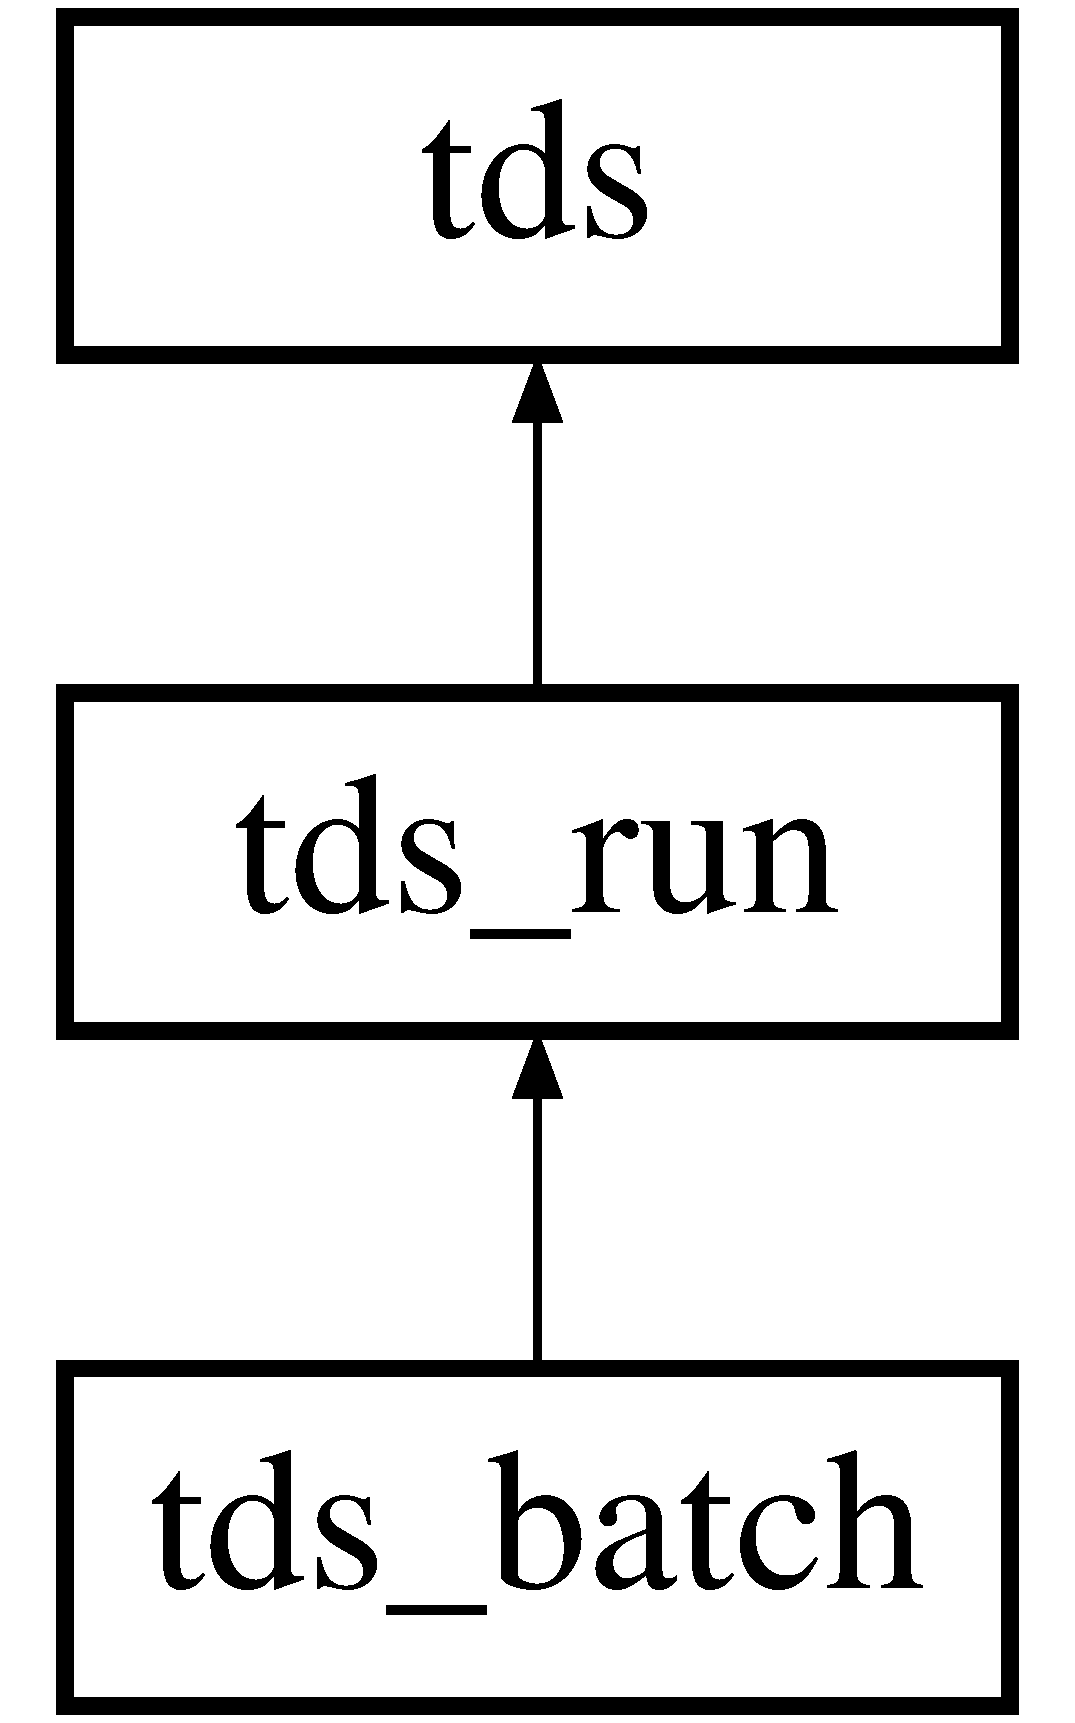
\includegraphics[height=3.000000cm]{classtds__batch}
\end{center}
\end{figure}
\subsection*{Public Member Functions}
\begin{DoxyCompactItemize}
\item 
const char $\ast$ \hyperlink{classtds__batch_a533f64d3586463fb312067fd6902ce17}{rootfile\+\_\+name} ()
\item 
void \hyperlink{classtds__batch_aae27181ea44e97326104535caa34e7e2}{rootfile\+\_\+name} (const char $\ast$\+\_\+rootfile\+\_\+name)
\item 
\hyperlink{classtds__batch_aecd07d1070c0251d5430f17e9ec8b054}{tds\+\_\+batch} (std\+::string infilename, std\+::string rootout)
\item 
virtual \hyperlink{classtds__batch_a198490ee52ed40c59a361f8d86719d72}{$\sim$tds\+\_\+batch} ()
\item 
int \hyperlink{classtds__batch_a09ee988181f4f1b6f2edefced8e617a1}{run\+\_\+batch} (std\+::string filename, bool recreate, int filechain, int n\+\_\+tot)
\item 
std\+::ifstream \& \hyperlink{classtds__batch_a2c311198f8c204dcba09aa413725a895}{inputfile} ()
\end{DoxyCompactItemize}
\subsection*{Additional Inherited Members}


\subsection{Constructor \& Destructor Documentation}
\index{tds\+\_\+batch@{tds\+\_\+batch}!tds\+\_\+batch@{tds\+\_\+batch}}
\index{tds\+\_\+batch@{tds\+\_\+batch}!tds\+\_\+batch@{tds\+\_\+batch}}
\subsubsection[{\texorpdfstring{tds\+\_\+batch(std\+::string infilename, std\+::string rootout)}{tds_batch(std::string infilename, std::string rootout)}}]{\setlength{\rightskip}{0pt plus 5cm}tds\+\_\+batch\+::tds\+\_\+batch (
\begin{DoxyParamCaption}
\item[{std\+::string}]{infilename, }
\item[{std\+::string}]{rootout}
\end{DoxyParamCaption}
)}\hypertarget{classtds__batch_aecd07d1070c0251d5430f17e9ec8b054}{}\label{classtds__batch_aecd07d1070c0251d5430f17e9ec8b054}
\index{tds\+\_\+batch@{tds\+\_\+batch}!````~tds\+\_\+batch@{$\sim$tds\+\_\+batch}}
\index{````~tds\+\_\+batch@{$\sim$tds\+\_\+batch}!tds\+\_\+batch@{tds\+\_\+batch}}
\subsubsection[{\texorpdfstring{$\sim$tds\+\_\+batch()}{~tds_batch()}}]{\setlength{\rightskip}{0pt plus 5cm}tds\+\_\+batch\+::$\sim$tds\+\_\+batch (
\begin{DoxyParamCaption}
{}
\end{DoxyParamCaption}
)\hspace{0.3cm}{\ttfamily [virtual]}}\hypertarget{classtds__batch_a198490ee52ed40c59a361f8d86719d72}{}\label{classtds__batch_a198490ee52ed40c59a361f8d86719d72}


\subsection{Member Function Documentation}
\index{tds\+\_\+batch@{tds\+\_\+batch}!inputfile@{inputfile}}
\index{inputfile@{inputfile}!tds\+\_\+batch@{tds\+\_\+batch}}
\subsubsection[{\texorpdfstring{inputfile()}{inputfile()}}]{\setlength{\rightskip}{0pt plus 5cm}std\+::ifstream\& tds\+\_\+batch\+::inputfile (
\begin{DoxyParamCaption}
{}
\end{DoxyParamCaption}
)\hspace{0.3cm}{\ttfamily [inline]}}\hypertarget{classtds__batch_a2c311198f8c204dcba09aa413725a895}{}\label{classtds__batch_a2c311198f8c204dcba09aa413725a895}
\index{tds\+\_\+batch@{tds\+\_\+batch}!rootfile\+\_\+name@{rootfile\+\_\+name}}
\index{rootfile\+\_\+name@{rootfile\+\_\+name}!tds\+\_\+batch@{tds\+\_\+batch}}
\subsubsection[{\texorpdfstring{rootfile\+\_\+name()}{rootfile_name()}}]{\setlength{\rightskip}{0pt plus 5cm}const char$\ast$ tds\+\_\+batch\+::rootfile\+\_\+name (
\begin{DoxyParamCaption}
{}
\end{DoxyParamCaption}
)\hspace{0.3cm}{\ttfamily [inline]}}\hypertarget{classtds__batch_a533f64d3586463fb312067fd6902ce17}{}\label{classtds__batch_a533f64d3586463fb312067fd6902ce17}
\index{tds\+\_\+batch@{tds\+\_\+batch}!rootfile\+\_\+name@{rootfile\+\_\+name}}
\index{rootfile\+\_\+name@{rootfile\+\_\+name}!tds\+\_\+batch@{tds\+\_\+batch}}
\subsubsection[{\texorpdfstring{rootfile\+\_\+name(const char $\ast$\+\_\+rootfile\+\_\+name)}{rootfile_name(const char *_rootfile_name)}}]{\setlength{\rightskip}{0pt plus 5cm}void tds\+\_\+batch\+::rootfile\+\_\+name (
\begin{DoxyParamCaption}
\item[{const char $\ast$}]{\+\_\+rootfile\+\_\+name}
\end{DoxyParamCaption}
)\hspace{0.3cm}{\ttfamily [inline]}}\hypertarget{classtds__batch_aae27181ea44e97326104535caa34e7e2}{}\label{classtds__batch_aae27181ea44e97326104535caa34e7e2}
\index{tds\+\_\+batch@{tds\+\_\+batch}!run\+\_\+batch@{run\+\_\+batch}}
\index{run\+\_\+batch@{run\+\_\+batch}!tds\+\_\+batch@{tds\+\_\+batch}}
\subsubsection[{\texorpdfstring{run\+\_\+batch(std\+::string filename, bool recreate, int filechain, int n\+\_\+tot)}{run_batch(std::string filename, bool recreate, int filechain, int n_tot)}}]{\setlength{\rightskip}{0pt plus 5cm}int tds\+\_\+batch\+::run\+\_\+batch (
\begin{DoxyParamCaption}
\item[{std\+::string}]{filename, }
\item[{bool}]{recreate, }
\item[{int}]{filechain, }
\item[{int}]{n\+\_\+tot}
\end{DoxyParamCaption}
)}\hypertarget{classtds__batch_a09ee988181f4f1b6f2edefced8e617a1}{}\label{classtds__batch_a09ee988181f4f1b6f2edefced8e617a1}


The documentation for this class was generated from the following files\+:\begin{DoxyCompactItemize}
\item 
\hyperlink{tds_8hh}{tds.\+hh}\item 
\hyperlink{tds_8cc}{tds.\+cc}\end{DoxyCompactItemize}

\hypertarget{classtds__display}{\section{tds\-\_\-display Class Reference}
\label{classtds__display}\index{tds\-\_\-display@{tds\-\_\-display}}
}


{\ttfamily \#include $<$tds.\-hh$>$}

Inheritance diagram for tds\-\_\-display\-:\begin{figure}[H]
\begin{center}
\leavevmode
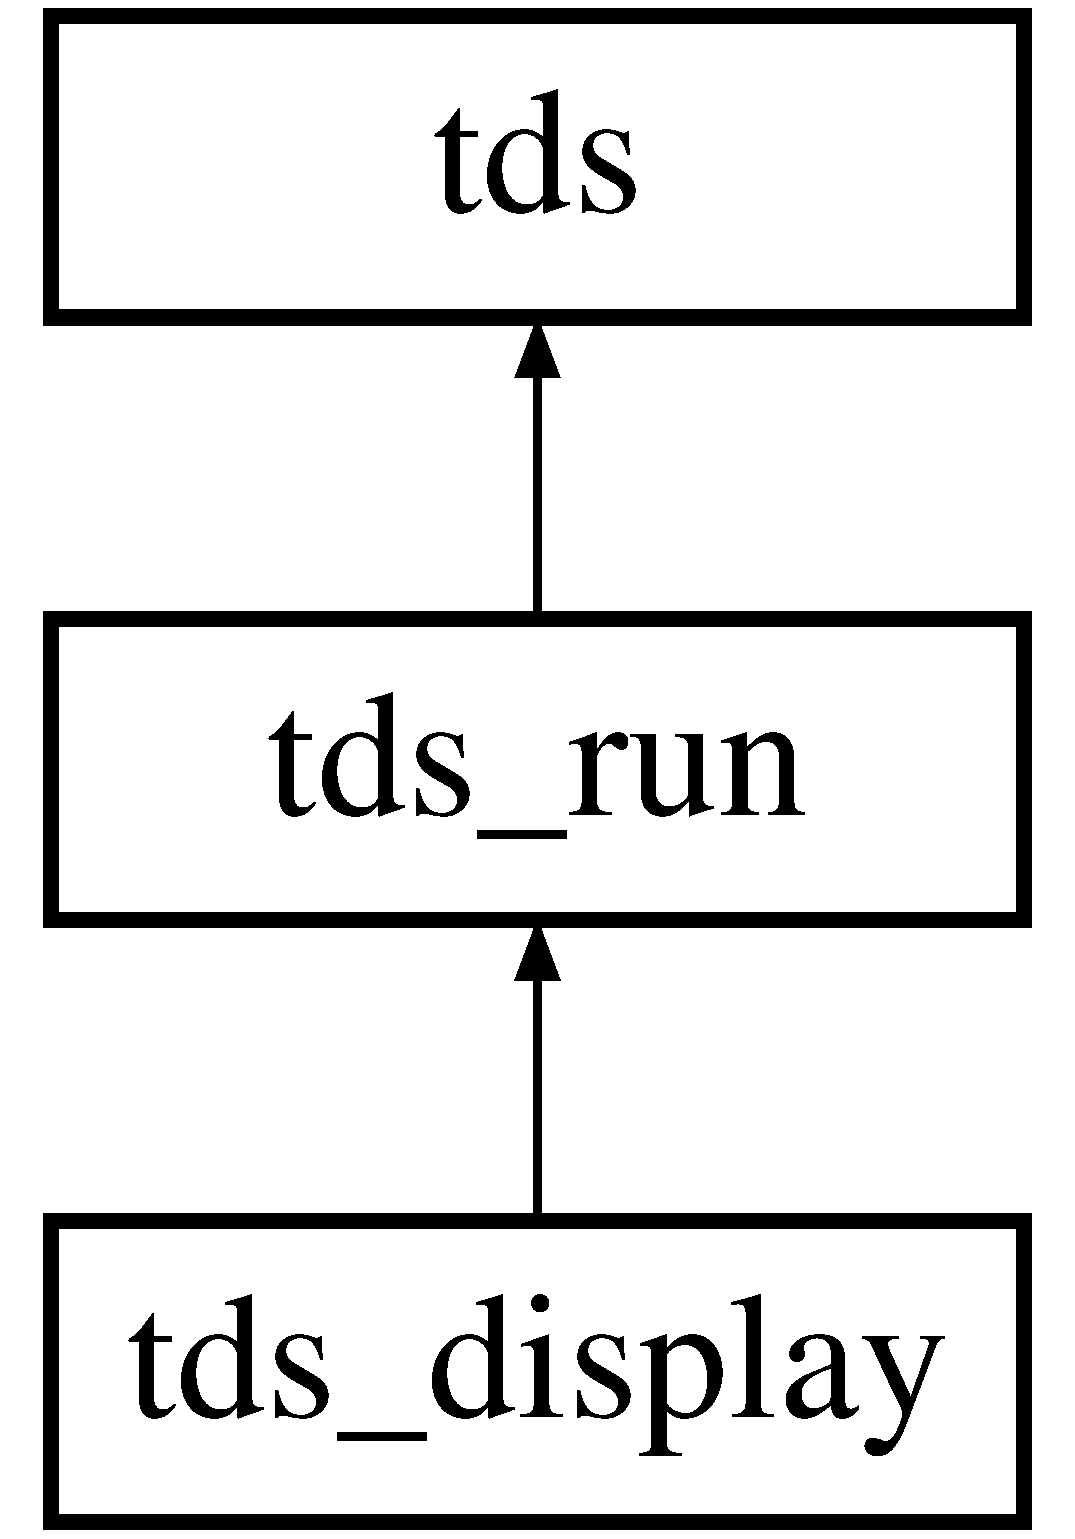
\includegraphics[height=3.000000cm]{classtds__display}
\end{center}
\end{figure}
\subsection*{Public Member Functions}
\begin{DoxyCompactItemize}
\item 
\hyperlink{classtds__display_a4e3eff614025d24fbe8204f98e68b6ce}{tds\-\_\-display} (User\-Interface $\ast$gui)
\item 
virtual \hyperlink{classtds__display_ab31b0f507587abe8aa7acd158e33b0bb}{$\sim$tds\-\_\-display} ()
\item 
User\-Interface \& \hyperlink{classtds__display_ac57fee94adb87f1306e35a3fd1766465}{G\-U\-I} ()
\item 
void \hyperlink{classtds__display_a52823b7451d3afc18eb4a712bb891125}{action} (Fl\-\_\-\-Widget $\ast$sender)
\item 
void \hyperlink{classtds__display_a7135e1577eaab18c500dd503b2b33b0b}{action} (selection sel, Fl\-\_\-\-Widget $\ast$sender)
\item 
void \hyperlink{classtds__display_a86b3c6ef9fe9d846544ce123b325ed40}{plot} ()
\item 
void \hyperlink{classtds__display_a1f5bb8fbcde47a194726ab95aa79e8eb}{display\-\_\-e\-\_\-info} (std\-::string e\-\_\-comment)
\item 
void \hyperlink{classtds__display_ac625020bac2a68d6ab799d37d7b009ea}{display\-\_\-tl\-\_\-info} (std\-::string tl\-\_\-comment)
\item 
void \hyperlink{classtds__display_a188fdc90ab4370b5d1b0b625074ce593}{filename} (const char $\ast$f\-\_\-name)
\item 
std\-::string \hyperlink{classtds__display_aec9a54ceed140fee7120cbf0e7b5d7d8}{display\-\_\-e\-\_\-info} ()
\item 
std\-::string \hyperlink{classtds__display_a1f28ae49914313afc6eb7f218d3cf8bb}{display\-\_\-tl\-\_\-info} ()
\item 
const char $\ast$ \hyperlink{classtds__display_ada7b81a067803aeb6ff761eb9de7a36b}{filename} ()
\end{DoxyCompactItemize}
\subsection*{Protected Member Functions}
\begin{DoxyCompactItemize}
\item 
void \hyperlink{classtds__display_abaaece4e03cb3b0562a57c05bd7e8ef9}{dialog\-\_\-open} ()
\item 
void \hyperlink{classtds__display_ad2289a5a1c2614afbdf9da4fbeea897d}{load\-\_\-event} ()
\item 
void \hyperlink{classtds__display_a6b308b8c7e8b801f07007996e4af2bce}{load\-\_\-section} (int chnum)
\item 
void \hyperlink{classtds__display_a7c7c21140b244d8e3dbfb78aac79e8bc}{load\-\_\-section} (unsigned int c, int chnum)
\item 
void \hyperlink{classtds__display_aad8f138a9fdf0e2e29f70809bd476297}{resize\-\_\-plot} (int \hyperlink{classtds_a09ac79f6931aaf6af64feaca4f167409}{section})
\item 
void \hyperlink{classtds__display_a19c73c213a30b8c1e49f53975fe30341}{make\-Zoom\-Box} (selection sel, int event, int \hyperlink{classtds_a09ac79f6931aaf6af64feaca4f167409}{section})
\end{DoxyCompactItemize}
\subsection*{Additional Inherited Members}


\subsection{Constructor \& Destructor Documentation}
\hypertarget{classtds__display_a4e3eff614025d24fbe8204f98e68b6ce}{\index{tds\-\_\-display@{tds\-\_\-display}!tds\-\_\-display@{tds\-\_\-display}}
\index{tds\-\_\-display@{tds\-\_\-display}!tds_display@{tds\-\_\-display}}
\subsubsection[{tds\-\_\-display}]{\setlength{\rightskip}{0pt plus 5cm}tds\-\_\-display\-::tds\-\_\-display (
\begin{DoxyParamCaption}
\item[{User\-Interface $\ast$}]{gui}
\end{DoxyParamCaption}
)}}\label{classtds__display_a4e3eff614025d24fbe8204f98e68b6ce}
\hypertarget{classtds__display_ab31b0f507587abe8aa7acd158e33b0bb}{\index{tds\-\_\-display@{tds\-\_\-display}!$\sim$tds\-\_\-display@{$\sim$tds\-\_\-display}}
\index{$\sim$tds\-\_\-display@{$\sim$tds\-\_\-display}!tds_display@{tds\-\_\-display}}
\subsubsection[{$\sim$tds\-\_\-display}]{\setlength{\rightskip}{0pt plus 5cm}tds\-\_\-display\-::$\sim$tds\-\_\-display (
\begin{DoxyParamCaption}
{}
\end{DoxyParamCaption}
)\hspace{0.3cm}{\ttfamily [virtual]}}}\label{classtds__display_ab31b0f507587abe8aa7acd158e33b0bb}


\subsection{Member Function Documentation}
\hypertarget{classtds__display_a52823b7451d3afc18eb4a712bb891125}{\index{tds\-\_\-display@{tds\-\_\-display}!action@{action}}
\index{action@{action}!tds_display@{tds\-\_\-display}}
\subsubsection[{action}]{\setlength{\rightskip}{0pt plus 5cm}void tds\-\_\-display\-::action (
\begin{DoxyParamCaption}
\item[{Fl\-\_\-\-Widget $\ast$}]{sender}
\end{DoxyParamCaption}
)}}\label{classtds__display_a52823b7451d3afc18eb4a712bb891125}
\hypertarget{classtds__display_a7135e1577eaab18c500dd503b2b33b0b}{\index{tds\-\_\-display@{tds\-\_\-display}!action@{action}}
\index{action@{action}!tds_display@{tds\-\_\-display}}
\subsubsection[{action}]{\setlength{\rightskip}{0pt plus 5cm}void tds\-\_\-display\-::action (
\begin{DoxyParamCaption}
\item[{selection}]{sel, }
\item[{Fl\-\_\-\-Widget $\ast$}]{sender}
\end{DoxyParamCaption}
)}}\label{classtds__display_a7135e1577eaab18c500dd503b2b33b0b}
\hypertarget{classtds__display_abaaece4e03cb3b0562a57c05bd7e8ef9}{\index{tds\-\_\-display@{tds\-\_\-display}!dialog\-\_\-open@{dialog\-\_\-open}}
\index{dialog\-\_\-open@{dialog\-\_\-open}!tds_display@{tds\-\_\-display}}
\subsubsection[{dialog\-\_\-open}]{\setlength{\rightskip}{0pt plus 5cm}void tds\-\_\-display\-::dialog\-\_\-open (
\begin{DoxyParamCaption}
{}
\end{DoxyParamCaption}
)\hspace{0.3cm}{\ttfamily [protected]}}}\label{classtds__display_abaaece4e03cb3b0562a57c05bd7e8ef9}
\hypertarget{classtds__display_a1f5bb8fbcde47a194726ab95aa79e8eb}{\index{tds\-\_\-display@{tds\-\_\-display}!display\-\_\-e\-\_\-info@{display\-\_\-e\-\_\-info}}
\index{display\-\_\-e\-\_\-info@{display\-\_\-e\-\_\-info}!tds_display@{tds\-\_\-display}}
\subsubsection[{display\-\_\-e\-\_\-info}]{\setlength{\rightskip}{0pt plus 5cm}void tds\-\_\-display\-::display\-\_\-e\-\_\-info (
\begin{DoxyParamCaption}
\item[{std\-::string}]{e\-\_\-comment}
\end{DoxyParamCaption}
)\hspace{0.3cm}{\ttfamily [inline]}}}\label{classtds__display_a1f5bb8fbcde47a194726ab95aa79e8eb}
\hypertarget{classtds__display_aec9a54ceed140fee7120cbf0e7b5d7d8}{\index{tds\-\_\-display@{tds\-\_\-display}!display\-\_\-e\-\_\-info@{display\-\_\-e\-\_\-info}}
\index{display\-\_\-e\-\_\-info@{display\-\_\-e\-\_\-info}!tds_display@{tds\-\_\-display}}
\subsubsection[{display\-\_\-e\-\_\-info}]{\setlength{\rightskip}{0pt plus 5cm}std\-::string tds\-\_\-display\-::display\-\_\-e\-\_\-info (
\begin{DoxyParamCaption}
{}
\end{DoxyParamCaption}
)\hspace{0.3cm}{\ttfamily [inline]}}}\label{classtds__display_aec9a54ceed140fee7120cbf0e7b5d7d8}
\hypertarget{classtds__display_ac625020bac2a68d6ab799d37d7b009ea}{\index{tds\-\_\-display@{tds\-\_\-display}!display\-\_\-tl\-\_\-info@{display\-\_\-tl\-\_\-info}}
\index{display\-\_\-tl\-\_\-info@{display\-\_\-tl\-\_\-info}!tds_display@{tds\-\_\-display}}
\subsubsection[{display\-\_\-tl\-\_\-info}]{\setlength{\rightskip}{0pt plus 5cm}void tds\-\_\-display\-::display\-\_\-tl\-\_\-info (
\begin{DoxyParamCaption}
\item[{std\-::string}]{tl\-\_\-comment}
\end{DoxyParamCaption}
)\hspace{0.3cm}{\ttfamily [inline]}}}\label{classtds__display_ac625020bac2a68d6ab799d37d7b009ea}
\hypertarget{classtds__display_a1f28ae49914313afc6eb7f218d3cf8bb}{\index{tds\-\_\-display@{tds\-\_\-display}!display\-\_\-tl\-\_\-info@{display\-\_\-tl\-\_\-info}}
\index{display\-\_\-tl\-\_\-info@{display\-\_\-tl\-\_\-info}!tds_display@{tds\-\_\-display}}
\subsubsection[{display\-\_\-tl\-\_\-info}]{\setlength{\rightskip}{0pt plus 5cm}std\-::string tds\-\_\-display\-::display\-\_\-tl\-\_\-info (
\begin{DoxyParamCaption}
{}
\end{DoxyParamCaption}
)\hspace{0.3cm}{\ttfamily [inline]}}}\label{classtds__display_a1f28ae49914313afc6eb7f218d3cf8bb}
\hypertarget{classtds__display_a188fdc90ab4370b5d1b0b625074ce593}{\index{tds\-\_\-display@{tds\-\_\-display}!filename@{filename}}
\index{filename@{filename}!tds_display@{tds\-\_\-display}}
\subsubsection[{filename}]{\setlength{\rightskip}{0pt plus 5cm}void tds\-\_\-display\-::filename (
\begin{DoxyParamCaption}
\item[{const char $\ast$}]{f\-\_\-name}
\end{DoxyParamCaption}
)\hspace{0.3cm}{\ttfamily [inline]}}}\label{classtds__display_a188fdc90ab4370b5d1b0b625074ce593}
\hypertarget{classtds__display_ada7b81a067803aeb6ff761eb9de7a36b}{\index{tds\-\_\-display@{tds\-\_\-display}!filename@{filename}}
\index{filename@{filename}!tds_display@{tds\-\_\-display}}
\subsubsection[{filename}]{\setlength{\rightskip}{0pt plus 5cm}const char$\ast$ tds\-\_\-display\-::filename (
\begin{DoxyParamCaption}
{}
\end{DoxyParamCaption}
)\hspace{0.3cm}{\ttfamily [inline]}}}\label{classtds__display_ada7b81a067803aeb6ff761eb9de7a36b}
\hypertarget{classtds__display_ac57fee94adb87f1306e35a3fd1766465}{\index{tds\-\_\-display@{tds\-\_\-display}!G\-U\-I@{G\-U\-I}}
\index{G\-U\-I@{G\-U\-I}!tds_display@{tds\-\_\-display}}
\subsubsection[{G\-U\-I}]{\setlength{\rightskip}{0pt plus 5cm}User\-Interface\& tds\-\_\-display\-::\-G\-U\-I (
\begin{DoxyParamCaption}
{}
\end{DoxyParamCaption}
)\hspace{0.3cm}{\ttfamily [inline]}}}\label{classtds__display_ac57fee94adb87f1306e35a3fd1766465}
\hypertarget{classtds__display_ad2289a5a1c2614afbdf9da4fbeea897d}{\index{tds\-\_\-display@{tds\-\_\-display}!load\-\_\-event@{load\-\_\-event}}
\index{load\-\_\-event@{load\-\_\-event}!tds_display@{tds\-\_\-display}}
\subsubsection[{load\-\_\-event}]{\setlength{\rightskip}{0pt plus 5cm}void tds\-\_\-display\-::load\-\_\-event (
\begin{DoxyParamCaption}
{}
\end{DoxyParamCaption}
)\hspace{0.3cm}{\ttfamily [protected]}}}\label{classtds__display_ad2289a5a1c2614afbdf9da4fbeea897d}
\hypertarget{classtds__display_a6b308b8c7e8b801f07007996e4af2bce}{\index{tds\-\_\-display@{tds\-\_\-display}!load\-\_\-section@{load\-\_\-section}}
\index{load\-\_\-section@{load\-\_\-section}!tds_display@{tds\-\_\-display}}
\subsubsection[{load\-\_\-section}]{\setlength{\rightskip}{0pt plus 5cm}void tds\-\_\-display\-::load\-\_\-section (
\begin{DoxyParamCaption}
\item[{int}]{chnum}
\end{DoxyParamCaption}
)\hspace{0.3cm}{\ttfamily [protected]}}}\label{classtds__display_a6b308b8c7e8b801f07007996e4af2bce}
\hypertarget{classtds__display_a7c7c21140b244d8e3dbfb78aac79e8bc}{\index{tds\-\_\-display@{tds\-\_\-display}!load\-\_\-section@{load\-\_\-section}}
\index{load\-\_\-section@{load\-\_\-section}!tds_display@{tds\-\_\-display}}
\subsubsection[{load\-\_\-section}]{\setlength{\rightskip}{0pt plus 5cm}void tds\-\_\-display\-::load\-\_\-section (
\begin{DoxyParamCaption}
\item[{unsigned int}]{c, }
\item[{int}]{chnum}
\end{DoxyParamCaption}
)\hspace{0.3cm}{\ttfamily [protected]}}}\label{classtds__display_a7c7c21140b244d8e3dbfb78aac79e8bc}
\hypertarget{classtds__display_a19c73c213a30b8c1e49f53975fe30341}{\index{tds\-\_\-display@{tds\-\_\-display}!make\-Zoom\-Box@{make\-Zoom\-Box}}
\index{make\-Zoom\-Box@{make\-Zoom\-Box}!tds_display@{tds\-\_\-display}}
\subsubsection[{make\-Zoom\-Box}]{\setlength{\rightskip}{0pt plus 5cm}void tds\-\_\-display\-::make\-Zoom\-Box (
\begin{DoxyParamCaption}
\item[{selection}]{sel, }
\item[{int}]{event, }
\item[{int}]{section}
\end{DoxyParamCaption}
)\hspace{0.3cm}{\ttfamily [protected]}}}\label{classtds__display_a19c73c213a30b8c1e49f53975fe30341}
\hypertarget{classtds__display_a86b3c6ef9fe9d846544ce123b325ed40}{\index{tds\-\_\-display@{tds\-\_\-display}!plot@{plot}}
\index{plot@{plot}!tds_display@{tds\-\_\-display}}
\subsubsection[{plot}]{\setlength{\rightskip}{0pt plus 5cm}void tds\-\_\-display\-::plot (
\begin{DoxyParamCaption}
{}
\end{DoxyParamCaption}
)}}\label{classtds__display_a86b3c6ef9fe9d846544ce123b325ed40}
\hypertarget{classtds__display_aad8f138a9fdf0e2e29f70809bd476297}{\index{tds\-\_\-display@{tds\-\_\-display}!resize\-\_\-plot@{resize\-\_\-plot}}
\index{resize\-\_\-plot@{resize\-\_\-plot}!tds_display@{tds\-\_\-display}}
\subsubsection[{resize\-\_\-plot}]{\setlength{\rightskip}{0pt plus 5cm}void tds\-\_\-display\-::resize\-\_\-plot (
\begin{DoxyParamCaption}
\item[{int}]{section}
\end{DoxyParamCaption}
)\hspace{0.3cm}{\ttfamily [protected]}}}\label{classtds__display_aad8f138a9fdf0e2e29f70809bd476297}


The documentation for this class was generated from the following files\-:\begin{DoxyCompactItemize}
\item 
\hyperlink{tds_8hh}{tds.\-hh}\item 
\hyperlink{tds_8cc}{tds.\-cc}\end{DoxyCompactItemize}

\hypertarget{classtds__element}{}\section{tds\+\_\+element Class Reference}
\label{classtds__element}\index{tds\+\_\+element@{tds\+\_\+element}}


{\ttfamily \#include $<$tds\+\_\+parts.\+hh$>$}

\subsection*{Public Member Functions}
\begin{DoxyCompactItemize}
\item 
\hyperlink{classtds__element_abcecf7331b6e9eb8901abef93626573d}{tds\+\_\+element} (\hyperlink{tds__parts_8hh_ad445cf91d41fc0e37fcaf259adec00ef}{tds\+\_\+nodes} \+\_\+nodes, \hyperlink{classtds__material}{tds\+\_\+material} $\ast$\+\_\+material, double \+\_\+contamination)
\item 
\hyperlink{classtds__element_aa29190be28bc10a7cc057707532bca21}{tds\+\_\+element} (\hyperlink{tds__parts_8hh_ad445cf91d41fc0e37fcaf259adec00ef}{tds\+\_\+nodes} \+\_\+nodes, \hyperlink{classtds__material}{tds\+\_\+material} $\ast$\+\_\+material, std\+::vector$<$ double $>$ \+\_\+origin, double \+\_\+contamination)
\item 
\hyperlink{classtds__element_acc981290ffd87bad402d32c4508dc5f4}{tds\+\_\+element} (\hyperlink{tds__parts_8hh_ad445cf91d41fc0e37fcaf259adec00ef}{tds\+\_\+nodes} \+\_\+nodes, \hyperlink{classtds__material}{tds\+\_\+material} $\ast$\+\_\+material, double \+\_\+origin\+\_\+x, double \+\_\+origin\+\_\+y, double \+\_\+origin\+\_\+z, double \+\_\+contamination)
\item 
virtual \hyperlink{classtds__element_a209f4917125e72c36d3285980d983892}{$\sim$tds\+\_\+element} ()
\item 
void \hyperlink{classtds__element_a9b3c0e1088fb7ae6da03e8fc1bf9c383}{add\+\_\+element\+\_\+link} (\hyperlink{classtds__element__link}{tds\+\_\+element\+\_\+link} $\ast$new\+\_\+element\+\_\+link)
\item 
void \hyperlink{classtds__element_ab8eb795822ab7e1ea47b703e4f5f473a}{flag\+AB} (bool \+\_\+\+AB)
\item 
void \hyperlink{classtds__element_adb36fa3ae80584e3a4fe12cfdedf6db6}{size} (double \+\_\+size)
\item 
void \hyperlink{classtds__element_a2b3e86e827be59f63cb8d561a73d6983}{contamination} (double \+\_\+contamination)
\item 
void \hyperlink{classtds__element_ae2355a832ead2e50c17a8782ad8d1496}{origin} (double \+\_\+x, double \+\_\+y, double \+\_\+z)
\item 
bool \hyperlink{classtds__element_a44d414a3db34a21320fb70f86f401734}{flag\+AB} ()
\item 
double \hyperlink{classtds__element_a670d658914fce47e7312a170634c47ea}{size} ()
\item 
virtual double \hyperlink{classtds__element_a7dcc7e1ad86d6c64368d1e6215cb662a}{contamination} ()
\item 
virtual double \hyperlink{classtds__element_a5467abfd0fc166336152a668f0f9b67e}{contamination} (bool \+\_\+\+AB)
\item 
double \hyperlink{classtds__element_a737aecedf7dbb0016d0863878f36ca95}{origin} (int i)
\item 
std\+::vector$<$ double $>$ \& \hyperlink{classtds__element_adf1bf79b2b09a06dd6a050cbb90512ce}{origin} ()
\item 
\hyperlink{classtds__material}{tds\+\_\+material} \& \hyperlink{classtds__element_ac06226815fbc171b44a45ef854fe4afd}{material} ()
\item 
\hyperlink{classtds__node}{tds\+\_\+node} \& \hyperlink{classtds__element_a66d829f294782942cf58f6b296f0c3c7}{node} (int i)
\item 
void \hyperlink{classtds__element_a48384c3ca84b54177be7cd67bbc2a5d6}{node} (int i, \hyperlink{classtds__node}{tds\+\_\+node} $\ast$\+\_\+node)
\item 
int \hyperlink{classtds__element_ab79398ce1ba6a67ac5510e44d51b6418}{n\+\_\+nodes} ()
\item 
\hyperlink{classtds__element__link}{tds\+\_\+element\+\_\+link} \& \hyperlink{classtds__element_a83225c7ac9e0577fe9725945319e8783}{neighbour} (int i)
\item 
void \hyperlink{classtds__element_aa14cf978563685ebbf877f6f7518bcb9}{neighbour} (int i, \hyperlink{classtds__element__link}{tds\+\_\+element\+\_\+link} $\ast$\+\_\+element\+\_\+link)
\item 
int \hyperlink{classtds__element_ac41dd60ba9599e0277fe3438f4a2aad0}{n\+\_\+neighbours} ()
\item 
void \hyperlink{classtds__element_ab100134034c37c8c7f6872333cd619f5}{transfer\+\_\+contaminant} (double \+\_\+quantity)
\item 
void \hyperlink{classtds__element_a365817d60d2da273a512db3c8a3a1617}{set\+\_\+origin\+\_\+from\+\_\+nodes} ()
\item 
virtual void \hyperlink{classtds__element_a6c57194ca7f1a73a4bf24e20ba6e56d9}{update} (double delta\+\_\+t)
\item 
void \hyperlink{classtds__element_ae8715ae989c40f56da5fb248afd0e64d}{propogate\+\_\+into\+\_\+nodes} ()
\item 
void \hyperlink{classtds__element_a49f3346e369223a98e405d9dd05569ec}{calculate\+\_\+size} ()
\item 
void \hyperlink{classtds__element_a01868f53394f42b9e437ca6c6a435981}{debug\+\_\+contamination} ()
\item 
bool \hyperlink{classtds__element_a90f1602876bff04b1e3693ebde4ea0a4}{is\+\_\+linked\+\_\+to} (\hyperlink{classtds__element}{tds\+\_\+element} $\ast$\+\_\+element)
\end{DoxyCompactItemize}


\subsection{Constructor \& Destructor Documentation}
\index{tds\+\_\+element@{tds\+\_\+element}!tds\+\_\+element@{tds\+\_\+element}}
\index{tds\+\_\+element@{tds\+\_\+element}!tds\+\_\+element@{tds\+\_\+element}}
\subsubsection[{\texorpdfstring{tds\+\_\+element(tds\+\_\+nodes \+\_\+nodes, tds\+\_\+material $\ast$\+\_\+material, double \+\_\+contamination)}{tds_element(tds_nodes _nodes, tds_material *_material, double _contamination)}}]{\setlength{\rightskip}{0pt plus 5cm}tds\+\_\+element\+::tds\+\_\+element (
\begin{DoxyParamCaption}
\item[{{\bf tds\+\_\+nodes}}]{\+\_\+nodes, }
\item[{{\bf tds\+\_\+material} $\ast$}]{\+\_\+material, }
\item[{double}]{\+\_\+contamination}
\end{DoxyParamCaption}
)}\hypertarget{classtds__element_abcecf7331b6e9eb8901abef93626573d}{}\label{classtds__element_abcecf7331b6e9eb8901abef93626573d}
\index{tds\+\_\+element@{tds\+\_\+element}!tds\+\_\+element@{tds\+\_\+element}}
\index{tds\+\_\+element@{tds\+\_\+element}!tds\+\_\+element@{tds\+\_\+element}}
\subsubsection[{\texorpdfstring{tds\+\_\+element(tds\+\_\+nodes \+\_\+nodes, tds\+\_\+material $\ast$\+\_\+material, std\+::vector$<$ double $>$ \+\_\+origin, double \+\_\+contamination)}{tds_element(tds_nodes _nodes, tds_material *_material, std::vector< double > _origin, double _contamination)}}]{\setlength{\rightskip}{0pt plus 5cm}tds\+\_\+element\+::tds\+\_\+element (
\begin{DoxyParamCaption}
\item[{{\bf tds\+\_\+nodes}}]{\+\_\+nodes, }
\item[{{\bf tds\+\_\+material} $\ast$}]{\+\_\+material, }
\item[{std\+::vector$<$ double $>$}]{\+\_\+origin, }
\item[{double}]{\+\_\+contamination}
\end{DoxyParamCaption}
)}\hypertarget{classtds__element_aa29190be28bc10a7cc057707532bca21}{}\label{classtds__element_aa29190be28bc10a7cc057707532bca21}
\index{tds\+\_\+element@{tds\+\_\+element}!tds\+\_\+element@{tds\+\_\+element}}
\index{tds\+\_\+element@{tds\+\_\+element}!tds\+\_\+element@{tds\+\_\+element}}
\subsubsection[{\texorpdfstring{tds\+\_\+element(tds\+\_\+nodes \+\_\+nodes, tds\+\_\+material $\ast$\+\_\+material, double \+\_\+origin\+\_\+x, double \+\_\+origin\+\_\+y, double \+\_\+origin\+\_\+z, double \+\_\+contamination)}{tds_element(tds_nodes _nodes, tds_material *_material, double _origin_x, double _origin_y, double _origin_z, double _contamination)}}]{\setlength{\rightskip}{0pt plus 5cm}tds\+\_\+element\+::tds\+\_\+element (
\begin{DoxyParamCaption}
\item[{{\bf tds\+\_\+nodes}}]{\+\_\+nodes, }
\item[{{\bf tds\+\_\+material} $\ast$}]{\+\_\+material, }
\item[{double}]{\+\_\+origin\+\_\+x, }
\item[{double}]{\+\_\+origin\+\_\+y, }
\item[{double}]{\+\_\+origin\+\_\+z, }
\item[{double}]{\+\_\+contamination}
\end{DoxyParamCaption}
)}\hypertarget{classtds__element_acc981290ffd87bad402d32c4508dc5f4}{}\label{classtds__element_acc981290ffd87bad402d32c4508dc5f4}
\index{tds\+\_\+element@{tds\+\_\+element}!````~tds\+\_\+element@{$\sim$tds\+\_\+element}}
\index{````~tds\+\_\+element@{$\sim$tds\+\_\+element}!tds\+\_\+element@{tds\+\_\+element}}
\subsubsection[{\texorpdfstring{$\sim$tds\+\_\+element()}{~tds_element()}}]{\setlength{\rightskip}{0pt plus 5cm}tds\+\_\+element\+::$\sim$tds\+\_\+element (
\begin{DoxyParamCaption}
{}
\end{DoxyParamCaption}
)\hspace{0.3cm}{\ttfamily [virtual]}}\hypertarget{classtds__element_a209f4917125e72c36d3285980d983892}{}\label{classtds__element_a209f4917125e72c36d3285980d983892}


\subsection{Member Function Documentation}
\index{tds\+\_\+element@{tds\+\_\+element}!add\+\_\+element\+\_\+link@{add\+\_\+element\+\_\+link}}
\index{add\+\_\+element\+\_\+link@{add\+\_\+element\+\_\+link}!tds\+\_\+element@{tds\+\_\+element}}
\subsubsection[{\texorpdfstring{add\+\_\+element\+\_\+link(tds\+\_\+element\+\_\+link $\ast$new\+\_\+element\+\_\+link)}{add_element_link(tds_element_link *new_element_link)}}]{\setlength{\rightskip}{0pt plus 5cm}void tds\+\_\+element\+::add\+\_\+element\+\_\+link (
\begin{DoxyParamCaption}
\item[{{\bf tds\+\_\+element\+\_\+link} $\ast$}]{new\+\_\+element\+\_\+link}
\end{DoxyParamCaption}
)}\hypertarget{classtds__element_a9b3c0e1088fb7ae6da03e8fc1bf9c383}{}\label{classtds__element_a9b3c0e1088fb7ae6da03e8fc1bf9c383}
\index{tds\+\_\+element@{tds\+\_\+element}!calculate\+\_\+size@{calculate\+\_\+size}}
\index{calculate\+\_\+size@{calculate\+\_\+size}!tds\+\_\+element@{tds\+\_\+element}}
\subsubsection[{\texorpdfstring{calculate\+\_\+size()}{calculate_size()}}]{\setlength{\rightskip}{0pt plus 5cm}void tds\+\_\+element\+::calculate\+\_\+size (
\begin{DoxyParamCaption}
{}
\end{DoxyParamCaption}
)}\hypertarget{classtds__element_a49f3346e369223a98e405d9dd05569ec}{}\label{classtds__element_a49f3346e369223a98e405d9dd05569ec}
\index{tds\+\_\+element@{tds\+\_\+element}!contamination@{contamination}}
\index{contamination@{contamination}!tds\+\_\+element@{tds\+\_\+element}}
\subsubsection[{\texorpdfstring{contamination(double \+\_\+contamination)}{contamination(double _contamination)}}]{\setlength{\rightskip}{0pt plus 5cm}void tds\+\_\+element\+::contamination (
\begin{DoxyParamCaption}
\item[{double}]{\+\_\+contamination}
\end{DoxyParamCaption}
)\hspace{0.3cm}{\ttfamily [inline]}}\hypertarget{classtds__element_a2b3e86e827be59f63cb8d561a73d6983}{}\label{classtds__element_a2b3e86e827be59f63cb8d561a73d6983}
\index{tds\+\_\+element@{tds\+\_\+element}!contamination@{contamination}}
\index{contamination@{contamination}!tds\+\_\+element@{tds\+\_\+element}}
\subsubsection[{\texorpdfstring{contamination()}{contamination()}}]{\setlength{\rightskip}{0pt plus 5cm}virtual double tds\+\_\+element\+::contamination (
\begin{DoxyParamCaption}
{}
\end{DoxyParamCaption}
)\hspace{0.3cm}{\ttfamily [inline]}, {\ttfamily [virtual]}}\hypertarget{classtds__element_a7dcc7e1ad86d6c64368d1e6215cb662a}{}\label{classtds__element_a7dcc7e1ad86d6c64368d1e6215cb662a}
\index{tds\+\_\+element@{tds\+\_\+element}!contamination@{contamination}}
\index{contamination@{contamination}!tds\+\_\+element@{tds\+\_\+element}}
\subsubsection[{\texorpdfstring{contamination(bool \+\_\+\+A\+B)}{contamination(bool _AB)}}]{\setlength{\rightskip}{0pt plus 5cm}virtual double tds\+\_\+element\+::contamination (
\begin{DoxyParamCaption}
\item[{bool}]{\+\_\+\+AB}
\end{DoxyParamCaption}
)\hspace{0.3cm}{\ttfamily [inline]}, {\ttfamily [virtual]}}\hypertarget{classtds__element_a5467abfd0fc166336152a668f0f9b67e}{}\label{classtds__element_a5467abfd0fc166336152a668f0f9b67e}
\index{tds\+\_\+element@{tds\+\_\+element}!debug\+\_\+contamination@{debug\+\_\+contamination}}
\index{debug\+\_\+contamination@{debug\+\_\+contamination}!tds\+\_\+element@{tds\+\_\+element}}
\subsubsection[{\texorpdfstring{debug\+\_\+contamination()}{debug_contamination()}}]{\setlength{\rightskip}{0pt plus 5cm}void tds\+\_\+element\+::debug\+\_\+contamination (
\begin{DoxyParamCaption}
{}
\end{DoxyParamCaption}
)}\hypertarget{classtds__element_a01868f53394f42b9e437ca6c6a435981}{}\label{classtds__element_a01868f53394f42b9e437ca6c6a435981}
\index{tds\+\_\+element@{tds\+\_\+element}!flag\+AB@{flag\+AB}}
\index{flag\+AB@{flag\+AB}!tds\+\_\+element@{tds\+\_\+element}}
\subsubsection[{\texorpdfstring{flag\+A\+B(bool \+\_\+\+A\+B)}{flagAB(bool _AB)}}]{\setlength{\rightskip}{0pt plus 5cm}void tds\+\_\+element\+::flag\+AB (
\begin{DoxyParamCaption}
\item[{bool}]{\+\_\+\+AB}
\end{DoxyParamCaption}
)\hspace{0.3cm}{\ttfamily [inline]}}\hypertarget{classtds__element_ab8eb795822ab7e1ea47b703e4f5f473a}{}\label{classtds__element_ab8eb795822ab7e1ea47b703e4f5f473a}
\index{tds\+\_\+element@{tds\+\_\+element}!flag\+AB@{flag\+AB}}
\index{flag\+AB@{flag\+AB}!tds\+\_\+element@{tds\+\_\+element}}
\subsubsection[{\texorpdfstring{flag\+A\+B()}{flagAB()}}]{\setlength{\rightskip}{0pt plus 5cm}bool tds\+\_\+element\+::flag\+AB (
\begin{DoxyParamCaption}
{}
\end{DoxyParamCaption}
)\hspace{0.3cm}{\ttfamily [inline]}}\hypertarget{classtds__element_a44d414a3db34a21320fb70f86f401734}{}\label{classtds__element_a44d414a3db34a21320fb70f86f401734}
\index{tds\+\_\+element@{tds\+\_\+element}!is\+\_\+linked\+\_\+to@{is\+\_\+linked\+\_\+to}}
\index{is\+\_\+linked\+\_\+to@{is\+\_\+linked\+\_\+to}!tds\+\_\+element@{tds\+\_\+element}}
\subsubsection[{\texorpdfstring{is\+\_\+linked\+\_\+to(tds\+\_\+element $\ast$\+\_\+element)}{is_linked_to(tds_element *_element)}}]{\setlength{\rightskip}{0pt plus 5cm}bool tds\+\_\+element\+::is\+\_\+linked\+\_\+to (
\begin{DoxyParamCaption}
\item[{{\bf tds\+\_\+element} $\ast$}]{\+\_\+element}
\end{DoxyParamCaption}
)}\hypertarget{classtds__element_a90f1602876bff04b1e3693ebde4ea0a4}{}\label{classtds__element_a90f1602876bff04b1e3693ebde4ea0a4}
\index{tds\+\_\+element@{tds\+\_\+element}!material@{material}}
\index{material@{material}!tds\+\_\+element@{tds\+\_\+element}}
\subsubsection[{\texorpdfstring{material()}{material()}}]{\setlength{\rightskip}{0pt plus 5cm}{\bf tds\+\_\+material}\& tds\+\_\+element\+::material (
\begin{DoxyParamCaption}
{}
\end{DoxyParamCaption}
)\hspace{0.3cm}{\ttfamily [inline]}}\hypertarget{classtds__element_ac06226815fbc171b44a45ef854fe4afd}{}\label{classtds__element_ac06226815fbc171b44a45ef854fe4afd}
\index{tds\+\_\+element@{tds\+\_\+element}!n\+\_\+neighbours@{n\+\_\+neighbours}}
\index{n\+\_\+neighbours@{n\+\_\+neighbours}!tds\+\_\+element@{tds\+\_\+element}}
\subsubsection[{\texorpdfstring{n\+\_\+neighbours()}{n_neighbours()}}]{\setlength{\rightskip}{0pt plus 5cm}int tds\+\_\+element\+::n\+\_\+neighbours (
\begin{DoxyParamCaption}
{}
\end{DoxyParamCaption}
)\hspace{0.3cm}{\ttfamily [inline]}}\hypertarget{classtds__element_ac41dd60ba9599e0277fe3438f4a2aad0}{}\label{classtds__element_ac41dd60ba9599e0277fe3438f4a2aad0}
\index{tds\+\_\+element@{tds\+\_\+element}!n\+\_\+nodes@{n\+\_\+nodes}}
\index{n\+\_\+nodes@{n\+\_\+nodes}!tds\+\_\+element@{tds\+\_\+element}}
\subsubsection[{\texorpdfstring{n\+\_\+nodes()}{n_nodes()}}]{\setlength{\rightskip}{0pt plus 5cm}int tds\+\_\+element\+::n\+\_\+nodes (
\begin{DoxyParamCaption}
{}
\end{DoxyParamCaption}
)\hspace{0.3cm}{\ttfamily [inline]}}\hypertarget{classtds__element_ab79398ce1ba6a67ac5510e44d51b6418}{}\label{classtds__element_ab79398ce1ba6a67ac5510e44d51b6418}
\index{tds\+\_\+element@{tds\+\_\+element}!neighbour@{neighbour}}
\index{neighbour@{neighbour}!tds\+\_\+element@{tds\+\_\+element}}
\subsubsection[{\texorpdfstring{neighbour(int i)}{neighbour(int i)}}]{\setlength{\rightskip}{0pt plus 5cm}{\bf tds\+\_\+element\+\_\+link}\& tds\+\_\+element\+::neighbour (
\begin{DoxyParamCaption}
\item[{int}]{i}
\end{DoxyParamCaption}
)\hspace{0.3cm}{\ttfamily [inline]}}\hypertarget{classtds__element_a83225c7ac9e0577fe9725945319e8783}{}\label{classtds__element_a83225c7ac9e0577fe9725945319e8783}
\index{tds\+\_\+element@{tds\+\_\+element}!neighbour@{neighbour}}
\index{neighbour@{neighbour}!tds\+\_\+element@{tds\+\_\+element}}
\subsubsection[{\texorpdfstring{neighbour(int i, tds\+\_\+element\+\_\+link $\ast$\+\_\+element\+\_\+link)}{neighbour(int i, tds_element_link *_element_link)}}]{\setlength{\rightskip}{0pt plus 5cm}void tds\+\_\+element\+::neighbour (
\begin{DoxyParamCaption}
\item[{int}]{i, }
\item[{{\bf tds\+\_\+element\+\_\+link} $\ast$}]{\+\_\+element\+\_\+link}
\end{DoxyParamCaption}
)\hspace{0.3cm}{\ttfamily [inline]}}\hypertarget{classtds__element_aa14cf978563685ebbf877f6f7518bcb9}{}\label{classtds__element_aa14cf978563685ebbf877f6f7518bcb9}
\index{tds\+\_\+element@{tds\+\_\+element}!node@{node}}
\index{node@{node}!tds\+\_\+element@{tds\+\_\+element}}
\subsubsection[{\texorpdfstring{node(int i)}{node(int i)}}]{\setlength{\rightskip}{0pt plus 5cm}{\bf tds\+\_\+node}\& tds\+\_\+element\+::node (
\begin{DoxyParamCaption}
\item[{int}]{i}
\end{DoxyParamCaption}
)\hspace{0.3cm}{\ttfamily [inline]}}\hypertarget{classtds__element_a66d829f294782942cf58f6b296f0c3c7}{}\label{classtds__element_a66d829f294782942cf58f6b296f0c3c7}
\index{tds\+\_\+element@{tds\+\_\+element}!node@{node}}
\index{node@{node}!tds\+\_\+element@{tds\+\_\+element}}
\subsubsection[{\texorpdfstring{node(int i, tds\+\_\+node $\ast$\+\_\+node)}{node(int i, tds_node *_node)}}]{\setlength{\rightskip}{0pt plus 5cm}void tds\+\_\+element\+::node (
\begin{DoxyParamCaption}
\item[{int}]{i, }
\item[{{\bf tds\+\_\+node} $\ast$}]{\+\_\+node}
\end{DoxyParamCaption}
)\hspace{0.3cm}{\ttfamily [inline]}}\hypertarget{classtds__element_a48384c3ca84b54177be7cd67bbc2a5d6}{}\label{classtds__element_a48384c3ca84b54177be7cd67bbc2a5d6}
\index{tds\+\_\+element@{tds\+\_\+element}!origin@{origin}}
\index{origin@{origin}!tds\+\_\+element@{tds\+\_\+element}}
\subsubsection[{\texorpdfstring{origin(double \+\_\+x, double \+\_\+y, double \+\_\+z)}{origin(double _x, double _y, double _z)}}]{\setlength{\rightskip}{0pt plus 5cm}void tds\+\_\+element\+::origin (
\begin{DoxyParamCaption}
\item[{double}]{\+\_\+x, }
\item[{double}]{\+\_\+y, }
\item[{double}]{\+\_\+z}
\end{DoxyParamCaption}
)\hspace{0.3cm}{\ttfamily [inline]}}\hypertarget{classtds__element_ae2355a832ead2e50c17a8782ad8d1496}{}\label{classtds__element_ae2355a832ead2e50c17a8782ad8d1496}
\index{tds\+\_\+element@{tds\+\_\+element}!origin@{origin}}
\index{origin@{origin}!tds\+\_\+element@{tds\+\_\+element}}
\subsubsection[{\texorpdfstring{origin(int i)}{origin(int i)}}]{\setlength{\rightskip}{0pt plus 5cm}double tds\+\_\+element\+::origin (
\begin{DoxyParamCaption}
\item[{int}]{i}
\end{DoxyParamCaption}
)\hspace{0.3cm}{\ttfamily [inline]}}\hypertarget{classtds__element_a737aecedf7dbb0016d0863878f36ca95}{}\label{classtds__element_a737aecedf7dbb0016d0863878f36ca95}
\index{tds\+\_\+element@{tds\+\_\+element}!origin@{origin}}
\index{origin@{origin}!tds\+\_\+element@{tds\+\_\+element}}
\subsubsection[{\texorpdfstring{origin()}{origin()}}]{\setlength{\rightskip}{0pt plus 5cm}std\+::vector$<$double$>$\& tds\+\_\+element\+::origin (
\begin{DoxyParamCaption}
{}
\end{DoxyParamCaption}
)\hspace{0.3cm}{\ttfamily [inline]}}\hypertarget{classtds__element_adf1bf79b2b09a06dd6a050cbb90512ce}{}\label{classtds__element_adf1bf79b2b09a06dd6a050cbb90512ce}
\index{tds\+\_\+element@{tds\+\_\+element}!propogate\+\_\+into\+\_\+nodes@{propogate\+\_\+into\+\_\+nodes}}
\index{propogate\+\_\+into\+\_\+nodes@{propogate\+\_\+into\+\_\+nodes}!tds\+\_\+element@{tds\+\_\+element}}
\subsubsection[{\texorpdfstring{propogate\+\_\+into\+\_\+nodes()}{propogate_into_nodes()}}]{\setlength{\rightskip}{0pt plus 5cm}void tds\+\_\+element\+::propogate\+\_\+into\+\_\+nodes (
\begin{DoxyParamCaption}
{}
\end{DoxyParamCaption}
)}\hypertarget{classtds__element_ae8715ae989c40f56da5fb248afd0e64d}{}\label{classtds__element_ae8715ae989c40f56da5fb248afd0e64d}
\index{tds\+\_\+element@{tds\+\_\+element}!set\+\_\+origin\+\_\+from\+\_\+nodes@{set\+\_\+origin\+\_\+from\+\_\+nodes}}
\index{set\+\_\+origin\+\_\+from\+\_\+nodes@{set\+\_\+origin\+\_\+from\+\_\+nodes}!tds\+\_\+element@{tds\+\_\+element}}
\subsubsection[{\texorpdfstring{set\+\_\+origin\+\_\+from\+\_\+nodes()}{set_origin_from_nodes()}}]{\setlength{\rightskip}{0pt plus 5cm}void tds\+\_\+element\+::set\+\_\+origin\+\_\+from\+\_\+nodes (
\begin{DoxyParamCaption}
{}
\end{DoxyParamCaption}
)}\hypertarget{classtds__element_a365817d60d2da273a512db3c8a3a1617}{}\label{classtds__element_a365817d60d2da273a512db3c8a3a1617}
\index{tds\+\_\+element@{tds\+\_\+element}!size@{size}}
\index{size@{size}!tds\+\_\+element@{tds\+\_\+element}}
\subsubsection[{\texorpdfstring{size(double \+\_\+size)}{size(double _size)}}]{\setlength{\rightskip}{0pt plus 5cm}void tds\+\_\+element\+::size (
\begin{DoxyParamCaption}
\item[{double}]{\+\_\+size}
\end{DoxyParamCaption}
)\hspace{0.3cm}{\ttfamily [inline]}}\hypertarget{classtds__element_adb36fa3ae80584e3a4fe12cfdedf6db6}{}\label{classtds__element_adb36fa3ae80584e3a4fe12cfdedf6db6}
\index{tds\+\_\+element@{tds\+\_\+element}!size@{size}}
\index{size@{size}!tds\+\_\+element@{tds\+\_\+element}}
\subsubsection[{\texorpdfstring{size()}{size()}}]{\setlength{\rightskip}{0pt plus 5cm}double tds\+\_\+element\+::size (
\begin{DoxyParamCaption}
{}
\end{DoxyParamCaption}
)\hspace{0.3cm}{\ttfamily [inline]}}\hypertarget{classtds__element_a670d658914fce47e7312a170634c47ea}{}\label{classtds__element_a670d658914fce47e7312a170634c47ea}
\index{tds\+\_\+element@{tds\+\_\+element}!transfer\+\_\+contaminant@{transfer\+\_\+contaminant}}
\index{transfer\+\_\+contaminant@{transfer\+\_\+contaminant}!tds\+\_\+element@{tds\+\_\+element}}
\subsubsection[{\texorpdfstring{transfer\+\_\+contaminant(double \+\_\+quantity)}{transfer_contaminant(double _quantity)}}]{\setlength{\rightskip}{0pt plus 5cm}void tds\+\_\+element\+::transfer\+\_\+contaminant (
\begin{DoxyParamCaption}
\item[{double}]{\+\_\+quantity}
\end{DoxyParamCaption}
)}\hypertarget{classtds__element_ab100134034c37c8c7f6872333cd619f5}{}\label{classtds__element_ab100134034c37c8c7f6872333cd619f5}
\index{tds\+\_\+element@{tds\+\_\+element}!update@{update}}
\index{update@{update}!tds\+\_\+element@{tds\+\_\+element}}
\subsubsection[{\texorpdfstring{update(double delta\+\_\+t)}{update(double delta_t)}}]{\setlength{\rightskip}{0pt plus 5cm}void tds\+\_\+element\+::update (
\begin{DoxyParamCaption}
\item[{double}]{delta\+\_\+t}
\end{DoxyParamCaption}
)\hspace{0.3cm}{\ttfamily [virtual]}}\hypertarget{classtds__element_a6c57194ca7f1a73a4bf24e20ba6e56d9}{}\label{classtds__element_a6c57194ca7f1a73a4bf24e20ba6e56d9}


The documentation for this class was generated from the following files\+:\begin{DoxyCompactItemize}
\item 
\hyperlink{tds__parts_8hh}{tds\+\_\+parts.\+hh}\item 
\hyperlink{tds__parts_8cc}{tds\+\_\+parts.\+cc}\end{DoxyCompactItemize}

\hypertarget{classtds__element__link}{\section{tds\-\_\-element\-\_\-link Class Reference}
\label{classtds__element__link}\index{tds\-\_\-element\-\_\-link@{tds\-\_\-element\-\_\-link}}
}


{\ttfamily \#include $<$tds\-\_\-parts.\-hh$>$}

Inheritance diagram for tds\-\_\-element\-\_\-link\-:\begin{figure}[H]
\begin{center}
\leavevmode
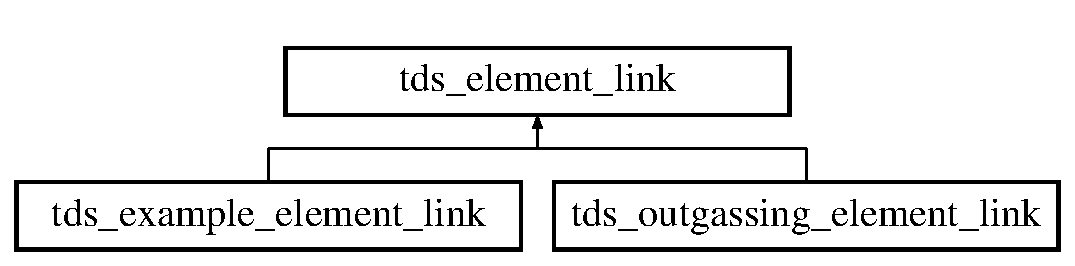
\includegraphics[height=2.000000cm]{classtds__element__link}
\end{center}
\end{figure}
\subsection*{Public Member Functions}
\begin{DoxyCompactItemize}
\item 
\hyperlink{classtds__element__link_a5e72d17aa56494cd0dd7182a0eb87f54}{tds\-\_\-element\-\_\-link} (\hyperlink{classtds__element}{tds\-\_\-element} $\ast$\-\_\-\-M, \hyperlink{classtds__element}{tds\-\_\-element} $\ast$\-\_\-\-N)
\item 
virtual \hyperlink{classtds__element__link_a77a09ccea865dd165d6924a69079df19}{$\sim$tds\-\_\-element\-\_\-link} ()
\item 
void \hyperlink{classtds__element__link_a17a877d4b5b8d4e6ec377bb9ccab4e30}{initialise} ()
\item 
void \hyperlink{classtds__element__link_ad3cf1016587c8d7b9f8417db3459798c}{set\-\_\-flag\-\_\-against} (\hyperlink{classtds__element}{tds\-\_\-element} $\ast$\-\_\-element)
\item 
std\-::vector$<$ double $>$ \& \hyperlink{classtds__element__link_ad8933188624708b7a49f5f7a881f67d8}{norm\-\_\-vector} ()
\item 
double \hyperlink{classtds__element__link_affc5b4d4c6654a65b1067652080b0310}{norm\-\_\-vector} (int i)
\item 
std\-::vector$<$ double $>$ \& \hyperlink{classtds__element__link_ae632fb7dc13fb84791eec31630618101}{flux\-\_\-vector} ()
\item 
double \hyperlink{classtds__element__link_a8d731714b11fd0da48fc7ca2f1ed5f9e}{flux\-\_\-vector} (int i)
\item 
double \hyperlink{classtds__element__link_a024e6be6142af6d8a92263d4a7903389}{interface\-\_\-area} ()
\item 
double \hyperlink{classtds__element__link_acfbf3ede6d850deb4a32c24c958e9a0d}{mod\-M\-N} ()
\item 
double \hyperlink{classtds__element__link_aec8d8d5c53c039dda59aecc430a0f885}{a\-\_\-n\-\_\-dot\-\_\-e\-M\-N\-\_\-over\-\_\-mod\-M\-N} ()
\item 
\hyperlink{classtds__node}{tds\-\_\-node} \& \hyperlink{classtds__element__link_a6c1da2a8aeca0e3d97f0dd02327a0a23}{shared\-\_\-node} (int i)
\item 
\hyperlink{classtds__element}{tds\-\_\-element} \& \hyperlink{classtds__element__link_aa5357b3d1042d36296c67b31eb01e17b}{element\-M} ()
\item 
\hyperlink{classtds__element}{tds\-\_\-element} \& \hyperlink{classtds__element__link_a09a9283ddd611ab673b55c006aefb372}{element\-N} ()
\item 
double \hyperlink{classtds__element__link_a082ea48fa62b672e7ecc5fac8471bcd4}{diffusion\-\_\-constant} ()
\item 
virtual double \hyperlink{classtds__element__link_a2e4a02f2f8cc4941d15734369456f8b7}{flow\-\_\-rate} (bool \-\_\-\-A\-B)
\item 
bool \hyperlink{classtds__element__link_ab3e019113be7a93d6c9ab7faa6350de1}{flag\-A\-B} ()
\item 
short \hyperlink{classtds__element__link_a89ed003b00e4c46416ad7bf3a2d5726e}{positive\-\_\-flow} (\hyperlink{classtds__element}{tds\-\_\-element} $\ast$whoami)
\item 
\hyperlink{classtds__element}{tds\-\_\-element} $\ast$ \hyperlink{classtds__element__link_a4bb693cb080175f184165f5cde55f388}{element} (bool m\-\_\-or\-\_\-n)
\item 
\hyperlink{classtds__element}{tds\-\_\-element} $\ast$ \hyperlink{classtds__element__link_a8c8f17de458d006c051611423a261cfe}{neighbour\-\_\-of} (\hyperlink{classtds__element}{tds\-\_\-element} $\ast$whoami)
\end{DoxyCompactItemize}
\subsection*{Protected Member Functions}
\begin{DoxyCompactItemize}
\item 
void \hyperlink{classtds__element__link_a56039e834e45fba5357a3c10624dc535}{norm\-\_\-vector} (std\-::vector$<$ double $>$ \&\-\_\-norm\-\_\-vector)
\item 
void \hyperlink{classtds__element__link_a4520a07ec97ea614cbc1612f371a55ef}{norm\-\_\-vector} (double \-\_\-x, double \-\_\-y, double \-\_\-z)
\item 
void \hyperlink{classtds__element__link_a2ea4f8a444101e436803d76a2b2420a3}{norm\-\_\-vector} (int i, double \-\_\-f)
\item 
void \hyperlink{classtds__element__link_ad1f6c9650855f5512efb3c6391bba8d3}{flux\-\_\-vector} (std\-::vector$<$ double $>$ \&\-\_\-flux\-\_\-vector)
\item 
void \hyperlink{classtds__element__link_aa013152cdc8496bfb63693d5f1ff934c}{flux\-\_\-vector} (int i, double \-\_\-f)
\item 
void \hyperlink{classtds__element__link_a6a4ed11aefe84f0b9def9fed5da4aa69}{flux\-\_\-vector} (double \-\_\-x, double \-\_\-y, double \-\_\-z)
\item 
void \hyperlink{classtds__element__link_ae49a77335f5a0ae662923a995fc306eb}{interface\-\_\-area} (double \-\_\-area)
\item 
void \hyperlink{classtds__element__link_a7ad521d65162f26fb5b765ed9e3c4292}{mod\-M\-N} (double \-\_\-mod\-M\-N)
\item 
void \hyperlink{classtds__element__link_a9261e32eddd0179b59db7fc705a8b1ce}{a\-\_\-n\-\_\-dot\-\_\-e\-M\-N\-\_\-over\-\_\-mod\-M\-N} (double \-\_\-f)
\item 
void \hyperlink{classtds__element__link_adecad014f5537e295e74290bf6e2bb5c}{flag\-A\-B} (bool \-\_\-\-A\-B)
\end{DoxyCompactItemize}


\subsection{Constructor \& Destructor Documentation}
\hypertarget{classtds__element__link_a5e72d17aa56494cd0dd7182a0eb87f54}{\index{tds\-\_\-element\-\_\-link@{tds\-\_\-element\-\_\-link}!tds\-\_\-element\-\_\-link@{tds\-\_\-element\-\_\-link}}
\index{tds\-\_\-element\-\_\-link@{tds\-\_\-element\-\_\-link}!tds_element_link@{tds\-\_\-element\-\_\-link}}
\subsubsection[{tds\-\_\-element\-\_\-link}]{\setlength{\rightskip}{0pt plus 5cm}tds\-\_\-element\-\_\-link\-::tds\-\_\-element\-\_\-link (
\begin{DoxyParamCaption}
\item[{{\bf tds\-\_\-element} $\ast$}]{\-\_\-\-M, }
\item[{{\bf tds\-\_\-element} $\ast$}]{\-\_\-\-N}
\end{DoxyParamCaption}
)}}\label{classtds__element__link_a5e72d17aa56494cd0dd7182a0eb87f54}
\hypertarget{classtds__element__link_a77a09ccea865dd165d6924a69079df19}{\index{tds\-\_\-element\-\_\-link@{tds\-\_\-element\-\_\-link}!$\sim$tds\-\_\-element\-\_\-link@{$\sim$tds\-\_\-element\-\_\-link}}
\index{$\sim$tds\-\_\-element\-\_\-link@{$\sim$tds\-\_\-element\-\_\-link}!tds_element_link@{tds\-\_\-element\-\_\-link}}
\subsubsection[{$\sim$tds\-\_\-element\-\_\-link}]{\setlength{\rightskip}{0pt plus 5cm}tds\-\_\-element\-\_\-link\-::$\sim$tds\-\_\-element\-\_\-link (
\begin{DoxyParamCaption}
{}
\end{DoxyParamCaption}
)\hspace{0.3cm}{\ttfamily [virtual]}}}\label{classtds__element__link_a77a09ccea865dd165d6924a69079df19}


\subsection{Member Function Documentation}
\hypertarget{classtds__element__link_a9261e32eddd0179b59db7fc705a8b1ce}{\index{tds\-\_\-element\-\_\-link@{tds\-\_\-element\-\_\-link}!a\-\_\-n\-\_\-dot\-\_\-e\-M\-N\-\_\-over\-\_\-mod\-M\-N@{a\-\_\-n\-\_\-dot\-\_\-e\-M\-N\-\_\-over\-\_\-mod\-M\-N}}
\index{a\-\_\-n\-\_\-dot\-\_\-e\-M\-N\-\_\-over\-\_\-mod\-M\-N@{a\-\_\-n\-\_\-dot\-\_\-e\-M\-N\-\_\-over\-\_\-mod\-M\-N}!tds_element_link@{tds\-\_\-element\-\_\-link}}
\subsubsection[{a\-\_\-n\-\_\-dot\-\_\-e\-M\-N\-\_\-over\-\_\-mod\-M\-N}]{\setlength{\rightskip}{0pt plus 5cm}void tds\-\_\-element\-\_\-link\-::a\-\_\-n\-\_\-dot\-\_\-e\-M\-N\-\_\-over\-\_\-mod\-M\-N (
\begin{DoxyParamCaption}
\item[{double}]{\-\_\-f}
\end{DoxyParamCaption}
)\hspace{0.3cm}{\ttfamily [inline]}, {\ttfamily [protected]}}}\label{classtds__element__link_a9261e32eddd0179b59db7fc705a8b1ce}
\hypertarget{classtds__element__link_aec8d8d5c53c039dda59aecc430a0f885}{\index{tds\-\_\-element\-\_\-link@{tds\-\_\-element\-\_\-link}!a\-\_\-n\-\_\-dot\-\_\-e\-M\-N\-\_\-over\-\_\-mod\-M\-N@{a\-\_\-n\-\_\-dot\-\_\-e\-M\-N\-\_\-over\-\_\-mod\-M\-N}}
\index{a\-\_\-n\-\_\-dot\-\_\-e\-M\-N\-\_\-over\-\_\-mod\-M\-N@{a\-\_\-n\-\_\-dot\-\_\-e\-M\-N\-\_\-over\-\_\-mod\-M\-N}!tds_element_link@{tds\-\_\-element\-\_\-link}}
\subsubsection[{a\-\_\-n\-\_\-dot\-\_\-e\-M\-N\-\_\-over\-\_\-mod\-M\-N}]{\setlength{\rightskip}{0pt plus 5cm}double tds\-\_\-element\-\_\-link\-::a\-\_\-n\-\_\-dot\-\_\-e\-M\-N\-\_\-over\-\_\-mod\-M\-N (
\begin{DoxyParamCaption}
{}
\end{DoxyParamCaption}
)\hspace{0.3cm}{\ttfamily [inline]}}}\label{classtds__element__link_aec8d8d5c53c039dda59aecc430a0f885}
\hypertarget{classtds__element__link_a082ea48fa62b672e7ecc5fac8471bcd4}{\index{tds\-\_\-element\-\_\-link@{tds\-\_\-element\-\_\-link}!diffusion\-\_\-constant@{diffusion\-\_\-constant}}
\index{diffusion\-\_\-constant@{diffusion\-\_\-constant}!tds_element_link@{tds\-\_\-element\-\_\-link}}
\subsubsection[{diffusion\-\_\-constant}]{\setlength{\rightskip}{0pt plus 5cm}double tds\-\_\-element\-\_\-link\-::diffusion\-\_\-constant (
\begin{DoxyParamCaption}
{}
\end{DoxyParamCaption}
)}}\label{classtds__element__link_a082ea48fa62b672e7ecc5fac8471bcd4}
\hypertarget{classtds__element__link_a4bb693cb080175f184165f5cde55f388}{\index{tds\-\_\-element\-\_\-link@{tds\-\_\-element\-\_\-link}!element@{element}}
\index{element@{element}!tds_element_link@{tds\-\_\-element\-\_\-link}}
\subsubsection[{element}]{\setlength{\rightskip}{0pt plus 5cm}{\bf tds\-\_\-element}$\ast$ tds\-\_\-element\-\_\-link\-::element (
\begin{DoxyParamCaption}
\item[{bool}]{m\-\_\-or\-\_\-n}
\end{DoxyParamCaption}
)\hspace{0.3cm}{\ttfamily [inline]}}}\label{classtds__element__link_a4bb693cb080175f184165f5cde55f388}
\hypertarget{classtds__element__link_aa5357b3d1042d36296c67b31eb01e17b}{\index{tds\-\_\-element\-\_\-link@{tds\-\_\-element\-\_\-link}!element\-M@{element\-M}}
\index{element\-M@{element\-M}!tds_element_link@{tds\-\_\-element\-\_\-link}}
\subsubsection[{element\-M}]{\setlength{\rightskip}{0pt plus 5cm}{\bf tds\-\_\-element}\& tds\-\_\-element\-\_\-link\-::element\-M (
\begin{DoxyParamCaption}
{}
\end{DoxyParamCaption}
)\hspace{0.3cm}{\ttfamily [inline]}}}\label{classtds__element__link_aa5357b3d1042d36296c67b31eb01e17b}
\hypertarget{classtds__element__link_a09a9283ddd611ab673b55c006aefb372}{\index{tds\-\_\-element\-\_\-link@{tds\-\_\-element\-\_\-link}!element\-N@{element\-N}}
\index{element\-N@{element\-N}!tds_element_link@{tds\-\_\-element\-\_\-link}}
\subsubsection[{element\-N}]{\setlength{\rightskip}{0pt plus 5cm}{\bf tds\-\_\-element}\& tds\-\_\-element\-\_\-link\-::element\-N (
\begin{DoxyParamCaption}
{}
\end{DoxyParamCaption}
)\hspace{0.3cm}{\ttfamily [inline]}}}\label{classtds__element__link_a09a9283ddd611ab673b55c006aefb372}
\hypertarget{classtds__element__link_adecad014f5537e295e74290bf6e2bb5c}{\index{tds\-\_\-element\-\_\-link@{tds\-\_\-element\-\_\-link}!flag\-A\-B@{flag\-A\-B}}
\index{flag\-A\-B@{flag\-A\-B}!tds_element_link@{tds\-\_\-element\-\_\-link}}
\subsubsection[{flag\-A\-B}]{\setlength{\rightskip}{0pt plus 5cm}void tds\-\_\-element\-\_\-link\-::flag\-A\-B (
\begin{DoxyParamCaption}
\item[{bool}]{\-\_\-\-A\-B}
\end{DoxyParamCaption}
)\hspace{0.3cm}{\ttfamily [inline]}, {\ttfamily [protected]}}}\label{classtds__element__link_adecad014f5537e295e74290bf6e2bb5c}
\hypertarget{classtds__element__link_ab3e019113be7a93d6c9ab7faa6350de1}{\index{tds\-\_\-element\-\_\-link@{tds\-\_\-element\-\_\-link}!flag\-A\-B@{flag\-A\-B}}
\index{flag\-A\-B@{flag\-A\-B}!tds_element_link@{tds\-\_\-element\-\_\-link}}
\subsubsection[{flag\-A\-B}]{\setlength{\rightskip}{0pt plus 5cm}bool tds\-\_\-element\-\_\-link\-::flag\-A\-B (
\begin{DoxyParamCaption}
{}
\end{DoxyParamCaption}
)\hspace{0.3cm}{\ttfamily [inline]}}}\label{classtds__element__link_ab3e019113be7a93d6c9ab7faa6350de1}
\hypertarget{classtds__element__link_a2e4a02f2f8cc4941d15734369456f8b7}{\index{tds\-\_\-element\-\_\-link@{tds\-\_\-element\-\_\-link}!flow\-\_\-rate@{flow\-\_\-rate}}
\index{flow\-\_\-rate@{flow\-\_\-rate}!tds_element_link@{tds\-\_\-element\-\_\-link}}
\subsubsection[{flow\-\_\-rate}]{\setlength{\rightskip}{0pt plus 5cm}double tds\-\_\-element\-\_\-link\-::flow\-\_\-rate (
\begin{DoxyParamCaption}
\item[{bool}]{\-\_\-\-A\-B}
\end{DoxyParamCaption}
)\hspace{0.3cm}{\ttfamily [virtual]}}}\label{classtds__element__link_a2e4a02f2f8cc4941d15734369456f8b7}


Reimplemented in \hyperlink{classtds__example__element__link_ab684b4ecbd658f1465a2821a348a51db}{tds\-\_\-example\-\_\-element\-\_\-link}, and \hyperlink{classtds__outgassing__element__link_ad288f7affc2653226877a6c99e242bb3}{tds\-\_\-outgassing\-\_\-element\-\_\-link}.

\hypertarget{classtds__element__link_ad1f6c9650855f5512efb3c6391bba8d3}{\index{tds\-\_\-element\-\_\-link@{tds\-\_\-element\-\_\-link}!flux\-\_\-vector@{flux\-\_\-vector}}
\index{flux\-\_\-vector@{flux\-\_\-vector}!tds_element_link@{tds\-\_\-element\-\_\-link}}
\subsubsection[{flux\-\_\-vector}]{\setlength{\rightskip}{0pt plus 5cm}void tds\-\_\-element\-\_\-link\-::flux\-\_\-vector (
\begin{DoxyParamCaption}
\item[{std\-::vector$<$ double $>$ \&}]{\-\_\-flux\-\_\-vector}
\end{DoxyParamCaption}
)\hspace{0.3cm}{\ttfamily [inline]}, {\ttfamily [protected]}}}\label{classtds__element__link_ad1f6c9650855f5512efb3c6391bba8d3}
\hypertarget{classtds__element__link_aa013152cdc8496bfb63693d5f1ff934c}{\index{tds\-\_\-element\-\_\-link@{tds\-\_\-element\-\_\-link}!flux\-\_\-vector@{flux\-\_\-vector}}
\index{flux\-\_\-vector@{flux\-\_\-vector}!tds_element_link@{tds\-\_\-element\-\_\-link}}
\subsubsection[{flux\-\_\-vector}]{\setlength{\rightskip}{0pt plus 5cm}void tds\-\_\-element\-\_\-link\-::flux\-\_\-vector (
\begin{DoxyParamCaption}
\item[{int}]{i, }
\item[{double}]{\-\_\-f}
\end{DoxyParamCaption}
)\hspace{0.3cm}{\ttfamily [inline]}, {\ttfamily [protected]}}}\label{classtds__element__link_aa013152cdc8496bfb63693d5f1ff934c}
\hypertarget{classtds__element__link_a6a4ed11aefe84f0b9def9fed5da4aa69}{\index{tds\-\_\-element\-\_\-link@{tds\-\_\-element\-\_\-link}!flux\-\_\-vector@{flux\-\_\-vector}}
\index{flux\-\_\-vector@{flux\-\_\-vector}!tds_element_link@{tds\-\_\-element\-\_\-link}}
\subsubsection[{flux\-\_\-vector}]{\setlength{\rightskip}{0pt plus 5cm}void tds\-\_\-element\-\_\-link\-::flux\-\_\-vector (
\begin{DoxyParamCaption}
\item[{double}]{\-\_\-x, }
\item[{double}]{\-\_\-y, }
\item[{double}]{\-\_\-z}
\end{DoxyParamCaption}
)\hspace{0.3cm}{\ttfamily [inline]}, {\ttfamily [protected]}}}\label{classtds__element__link_a6a4ed11aefe84f0b9def9fed5da4aa69}
\hypertarget{classtds__element__link_ae632fb7dc13fb84791eec31630618101}{\index{tds\-\_\-element\-\_\-link@{tds\-\_\-element\-\_\-link}!flux\-\_\-vector@{flux\-\_\-vector}}
\index{flux\-\_\-vector@{flux\-\_\-vector}!tds_element_link@{tds\-\_\-element\-\_\-link}}
\subsubsection[{flux\-\_\-vector}]{\setlength{\rightskip}{0pt plus 5cm}std\-::vector$<$double$>$\& tds\-\_\-element\-\_\-link\-::flux\-\_\-vector (
\begin{DoxyParamCaption}
{}
\end{DoxyParamCaption}
)\hspace{0.3cm}{\ttfamily [inline]}}}\label{classtds__element__link_ae632fb7dc13fb84791eec31630618101}
\hypertarget{classtds__element__link_a8d731714b11fd0da48fc7ca2f1ed5f9e}{\index{tds\-\_\-element\-\_\-link@{tds\-\_\-element\-\_\-link}!flux\-\_\-vector@{flux\-\_\-vector}}
\index{flux\-\_\-vector@{flux\-\_\-vector}!tds_element_link@{tds\-\_\-element\-\_\-link}}
\subsubsection[{flux\-\_\-vector}]{\setlength{\rightskip}{0pt plus 5cm}double tds\-\_\-element\-\_\-link\-::flux\-\_\-vector (
\begin{DoxyParamCaption}
\item[{int}]{i}
\end{DoxyParamCaption}
)\hspace{0.3cm}{\ttfamily [inline]}}}\label{classtds__element__link_a8d731714b11fd0da48fc7ca2f1ed5f9e}
\hypertarget{classtds__element__link_a17a877d4b5b8d4e6ec377bb9ccab4e30}{\index{tds\-\_\-element\-\_\-link@{tds\-\_\-element\-\_\-link}!initialise@{initialise}}
\index{initialise@{initialise}!tds_element_link@{tds\-\_\-element\-\_\-link}}
\subsubsection[{initialise}]{\setlength{\rightskip}{0pt plus 5cm}void tds\-\_\-element\-\_\-link\-::initialise (
\begin{DoxyParamCaption}
{}
\end{DoxyParamCaption}
)}}\label{classtds__element__link_a17a877d4b5b8d4e6ec377bb9ccab4e30}
\hypertarget{classtds__element__link_ae49a77335f5a0ae662923a995fc306eb}{\index{tds\-\_\-element\-\_\-link@{tds\-\_\-element\-\_\-link}!interface\-\_\-area@{interface\-\_\-area}}
\index{interface\-\_\-area@{interface\-\_\-area}!tds_element_link@{tds\-\_\-element\-\_\-link}}
\subsubsection[{interface\-\_\-area}]{\setlength{\rightskip}{0pt plus 5cm}void tds\-\_\-element\-\_\-link\-::interface\-\_\-area (
\begin{DoxyParamCaption}
\item[{double}]{\-\_\-area}
\end{DoxyParamCaption}
)\hspace{0.3cm}{\ttfamily [inline]}, {\ttfamily [protected]}}}\label{classtds__element__link_ae49a77335f5a0ae662923a995fc306eb}
\hypertarget{classtds__element__link_a024e6be6142af6d8a92263d4a7903389}{\index{tds\-\_\-element\-\_\-link@{tds\-\_\-element\-\_\-link}!interface\-\_\-area@{interface\-\_\-area}}
\index{interface\-\_\-area@{interface\-\_\-area}!tds_element_link@{tds\-\_\-element\-\_\-link}}
\subsubsection[{interface\-\_\-area}]{\setlength{\rightskip}{0pt plus 5cm}double tds\-\_\-element\-\_\-link\-::interface\-\_\-area (
\begin{DoxyParamCaption}
{}
\end{DoxyParamCaption}
)\hspace{0.3cm}{\ttfamily [inline]}}}\label{classtds__element__link_a024e6be6142af6d8a92263d4a7903389}
\hypertarget{classtds__element__link_a7ad521d65162f26fb5b765ed9e3c4292}{\index{tds\-\_\-element\-\_\-link@{tds\-\_\-element\-\_\-link}!mod\-M\-N@{mod\-M\-N}}
\index{mod\-M\-N@{mod\-M\-N}!tds_element_link@{tds\-\_\-element\-\_\-link}}
\subsubsection[{mod\-M\-N}]{\setlength{\rightskip}{0pt plus 5cm}void tds\-\_\-element\-\_\-link\-::mod\-M\-N (
\begin{DoxyParamCaption}
\item[{double}]{\-\_\-mod\-M\-N}
\end{DoxyParamCaption}
)\hspace{0.3cm}{\ttfamily [inline]}, {\ttfamily [protected]}}}\label{classtds__element__link_a7ad521d65162f26fb5b765ed9e3c4292}
\hypertarget{classtds__element__link_acfbf3ede6d850deb4a32c24c958e9a0d}{\index{tds\-\_\-element\-\_\-link@{tds\-\_\-element\-\_\-link}!mod\-M\-N@{mod\-M\-N}}
\index{mod\-M\-N@{mod\-M\-N}!tds_element_link@{tds\-\_\-element\-\_\-link}}
\subsubsection[{mod\-M\-N}]{\setlength{\rightskip}{0pt plus 5cm}double tds\-\_\-element\-\_\-link\-::mod\-M\-N (
\begin{DoxyParamCaption}
{}
\end{DoxyParamCaption}
)\hspace{0.3cm}{\ttfamily [inline]}}}\label{classtds__element__link_acfbf3ede6d850deb4a32c24c958e9a0d}
\hypertarget{classtds__element__link_a8c8f17de458d006c051611423a261cfe}{\index{tds\-\_\-element\-\_\-link@{tds\-\_\-element\-\_\-link}!neighbour\-\_\-of@{neighbour\-\_\-of}}
\index{neighbour\-\_\-of@{neighbour\-\_\-of}!tds_element_link@{tds\-\_\-element\-\_\-link}}
\subsubsection[{neighbour\-\_\-of}]{\setlength{\rightskip}{0pt plus 5cm}{\bf tds\-\_\-element}$\ast$ tds\-\_\-element\-\_\-link\-::neighbour\-\_\-of (
\begin{DoxyParamCaption}
\item[{{\bf tds\-\_\-element} $\ast$}]{whoami}
\end{DoxyParamCaption}
)\hspace{0.3cm}{\ttfamily [inline]}}}\label{classtds__element__link_a8c8f17de458d006c051611423a261cfe}
\hypertarget{classtds__element__link_a56039e834e45fba5357a3c10624dc535}{\index{tds\-\_\-element\-\_\-link@{tds\-\_\-element\-\_\-link}!norm\-\_\-vector@{norm\-\_\-vector}}
\index{norm\-\_\-vector@{norm\-\_\-vector}!tds_element_link@{tds\-\_\-element\-\_\-link}}
\subsubsection[{norm\-\_\-vector}]{\setlength{\rightskip}{0pt plus 5cm}void tds\-\_\-element\-\_\-link\-::norm\-\_\-vector (
\begin{DoxyParamCaption}
\item[{std\-::vector$<$ double $>$ \&}]{\-\_\-norm\-\_\-vector}
\end{DoxyParamCaption}
)\hspace{0.3cm}{\ttfamily [inline]}, {\ttfamily [protected]}}}\label{classtds__element__link_a56039e834e45fba5357a3c10624dc535}
\hypertarget{classtds__element__link_a4520a07ec97ea614cbc1612f371a55ef}{\index{tds\-\_\-element\-\_\-link@{tds\-\_\-element\-\_\-link}!norm\-\_\-vector@{norm\-\_\-vector}}
\index{norm\-\_\-vector@{norm\-\_\-vector}!tds_element_link@{tds\-\_\-element\-\_\-link}}
\subsubsection[{norm\-\_\-vector}]{\setlength{\rightskip}{0pt plus 5cm}void tds\-\_\-element\-\_\-link\-::norm\-\_\-vector (
\begin{DoxyParamCaption}
\item[{double}]{\-\_\-x, }
\item[{double}]{\-\_\-y, }
\item[{double}]{\-\_\-z}
\end{DoxyParamCaption}
)\hspace{0.3cm}{\ttfamily [inline]}, {\ttfamily [protected]}}}\label{classtds__element__link_a4520a07ec97ea614cbc1612f371a55ef}
\hypertarget{classtds__element__link_a2ea4f8a444101e436803d76a2b2420a3}{\index{tds\-\_\-element\-\_\-link@{tds\-\_\-element\-\_\-link}!norm\-\_\-vector@{norm\-\_\-vector}}
\index{norm\-\_\-vector@{norm\-\_\-vector}!tds_element_link@{tds\-\_\-element\-\_\-link}}
\subsubsection[{norm\-\_\-vector}]{\setlength{\rightskip}{0pt plus 5cm}void tds\-\_\-element\-\_\-link\-::norm\-\_\-vector (
\begin{DoxyParamCaption}
\item[{int}]{i, }
\item[{double}]{\-\_\-f}
\end{DoxyParamCaption}
)\hspace{0.3cm}{\ttfamily [inline]}, {\ttfamily [protected]}}}\label{classtds__element__link_a2ea4f8a444101e436803d76a2b2420a3}
\hypertarget{classtds__element__link_ad8933188624708b7a49f5f7a881f67d8}{\index{tds\-\_\-element\-\_\-link@{tds\-\_\-element\-\_\-link}!norm\-\_\-vector@{norm\-\_\-vector}}
\index{norm\-\_\-vector@{norm\-\_\-vector}!tds_element_link@{tds\-\_\-element\-\_\-link}}
\subsubsection[{norm\-\_\-vector}]{\setlength{\rightskip}{0pt plus 5cm}std\-::vector$<$double$>$\& tds\-\_\-element\-\_\-link\-::norm\-\_\-vector (
\begin{DoxyParamCaption}
{}
\end{DoxyParamCaption}
)\hspace{0.3cm}{\ttfamily [inline]}}}\label{classtds__element__link_ad8933188624708b7a49f5f7a881f67d8}
\hypertarget{classtds__element__link_affc5b4d4c6654a65b1067652080b0310}{\index{tds\-\_\-element\-\_\-link@{tds\-\_\-element\-\_\-link}!norm\-\_\-vector@{norm\-\_\-vector}}
\index{norm\-\_\-vector@{norm\-\_\-vector}!tds_element_link@{tds\-\_\-element\-\_\-link}}
\subsubsection[{norm\-\_\-vector}]{\setlength{\rightskip}{0pt plus 5cm}double tds\-\_\-element\-\_\-link\-::norm\-\_\-vector (
\begin{DoxyParamCaption}
\item[{int}]{i}
\end{DoxyParamCaption}
)\hspace{0.3cm}{\ttfamily [inline]}}}\label{classtds__element__link_affc5b4d4c6654a65b1067652080b0310}
\hypertarget{classtds__element__link_a89ed003b00e4c46416ad7bf3a2d5726e}{\index{tds\-\_\-element\-\_\-link@{tds\-\_\-element\-\_\-link}!positive\-\_\-flow@{positive\-\_\-flow}}
\index{positive\-\_\-flow@{positive\-\_\-flow}!tds_element_link@{tds\-\_\-element\-\_\-link}}
\subsubsection[{positive\-\_\-flow}]{\setlength{\rightskip}{0pt plus 5cm}short tds\-\_\-element\-\_\-link\-::positive\-\_\-flow (
\begin{DoxyParamCaption}
\item[{{\bf tds\-\_\-element} $\ast$}]{whoami}
\end{DoxyParamCaption}
)\hspace{0.3cm}{\ttfamily [inline]}}}\label{classtds__element__link_a89ed003b00e4c46416ad7bf3a2d5726e}
\hypertarget{classtds__element__link_ad3cf1016587c8d7b9f8417db3459798c}{\index{tds\-\_\-element\-\_\-link@{tds\-\_\-element\-\_\-link}!set\-\_\-flag\-\_\-against@{set\-\_\-flag\-\_\-against}}
\index{set\-\_\-flag\-\_\-against@{set\-\_\-flag\-\_\-against}!tds_element_link@{tds\-\_\-element\-\_\-link}}
\subsubsection[{set\-\_\-flag\-\_\-against}]{\setlength{\rightskip}{0pt plus 5cm}void tds\-\_\-element\-\_\-link\-::set\-\_\-flag\-\_\-against (
\begin{DoxyParamCaption}
\item[{{\bf tds\-\_\-element} $\ast$}]{\-\_\-element}
\end{DoxyParamCaption}
)}}\label{classtds__element__link_ad3cf1016587c8d7b9f8417db3459798c}
\hypertarget{classtds__element__link_a6c1da2a8aeca0e3d97f0dd02327a0a23}{\index{tds\-\_\-element\-\_\-link@{tds\-\_\-element\-\_\-link}!shared\-\_\-node@{shared\-\_\-node}}
\index{shared\-\_\-node@{shared\-\_\-node}!tds_element_link@{tds\-\_\-element\-\_\-link}}
\subsubsection[{shared\-\_\-node}]{\setlength{\rightskip}{0pt plus 5cm}{\bf tds\-\_\-node}\& tds\-\_\-element\-\_\-link\-::shared\-\_\-node (
\begin{DoxyParamCaption}
\item[{int}]{i}
\end{DoxyParamCaption}
)\hspace{0.3cm}{\ttfamily [inline]}}}\label{classtds__element__link_a6c1da2a8aeca0e3d97f0dd02327a0a23}


The documentation for this class was generated from the following files\-:\begin{DoxyCompactItemize}
\item 
\hyperlink{tds__parts_8hh}{tds\-\_\-parts.\-hh}\item 
\hyperlink{tds__parts_8cc}{tds\-\_\-parts.\-cc}\end{DoxyCompactItemize}

\hypertarget{classtds__example__element__link}{\section{tds\-\_\-example\-\_\-element\-\_\-link Class Reference}
\label{classtds__example__element__link}\index{tds\-\_\-example\-\_\-element\-\_\-link@{tds\-\_\-example\-\_\-element\-\_\-link}}
}


{\ttfamily \#include $<$plugin-\/example.\-hh$>$}

Inheritance diagram for tds\-\_\-example\-\_\-element\-\_\-link\-:\begin{figure}[H]
\begin{center}
\leavevmode
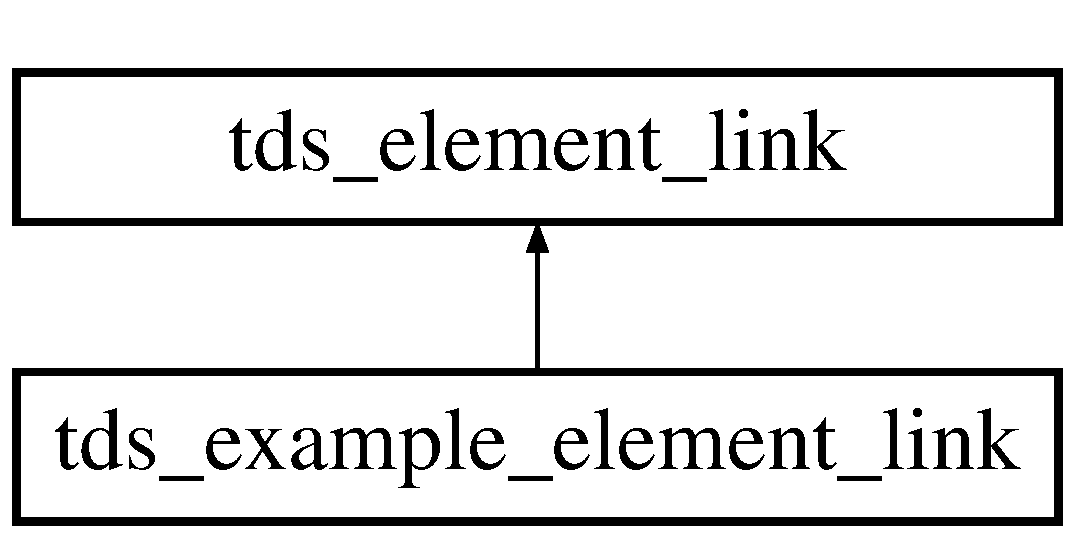
\includegraphics[height=2.000000cm]{classtds__example__element__link}
\end{center}
\end{figure}
\subsection*{Public Member Functions}
\begin{DoxyCompactItemize}
\item 
\hyperlink{classtds__example__element__link_a29ba606b6328d049acc1d099bd60fa13}{tds\-\_\-example\-\_\-element\-\_\-link} (\hyperlink{classtds__element}{tds\-\_\-element} $\ast$\-\_\-\-M, \hyperlink{classtds__element}{tds\-\_\-element} $\ast$\-\_\-\-N)
\item 
double \hyperlink{classtds__example__element__link_ab684b4ecbd658f1465a2821a348a51db}{flow\-\_\-rate} (bool \-\_\-\-A\-B)
\end{DoxyCompactItemize}
\subsection*{Additional Inherited Members}


\subsection{Constructor \& Destructor Documentation}
\hypertarget{classtds__example__element__link_a29ba606b6328d049acc1d099bd60fa13}{\index{tds\-\_\-example\-\_\-element\-\_\-link@{tds\-\_\-example\-\_\-element\-\_\-link}!tds\-\_\-example\-\_\-element\-\_\-link@{tds\-\_\-example\-\_\-element\-\_\-link}}
\index{tds\-\_\-example\-\_\-element\-\_\-link@{tds\-\_\-example\-\_\-element\-\_\-link}!tds_example_element_link@{tds\-\_\-example\-\_\-element\-\_\-link}}
\subsubsection[{tds\-\_\-example\-\_\-element\-\_\-link}]{\setlength{\rightskip}{0pt plus 5cm}tds\-\_\-example\-\_\-element\-\_\-link\-::tds\-\_\-example\-\_\-element\-\_\-link (
\begin{DoxyParamCaption}
\item[{{\bf tds\-\_\-element} $\ast$}]{\-\_\-\-M, }
\item[{{\bf tds\-\_\-element} $\ast$}]{\-\_\-\-N}
\end{DoxyParamCaption}
)}}\label{classtds__example__element__link_a29ba606b6328d049acc1d099bd60fa13}


\subsection{Member Function Documentation}
\hypertarget{classtds__example__element__link_ab684b4ecbd658f1465a2821a348a51db}{\index{tds\-\_\-example\-\_\-element\-\_\-link@{tds\-\_\-example\-\_\-element\-\_\-link}!flow\-\_\-rate@{flow\-\_\-rate}}
\index{flow\-\_\-rate@{flow\-\_\-rate}!tds_example_element_link@{tds\-\_\-example\-\_\-element\-\_\-link}}
\subsubsection[{flow\-\_\-rate}]{\setlength{\rightskip}{0pt plus 5cm}double tds\-\_\-example\-\_\-element\-\_\-link\-::flow\-\_\-rate (
\begin{DoxyParamCaption}
\item[{bool}]{\-\_\-\-A\-B}
\end{DoxyParamCaption}
)\hspace{0.3cm}{\ttfamily [virtual]}}}\label{classtds__example__element__link_ab684b4ecbd658f1465a2821a348a51db}


Reimplemented from \hyperlink{classtds__element__link_a2e4a02f2f8cc4941d15734369456f8b7}{tds\-\_\-element\-\_\-link}.



The documentation for this class was generated from the following files\-:\begin{DoxyCompactItemize}
\item 
\hyperlink{plugin-example_8hh}{plugin-\/example.\-hh}\item 
\hyperlink{plugin-example_8cc}{plugin-\/example.\-cc}\end{DoxyCompactItemize}

\hypertarget{classtds__material}{}\section{tds\+\_\+material Class Reference}
\label{classtds__material}\index{tds\+\_\+material@{tds\+\_\+material}}


{\ttfamily \#include $<$tds\+\_\+parts.\+hh$>$}

\subsection*{Public Member Functions}
\begin{DoxyCompactItemize}
\item 
\hyperlink{classtds__material_af5fb49cd6a56b7eec0bd5c534327c987}{tds\+\_\+material} (std\+::string \+\_\+name, double \+\_\+density, double \+\_\+diffusion\+\_\+constant)
\item 
virtual \hyperlink{classtds__material_ad81f9ebe4bf33e2443479827f7d05b61}{$\sim$tds\+\_\+material} ()
\item 
void \hyperlink{classtds__material_ae1daf38db1671338e414dea7fa97b9f5}{density} (double \+\_\+density)
\item 
void \hyperlink{classtds__material_a26af9e8081aa8bde0fc2eac50b2b6c84}{diffusion\+\_\+constant} (double \+\_\+diffusion\+\_\+constant)
\item 
void \hyperlink{classtds__material_ad3875511cdb690c12fda10b1c8633b61}{material\+\_\+density\+\_\+unit} (std\+::string \+\_\+unit)
\item 
void \hyperlink{classtds__material_a58e27f901a1e39920282b8eb717a26b3}{material\+\_\+diffusion\+\_\+constant\+\_\+unit} (std\+::string \+\_\+unit)
\item 
double \hyperlink{classtds__material_a43ff0d801d23708b91d8ba1dfecb2c42}{density} ()
\item 
double \hyperlink{classtds__material_a8110986dcbebd04a3e80fb8f5eb3d6db}{diffusion\+\_\+constant} ()
\item 
std\+::string \hyperlink{classtds__material_a15016461ba5979216d18999ee7f5095c}{material\+\_\+density\+\_\+unit} ()
\item 
std\+::string \hyperlink{classtds__material_aeba2d3922cb11dc35d21c8951cf8e42e}{material\+\_\+diffusion\+\_\+constant\+\_\+unit} ()
\item 
std\+::string \hyperlink{classtds__material_ab47ac26347c2abeba02060b33db00eeb}{name} ()
\item 
bool \hyperlink{classtds__material_ae35dd97014996e55189b7a0477653639}{is\+\_\+source} ()
\end{DoxyCompactItemize}


\subsection{Constructor \& Destructor Documentation}
\index{tds\+\_\+material@{tds\+\_\+material}!tds\+\_\+material@{tds\+\_\+material}}
\index{tds\+\_\+material@{tds\+\_\+material}!tds\+\_\+material@{tds\+\_\+material}}
\subsubsection[{\texorpdfstring{tds\+\_\+material(std\+::string \+\_\+name, double \+\_\+density, double \+\_\+diffusion\+\_\+constant)}{tds_material(std::string _name, double _density, double _diffusion_constant)}}]{\setlength{\rightskip}{0pt plus 5cm}tds\+\_\+material\+::tds\+\_\+material (
\begin{DoxyParamCaption}
\item[{std\+::string}]{\+\_\+name, }
\item[{double}]{\+\_\+density, }
\item[{double}]{\+\_\+diffusion\+\_\+constant}
\end{DoxyParamCaption}
)}\hypertarget{classtds__material_af5fb49cd6a56b7eec0bd5c534327c987}{}\label{classtds__material_af5fb49cd6a56b7eec0bd5c534327c987}
\index{tds\+\_\+material@{tds\+\_\+material}!````~tds\+\_\+material@{$\sim$tds\+\_\+material}}
\index{````~tds\+\_\+material@{$\sim$tds\+\_\+material}!tds\+\_\+material@{tds\+\_\+material}}
\subsubsection[{\texorpdfstring{$\sim$tds\+\_\+material()}{~tds_material()}}]{\setlength{\rightskip}{0pt plus 5cm}tds\+\_\+material\+::$\sim$tds\+\_\+material (
\begin{DoxyParamCaption}
{}
\end{DoxyParamCaption}
)\hspace{0.3cm}{\ttfamily [virtual]}}\hypertarget{classtds__material_ad81f9ebe4bf33e2443479827f7d05b61}{}\label{classtds__material_ad81f9ebe4bf33e2443479827f7d05b61}


\subsection{Member Function Documentation}
\index{tds\+\_\+material@{tds\+\_\+material}!density@{density}}
\index{density@{density}!tds\+\_\+material@{tds\+\_\+material}}
\subsubsection[{\texorpdfstring{density(double \+\_\+density)}{density(double _density)}}]{\setlength{\rightskip}{0pt plus 5cm}void tds\+\_\+material\+::density (
\begin{DoxyParamCaption}
\item[{double}]{\+\_\+density}
\end{DoxyParamCaption}
)\hspace{0.3cm}{\ttfamily [inline]}}\hypertarget{classtds__material_ae1daf38db1671338e414dea7fa97b9f5}{}\label{classtds__material_ae1daf38db1671338e414dea7fa97b9f5}
\index{tds\+\_\+material@{tds\+\_\+material}!density@{density}}
\index{density@{density}!tds\+\_\+material@{tds\+\_\+material}}
\subsubsection[{\texorpdfstring{density()}{density()}}]{\setlength{\rightskip}{0pt plus 5cm}double tds\+\_\+material\+::density (
\begin{DoxyParamCaption}
{}
\end{DoxyParamCaption}
)\hspace{0.3cm}{\ttfamily [inline]}}\hypertarget{classtds__material_a43ff0d801d23708b91d8ba1dfecb2c42}{}\label{classtds__material_a43ff0d801d23708b91d8ba1dfecb2c42}
\index{tds\+\_\+material@{tds\+\_\+material}!diffusion\+\_\+constant@{diffusion\+\_\+constant}}
\index{diffusion\+\_\+constant@{diffusion\+\_\+constant}!tds\+\_\+material@{tds\+\_\+material}}
\subsubsection[{\texorpdfstring{diffusion\+\_\+constant(double \+\_\+diffusion\+\_\+constant)}{diffusion_constant(double _diffusion_constant)}}]{\setlength{\rightskip}{0pt plus 5cm}void tds\+\_\+material\+::diffusion\+\_\+constant (
\begin{DoxyParamCaption}
\item[{double}]{\+\_\+diffusion\+\_\+constant}
\end{DoxyParamCaption}
)\hspace{0.3cm}{\ttfamily [inline]}}\hypertarget{classtds__material_a26af9e8081aa8bde0fc2eac50b2b6c84}{}\label{classtds__material_a26af9e8081aa8bde0fc2eac50b2b6c84}
\index{tds\+\_\+material@{tds\+\_\+material}!diffusion\+\_\+constant@{diffusion\+\_\+constant}}
\index{diffusion\+\_\+constant@{diffusion\+\_\+constant}!tds\+\_\+material@{tds\+\_\+material}}
\subsubsection[{\texorpdfstring{diffusion\+\_\+constant()}{diffusion_constant()}}]{\setlength{\rightskip}{0pt plus 5cm}double tds\+\_\+material\+::diffusion\+\_\+constant (
\begin{DoxyParamCaption}
{}
\end{DoxyParamCaption}
)\hspace{0.3cm}{\ttfamily [inline]}}\hypertarget{classtds__material_a8110986dcbebd04a3e80fb8f5eb3d6db}{}\label{classtds__material_a8110986dcbebd04a3e80fb8f5eb3d6db}
\index{tds\+\_\+material@{tds\+\_\+material}!is\+\_\+source@{is\+\_\+source}}
\index{is\+\_\+source@{is\+\_\+source}!tds\+\_\+material@{tds\+\_\+material}}
\subsubsection[{\texorpdfstring{is\+\_\+source()}{is_source()}}]{\setlength{\rightskip}{0pt plus 5cm}bool tds\+\_\+material\+::is\+\_\+source (
\begin{DoxyParamCaption}
{}
\end{DoxyParamCaption}
)\hspace{0.3cm}{\ttfamily [inline]}}\hypertarget{classtds__material_ae35dd97014996e55189b7a0477653639}{}\label{classtds__material_ae35dd97014996e55189b7a0477653639}
\index{tds\+\_\+material@{tds\+\_\+material}!material\+\_\+density\+\_\+unit@{material\+\_\+density\+\_\+unit}}
\index{material\+\_\+density\+\_\+unit@{material\+\_\+density\+\_\+unit}!tds\+\_\+material@{tds\+\_\+material}}
\subsubsection[{\texorpdfstring{material\+\_\+density\+\_\+unit(std\+::string \+\_\+unit)}{material_density_unit(std::string _unit)}}]{\setlength{\rightskip}{0pt plus 5cm}void tds\+\_\+material\+::material\+\_\+density\+\_\+unit (
\begin{DoxyParamCaption}
\item[{std\+::string}]{\+\_\+unit}
\end{DoxyParamCaption}
)\hspace{0.3cm}{\ttfamily [inline]}}\hypertarget{classtds__material_ad3875511cdb690c12fda10b1c8633b61}{}\label{classtds__material_ad3875511cdb690c12fda10b1c8633b61}
\index{tds\+\_\+material@{tds\+\_\+material}!material\+\_\+density\+\_\+unit@{material\+\_\+density\+\_\+unit}}
\index{material\+\_\+density\+\_\+unit@{material\+\_\+density\+\_\+unit}!tds\+\_\+material@{tds\+\_\+material}}
\subsubsection[{\texorpdfstring{material\+\_\+density\+\_\+unit()}{material_density_unit()}}]{\setlength{\rightskip}{0pt plus 5cm}std\+::string tds\+\_\+material\+::material\+\_\+density\+\_\+unit (
\begin{DoxyParamCaption}
{}
\end{DoxyParamCaption}
)\hspace{0.3cm}{\ttfamily [inline]}}\hypertarget{classtds__material_a15016461ba5979216d18999ee7f5095c}{}\label{classtds__material_a15016461ba5979216d18999ee7f5095c}
\index{tds\+\_\+material@{tds\+\_\+material}!material\+\_\+diffusion\+\_\+constant\+\_\+unit@{material\+\_\+diffusion\+\_\+constant\+\_\+unit}}
\index{material\+\_\+diffusion\+\_\+constant\+\_\+unit@{material\+\_\+diffusion\+\_\+constant\+\_\+unit}!tds\+\_\+material@{tds\+\_\+material}}
\subsubsection[{\texorpdfstring{material\+\_\+diffusion\+\_\+constant\+\_\+unit(std\+::string \+\_\+unit)}{material_diffusion_constant_unit(std::string _unit)}}]{\setlength{\rightskip}{0pt plus 5cm}void tds\+\_\+material\+::material\+\_\+diffusion\+\_\+constant\+\_\+unit (
\begin{DoxyParamCaption}
\item[{std\+::string}]{\+\_\+unit}
\end{DoxyParamCaption}
)\hspace{0.3cm}{\ttfamily [inline]}}\hypertarget{classtds__material_a58e27f901a1e39920282b8eb717a26b3}{}\label{classtds__material_a58e27f901a1e39920282b8eb717a26b3}
\index{tds\+\_\+material@{tds\+\_\+material}!material\+\_\+diffusion\+\_\+constant\+\_\+unit@{material\+\_\+diffusion\+\_\+constant\+\_\+unit}}
\index{material\+\_\+diffusion\+\_\+constant\+\_\+unit@{material\+\_\+diffusion\+\_\+constant\+\_\+unit}!tds\+\_\+material@{tds\+\_\+material}}
\subsubsection[{\texorpdfstring{material\+\_\+diffusion\+\_\+constant\+\_\+unit()}{material_diffusion_constant_unit()}}]{\setlength{\rightskip}{0pt plus 5cm}std\+::string tds\+\_\+material\+::material\+\_\+diffusion\+\_\+constant\+\_\+unit (
\begin{DoxyParamCaption}
{}
\end{DoxyParamCaption}
)\hspace{0.3cm}{\ttfamily [inline]}}\hypertarget{classtds__material_aeba2d3922cb11dc35d21c8951cf8e42e}{}\label{classtds__material_aeba2d3922cb11dc35d21c8951cf8e42e}
\index{tds\+\_\+material@{tds\+\_\+material}!name@{name}}
\index{name@{name}!tds\+\_\+material@{tds\+\_\+material}}
\subsubsection[{\texorpdfstring{name()}{name()}}]{\setlength{\rightskip}{0pt plus 5cm}std\+::string tds\+\_\+material\+::name (
\begin{DoxyParamCaption}
{}
\end{DoxyParamCaption}
)\hspace{0.3cm}{\ttfamily [inline]}}\hypertarget{classtds__material_ab47ac26347c2abeba02060b33db00eeb}{}\label{classtds__material_ab47ac26347c2abeba02060b33db00eeb}


The documentation for this class was generated from the following files\+:\begin{DoxyCompactItemize}
\item 
\hyperlink{tds__parts_8hh}{tds\+\_\+parts.\+hh}\item 
\hyperlink{tds__parts_8cc}{tds\+\_\+parts.\+cc}\end{DoxyCompactItemize}

\hypertarget{classtds__node}{\section{tds\-\_\-node Class Reference}
\label{classtds__node}\index{tds\-\_\-node@{tds\-\_\-node}}
}


{\ttfamily \#include $<$tds\-\_\-parts.\-hh$>$}

\subsection*{Public Member Functions}
\begin{DoxyCompactItemize}
\item 
\hyperlink{classtds__node_aae4e896d901f88ab725df449454412e4}{tds\-\_\-node} (double \-\_\-x, double \-\_\-y, double \-\_\-z)
\item 
\hyperlink{classtds__node_ad485694533fbe32047035cf9c4ffca48}{tds\-\_\-node} (std\-::vector$<$ double $>$ \-\_\-position)
\item 
\hyperlink{classtds__node_afd27a4e35834832cb923db673ee4b3ee}{$\sim$tds\-\_\-node} ()
\item 
void \hyperlink{classtds__node_a678be3112890f9998796c2c7033e2e91}{add\-\_\-element} (\hyperlink{classtds__element}{tds\-\_\-element} $\ast$new\-\_\-element)
\item 
void \hyperlink{classtds__node_a6967a1b6824ff0cb64c901746994a9a2}{position} (std\-::vector$<$ double $>$ \-\_\-position)
\item 
void \hyperlink{classtds__node_a8cf9300cdb4b20bbebf9a2f04b37695f}{position} (int i, double \-\_\-p)
\item 
std\-::vector$<$ double $>$ \hyperlink{classtds__node_ac4fbb78ffb5d7c27384c9ca0bb16f39e}{position} ()
\item 
double \hyperlink{classtds__node_ab9fc6244a5657f8bd6eaea8bf86f0346}{position} (int i)
\item 
\hyperlink{classtds__element}{tds\-\_\-element} \& \hyperlink{classtds__node_ae0efbd59681b496e53ee685e1b7d59a6}{element} (int i)
\item 
void \hyperlink{classtds__node_a9d329513511f86cc828792e4eff4c3e7}{element} (int i, \hyperlink{classtds__element}{tds\-\_\-element} $\ast$\-\_\-new\-\_\-element)
\item 
bool \hyperlink{classtds__node_a285d91e52abf56986f50a91e615cf9f5}{elements\-\_\-empty} ()
\item 
int \hyperlink{classtds__node_a4066ea71ef3ea4329c82aef6ee0ff41a}{n\-\_\-elements} ()
\item 
void \hyperlink{classtds__node_a7fd1af280d8db87fa3a1c4942f54420c}{clean\-\_\-elements} ()
\item 
void \hyperlink{classtds__node_a9659601fc4789ccaad501018f864dc2a}{remove\-\_\-last\-\_\-element} ()
\end{DoxyCompactItemize}


\subsection{Constructor \& Destructor Documentation}
\hypertarget{classtds__node_aae4e896d901f88ab725df449454412e4}{\index{tds\-\_\-node@{tds\-\_\-node}!tds\-\_\-node@{tds\-\_\-node}}
\index{tds\-\_\-node@{tds\-\_\-node}!tds_node@{tds\-\_\-node}}
\subsubsection[{tds\-\_\-node}]{\setlength{\rightskip}{0pt plus 5cm}tds\-\_\-node\-::tds\-\_\-node (
\begin{DoxyParamCaption}
\item[{double}]{\-\_\-x, }
\item[{double}]{\-\_\-y, }
\item[{double}]{\-\_\-z}
\end{DoxyParamCaption}
)}}\label{classtds__node_aae4e896d901f88ab725df449454412e4}
\hypertarget{classtds__node_ad485694533fbe32047035cf9c4ffca48}{\index{tds\-\_\-node@{tds\-\_\-node}!tds\-\_\-node@{tds\-\_\-node}}
\index{tds\-\_\-node@{tds\-\_\-node}!tds_node@{tds\-\_\-node}}
\subsubsection[{tds\-\_\-node}]{\setlength{\rightskip}{0pt plus 5cm}tds\-\_\-node\-::tds\-\_\-node (
\begin{DoxyParamCaption}
\item[{std\-::vector$<$ double $>$}]{\-\_\-position}
\end{DoxyParamCaption}
)}}\label{classtds__node_ad485694533fbe32047035cf9c4ffca48}
\hypertarget{classtds__node_afd27a4e35834832cb923db673ee4b3ee}{\index{tds\-\_\-node@{tds\-\_\-node}!$\sim$tds\-\_\-node@{$\sim$tds\-\_\-node}}
\index{$\sim$tds\-\_\-node@{$\sim$tds\-\_\-node}!tds_node@{tds\-\_\-node}}
\subsubsection[{$\sim$tds\-\_\-node}]{\setlength{\rightskip}{0pt plus 5cm}tds\-\_\-node\-::$\sim$tds\-\_\-node (
\begin{DoxyParamCaption}
{}
\end{DoxyParamCaption}
)}}\label{classtds__node_afd27a4e35834832cb923db673ee4b3ee}


\subsection{Member Function Documentation}
\hypertarget{classtds__node_a678be3112890f9998796c2c7033e2e91}{\index{tds\-\_\-node@{tds\-\_\-node}!add\-\_\-element@{add\-\_\-element}}
\index{add\-\_\-element@{add\-\_\-element}!tds_node@{tds\-\_\-node}}
\subsubsection[{add\-\_\-element}]{\setlength{\rightskip}{0pt plus 5cm}void tds\-\_\-node\-::add\-\_\-element (
\begin{DoxyParamCaption}
\item[{{\bf tds\-\_\-element} $\ast$}]{new\-\_\-element}
\end{DoxyParamCaption}
)}}\label{classtds__node_a678be3112890f9998796c2c7033e2e91}
\hypertarget{classtds__node_a7fd1af280d8db87fa3a1c4942f54420c}{\index{tds\-\_\-node@{tds\-\_\-node}!clean\-\_\-elements@{clean\-\_\-elements}}
\index{clean\-\_\-elements@{clean\-\_\-elements}!tds_node@{tds\-\_\-node}}
\subsubsection[{clean\-\_\-elements}]{\setlength{\rightskip}{0pt plus 5cm}void tds\-\_\-node\-::clean\-\_\-elements (
\begin{DoxyParamCaption}
{}
\end{DoxyParamCaption}
)}}\label{classtds__node_a7fd1af280d8db87fa3a1c4942f54420c}
\hypertarget{classtds__node_ae0efbd59681b496e53ee685e1b7d59a6}{\index{tds\-\_\-node@{tds\-\_\-node}!element@{element}}
\index{element@{element}!tds_node@{tds\-\_\-node}}
\subsubsection[{element}]{\setlength{\rightskip}{0pt plus 5cm}{\bf tds\-\_\-element}\& tds\-\_\-node\-::element (
\begin{DoxyParamCaption}
\item[{int}]{i}
\end{DoxyParamCaption}
)\hspace{0.3cm}{\ttfamily [inline]}}}\label{classtds__node_ae0efbd59681b496e53ee685e1b7d59a6}
\hypertarget{classtds__node_a9d329513511f86cc828792e4eff4c3e7}{\index{tds\-\_\-node@{tds\-\_\-node}!element@{element}}
\index{element@{element}!tds_node@{tds\-\_\-node}}
\subsubsection[{element}]{\setlength{\rightskip}{0pt plus 5cm}void tds\-\_\-node\-::element (
\begin{DoxyParamCaption}
\item[{int}]{i, }
\item[{{\bf tds\-\_\-element} $\ast$}]{\-\_\-new\-\_\-element}
\end{DoxyParamCaption}
)\hspace{0.3cm}{\ttfamily [inline]}}}\label{classtds__node_a9d329513511f86cc828792e4eff4c3e7}
\hypertarget{classtds__node_a285d91e52abf56986f50a91e615cf9f5}{\index{tds\-\_\-node@{tds\-\_\-node}!elements\-\_\-empty@{elements\-\_\-empty}}
\index{elements\-\_\-empty@{elements\-\_\-empty}!tds_node@{tds\-\_\-node}}
\subsubsection[{elements\-\_\-empty}]{\setlength{\rightskip}{0pt plus 5cm}bool tds\-\_\-node\-::elements\-\_\-empty (
\begin{DoxyParamCaption}
{}
\end{DoxyParamCaption}
)\hspace{0.3cm}{\ttfamily [inline]}}}\label{classtds__node_a285d91e52abf56986f50a91e615cf9f5}
\hypertarget{classtds__node_a4066ea71ef3ea4329c82aef6ee0ff41a}{\index{tds\-\_\-node@{tds\-\_\-node}!n\-\_\-elements@{n\-\_\-elements}}
\index{n\-\_\-elements@{n\-\_\-elements}!tds_node@{tds\-\_\-node}}
\subsubsection[{n\-\_\-elements}]{\setlength{\rightskip}{0pt plus 5cm}int tds\-\_\-node\-::n\-\_\-elements (
\begin{DoxyParamCaption}
{}
\end{DoxyParamCaption}
)\hspace{0.3cm}{\ttfamily [inline]}}}\label{classtds__node_a4066ea71ef3ea4329c82aef6ee0ff41a}
\hypertarget{classtds__node_a6967a1b6824ff0cb64c901746994a9a2}{\index{tds\-\_\-node@{tds\-\_\-node}!position@{position}}
\index{position@{position}!tds_node@{tds\-\_\-node}}
\subsubsection[{position}]{\setlength{\rightskip}{0pt plus 5cm}void tds\-\_\-node\-::position (
\begin{DoxyParamCaption}
\item[{std\-::vector$<$ double $>$}]{\-\_\-position}
\end{DoxyParamCaption}
)\hspace{0.3cm}{\ttfamily [inline]}}}\label{classtds__node_a6967a1b6824ff0cb64c901746994a9a2}
\hypertarget{classtds__node_a8cf9300cdb4b20bbebf9a2f04b37695f}{\index{tds\-\_\-node@{tds\-\_\-node}!position@{position}}
\index{position@{position}!tds_node@{tds\-\_\-node}}
\subsubsection[{position}]{\setlength{\rightskip}{0pt plus 5cm}void tds\-\_\-node\-::position (
\begin{DoxyParamCaption}
\item[{int}]{i, }
\item[{double}]{\-\_\-p}
\end{DoxyParamCaption}
)\hspace{0.3cm}{\ttfamily [inline]}}}\label{classtds__node_a8cf9300cdb4b20bbebf9a2f04b37695f}
\hypertarget{classtds__node_ac4fbb78ffb5d7c27384c9ca0bb16f39e}{\index{tds\-\_\-node@{tds\-\_\-node}!position@{position}}
\index{position@{position}!tds_node@{tds\-\_\-node}}
\subsubsection[{position}]{\setlength{\rightskip}{0pt plus 5cm}std\-::vector$<$double$>$ tds\-\_\-node\-::position (
\begin{DoxyParamCaption}
{}
\end{DoxyParamCaption}
)\hspace{0.3cm}{\ttfamily [inline]}}}\label{classtds__node_ac4fbb78ffb5d7c27384c9ca0bb16f39e}
\hypertarget{classtds__node_ab9fc6244a5657f8bd6eaea8bf86f0346}{\index{tds\-\_\-node@{tds\-\_\-node}!position@{position}}
\index{position@{position}!tds_node@{tds\-\_\-node}}
\subsubsection[{position}]{\setlength{\rightskip}{0pt plus 5cm}double tds\-\_\-node\-::position (
\begin{DoxyParamCaption}
\item[{int}]{i}
\end{DoxyParamCaption}
)\hspace{0.3cm}{\ttfamily [inline]}}}\label{classtds__node_ab9fc6244a5657f8bd6eaea8bf86f0346}
\hypertarget{classtds__node_a9659601fc4789ccaad501018f864dc2a}{\index{tds\-\_\-node@{tds\-\_\-node}!remove\-\_\-last\-\_\-element@{remove\-\_\-last\-\_\-element}}
\index{remove\-\_\-last\-\_\-element@{remove\-\_\-last\-\_\-element}!tds_node@{tds\-\_\-node}}
\subsubsection[{remove\-\_\-last\-\_\-element}]{\setlength{\rightskip}{0pt plus 5cm}void tds\-\_\-node\-::remove\-\_\-last\-\_\-element (
\begin{DoxyParamCaption}
{}
\end{DoxyParamCaption}
)}}\label{classtds__node_a9659601fc4789ccaad501018f864dc2a}


The documentation for this class was generated from the following files\-:\begin{DoxyCompactItemize}
\item 
\hyperlink{tds__parts_8hh}{tds\-\_\-parts.\-hh}\item 
\hyperlink{tds__parts_8cc}{tds\-\_\-parts.\-cc}\end{DoxyCompactItemize}

\hypertarget{classtds__outgassing__element__link}{\section{tds\-\_\-outgassing\-\_\-element\-\_\-link Class Reference}
\label{classtds__outgassing__element__link}\index{tds\-\_\-outgassing\-\_\-element\-\_\-link@{tds\-\_\-outgassing\-\_\-element\-\_\-link}}
}


{\ttfamily \#include $<$plugin-\/outgassing.\-hh$>$}

Inheritance diagram for tds\-\_\-outgassing\-\_\-element\-\_\-link\-:\begin{figure}[H]
\begin{center}
\leavevmode
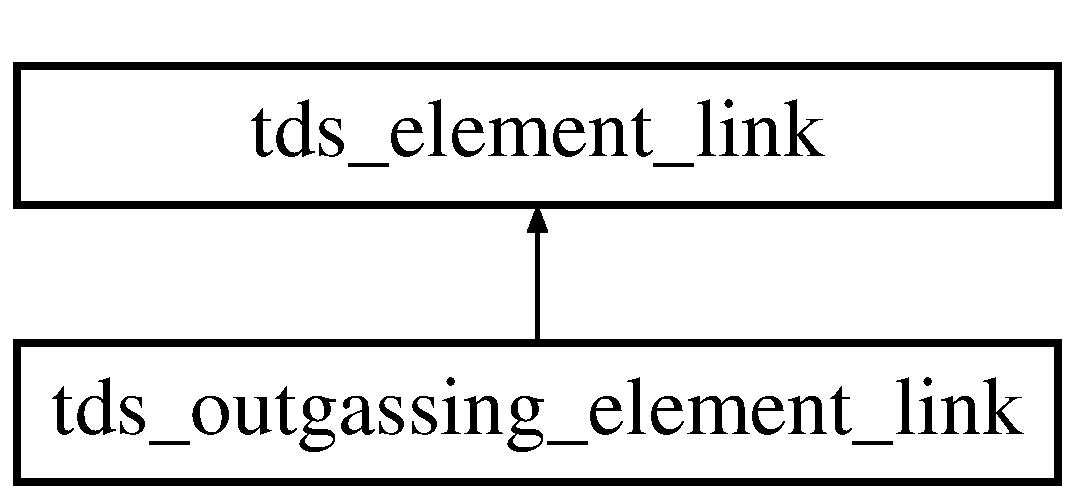
\includegraphics[height=2.000000cm]{classtds__outgassing__element__link}
\end{center}
\end{figure}
\subsection*{Public Member Functions}
\begin{DoxyCompactItemize}
\item 
\hyperlink{classtds__outgassing__element__link_a21b525492ecf1ef4ea45168be8c2961c}{tds\-\_\-outgassing\-\_\-element\-\_\-link} (\hyperlink{classtds__element}{tds\-\_\-element} $\ast$\-\_\-\-M, \hyperlink{classtds__element}{tds\-\_\-element} $\ast$\-\_\-\-N)
\item 
double \hyperlink{classtds__outgassing__element__link_ad288f7affc2653226877a6c99e242bb3}{flow\-\_\-rate} (bool \-\_\-\-A\-B)
\end{DoxyCompactItemize}
\subsection*{Additional Inherited Members}


\subsection{Constructor \& Destructor Documentation}
\hypertarget{classtds__outgassing__element__link_a21b525492ecf1ef4ea45168be8c2961c}{\index{tds\-\_\-outgassing\-\_\-element\-\_\-link@{tds\-\_\-outgassing\-\_\-element\-\_\-link}!tds\-\_\-outgassing\-\_\-element\-\_\-link@{tds\-\_\-outgassing\-\_\-element\-\_\-link}}
\index{tds\-\_\-outgassing\-\_\-element\-\_\-link@{tds\-\_\-outgassing\-\_\-element\-\_\-link}!tds_outgassing_element_link@{tds\-\_\-outgassing\-\_\-element\-\_\-link}}
\subsubsection[{tds\-\_\-outgassing\-\_\-element\-\_\-link}]{\setlength{\rightskip}{0pt plus 5cm}tds\-\_\-outgassing\-\_\-element\-\_\-link\-::tds\-\_\-outgassing\-\_\-element\-\_\-link (
\begin{DoxyParamCaption}
\item[{{\bf tds\-\_\-element} $\ast$}]{\-\_\-\-M, }
\item[{{\bf tds\-\_\-element} $\ast$}]{\-\_\-\-N}
\end{DoxyParamCaption}
)}}\label{classtds__outgassing__element__link_a21b525492ecf1ef4ea45168be8c2961c}


\subsection{Member Function Documentation}
\hypertarget{classtds__outgassing__element__link_ad288f7affc2653226877a6c99e242bb3}{\index{tds\-\_\-outgassing\-\_\-element\-\_\-link@{tds\-\_\-outgassing\-\_\-element\-\_\-link}!flow\-\_\-rate@{flow\-\_\-rate}}
\index{flow\-\_\-rate@{flow\-\_\-rate}!tds_outgassing_element_link@{tds\-\_\-outgassing\-\_\-element\-\_\-link}}
\subsubsection[{flow\-\_\-rate}]{\setlength{\rightskip}{0pt plus 5cm}double tds\-\_\-outgassing\-\_\-element\-\_\-link\-::flow\-\_\-rate (
\begin{DoxyParamCaption}
\item[{bool}]{\-\_\-\-A\-B}
\end{DoxyParamCaption}
)\hspace{0.3cm}{\ttfamily [virtual]}}}\label{classtds__outgassing__element__link_ad288f7affc2653226877a6c99e242bb3}


Reimplemented from \hyperlink{classtds__element__link_a2e4a02f2f8cc4941d15734369456f8b7}{tds\-\_\-element\-\_\-link}.



The documentation for this class was generated from the following files\-:\begin{DoxyCompactItemize}
\item 
\hyperlink{plugin-outgassing_8hh}{plugin-\/outgassing.\-hh}\item 
\hyperlink{plugin-outgassing_8cc}{plugin-\/outgassing.\-cc}\end{DoxyCompactItemize}

\hypertarget{classtds__run}{}\section{tds\+\_\+run Class Reference}
\label{classtds__run}\index{tds\+\_\+run@{tds\+\_\+run}}


{\ttfamily \#include $<$tds.\+hh$>$}

Inheritance diagram for tds\+\_\+run\+:\begin{figure}[H]
\begin{center}
\leavevmode
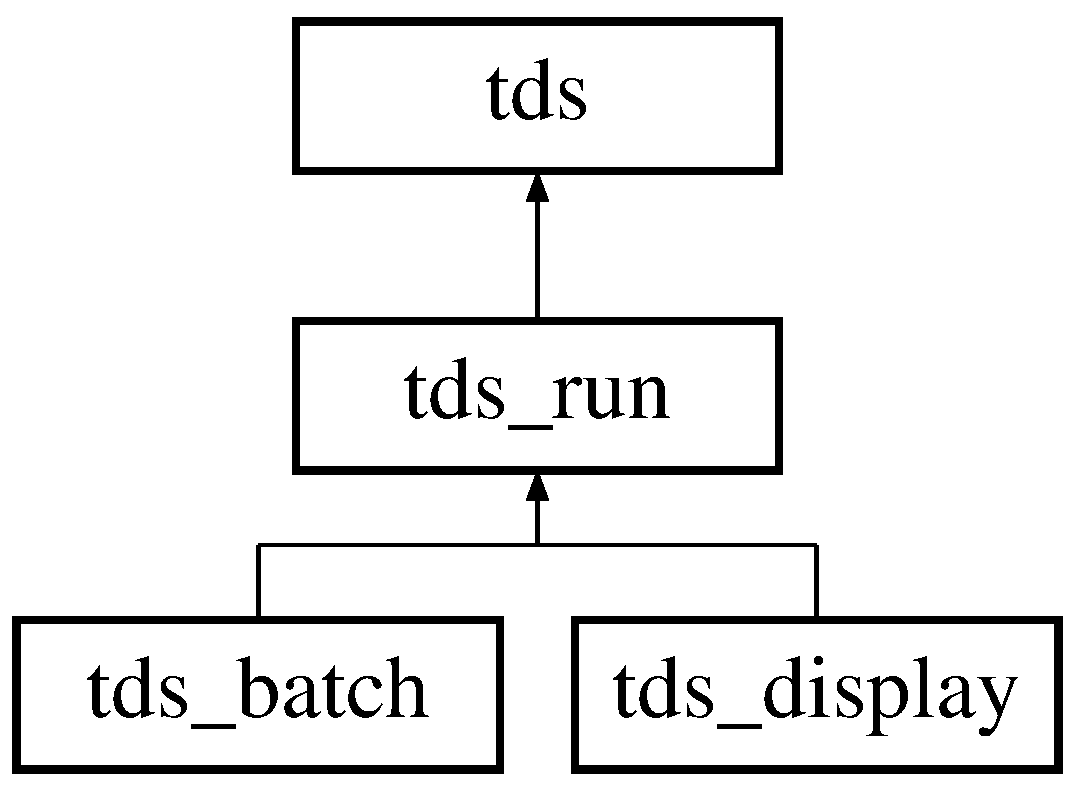
\includegraphics[height=3.000000cm]{classtds__run}
\end{center}
\end{figure}
\subsection*{Public Member Functions}
\begin{DoxyCompactItemize}
\item 
\hyperlink{classtds__run_a0ba74f360c64a7e2f3f8959dc1fed2df}{tds\+\_\+run} ()
\item 
virtual \hyperlink{classtds__run_aa2b9a0552e50ff324d03c3d420fff38c}{$\sim$tds\+\_\+run} ()
\item 
void \hyperlink{classtds__run_a9abb2736c161cf2156e3e163a04a0cd4}{check\+\_\+coincidence} ()
\item 
void \hyperlink{classtds__run_a35a3ff44173673f3128e3ef53f2ed88d}{make\+\_\+analysis} ()
\item 
void \hyperlink{classtds__run_abd30ce52c369e4df8604e572d6927284}{set\+\_\+units\+\_\+from\+\_\+file} (const char $\ast$units\+\_\+file\+\_\+address\+\_\+)
\item 
void \hyperlink{classtds__run_ae1603d896969d71fa6547abe35223f61}{initialise} ()
\item 
void \hyperlink{classtds__run_ad032df448d1a63322c2bf79f5a0096b2}{read\+\_\+run\+\_\+file} (std\+::string run\+\_\+file\+\_\+name)
\item 
void \hyperlink{classtds__run_adff2cb3deec1b483622a7dda413dda31}{process\+\_\+plugins} ()
\item 
void \hyperlink{classtds__run_a362d316bd24de6cbf82d5d3da5d4f2c0}{add\+\_\+material\+\_\+interrupt} (\hyperlink{classIPlugin}{I\+Plugin} $\ast$\+\_\+interrupter)
\item 
void \hyperlink{classtds__run_a3839266313d0fc9e3413c28dda530482}{add\+\_\+section\+\_\+interrupt} (\hyperlink{classIPlugin}{I\+Plugin} $\ast$\+\_\+interrupter)
\item 
void \hyperlink{classtds__run_ab6675a0bebfd5bed698acd4dea878d41}{add\+\_\+node\+\_\+interrupt} (\hyperlink{classIPlugin}{I\+Plugin} $\ast$\+\_\+interrupter)
\item 
void \hyperlink{classtds__run_a312b07f0d3efffd1642dfa87895ff4cc}{add\+\_\+element\+\_\+interrupt} (\hyperlink{classIPlugin}{I\+Plugin} $\ast$\+\_\+interrupter)
\item 
void \hyperlink{classtds__run_ac40a3ad881c24c25897bd1b09d78a078}{add\+\_\+element\+\_\+link\+\_\+interrupt} (\hyperlink{classIPlugin}{I\+Plugin} $\ast$\+\_\+interrupter)
\item 
void \hyperlink{classtds__run_ab4ec00a4d9f22819365b66477c10ae91}{add\+\_\+pre\+\_\+simulation\+\_\+interrupt} (\hyperlink{classIPlugin}{I\+Plugin} $\ast$\+\_\+interrupter)
\item 
void \hyperlink{classtds__run_a53af820867a6889a0f992747b025e960}{add\+\_\+start\+\_\+step\+\_\+interrupt} (\hyperlink{classIPlugin}{I\+Plugin} $\ast$\+\_\+interrupter)
\item 
void \hyperlink{classtds__run_ac0c00ed2b05ebefed18ffd4d1df9d939}{add\+\_\+end\+\_\+step\+\_\+interrupt} (\hyperlink{classIPlugin}{I\+Plugin} $\ast$\+\_\+interrupter)
\item 
void \hyperlink{classtds__run_ab00abee313469532a8ab080aca7bd646}{add\+\_\+post\+\_\+simulation\+\_\+interrupt} (\hyperlink{classIPlugin}{I\+Plugin} $\ast$\+\_\+interrupter)
\item 
void \hyperlink{classtds__run_a9374772ea6de814d7dfded259832f6b6}{change\+\_\+section\+\_\+pointer} (int \+\_\+i, \hyperlink{classtds__section}{tds\+\_\+section} $\ast$\+\_\+new\+\_\+section)
\item 
void \hyperlink{classtds__run_a03691796a9eebdfbf5bc65e5b705254c}{change\+\_\+material\+\_\+pointer} (int \+\_\+i, \hyperlink{classtds__material}{tds\+\_\+material} $\ast$\+\_\+new\+\_\+material)
\item 
void \hyperlink{classtds__run_a682cac3d47e4b6ed3e005d37041db08b}{change\+\_\+node\+\_\+pointer} (int \+\_\+i, \hyperlink{classtds__node}{tds\+\_\+node} $\ast$\+\_\+new\+\_\+node)
\item 
void \hyperlink{classtds__run_adfce89e41fb6ffe66fbbcb3dadcf101a}{change\+\_\+element\+\_\+pointer} (int \+\_\+i, \hyperlink{classtds__element}{tds\+\_\+element} $\ast$\+\_\+new\+\_\+element)
\item 
void \hyperlink{classtds__run_a43fa7246bfeda6b5e30e7064c798ce44}{basename} (std\+::string \+\_\+basename)
\item 
void \hyperlink{classtds__run_af835c5821513196c95ea1aa8843b7c4d}{configname} (std\+::string \+\_\+configname)
\item 
void \hyperlink{classtds__run_ab915e669b626f046e452bc8986dc2745}{outputname} (std\+::string \+\_\+outputname)
\item 
void \hyperlink{classtds__run_a3c6f314b5abe50031704b3993624ac98}{delta\+\_\+t} (double \+\_\+delta\+\_\+t)
\item 
void \hyperlink{classtds__run_a3ef12a27264daabbce95d66a05a1783f}{steps} (int \+\_\+steps)
\item 
void \hyperlink{classtds__run_af6c0667d9868be944a1d3e5880609f8a}{tracking\+\_\+interval} (double \+\_\+tracking\+\_\+interval)
\item 
void \hyperlink{classtds__run_a555ffb37cdd6f1a9b877ae4b3be32acb}{tracked\+\_\+elements} (std\+::vector$<$ int $>$ \&\+\_\+tracked\+\_\+elements)
\item 
void \hyperlink{classtds__run_a992893887cdbc12a5169ddb4433ed2fc}{tracked\+\_\+element} (int i, int \hyperlink{classtds_aec8ca7ac2f04016feeac7bb3f06da314}{element})
\item 
std\+::string \hyperlink{classtds__run_a137f612e6b407e454bccad95afbb21a9}{basename} ()
\item 
std\+::string \hyperlink{classtds__run_a9e8f81d142ee0b76bfd6e9e28d2b63f3}{configname} ()
\item 
std\+::string \hyperlink{classtds__run_a1d9a5d498afe05b982a0a7f748eb8210}{outputname} ()
\item 
double \hyperlink{classtds__run_a5e48a031180b7523e53378f5174d79a3}{delta\+\_\+t} ()
\item 
int \hyperlink{classtds__run_a62c2082354b12fb78a2888ab719c1ad9}{steps} ()
\item 
double \hyperlink{classtds__run_a55ac0838be1171fc81aa8c029c582074}{tracking\+\_\+interval} ()
\item 
int \hyperlink{classtds__run_a163561d49e453bae8832cea7330f2e6f}{tracked\+\_\+element} (int i)
\item 
std\+::vector$<$ int $>$ $\ast$ \hyperlink{classtds__run_aba189393afcc21e3320bef781ddbe67d}{tracked\+\_\+elements} ()
\item 
const char $\ast$ \hyperlink{classtds__run_a4d3f91ec85fde67fca2be01c65c9e055}{units\+\_\+file\+\_\+address} ()
\item 
const char $\ast$ \hyperlink{classtds__run_af89342b9231d4b99a83ff55d1ca5b969}{materials\+\_\+file\+\_\+address} ()
\item 
std\+::string \hyperlink{classtds__run_af40ce5e25f42be9e10b5477c0608f165}{sections\+\_\+file\+\_\+address} ()
\item 
std\+::string \hyperlink{classtds__run_abbf40891531e0cf9fd4c7900332fe36e}{nodes\+\_\+file\+\_\+address} ()
\item 
std\+::string \hyperlink{classtds__run_a89253a539c775d4b68c539b428127d36}{elements\+\_\+file\+\_\+address} ()
\item 
std\+::string \hyperlink{classtds__run_a8ff6cd6b421f73c0d77add4dd27e204e}{contaminations\+\_\+file\+\_\+address} ()
\item 
std\+::string \hyperlink{classtds__run_a5e46adee5b685171212fb294c282c27d}{tracking\+\_\+file\+\_\+address} ()
\end{DoxyCompactItemize}
\subsection*{Additional Inherited Members}


\subsection{Constructor \& Destructor Documentation}
\index{tds\+\_\+run@{tds\+\_\+run}!tds\+\_\+run@{tds\+\_\+run}}
\index{tds\+\_\+run@{tds\+\_\+run}!tds\+\_\+run@{tds\+\_\+run}}
\subsubsection[{\texorpdfstring{tds\+\_\+run()}{tds_run()}}]{\setlength{\rightskip}{0pt plus 5cm}tds\+\_\+run\+::tds\+\_\+run (
\begin{DoxyParamCaption}
{}
\end{DoxyParamCaption}
)}\hypertarget{classtds__run_a0ba74f360c64a7e2f3f8959dc1fed2df}{}\label{classtds__run_a0ba74f360c64a7e2f3f8959dc1fed2df}
\index{tds\+\_\+run@{tds\+\_\+run}!````~tds\+\_\+run@{$\sim$tds\+\_\+run}}
\index{````~tds\+\_\+run@{$\sim$tds\+\_\+run}!tds\+\_\+run@{tds\+\_\+run}}
\subsubsection[{\texorpdfstring{$\sim$tds\+\_\+run()}{~tds_run()}}]{\setlength{\rightskip}{0pt plus 5cm}tds\+\_\+run\+::$\sim$tds\+\_\+run (
\begin{DoxyParamCaption}
{}
\end{DoxyParamCaption}
)\hspace{0.3cm}{\ttfamily [virtual]}}\hypertarget{classtds__run_aa2b9a0552e50ff324d03c3d420fff38c}{}\label{classtds__run_aa2b9a0552e50ff324d03c3d420fff38c}


\subsection{Member Function Documentation}
\index{tds\+\_\+run@{tds\+\_\+run}!add\+\_\+element\+\_\+interrupt@{add\+\_\+element\+\_\+interrupt}}
\index{add\+\_\+element\+\_\+interrupt@{add\+\_\+element\+\_\+interrupt}!tds\+\_\+run@{tds\+\_\+run}}
\subsubsection[{\texorpdfstring{add\+\_\+element\+\_\+interrupt(\+I\+Plugin $\ast$\+\_\+interrupter)}{add_element_interrupt(IPlugin *_interrupter)}}]{\setlength{\rightskip}{0pt plus 5cm}void tds\+\_\+run\+::add\+\_\+element\+\_\+interrupt (
\begin{DoxyParamCaption}
\item[{{\bf I\+Plugin} $\ast$}]{\+\_\+interrupter}
\end{DoxyParamCaption}
)}\hypertarget{classtds__run_a312b07f0d3efffd1642dfa87895ff4cc}{}\label{classtds__run_a312b07f0d3efffd1642dfa87895ff4cc}
\index{tds\+\_\+run@{tds\+\_\+run}!add\+\_\+element\+\_\+link\+\_\+interrupt@{add\+\_\+element\+\_\+link\+\_\+interrupt}}
\index{add\+\_\+element\+\_\+link\+\_\+interrupt@{add\+\_\+element\+\_\+link\+\_\+interrupt}!tds\+\_\+run@{tds\+\_\+run}}
\subsubsection[{\texorpdfstring{add\+\_\+element\+\_\+link\+\_\+interrupt(\+I\+Plugin $\ast$\+\_\+interrupter)}{add_element_link_interrupt(IPlugin *_interrupter)}}]{\setlength{\rightskip}{0pt plus 5cm}void tds\+\_\+run\+::add\+\_\+element\+\_\+link\+\_\+interrupt (
\begin{DoxyParamCaption}
\item[{{\bf I\+Plugin} $\ast$}]{\+\_\+interrupter}
\end{DoxyParamCaption}
)}\hypertarget{classtds__run_ac40a3ad881c24c25897bd1b09d78a078}{}\label{classtds__run_ac40a3ad881c24c25897bd1b09d78a078}
\index{tds\+\_\+run@{tds\+\_\+run}!add\+\_\+end\+\_\+step\+\_\+interrupt@{add\+\_\+end\+\_\+step\+\_\+interrupt}}
\index{add\+\_\+end\+\_\+step\+\_\+interrupt@{add\+\_\+end\+\_\+step\+\_\+interrupt}!tds\+\_\+run@{tds\+\_\+run}}
\subsubsection[{\texorpdfstring{add\+\_\+end\+\_\+step\+\_\+interrupt(\+I\+Plugin $\ast$\+\_\+interrupter)}{add_end_step_interrupt(IPlugin *_interrupter)}}]{\setlength{\rightskip}{0pt plus 5cm}void tds\+\_\+run\+::add\+\_\+end\+\_\+step\+\_\+interrupt (
\begin{DoxyParamCaption}
\item[{{\bf I\+Plugin} $\ast$}]{\+\_\+interrupter}
\end{DoxyParamCaption}
)}\hypertarget{classtds__run_ac0c00ed2b05ebefed18ffd4d1df9d939}{}\label{classtds__run_ac0c00ed2b05ebefed18ffd4d1df9d939}
\index{tds\+\_\+run@{tds\+\_\+run}!add\+\_\+material\+\_\+interrupt@{add\+\_\+material\+\_\+interrupt}}
\index{add\+\_\+material\+\_\+interrupt@{add\+\_\+material\+\_\+interrupt}!tds\+\_\+run@{tds\+\_\+run}}
\subsubsection[{\texorpdfstring{add\+\_\+material\+\_\+interrupt(\+I\+Plugin $\ast$\+\_\+interrupter)}{add_material_interrupt(IPlugin *_interrupter)}}]{\setlength{\rightskip}{0pt plus 5cm}void tds\+\_\+run\+::add\+\_\+material\+\_\+interrupt (
\begin{DoxyParamCaption}
\item[{{\bf I\+Plugin} $\ast$}]{\+\_\+interrupter}
\end{DoxyParamCaption}
)}\hypertarget{classtds__run_a362d316bd24de6cbf82d5d3da5d4f2c0}{}\label{classtds__run_a362d316bd24de6cbf82d5d3da5d4f2c0}
\index{tds\+\_\+run@{tds\+\_\+run}!add\+\_\+node\+\_\+interrupt@{add\+\_\+node\+\_\+interrupt}}
\index{add\+\_\+node\+\_\+interrupt@{add\+\_\+node\+\_\+interrupt}!tds\+\_\+run@{tds\+\_\+run}}
\subsubsection[{\texorpdfstring{add\+\_\+node\+\_\+interrupt(\+I\+Plugin $\ast$\+\_\+interrupter)}{add_node_interrupt(IPlugin *_interrupter)}}]{\setlength{\rightskip}{0pt plus 5cm}void tds\+\_\+run\+::add\+\_\+node\+\_\+interrupt (
\begin{DoxyParamCaption}
\item[{{\bf I\+Plugin} $\ast$}]{\+\_\+interrupter}
\end{DoxyParamCaption}
)}\hypertarget{classtds__run_ab6675a0bebfd5bed698acd4dea878d41}{}\label{classtds__run_ab6675a0bebfd5bed698acd4dea878d41}
\index{tds\+\_\+run@{tds\+\_\+run}!add\+\_\+post\+\_\+simulation\+\_\+interrupt@{add\+\_\+post\+\_\+simulation\+\_\+interrupt}}
\index{add\+\_\+post\+\_\+simulation\+\_\+interrupt@{add\+\_\+post\+\_\+simulation\+\_\+interrupt}!tds\+\_\+run@{tds\+\_\+run}}
\subsubsection[{\texorpdfstring{add\+\_\+post\+\_\+simulation\+\_\+interrupt(\+I\+Plugin $\ast$\+\_\+interrupter)}{add_post_simulation_interrupt(IPlugin *_interrupter)}}]{\setlength{\rightskip}{0pt plus 5cm}void tds\+\_\+run\+::add\+\_\+post\+\_\+simulation\+\_\+interrupt (
\begin{DoxyParamCaption}
\item[{{\bf I\+Plugin} $\ast$}]{\+\_\+interrupter}
\end{DoxyParamCaption}
)}\hypertarget{classtds__run_ab00abee313469532a8ab080aca7bd646}{}\label{classtds__run_ab00abee313469532a8ab080aca7bd646}
\index{tds\+\_\+run@{tds\+\_\+run}!add\+\_\+pre\+\_\+simulation\+\_\+interrupt@{add\+\_\+pre\+\_\+simulation\+\_\+interrupt}}
\index{add\+\_\+pre\+\_\+simulation\+\_\+interrupt@{add\+\_\+pre\+\_\+simulation\+\_\+interrupt}!tds\+\_\+run@{tds\+\_\+run}}
\subsubsection[{\texorpdfstring{add\+\_\+pre\+\_\+simulation\+\_\+interrupt(\+I\+Plugin $\ast$\+\_\+interrupter)}{add_pre_simulation_interrupt(IPlugin *_interrupter)}}]{\setlength{\rightskip}{0pt plus 5cm}void tds\+\_\+run\+::add\+\_\+pre\+\_\+simulation\+\_\+interrupt (
\begin{DoxyParamCaption}
\item[{{\bf I\+Plugin} $\ast$}]{\+\_\+interrupter}
\end{DoxyParamCaption}
)}\hypertarget{classtds__run_ab4ec00a4d9f22819365b66477c10ae91}{}\label{classtds__run_ab4ec00a4d9f22819365b66477c10ae91}
\index{tds\+\_\+run@{tds\+\_\+run}!add\+\_\+section\+\_\+interrupt@{add\+\_\+section\+\_\+interrupt}}
\index{add\+\_\+section\+\_\+interrupt@{add\+\_\+section\+\_\+interrupt}!tds\+\_\+run@{tds\+\_\+run}}
\subsubsection[{\texorpdfstring{add\+\_\+section\+\_\+interrupt(\+I\+Plugin $\ast$\+\_\+interrupter)}{add_section_interrupt(IPlugin *_interrupter)}}]{\setlength{\rightskip}{0pt plus 5cm}void tds\+\_\+run\+::add\+\_\+section\+\_\+interrupt (
\begin{DoxyParamCaption}
\item[{{\bf I\+Plugin} $\ast$}]{\+\_\+interrupter}
\end{DoxyParamCaption}
)}\hypertarget{classtds__run_a3839266313d0fc9e3413c28dda530482}{}\label{classtds__run_a3839266313d0fc9e3413c28dda530482}
\index{tds\+\_\+run@{tds\+\_\+run}!add\+\_\+start\+\_\+step\+\_\+interrupt@{add\+\_\+start\+\_\+step\+\_\+interrupt}}
\index{add\+\_\+start\+\_\+step\+\_\+interrupt@{add\+\_\+start\+\_\+step\+\_\+interrupt}!tds\+\_\+run@{tds\+\_\+run}}
\subsubsection[{\texorpdfstring{add\+\_\+start\+\_\+step\+\_\+interrupt(\+I\+Plugin $\ast$\+\_\+interrupter)}{add_start_step_interrupt(IPlugin *_interrupter)}}]{\setlength{\rightskip}{0pt plus 5cm}void tds\+\_\+run\+::add\+\_\+start\+\_\+step\+\_\+interrupt (
\begin{DoxyParamCaption}
\item[{{\bf I\+Plugin} $\ast$}]{\+\_\+interrupter}
\end{DoxyParamCaption}
)}\hypertarget{classtds__run_a53af820867a6889a0f992747b025e960}{}\label{classtds__run_a53af820867a6889a0f992747b025e960}
\index{tds\+\_\+run@{tds\+\_\+run}!basename@{basename}}
\index{basename@{basename}!tds\+\_\+run@{tds\+\_\+run}}
\subsubsection[{\texorpdfstring{basename(std\+::string \+\_\+basename)}{basename(std::string _basename)}}]{\setlength{\rightskip}{0pt plus 5cm}void tds\+\_\+run\+::basename (
\begin{DoxyParamCaption}
\item[{std\+::string}]{\+\_\+basename}
\end{DoxyParamCaption}
)\hspace{0.3cm}{\ttfamily [inline]}}\hypertarget{classtds__run_a43fa7246bfeda6b5e30e7064c798ce44}{}\label{classtds__run_a43fa7246bfeda6b5e30e7064c798ce44}
\index{tds\+\_\+run@{tds\+\_\+run}!basename@{basename}}
\index{basename@{basename}!tds\+\_\+run@{tds\+\_\+run}}
\subsubsection[{\texorpdfstring{basename()}{basename()}}]{\setlength{\rightskip}{0pt plus 5cm}std\+::string tds\+\_\+run\+::basename (
\begin{DoxyParamCaption}
{}
\end{DoxyParamCaption}
)\hspace{0.3cm}{\ttfamily [inline]}}\hypertarget{classtds__run_a137f612e6b407e454bccad95afbb21a9}{}\label{classtds__run_a137f612e6b407e454bccad95afbb21a9}
\index{tds\+\_\+run@{tds\+\_\+run}!change\+\_\+element\+\_\+pointer@{change\+\_\+element\+\_\+pointer}}
\index{change\+\_\+element\+\_\+pointer@{change\+\_\+element\+\_\+pointer}!tds\+\_\+run@{tds\+\_\+run}}
\subsubsection[{\texorpdfstring{change\+\_\+element\+\_\+pointer(int \+\_\+i, tds\+\_\+element $\ast$\+\_\+new\+\_\+element)}{change_element_pointer(int _i, tds_element *_new_element)}}]{\setlength{\rightskip}{0pt plus 5cm}void tds\+\_\+run\+::change\+\_\+element\+\_\+pointer (
\begin{DoxyParamCaption}
\item[{int}]{\+\_\+i, }
\item[{{\bf tds\+\_\+element} $\ast$}]{\+\_\+new\+\_\+element}
\end{DoxyParamCaption}
)}\hypertarget{classtds__run_adfce89e41fb6ffe66fbbcb3dadcf101a}{}\label{classtds__run_adfce89e41fb6ffe66fbbcb3dadcf101a}
\index{tds\+\_\+run@{tds\+\_\+run}!change\+\_\+material\+\_\+pointer@{change\+\_\+material\+\_\+pointer}}
\index{change\+\_\+material\+\_\+pointer@{change\+\_\+material\+\_\+pointer}!tds\+\_\+run@{tds\+\_\+run}}
\subsubsection[{\texorpdfstring{change\+\_\+material\+\_\+pointer(int \+\_\+i, tds\+\_\+material $\ast$\+\_\+new\+\_\+material)}{change_material_pointer(int _i, tds_material *_new_material)}}]{\setlength{\rightskip}{0pt plus 5cm}void tds\+\_\+run\+::change\+\_\+material\+\_\+pointer (
\begin{DoxyParamCaption}
\item[{int}]{\+\_\+i, }
\item[{{\bf tds\+\_\+material} $\ast$}]{\+\_\+new\+\_\+material}
\end{DoxyParamCaption}
)}\hypertarget{classtds__run_a03691796a9eebdfbf5bc65e5b705254c}{}\label{classtds__run_a03691796a9eebdfbf5bc65e5b705254c}
\index{tds\+\_\+run@{tds\+\_\+run}!change\+\_\+node\+\_\+pointer@{change\+\_\+node\+\_\+pointer}}
\index{change\+\_\+node\+\_\+pointer@{change\+\_\+node\+\_\+pointer}!tds\+\_\+run@{tds\+\_\+run}}
\subsubsection[{\texorpdfstring{change\+\_\+node\+\_\+pointer(int \+\_\+i, tds\+\_\+node $\ast$\+\_\+new\+\_\+node)}{change_node_pointer(int _i, tds_node *_new_node)}}]{\setlength{\rightskip}{0pt plus 5cm}void tds\+\_\+run\+::change\+\_\+node\+\_\+pointer (
\begin{DoxyParamCaption}
\item[{int}]{\+\_\+i, }
\item[{{\bf tds\+\_\+node} $\ast$}]{\+\_\+new\+\_\+node}
\end{DoxyParamCaption}
)}\hypertarget{classtds__run_a682cac3d47e4b6ed3e005d37041db08b}{}\label{classtds__run_a682cac3d47e4b6ed3e005d37041db08b}
\index{tds\+\_\+run@{tds\+\_\+run}!change\+\_\+section\+\_\+pointer@{change\+\_\+section\+\_\+pointer}}
\index{change\+\_\+section\+\_\+pointer@{change\+\_\+section\+\_\+pointer}!tds\+\_\+run@{tds\+\_\+run}}
\subsubsection[{\texorpdfstring{change\+\_\+section\+\_\+pointer(int \+\_\+i, tds\+\_\+section $\ast$\+\_\+new\+\_\+section)}{change_section_pointer(int _i, tds_section *_new_section)}}]{\setlength{\rightskip}{0pt plus 5cm}void tds\+\_\+run\+::change\+\_\+section\+\_\+pointer (
\begin{DoxyParamCaption}
\item[{int}]{\+\_\+i, }
\item[{{\bf tds\+\_\+section} $\ast$}]{\+\_\+new\+\_\+section}
\end{DoxyParamCaption}
)}\hypertarget{classtds__run_a9374772ea6de814d7dfded259832f6b6}{}\label{classtds__run_a9374772ea6de814d7dfded259832f6b6}
\index{tds\+\_\+run@{tds\+\_\+run}!check\+\_\+coincidence@{check\+\_\+coincidence}}
\index{check\+\_\+coincidence@{check\+\_\+coincidence}!tds\+\_\+run@{tds\+\_\+run}}
\subsubsection[{\texorpdfstring{check\+\_\+coincidence()}{check_coincidence()}}]{\setlength{\rightskip}{0pt plus 5cm}void tds\+\_\+run\+::check\+\_\+coincidence (
\begin{DoxyParamCaption}
{}
\end{DoxyParamCaption}
)}\hypertarget{classtds__run_a9abb2736c161cf2156e3e163a04a0cd4}{}\label{classtds__run_a9abb2736c161cf2156e3e163a04a0cd4}
\index{tds\+\_\+run@{tds\+\_\+run}!configname@{configname}}
\index{configname@{configname}!tds\+\_\+run@{tds\+\_\+run}}
\subsubsection[{\texorpdfstring{configname(std\+::string \+\_\+configname)}{configname(std::string _configname)}}]{\setlength{\rightskip}{0pt plus 5cm}void tds\+\_\+run\+::configname (
\begin{DoxyParamCaption}
\item[{std\+::string}]{\+\_\+configname}
\end{DoxyParamCaption}
)\hspace{0.3cm}{\ttfamily [inline]}}\hypertarget{classtds__run_af835c5821513196c95ea1aa8843b7c4d}{}\label{classtds__run_af835c5821513196c95ea1aa8843b7c4d}
\index{tds\+\_\+run@{tds\+\_\+run}!configname@{configname}}
\index{configname@{configname}!tds\+\_\+run@{tds\+\_\+run}}
\subsubsection[{\texorpdfstring{configname()}{configname()}}]{\setlength{\rightskip}{0pt plus 5cm}std\+::string tds\+\_\+run\+::configname (
\begin{DoxyParamCaption}
{}
\end{DoxyParamCaption}
)\hspace{0.3cm}{\ttfamily [inline]}}\hypertarget{classtds__run_a9e8f81d142ee0b76bfd6e9e28d2b63f3}{}\label{classtds__run_a9e8f81d142ee0b76bfd6e9e28d2b63f3}
\index{tds\+\_\+run@{tds\+\_\+run}!contaminations\+\_\+file\+\_\+address@{contaminations\+\_\+file\+\_\+address}}
\index{contaminations\+\_\+file\+\_\+address@{contaminations\+\_\+file\+\_\+address}!tds\+\_\+run@{tds\+\_\+run}}
\subsubsection[{\texorpdfstring{contaminations\+\_\+file\+\_\+address()}{contaminations_file_address()}}]{\setlength{\rightskip}{0pt plus 5cm}std\+::string tds\+\_\+run\+::contaminations\+\_\+file\+\_\+address (
\begin{DoxyParamCaption}
{}
\end{DoxyParamCaption}
)\hspace{0.3cm}{\ttfamily [inline]}}\hypertarget{classtds__run_a8ff6cd6b421f73c0d77add4dd27e204e}{}\label{classtds__run_a8ff6cd6b421f73c0d77add4dd27e204e}
\index{tds\+\_\+run@{tds\+\_\+run}!delta\+\_\+t@{delta\+\_\+t}}
\index{delta\+\_\+t@{delta\+\_\+t}!tds\+\_\+run@{tds\+\_\+run}}
\subsubsection[{\texorpdfstring{delta\+\_\+t(double \+\_\+delta\+\_\+t)}{delta_t(double _delta_t)}}]{\setlength{\rightskip}{0pt plus 5cm}void tds\+\_\+run\+::delta\+\_\+t (
\begin{DoxyParamCaption}
\item[{double}]{\+\_\+delta\+\_\+t}
\end{DoxyParamCaption}
)\hspace{0.3cm}{\ttfamily [inline]}}\hypertarget{classtds__run_a3c6f314b5abe50031704b3993624ac98}{}\label{classtds__run_a3c6f314b5abe50031704b3993624ac98}
\index{tds\+\_\+run@{tds\+\_\+run}!delta\+\_\+t@{delta\+\_\+t}}
\index{delta\+\_\+t@{delta\+\_\+t}!tds\+\_\+run@{tds\+\_\+run}}
\subsubsection[{\texorpdfstring{delta\+\_\+t()}{delta_t()}}]{\setlength{\rightskip}{0pt plus 5cm}double tds\+\_\+run\+::delta\+\_\+t (
\begin{DoxyParamCaption}
{}
\end{DoxyParamCaption}
)\hspace{0.3cm}{\ttfamily [inline]}}\hypertarget{classtds__run_a5e48a031180b7523e53378f5174d79a3}{}\label{classtds__run_a5e48a031180b7523e53378f5174d79a3}
\index{tds\+\_\+run@{tds\+\_\+run}!elements\+\_\+file\+\_\+address@{elements\+\_\+file\+\_\+address}}
\index{elements\+\_\+file\+\_\+address@{elements\+\_\+file\+\_\+address}!tds\+\_\+run@{tds\+\_\+run}}
\subsubsection[{\texorpdfstring{elements\+\_\+file\+\_\+address()}{elements_file_address()}}]{\setlength{\rightskip}{0pt plus 5cm}std\+::string tds\+\_\+run\+::elements\+\_\+file\+\_\+address (
\begin{DoxyParamCaption}
{}
\end{DoxyParamCaption}
)\hspace{0.3cm}{\ttfamily [inline]}}\hypertarget{classtds__run_a89253a539c775d4b68c539b428127d36}{}\label{classtds__run_a89253a539c775d4b68c539b428127d36}
\index{tds\+\_\+run@{tds\+\_\+run}!initialise@{initialise}}
\index{initialise@{initialise}!tds\+\_\+run@{tds\+\_\+run}}
\subsubsection[{\texorpdfstring{initialise()}{initialise()}}]{\setlength{\rightskip}{0pt plus 5cm}void tds\+\_\+run\+::initialise (
\begin{DoxyParamCaption}
{}
\end{DoxyParamCaption}
)}\hypertarget{classtds__run_ae1603d896969d71fa6547abe35223f61}{}\label{classtds__run_ae1603d896969d71fa6547abe35223f61}
\index{tds\+\_\+run@{tds\+\_\+run}!make\+\_\+analysis@{make\+\_\+analysis}}
\index{make\+\_\+analysis@{make\+\_\+analysis}!tds\+\_\+run@{tds\+\_\+run}}
\subsubsection[{\texorpdfstring{make\+\_\+analysis()}{make_analysis()}}]{\setlength{\rightskip}{0pt plus 5cm}void tds\+\_\+run\+::make\+\_\+analysis (
\begin{DoxyParamCaption}
{}
\end{DoxyParamCaption}
)}\hypertarget{classtds__run_a35a3ff44173673f3128e3ef53f2ed88d}{}\label{classtds__run_a35a3ff44173673f3128e3ef53f2ed88d}
\index{tds\+\_\+run@{tds\+\_\+run}!materials\+\_\+file\+\_\+address@{materials\+\_\+file\+\_\+address}}
\index{materials\+\_\+file\+\_\+address@{materials\+\_\+file\+\_\+address}!tds\+\_\+run@{tds\+\_\+run}}
\subsubsection[{\texorpdfstring{materials\+\_\+file\+\_\+address()}{materials_file_address()}}]{\setlength{\rightskip}{0pt plus 5cm}const char$\ast$ tds\+\_\+run\+::materials\+\_\+file\+\_\+address (
\begin{DoxyParamCaption}
{}
\end{DoxyParamCaption}
)\hspace{0.3cm}{\ttfamily [inline]}}\hypertarget{classtds__run_af89342b9231d4b99a83ff55d1ca5b969}{}\label{classtds__run_af89342b9231d4b99a83ff55d1ca5b969}
\index{tds\+\_\+run@{tds\+\_\+run}!nodes\+\_\+file\+\_\+address@{nodes\+\_\+file\+\_\+address}}
\index{nodes\+\_\+file\+\_\+address@{nodes\+\_\+file\+\_\+address}!tds\+\_\+run@{tds\+\_\+run}}
\subsubsection[{\texorpdfstring{nodes\+\_\+file\+\_\+address()}{nodes_file_address()}}]{\setlength{\rightskip}{0pt plus 5cm}std\+::string tds\+\_\+run\+::nodes\+\_\+file\+\_\+address (
\begin{DoxyParamCaption}
{}
\end{DoxyParamCaption}
)\hspace{0.3cm}{\ttfamily [inline]}}\hypertarget{classtds__run_abbf40891531e0cf9fd4c7900332fe36e}{}\label{classtds__run_abbf40891531e0cf9fd4c7900332fe36e}
\index{tds\+\_\+run@{tds\+\_\+run}!outputname@{outputname}}
\index{outputname@{outputname}!tds\+\_\+run@{tds\+\_\+run}}
\subsubsection[{\texorpdfstring{outputname(std\+::string \+\_\+outputname)}{outputname(std::string _outputname)}}]{\setlength{\rightskip}{0pt plus 5cm}void tds\+\_\+run\+::outputname (
\begin{DoxyParamCaption}
\item[{std\+::string}]{\+\_\+outputname}
\end{DoxyParamCaption}
)\hspace{0.3cm}{\ttfamily [inline]}}\hypertarget{classtds__run_ab915e669b626f046e452bc8986dc2745}{}\label{classtds__run_ab915e669b626f046e452bc8986dc2745}
\index{tds\+\_\+run@{tds\+\_\+run}!outputname@{outputname}}
\index{outputname@{outputname}!tds\+\_\+run@{tds\+\_\+run}}
\subsubsection[{\texorpdfstring{outputname()}{outputname()}}]{\setlength{\rightskip}{0pt plus 5cm}std\+::string tds\+\_\+run\+::outputname (
\begin{DoxyParamCaption}
{}
\end{DoxyParamCaption}
)\hspace{0.3cm}{\ttfamily [inline]}}\hypertarget{classtds__run_a1d9a5d498afe05b982a0a7f748eb8210}{}\label{classtds__run_a1d9a5d498afe05b982a0a7f748eb8210}
\index{tds\+\_\+run@{tds\+\_\+run}!process\+\_\+plugins@{process\+\_\+plugins}}
\index{process\+\_\+plugins@{process\+\_\+plugins}!tds\+\_\+run@{tds\+\_\+run}}
\subsubsection[{\texorpdfstring{process\+\_\+plugins()}{process_plugins()}}]{\setlength{\rightskip}{0pt plus 5cm}void tds\+\_\+run\+::process\+\_\+plugins (
\begin{DoxyParamCaption}
{}
\end{DoxyParamCaption}
)}\hypertarget{classtds__run_adff2cb3deec1b483622a7dda413dda31}{}\label{classtds__run_adff2cb3deec1b483622a7dda413dda31}
\index{tds\+\_\+run@{tds\+\_\+run}!read\+\_\+run\+\_\+file@{read\+\_\+run\+\_\+file}}
\index{read\+\_\+run\+\_\+file@{read\+\_\+run\+\_\+file}!tds\+\_\+run@{tds\+\_\+run}}
\subsubsection[{\texorpdfstring{read\+\_\+run\+\_\+file(std\+::string run\+\_\+file\+\_\+name)}{read_run_file(std::string run_file_name)}}]{\setlength{\rightskip}{0pt plus 5cm}void tds\+\_\+run\+::read\+\_\+run\+\_\+file (
\begin{DoxyParamCaption}
\item[{std\+::string}]{run\+\_\+file\+\_\+name}
\end{DoxyParamCaption}
)}\hypertarget{classtds__run_ad032df448d1a63322c2bf79f5a0096b2}{}\label{classtds__run_ad032df448d1a63322c2bf79f5a0096b2}
\index{tds\+\_\+run@{tds\+\_\+run}!sections\+\_\+file\+\_\+address@{sections\+\_\+file\+\_\+address}}
\index{sections\+\_\+file\+\_\+address@{sections\+\_\+file\+\_\+address}!tds\+\_\+run@{tds\+\_\+run}}
\subsubsection[{\texorpdfstring{sections\+\_\+file\+\_\+address()}{sections_file_address()}}]{\setlength{\rightskip}{0pt plus 5cm}std\+::string tds\+\_\+run\+::sections\+\_\+file\+\_\+address (
\begin{DoxyParamCaption}
{}
\end{DoxyParamCaption}
)\hspace{0.3cm}{\ttfamily [inline]}}\hypertarget{classtds__run_af40ce5e25f42be9e10b5477c0608f165}{}\label{classtds__run_af40ce5e25f42be9e10b5477c0608f165}
\index{tds\+\_\+run@{tds\+\_\+run}!set\+\_\+units\+\_\+from\+\_\+file@{set\+\_\+units\+\_\+from\+\_\+file}}
\index{set\+\_\+units\+\_\+from\+\_\+file@{set\+\_\+units\+\_\+from\+\_\+file}!tds\+\_\+run@{tds\+\_\+run}}
\subsubsection[{\texorpdfstring{set\+\_\+units\+\_\+from\+\_\+file(const char $\ast$units\+\_\+file\+\_\+address\+\_\+)}{set_units_from_file(const char *units_file_address_)}}]{\setlength{\rightskip}{0pt plus 5cm}void tds\+\_\+run\+::set\+\_\+units\+\_\+from\+\_\+file (
\begin{DoxyParamCaption}
\item[{const char $\ast$}]{units\+\_\+file\+\_\+address\+\_\+}
\end{DoxyParamCaption}
)}\hypertarget{classtds__run_abd30ce52c369e4df8604e572d6927284}{}\label{classtds__run_abd30ce52c369e4df8604e572d6927284}
\index{tds\+\_\+run@{tds\+\_\+run}!steps@{steps}}
\index{steps@{steps}!tds\+\_\+run@{tds\+\_\+run}}
\subsubsection[{\texorpdfstring{steps(int \+\_\+steps)}{steps(int _steps)}}]{\setlength{\rightskip}{0pt plus 5cm}void tds\+\_\+run\+::steps (
\begin{DoxyParamCaption}
\item[{int}]{\+\_\+steps}
\end{DoxyParamCaption}
)\hspace{0.3cm}{\ttfamily [inline]}}\hypertarget{classtds__run_a3ef12a27264daabbce95d66a05a1783f}{}\label{classtds__run_a3ef12a27264daabbce95d66a05a1783f}
\index{tds\+\_\+run@{tds\+\_\+run}!steps@{steps}}
\index{steps@{steps}!tds\+\_\+run@{tds\+\_\+run}}
\subsubsection[{\texorpdfstring{steps()}{steps()}}]{\setlength{\rightskip}{0pt plus 5cm}int tds\+\_\+run\+::steps (
\begin{DoxyParamCaption}
{}
\end{DoxyParamCaption}
)\hspace{0.3cm}{\ttfamily [inline]}}\hypertarget{classtds__run_a62c2082354b12fb78a2888ab719c1ad9}{}\label{classtds__run_a62c2082354b12fb78a2888ab719c1ad9}
\index{tds\+\_\+run@{tds\+\_\+run}!tracked\+\_\+element@{tracked\+\_\+element}}
\index{tracked\+\_\+element@{tracked\+\_\+element}!tds\+\_\+run@{tds\+\_\+run}}
\subsubsection[{\texorpdfstring{tracked\+\_\+element(int i, int element)}{tracked_element(int i, int element)}}]{\setlength{\rightskip}{0pt plus 5cm}void tds\+\_\+run\+::tracked\+\_\+element (
\begin{DoxyParamCaption}
\item[{int}]{i, }
\item[{int}]{element}
\end{DoxyParamCaption}
)\hspace{0.3cm}{\ttfamily [inline]}}\hypertarget{classtds__run_a992893887cdbc12a5169ddb4433ed2fc}{}\label{classtds__run_a992893887cdbc12a5169ddb4433ed2fc}
\index{tds\+\_\+run@{tds\+\_\+run}!tracked\+\_\+element@{tracked\+\_\+element}}
\index{tracked\+\_\+element@{tracked\+\_\+element}!tds\+\_\+run@{tds\+\_\+run}}
\subsubsection[{\texorpdfstring{tracked\+\_\+element(int i)}{tracked_element(int i)}}]{\setlength{\rightskip}{0pt plus 5cm}int tds\+\_\+run\+::tracked\+\_\+element (
\begin{DoxyParamCaption}
\item[{int}]{i}
\end{DoxyParamCaption}
)\hspace{0.3cm}{\ttfamily [inline]}}\hypertarget{classtds__run_a163561d49e453bae8832cea7330f2e6f}{}\label{classtds__run_a163561d49e453bae8832cea7330f2e6f}
\index{tds\+\_\+run@{tds\+\_\+run}!tracked\+\_\+elements@{tracked\+\_\+elements}}
\index{tracked\+\_\+elements@{tracked\+\_\+elements}!tds\+\_\+run@{tds\+\_\+run}}
\subsubsection[{\texorpdfstring{tracked\+\_\+elements(std\+::vector$<$ int $>$ \&\+\_\+tracked\+\_\+elements)}{tracked_elements(std::vector< int > &_tracked_elements)}}]{\setlength{\rightskip}{0pt plus 5cm}void tds\+\_\+run\+::tracked\+\_\+elements (
\begin{DoxyParamCaption}
\item[{std\+::vector$<$ int $>$ \&}]{\+\_\+tracked\+\_\+elements}
\end{DoxyParamCaption}
)\hspace{0.3cm}{\ttfamily [inline]}}\hypertarget{classtds__run_a555ffb37cdd6f1a9b877ae4b3be32acb}{}\label{classtds__run_a555ffb37cdd6f1a9b877ae4b3be32acb}
\index{tds\+\_\+run@{tds\+\_\+run}!tracked\+\_\+elements@{tracked\+\_\+elements}}
\index{tracked\+\_\+elements@{tracked\+\_\+elements}!tds\+\_\+run@{tds\+\_\+run}}
\subsubsection[{\texorpdfstring{tracked\+\_\+elements()}{tracked_elements()}}]{\setlength{\rightskip}{0pt plus 5cm}std\+::vector$<$int$>$$\ast$ tds\+\_\+run\+::tracked\+\_\+elements (
\begin{DoxyParamCaption}
{}
\end{DoxyParamCaption}
)\hspace{0.3cm}{\ttfamily [inline]}}\hypertarget{classtds__run_aba189393afcc21e3320bef781ddbe67d}{}\label{classtds__run_aba189393afcc21e3320bef781ddbe67d}
\index{tds\+\_\+run@{tds\+\_\+run}!tracking\+\_\+file\+\_\+address@{tracking\+\_\+file\+\_\+address}}
\index{tracking\+\_\+file\+\_\+address@{tracking\+\_\+file\+\_\+address}!tds\+\_\+run@{tds\+\_\+run}}
\subsubsection[{\texorpdfstring{tracking\+\_\+file\+\_\+address()}{tracking_file_address()}}]{\setlength{\rightskip}{0pt plus 5cm}std\+::string tds\+\_\+run\+::tracking\+\_\+file\+\_\+address (
\begin{DoxyParamCaption}
{}
\end{DoxyParamCaption}
)\hspace{0.3cm}{\ttfamily [inline]}}\hypertarget{classtds__run_a5e46adee5b685171212fb294c282c27d}{}\label{classtds__run_a5e46adee5b685171212fb294c282c27d}
\index{tds\+\_\+run@{tds\+\_\+run}!tracking\+\_\+interval@{tracking\+\_\+interval}}
\index{tracking\+\_\+interval@{tracking\+\_\+interval}!tds\+\_\+run@{tds\+\_\+run}}
\subsubsection[{\texorpdfstring{tracking\+\_\+interval(double \+\_\+tracking\+\_\+interval)}{tracking_interval(double _tracking_interval)}}]{\setlength{\rightskip}{0pt plus 5cm}void tds\+\_\+run\+::tracking\+\_\+interval (
\begin{DoxyParamCaption}
\item[{double}]{\+\_\+tracking\+\_\+interval}
\end{DoxyParamCaption}
)\hspace{0.3cm}{\ttfamily [inline]}}\hypertarget{classtds__run_af6c0667d9868be944a1d3e5880609f8a}{}\label{classtds__run_af6c0667d9868be944a1d3e5880609f8a}
\index{tds\+\_\+run@{tds\+\_\+run}!tracking\+\_\+interval@{tracking\+\_\+interval}}
\index{tracking\+\_\+interval@{tracking\+\_\+interval}!tds\+\_\+run@{tds\+\_\+run}}
\subsubsection[{\texorpdfstring{tracking\+\_\+interval()}{tracking_interval()}}]{\setlength{\rightskip}{0pt plus 5cm}double tds\+\_\+run\+::tracking\+\_\+interval (
\begin{DoxyParamCaption}
{}
\end{DoxyParamCaption}
)\hspace{0.3cm}{\ttfamily [inline]}}\hypertarget{classtds__run_a55ac0838be1171fc81aa8c029c582074}{}\label{classtds__run_a55ac0838be1171fc81aa8c029c582074}
\index{tds\+\_\+run@{tds\+\_\+run}!units\+\_\+file\+\_\+address@{units\+\_\+file\+\_\+address}}
\index{units\+\_\+file\+\_\+address@{units\+\_\+file\+\_\+address}!tds\+\_\+run@{tds\+\_\+run}}
\subsubsection[{\texorpdfstring{units\+\_\+file\+\_\+address()}{units_file_address()}}]{\setlength{\rightskip}{0pt plus 5cm}const char$\ast$ tds\+\_\+run\+::units\+\_\+file\+\_\+address (
\begin{DoxyParamCaption}
{}
\end{DoxyParamCaption}
)\hspace{0.3cm}{\ttfamily [inline]}}\hypertarget{classtds__run_a4d3f91ec85fde67fca2be01c65c9e055}{}\label{classtds__run_a4d3f91ec85fde67fca2be01c65c9e055}


The documentation for this class was generated from the following files\+:\begin{DoxyCompactItemize}
\item 
\hyperlink{tds_8hh}{tds.\+hh}\item 
\hyperlink{tds_8cc}{tds.\+cc}\end{DoxyCompactItemize}

\hypertarget{classtds__section}{\section{tds\-\_\-section Class Reference}
\label{classtds__section}\index{tds\-\_\-section@{tds\-\_\-section}}
}


{\ttfamily \#include $<$tds\-\_\-parts.\-hh$>$}

\subsection*{Public Member Functions}
\begin{DoxyCompactItemize}
\item 
\hyperlink{classtds__section_ab65969b3d4b2950a5f3d2178c92c6554}{tds\-\_\-section} (std\-::string \-\_\-name, \hyperlink{classtds__material}{tds\-\_\-material} $\ast$\-\_\-material)
\item 
virtual \hyperlink{classtds__section_aa81d43b2bda7a4bff6f21003f9dd6c62}{$\sim$tds\-\_\-section} ()
\item 
int \hyperlink{classtds__section_ac7f7a6748643e80fe3380c342e146cd7}{add\-\_\-element} (\hyperlink{classtds__element}{tds\-\_\-element} $\ast$new\-\_\-element)
\item 
void \hyperlink{classtds__section_ae177ecffb63403be5318c081340b0215}{clean\-\_\-elements} ()
\item 
void \hyperlink{classtds__section_ab5ed7bcffdcf61ac015a82c02cda876e}{name} (std\-::string \-\_\-name)
\item 
void \hyperlink{classtds__section_a6da38cfd02f9ef8f8d04fc71da2623fd}{material} (\hyperlink{classtds__material}{tds\-\_\-material} $\ast$\-\_\-material)
\item 
std\-::string \hyperlink{classtds__section_aee79d0125477377b79482b60fbc20fd5}{name} ()
\item 
\hyperlink{classtds__material}{tds\-\_\-material} \& \hyperlink{classtds__section_a0cfa87f9a83bc0535bb08bdbc5c8700c}{material} ()
\item 
\hyperlink{classtds__element}{tds\-\_\-element} \& \hyperlink{classtds__section_acd171d99c4648513baadcbfd994ea301}{element} (int i)
\item 
void \hyperlink{classtds__section_a429ae2483cc8952120b2a9d828aab405}{element} (int i, \hyperlink{classtds__element}{tds\-\_\-element} $\ast$\-\_\-new\-\_\-element)
\item 
int \hyperlink{classtds__section_a8aa5f42733f88e55f360f98aeb343890}{n\-\_\-elements} ()
\end{DoxyCompactItemize}


\subsection{Constructor \& Destructor Documentation}
\hypertarget{classtds__section_ab65969b3d4b2950a5f3d2178c92c6554}{\index{tds\-\_\-section@{tds\-\_\-section}!tds\-\_\-section@{tds\-\_\-section}}
\index{tds\-\_\-section@{tds\-\_\-section}!tds_section@{tds\-\_\-section}}
\subsubsection[{tds\-\_\-section}]{\setlength{\rightskip}{0pt plus 5cm}tds\-\_\-section\-::tds\-\_\-section (
\begin{DoxyParamCaption}
\item[{std\-::string}]{\-\_\-name, }
\item[{{\bf tds\-\_\-material} $\ast$}]{\-\_\-material}
\end{DoxyParamCaption}
)}}\label{classtds__section_ab65969b3d4b2950a5f3d2178c92c6554}
\hypertarget{classtds__section_aa81d43b2bda7a4bff6f21003f9dd6c62}{\index{tds\-\_\-section@{tds\-\_\-section}!$\sim$tds\-\_\-section@{$\sim$tds\-\_\-section}}
\index{$\sim$tds\-\_\-section@{$\sim$tds\-\_\-section}!tds_section@{tds\-\_\-section}}
\subsubsection[{$\sim$tds\-\_\-section}]{\setlength{\rightskip}{0pt plus 5cm}tds\-\_\-section\-::$\sim$tds\-\_\-section (
\begin{DoxyParamCaption}
{}
\end{DoxyParamCaption}
)\hspace{0.3cm}{\ttfamily [virtual]}}}\label{classtds__section_aa81d43b2bda7a4bff6f21003f9dd6c62}


\subsection{Member Function Documentation}
\hypertarget{classtds__section_ac7f7a6748643e80fe3380c342e146cd7}{\index{tds\-\_\-section@{tds\-\_\-section}!add\-\_\-element@{add\-\_\-element}}
\index{add\-\_\-element@{add\-\_\-element}!tds_section@{tds\-\_\-section}}
\subsubsection[{add\-\_\-element}]{\setlength{\rightskip}{0pt plus 5cm}int tds\-\_\-section\-::add\-\_\-element (
\begin{DoxyParamCaption}
\item[{{\bf tds\-\_\-element} $\ast$}]{new\-\_\-element}
\end{DoxyParamCaption}
)}}\label{classtds__section_ac7f7a6748643e80fe3380c342e146cd7}
\hypertarget{classtds__section_ae177ecffb63403be5318c081340b0215}{\index{tds\-\_\-section@{tds\-\_\-section}!clean\-\_\-elements@{clean\-\_\-elements}}
\index{clean\-\_\-elements@{clean\-\_\-elements}!tds_section@{tds\-\_\-section}}
\subsubsection[{clean\-\_\-elements}]{\setlength{\rightskip}{0pt plus 5cm}void tds\-\_\-section\-::clean\-\_\-elements (
\begin{DoxyParamCaption}
{}
\end{DoxyParamCaption}
)}}\label{classtds__section_ae177ecffb63403be5318c081340b0215}
\hypertarget{classtds__section_acd171d99c4648513baadcbfd994ea301}{\index{tds\-\_\-section@{tds\-\_\-section}!element@{element}}
\index{element@{element}!tds_section@{tds\-\_\-section}}
\subsubsection[{element}]{\setlength{\rightskip}{0pt plus 5cm}{\bf tds\-\_\-element}\& tds\-\_\-section\-::element (
\begin{DoxyParamCaption}
\item[{int}]{i}
\end{DoxyParamCaption}
)\hspace{0.3cm}{\ttfamily [inline]}}}\label{classtds__section_acd171d99c4648513baadcbfd994ea301}
\hypertarget{classtds__section_a429ae2483cc8952120b2a9d828aab405}{\index{tds\-\_\-section@{tds\-\_\-section}!element@{element}}
\index{element@{element}!tds_section@{tds\-\_\-section}}
\subsubsection[{element}]{\setlength{\rightskip}{0pt plus 5cm}void tds\-\_\-section\-::element (
\begin{DoxyParamCaption}
\item[{int}]{i, }
\item[{{\bf tds\-\_\-element} $\ast$}]{\-\_\-new\-\_\-element}
\end{DoxyParamCaption}
)\hspace{0.3cm}{\ttfamily [inline]}}}\label{classtds__section_a429ae2483cc8952120b2a9d828aab405}
\hypertarget{classtds__section_a6da38cfd02f9ef8f8d04fc71da2623fd}{\index{tds\-\_\-section@{tds\-\_\-section}!material@{material}}
\index{material@{material}!tds_section@{tds\-\_\-section}}
\subsubsection[{material}]{\setlength{\rightskip}{0pt plus 5cm}void tds\-\_\-section\-::material (
\begin{DoxyParamCaption}
\item[{{\bf tds\-\_\-material} $\ast$}]{\-\_\-material}
\end{DoxyParamCaption}
)\hspace{0.3cm}{\ttfamily [inline]}}}\label{classtds__section_a6da38cfd02f9ef8f8d04fc71da2623fd}
\hypertarget{classtds__section_a0cfa87f9a83bc0535bb08bdbc5c8700c}{\index{tds\-\_\-section@{tds\-\_\-section}!material@{material}}
\index{material@{material}!tds_section@{tds\-\_\-section}}
\subsubsection[{material}]{\setlength{\rightskip}{0pt plus 5cm}{\bf tds\-\_\-material}\& tds\-\_\-section\-::material (
\begin{DoxyParamCaption}
{}
\end{DoxyParamCaption}
)\hspace{0.3cm}{\ttfamily [inline]}}}\label{classtds__section_a0cfa87f9a83bc0535bb08bdbc5c8700c}
\hypertarget{classtds__section_a8aa5f42733f88e55f360f98aeb343890}{\index{tds\-\_\-section@{tds\-\_\-section}!n\-\_\-elements@{n\-\_\-elements}}
\index{n\-\_\-elements@{n\-\_\-elements}!tds_section@{tds\-\_\-section}}
\subsubsection[{n\-\_\-elements}]{\setlength{\rightskip}{0pt plus 5cm}int tds\-\_\-section\-::n\-\_\-elements (
\begin{DoxyParamCaption}
{}
\end{DoxyParamCaption}
)\hspace{0.3cm}{\ttfamily [inline]}}}\label{classtds__section_a8aa5f42733f88e55f360f98aeb343890}
\hypertarget{classtds__section_ab5ed7bcffdcf61ac015a82c02cda876e}{\index{tds\-\_\-section@{tds\-\_\-section}!name@{name}}
\index{name@{name}!tds_section@{tds\-\_\-section}}
\subsubsection[{name}]{\setlength{\rightskip}{0pt plus 5cm}void tds\-\_\-section\-::name (
\begin{DoxyParamCaption}
\item[{std\-::string}]{\-\_\-name}
\end{DoxyParamCaption}
)\hspace{0.3cm}{\ttfamily [inline]}}}\label{classtds__section_ab5ed7bcffdcf61ac015a82c02cda876e}
\hypertarget{classtds__section_aee79d0125477377b79482b60fbc20fd5}{\index{tds\-\_\-section@{tds\-\_\-section}!name@{name}}
\index{name@{name}!tds_section@{tds\-\_\-section}}
\subsubsection[{name}]{\setlength{\rightskip}{0pt plus 5cm}std\-::string tds\-\_\-section\-::name (
\begin{DoxyParamCaption}
{}
\end{DoxyParamCaption}
)\hspace{0.3cm}{\ttfamily [inline]}}}\label{classtds__section_aee79d0125477377b79482b60fbc20fd5}


The documentation for this class was generated from the following files\-:\begin{DoxyCompactItemize}
\item 
\hyperlink{tds__parts_8hh}{tds\-\_\-parts.\-hh}\item 
\hyperlink{tds__parts_8cc}{tds\-\_\-parts.\-cc}\end{DoxyCompactItemize}

\chapter{File Documentation}
\hypertarget{conversions_8cc}{}\section{conversions.\+cc File Reference}
\label{conversions_8cc}\index{conversions.\+cc@{conversions.\+cc}}
{\ttfamily \#include \char`\"{}conversions.\+hh\char`\"{}}\\*

\hypertarget{conversions_8hh}{\section{conversions.\-hh File Reference}
\label{conversions_8hh}\index{conversions.\-hh@{conversions.\-hh}}
}
{\ttfamily \#include $<$map$>$}\\*
{\ttfamily \#include $<$string$>$}\\*
{\ttfamily \#include $<$fstream$>$}\\*
{\ttfamily \#include $<$iostream$>$}\\*
{\ttfamily \#include $<$sstream$>$}\\*
\subsection*{Classes}
\begin{DoxyCompactItemize}
\item 
class \hyperlink{classconversion}{conversion}
\end{DoxyCompactItemize}
\subsection*{Namespaces}
\begin{DoxyCompactItemize}
\item 
\hyperlink{namespacestd}{std}
\end{DoxyCompactItemize}
\subsection*{Enumerations}
\begin{DoxyCompactItemize}
\item 
enum \hyperlink{conversions_8hh_a1218b94f6f10bf510066fee10d610464}{enum\-\_\-dimensions} \{ \\*
\hyperlink{conversions_8hh_a1218b94f6f10bf510066fee10d610464a451c9349aed8f81d728376610e82cf04}{D\-I\-M\-\_\-\-L\-E\-N\-G\-T\-H}, 
\hyperlink{conversions_8hh_a1218b94f6f10bf510066fee10d610464ad64dbab5cd609f7d04a32fbf7a5d16a0}{D\-I\-M\-\_\-\-T\-I\-M\-E}, 
\hyperlink{conversions_8hh_a1218b94f6f10bf510066fee10d610464a5e94b061054683fef4e20a48def8352c}{D\-I\-M\-\_\-\-D\-E\-N\-S\-I\-T\-Y}, 
\hyperlink{conversions_8hh_a1218b94f6f10bf510066fee10d610464af8191d1e9834e92c31f2c90517ff781c}{D\-I\-M\-\_\-\-D\-I\-F\-F\-U\-S\-I\-O\-N\-\_\-\-C\-O\-N\-S\-T\-A\-N\-T}, 
\\*
\hyperlink{conversions_8hh_a1218b94f6f10bf510066fee10d610464aa9037e32fcf7a80c5bd71f230ab5046b}{D\-I\-M\-\_\-\-A\-R\-E\-A}, 
\hyperlink{conversions_8hh_a1218b94f6f10bf510066fee10d610464a8e6b0d491586d67b94a25f5349efe259}{D\-I\-M\-\_\-\-V\-O\-L\-U\-M\-E}, 
\hyperlink{conversions_8hh_a1218b94f6f10bf510066fee10d610464ab7f295d8fd1b2b91c22eba5c7e83bbea}{D\-I\-M\-\_\-\-C\-O\-N\-T\-A\-M\-I\-N\-A\-T\-I\-O\-N}
 \}
\end{DoxyCompactItemize}


\subsection{Enumeration Type Documentation}
\hypertarget{conversions_8hh_a1218b94f6f10bf510066fee10d610464}{\index{conversions.\-hh@{conversions.\-hh}!enum\-\_\-dimensions@{enum\-\_\-dimensions}}
\index{enum\-\_\-dimensions@{enum\-\_\-dimensions}!conversions.hh@{conversions.\-hh}}
\subsubsection[{enum\-\_\-dimensions}]{\setlength{\rightskip}{0pt plus 5cm}enum {\bf enum\-\_\-dimensions}}}\label{conversions_8hh_a1218b94f6f10bf510066fee10d610464}
\begin{Desc}
\item[Enumerator]\par
\begin{description}
\index{D\-I\-M\-\_\-\-L\-E\-N\-G\-T\-H@{D\-I\-M\-\_\-\-L\-E\-N\-G\-T\-H}!conversions.\-hh@{conversions.\-hh}}\index{conversions.\-hh@{conversions.\-hh}!D\-I\-M\-\_\-\-L\-E\-N\-G\-T\-H@{D\-I\-M\-\_\-\-L\-E\-N\-G\-T\-H}}\item[{\em 
\hypertarget{conversions_8hh_a1218b94f6f10bf510066fee10d610464a451c9349aed8f81d728376610e82cf04}{D\-I\-M\-\_\-\-L\-E\-N\-G\-T\-H}\label{conversions_8hh_a1218b94f6f10bf510066fee10d610464a451c9349aed8f81d728376610e82cf04}
}]\index{D\-I\-M\-\_\-\-T\-I\-M\-E@{D\-I\-M\-\_\-\-T\-I\-M\-E}!conversions.\-hh@{conversions.\-hh}}\index{conversions.\-hh@{conversions.\-hh}!D\-I\-M\-\_\-\-T\-I\-M\-E@{D\-I\-M\-\_\-\-T\-I\-M\-E}}\item[{\em 
\hypertarget{conversions_8hh_a1218b94f6f10bf510066fee10d610464ad64dbab5cd609f7d04a32fbf7a5d16a0}{D\-I\-M\-\_\-\-T\-I\-M\-E}\label{conversions_8hh_a1218b94f6f10bf510066fee10d610464ad64dbab5cd609f7d04a32fbf7a5d16a0}
}]\index{D\-I\-M\-\_\-\-D\-E\-N\-S\-I\-T\-Y@{D\-I\-M\-\_\-\-D\-E\-N\-S\-I\-T\-Y}!conversions.\-hh@{conversions.\-hh}}\index{conversions.\-hh@{conversions.\-hh}!D\-I\-M\-\_\-\-D\-E\-N\-S\-I\-T\-Y@{D\-I\-M\-\_\-\-D\-E\-N\-S\-I\-T\-Y}}\item[{\em 
\hypertarget{conversions_8hh_a1218b94f6f10bf510066fee10d610464a5e94b061054683fef4e20a48def8352c}{D\-I\-M\-\_\-\-D\-E\-N\-S\-I\-T\-Y}\label{conversions_8hh_a1218b94f6f10bf510066fee10d610464a5e94b061054683fef4e20a48def8352c}
}]\index{D\-I\-M\-\_\-\-D\-I\-F\-F\-U\-S\-I\-O\-N\-\_\-\-C\-O\-N\-S\-T\-A\-N\-T@{D\-I\-M\-\_\-\-D\-I\-F\-F\-U\-S\-I\-O\-N\-\_\-\-C\-O\-N\-S\-T\-A\-N\-T}!conversions.\-hh@{conversions.\-hh}}\index{conversions.\-hh@{conversions.\-hh}!D\-I\-M\-\_\-\-D\-I\-F\-F\-U\-S\-I\-O\-N\-\_\-\-C\-O\-N\-S\-T\-A\-N\-T@{D\-I\-M\-\_\-\-D\-I\-F\-F\-U\-S\-I\-O\-N\-\_\-\-C\-O\-N\-S\-T\-A\-N\-T}}\item[{\em 
\hypertarget{conversions_8hh_a1218b94f6f10bf510066fee10d610464af8191d1e9834e92c31f2c90517ff781c}{D\-I\-M\-\_\-\-D\-I\-F\-F\-U\-S\-I\-O\-N\-\_\-\-C\-O\-N\-S\-T\-A\-N\-T}\label{conversions_8hh_a1218b94f6f10bf510066fee10d610464af8191d1e9834e92c31f2c90517ff781c}
}]\index{D\-I\-M\-\_\-\-A\-R\-E\-A@{D\-I\-M\-\_\-\-A\-R\-E\-A}!conversions.\-hh@{conversions.\-hh}}\index{conversions.\-hh@{conversions.\-hh}!D\-I\-M\-\_\-\-A\-R\-E\-A@{D\-I\-M\-\_\-\-A\-R\-E\-A}}\item[{\em 
\hypertarget{conversions_8hh_a1218b94f6f10bf510066fee10d610464aa9037e32fcf7a80c5bd71f230ab5046b}{D\-I\-M\-\_\-\-A\-R\-E\-A}\label{conversions_8hh_a1218b94f6f10bf510066fee10d610464aa9037e32fcf7a80c5bd71f230ab5046b}
}]\index{D\-I\-M\-\_\-\-V\-O\-L\-U\-M\-E@{D\-I\-M\-\_\-\-V\-O\-L\-U\-M\-E}!conversions.\-hh@{conversions.\-hh}}\index{conversions.\-hh@{conversions.\-hh}!D\-I\-M\-\_\-\-V\-O\-L\-U\-M\-E@{D\-I\-M\-\_\-\-V\-O\-L\-U\-M\-E}}\item[{\em 
\hypertarget{conversions_8hh_a1218b94f6f10bf510066fee10d610464a8e6b0d491586d67b94a25f5349efe259}{D\-I\-M\-\_\-\-V\-O\-L\-U\-M\-E}\label{conversions_8hh_a1218b94f6f10bf510066fee10d610464a8e6b0d491586d67b94a25f5349efe259}
}]\index{D\-I\-M\-\_\-\-C\-O\-N\-T\-A\-M\-I\-N\-A\-T\-I\-O\-N@{D\-I\-M\-\_\-\-C\-O\-N\-T\-A\-M\-I\-N\-A\-T\-I\-O\-N}!conversions.\-hh@{conversions.\-hh}}\index{conversions.\-hh@{conversions.\-hh}!D\-I\-M\-\_\-\-C\-O\-N\-T\-A\-M\-I\-N\-A\-T\-I\-O\-N@{D\-I\-M\-\_\-\-C\-O\-N\-T\-A\-M\-I\-N\-A\-T\-I\-O\-N}}\item[{\em 
\hypertarget{conversions_8hh_a1218b94f6f10bf510066fee10d610464ab7f295d8fd1b2b91c22eba5c7e83bbea}{D\-I\-M\-\_\-\-C\-O\-N\-T\-A\-M\-I\-N\-A\-T\-I\-O\-N}\label{conversions_8hh_a1218b94f6f10bf510066fee10d610464ab7f295d8fd1b2b91c22eba5c7e83bbea}
}]\end{description}
\end{Desc}

\hypertarget{identifiers_8hh}{}\section{identifiers.\+hh File Reference}
\label{identifiers_8hh}\index{identifiers.\+hh@{identifiers.\+hh}}
\subsection*{Classes}
\begin{DoxyCompactItemize}
\item 
struct \hyperlink{structmaterial__identifier}{material\+\_\+identifier}
\item 
struct \hyperlink{structsection__identifier}{section\+\_\+identifier}
\item 
struct \hyperlink{structnode__identifier}{node\+\_\+identifier}
\item 
struct \hyperlink{structelement__identifier}{element\+\_\+identifier}
\item 
struct \hyperlink{structelement__link__identifier}{element\+\_\+link\+\_\+identifier}
\end{DoxyCompactItemize}

\hypertarget{plugin-example_8cc}{\section{plugin-\/example.cc File Reference}
\label{plugin-example_8cc}\index{plugin-\/example.\-cc@{plugin-\/example.\-cc}}
}
{\ttfamily \#include \char`\"{}plugin-\/example.\-hh\char`\"{}}\\*

\hypertarget{plugin-example_8hh}{\section{plugin-\/example.hh File Reference}
\label{plugin-example_8hh}\index{plugin-\/example.\-hh@{plugin-\/example.\-hh}}
}
{\ttfamily \#include \char`\"{}plugins.\-hh\char`\"{}}\\*
\subsection*{Classes}
\begin{DoxyCompactItemize}
\item 
class \hyperlink{classExample}{Example}
\item 
class \hyperlink{classtds__example__element__link}{tds\-\_\-example\-\_\-element\-\_\-link}
\end{DoxyCompactItemize}

\hypertarget{plugin-outgassing_8cc}{}\section{plugin-\/outgassing.cc File Reference}
\label{plugin-outgassing_8cc}\index{plugin-\/outgassing.\+cc@{plugin-\/outgassing.\+cc}}
{\ttfamily \#include \char`\"{}plugin-\/outgassing.\+hh\char`\"{}}\\*

\hypertarget{plugin-outgassing_8hh}{\section{plugin-\/outgassing.hh File Reference}
\label{plugin-outgassing_8hh}\index{plugin-\/outgassing.\-hh@{plugin-\/outgassing.\-hh}}
}
{\ttfamily \#include \char`\"{}plugins.\-hh\char`\"{}}\\*
\subsection*{Classes}
\begin{DoxyCompactItemize}
\item 
class \hyperlink{classOutgassing}{Outgassing}
\item 
class \hyperlink{classtds__outgassing__element__link}{tds\-\_\-outgassing\-\_\-element\-\_\-link}
\end{DoxyCompactItemize}

\hypertarget{pluginfwd_8hh}{}\section{pluginfwd.\+hh File Reference}
\label{pluginfwd_8hh}\index{pluginfwd.\+hh@{pluginfwd.\+hh}}

\hypertarget{plugins_8cc}{}\section{plugins.\+cc File Reference}
\label{plugins_8cc}\index{plugins.\+cc@{plugins.\+cc}}
{\ttfamily \#include \char`\"{}plugins.\+hh\char`\"{}}\\*

\hypertarget{plugins_8hh}{}\section{plugins.\+hh File Reference}
\label{plugins_8hh}\index{plugins.\+hh@{plugins.\+hh}}
{\ttfamily \#include \char`\"{}tds.\+hh\char`\"{}}\\*
{\ttfamily \#include \char`\"{}plugin-\/example.\+hh\char`\"{}}\\*
{\ttfamily \#include \char`\"{}plugin-\/outgassing.\+hh\char`\"{}}\\*
\subsection*{Classes}
\begin{DoxyCompactItemize}
\item 
class \hyperlink{classIPlugin}{I\+Plugin}
\end{DoxyCompactItemize}
\subsection*{Enumerations}
\begin{DoxyCompactItemize}
\item 
enum \hyperlink{plugins_8hh_af34747f68f9b0963dea6e8f3c659659c}{plugin} \{ \hyperlink{plugins_8hh_af34747f68f9b0963dea6e8f3c659659caef8cc3c410b63a535fb02f123e74598c}{P\+Undefined}, 
\hyperlink{plugins_8hh_af34747f68f9b0963dea6e8f3c659659cae7e7cdab251a40e69029367fbcdd2ee0}{P\+Example}, 
\hyperlink{plugins_8hh_af34747f68f9b0963dea6e8f3c659659ca475137862bea404eee26ddf1633063e0}{P\+Outgassing}, 
\hyperlink{plugins_8hh_af34747f68f9b0963dea6e8f3c659659cad09e6b492f9f7d43bc62b1010747d94a}{P\+Decay}
 \}
\end{DoxyCompactItemize}


\subsection{Enumeration Type Documentation}
\index{plugins.\+hh@{plugins.\+hh}!plugin@{plugin}}
\index{plugin@{plugin}!plugins.\+hh@{plugins.\+hh}}
\subsubsection[{\texorpdfstring{plugin}{plugin}}]{\setlength{\rightskip}{0pt plus 5cm}enum {\bf plugin}}\hypertarget{plugins_8hh_af34747f68f9b0963dea6e8f3c659659c}{}\label{plugins_8hh_af34747f68f9b0963dea6e8f3c659659c}
\begin{Desc}
\item[Enumerator]\par
\begin{description}
\index{P\+Undefined@{P\+Undefined}!plugins.\+hh@{plugins.\+hh}}\index{plugins.\+hh@{plugins.\+hh}!P\+Undefined@{P\+Undefined}}\item[{\em 
P\+Undefined\hypertarget{plugins_8hh_af34747f68f9b0963dea6e8f3c659659caef8cc3c410b63a535fb02f123e74598c}{}\label{plugins_8hh_af34747f68f9b0963dea6e8f3c659659caef8cc3c410b63a535fb02f123e74598c}
}]\index{P\+Example@{P\+Example}!plugins.\+hh@{plugins.\+hh}}\index{plugins.\+hh@{plugins.\+hh}!P\+Example@{P\+Example}}\item[{\em 
P\+Example\hypertarget{plugins_8hh_af34747f68f9b0963dea6e8f3c659659cae7e7cdab251a40e69029367fbcdd2ee0}{}\label{plugins_8hh_af34747f68f9b0963dea6e8f3c659659cae7e7cdab251a40e69029367fbcdd2ee0}
}]\index{P\+Outgassing@{P\+Outgassing}!plugins.\+hh@{plugins.\+hh}}\index{plugins.\+hh@{plugins.\+hh}!P\+Outgassing@{P\+Outgassing}}\item[{\em 
P\+Outgassing\hypertarget{plugins_8hh_af34747f68f9b0963dea6e8f3c659659ca475137862bea404eee26ddf1633063e0}{}\label{plugins_8hh_af34747f68f9b0963dea6e8f3c659659ca475137862bea404eee26ddf1633063e0}
}]\index{P\+Decay@{P\+Decay}!plugins.\+hh@{plugins.\+hh}}\index{plugins.\+hh@{plugins.\+hh}!P\+Decay@{P\+Decay}}\item[{\em 
P\+Decay\hypertarget{plugins_8hh_af34747f68f9b0963dea6e8f3c659659cad09e6b492f9f7d43bc62b1010747d94a}{}\label{plugins_8hh_af34747f68f9b0963dea6e8f3c659659cad09e6b492f9f7d43bc62b1010747d94a}
}]\end{description}
\end{Desc}

\hypertarget{tds_8cc}{\section{tds.\-cc File Reference}
\label{tds_8cc}\index{tds.\-cc@{tds.\-cc}}
}
{\ttfamily \#include \char`\"{}tds.\-hh\char`\"{}}\\*
{\ttfamily \#include \char`\"{}plugins.\-hh\char`\"{}}\\*

\hypertarget{tds_8hh}{\section{tds.\-hh File Reference}
\label{tds_8hh}\index{tds.\-hh@{tds.\-hh}}
}
{\ttfamily \#include $<$typeinfo$>$}\\*
{\ttfamily \#include $<$exception$>$}\\*
{\ttfamily \#include $<$list$>$}\\*
{\ttfamily \#include $<$iostream$>$}\\*
{\ttfamily \#include \char`\"{}utilities.\-hh\char`\"{}}\\*
{\ttfamily \#include \char`\"{}gui.\-h\char`\"{}}\\*
{\ttfamily \#include $<$stdio.\-h$>$}\\*
{\ttfamily \#include $<$math.\-h$>$}\\*
{\ttfamily \#include $<$sstream$>$}\\*
{\ttfamily \#include $<$fstream$>$}\\*
{\ttfamily \#include $<$string$>$}\\*
{\ttfamily \#include $<$cstring$>$}\\*
{\ttfamily \#include $<$stdint.\-h$>$}\\*
{\ttfamily \#include \char`\"{}T\-File.\-h\char`\"{}}\\*
{\ttfamily \#include \char`\"{}T\-Tree.\-h\char`\"{}}\\*
{\ttfamily \#include \char`\"{}T\-Branch.\-h\char`\"{}}\\*
{\ttfamily \#include $<$forward\-\_\-list$>$}\\*
{\ttfamily \#include $<$bitset$>$}\\*
{\ttfamily \#include $<$algorithm$>$}\\*
{\ttfamily \#include $<$iomanip$>$}\\*
{\ttfamily \#include \char`\"{}conversions.\-hh\char`\"{}}\\*
{\ttfamily \#include \char`\"{}tds\-\_\-parts.\-hh\char`\"{}}\\*
{\ttfamily \#include \char`\"{}vector\-\_\-ops.\-hh\char`\"{}}\\*
{\ttfamily \#include \char`\"{}timing.\-hh\char`\"{}}\\*
{\ttfamily \#include \char`\"{}identifiers.\-hh\char`\"{}}\\*
{\ttfamily \#include \char`\"{}pluginfwd.\-hh\char`\"{}}\\*
\subsection*{Classes}
\begin{DoxyCompactItemize}
\item 
class \hyperlink{classtds}{tds}
\item 
class \hyperlink{classtds__run}{tds\-\_\-run}
\item 
class \hyperlink{classtds__display}{tds\-\_\-display}
\item 
class \hyperlink{classtds__batch}{tds\-\_\-batch}
\end{DoxyCompactItemize}
\subsection*{Namespaces}
\begin{DoxyCompactItemize}
\item 
\hyperlink{namespacestd}{std}
\end{DoxyCompactItemize}
\subsection*{Variables}
\begin{DoxyCompactItemize}
\item 
const int \hyperlink{tds_8hh_a88231a35b839c2381929e567f85b4a18}{one\-\_\-d} = 0
\item 
const int \hyperlink{tds_8hh_a3026d66c175dfab197999c3aa65f6b55}{two\-\_\-d} = 1
\item 
const int \hyperlink{tds_8hh_a8666c0e8e18ef6e03200f38bb07c551f}{three\-\_\-d} = 2
\item 
const int \hyperlink{tds_8hh_ab1496fd546727f3adb6f747b949ca321}{second\-\_\-order\-\_\-or\-\_\-worse} = 3
\end{DoxyCompactItemize}


\subsection{Variable Documentation}
\hypertarget{tds_8hh_a88231a35b839c2381929e567f85b4a18}{\index{tds.\-hh@{tds.\-hh}!one\-\_\-d@{one\-\_\-d}}
\index{one\-\_\-d@{one\-\_\-d}!tds.hh@{tds.\-hh}}
\subsubsection[{one\-\_\-d}]{\setlength{\rightskip}{0pt plus 5cm}const int one\-\_\-d = 0}}\label{tds_8hh_a88231a35b839c2381929e567f85b4a18}
\hypertarget{tds_8hh_ab1496fd546727f3adb6f747b949ca321}{\index{tds.\-hh@{tds.\-hh}!second\-\_\-order\-\_\-or\-\_\-worse@{second\-\_\-order\-\_\-or\-\_\-worse}}
\index{second\-\_\-order\-\_\-or\-\_\-worse@{second\-\_\-order\-\_\-or\-\_\-worse}!tds.hh@{tds.\-hh}}
\subsubsection[{second\-\_\-order\-\_\-or\-\_\-worse}]{\setlength{\rightskip}{0pt plus 5cm}const int second\-\_\-order\-\_\-or\-\_\-worse = 3}}\label{tds_8hh_ab1496fd546727f3adb6f747b949ca321}
\hypertarget{tds_8hh_a8666c0e8e18ef6e03200f38bb07c551f}{\index{tds.\-hh@{tds.\-hh}!three\-\_\-d@{three\-\_\-d}}
\index{three\-\_\-d@{three\-\_\-d}!tds.hh@{tds.\-hh}}
\subsubsection[{three\-\_\-d}]{\setlength{\rightskip}{0pt plus 5cm}const int three\-\_\-d = 2}}\label{tds_8hh_a8666c0e8e18ef6e03200f38bb07c551f}
\hypertarget{tds_8hh_a3026d66c175dfab197999c3aa65f6b55}{\index{tds.\-hh@{tds.\-hh}!two\-\_\-d@{two\-\_\-d}}
\index{two\-\_\-d@{two\-\_\-d}!tds.hh@{tds.\-hh}}
\subsubsection[{two\-\_\-d}]{\setlength{\rightskip}{0pt plus 5cm}const int two\-\_\-d = 1}}\label{tds_8hh_a3026d66c175dfab197999c3aa65f6b55}

\hypertarget{tds__parts_8cc}{\section{tds\-\_\-parts.\-cc File Reference}
\label{tds__parts_8cc}\index{tds\-\_\-parts.\-cc@{tds\-\_\-parts.\-cc}}
}
{\ttfamily \#include \char`\"{}tds\-\_\-parts.\-hh\char`\"{}}\\*

\hypertarget{tds__parts_8hh}{}\section{tds\+\_\+parts.\+hh File Reference}
\label{tds__parts_8hh}\index{tds\+\_\+parts.\+hh@{tds\+\_\+parts.\+hh}}
{\ttfamily \#include \char`\"{}vector\+\_\+ops.\+hh\char`\"{}}\\*
\subsection*{Classes}
\begin{DoxyCompactItemize}
\item 
class \hyperlink{classtds__node}{tds\+\_\+node}
\item 
class \hyperlink{classtds__element}{tds\+\_\+element}
\item 
class \hyperlink{classtds__material}{tds\+\_\+material}
\item 
class \hyperlink{classtds__section}{tds\+\_\+section}
\item 
class \hyperlink{classtds__element__link}{tds\+\_\+element\+\_\+link}
\end{DoxyCompactItemize}
\subsection*{Typedefs}
\begin{DoxyCompactItemize}
\item 
typedef std\+::vector$<$ \hyperlink{classtds__material}{tds\+\_\+material} $\ast$ $>$ \hyperlink{tds__parts_8hh_a972ae401709b50fd79befb06dd952170}{tds\+\_\+materials}
\item 
typedef std\+::vector$<$ \hyperlink{classtds__section}{tds\+\_\+section} $\ast$ $>$ \hyperlink{tds__parts_8hh_aef503d0ac251112b915fc3a8918962f2}{tds\+\_\+sections}
\item 
typedef std\+::vector$<$ \hyperlink{classtds__element}{tds\+\_\+element} $\ast$ $>$ \hyperlink{tds__parts_8hh_af35ca3b18f7ed6e38a9bfb5639d5a23e}{tds\+\_\+elements}
\item 
typedef std\+::vector$<$ \hyperlink{classtds__node}{tds\+\_\+node} $\ast$ $>$ \hyperlink{tds__parts_8hh_ad445cf91d41fc0e37fcaf259adec00ef}{tds\+\_\+nodes}
\item 
typedef std\+::vector$<$ \hyperlink{classtds__element__link}{tds\+\_\+element\+\_\+link} $\ast$ $>$ \hyperlink{tds__parts_8hh_a5d3b1cd92297b3ee827cdf0fff431aef}{tds\+\_\+links}
\end{DoxyCompactItemize}


\subsection{Typedef Documentation}
\index{tds\+\_\+parts.\+hh@{tds\+\_\+parts.\+hh}!tds\+\_\+elements@{tds\+\_\+elements}}
\index{tds\+\_\+elements@{tds\+\_\+elements}!tds\+\_\+parts.\+hh@{tds\+\_\+parts.\+hh}}
\subsubsection[{\texorpdfstring{tds\+\_\+elements}{tds_elements}}]{\setlength{\rightskip}{0pt plus 5cm}typedef std\+::vector$<${\bf tds\+\_\+element}$\ast$$>$ {\bf tds\+\_\+elements}}\hypertarget{tds__parts_8hh_af35ca3b18f7ed6e38a9bfb5639d5a23e}{}\label{tds__parts_8hh_af35ca3b18f7ed6e38a9bfb5639d5a23e}
\index{tds\+\_\+parts.\+hh@{tds\+\_\+parts.\+hh}!tds\+\_\+links@{tds\+\_\+links}}
\index{tds\+\_\+links@{tds\+\_\+links}!tds\+\_\+parts.\+hh@{tds\+\_\+parts.\+hh}}
\subsubsection[{\texorpdfstring{tds\+\_\+links}{tds_links}}]{\setlength{\rightskip}{0pt plus 5cm}typedef std\+::vector$<${\bf tds\+\_\+element\+\_\+link}$\ast$$>$ {\bf tds\+\_\+links}}\hypertarget{tds__parts_8hh_a5d3b1cd92297b3ee827cdf0fff431aef}{}\label{tds__parts_8hh_a5d3b1cd92297b3ee827cdf0fff431aef}
\index{tds\+\_\+parts.\+hh@{tds\+\_\+parts.\+hh}!tds\+\_\+materials@{tds\+\_\+materials}}
\index{tds\+\_\+materials@{tds\+\_\+materials}!tds\+\_\+parts.\+hh@{tds\+\_\+parts.\+hh}}
\subsubsection[{\texorpdfstring{tds\+\_\+materials}{tds_materials}}]{\setlength{\rightskip}{0pt plus 5cm}typedef std\+::vector$<${\bf tds\+\_\+material}$\ast$$>$ {\bf tds\+\_\+materials}}\hypertarget{tds__parts_8hh_a972ae401709b50fd79befb06dd952170}{}\label{tds__parts_8hh_a972ae401709b50fd79befb06dd952170}
\index{tds\+\_\+parts.\+hh@{tds\+\_\+parts.\+hh}!tds\+\_\+nodes@{tds\+\_\+nodes}}
\index{tds\+\_\+nodes@{tds\+\_\+nodes}!tds\+\_\+parts.\+hh@{tds\+\_\+parts.\+hh}}
\subsubsection[{\texorpdfstring{tds\+\_\+nodes}{tds_nodes}}]{\setlength{\rightskip}{0pt plus 5cm}typedef std\+::vector$<${\bf tds\+\_\+node}$\ast$$>$ {\bf tds\+\_\+nodes}}\hypertarget{tds__parts_8hh_ad445cf91d41fc0e37fcaf259adec00ef}{}\label{tds__parts_8hh_ad445cf91d41fc0e37fcaf259adec00ef}
\index{tds\+\_\+parts.\+hh@{tds\+\_\+parts.\+hh}!tds\+\_\+sections@{tds\+\_\+sections}}
\index{tds\+\_\+sections@{tds\+\_\+sections}!tds\+\_\+parts.\+hh@{tds\+\_\+parts.\+hh}}
\subsubsection[{\texorpdfstring{tds\+\_\+sections}{tds_sections}}]{\setlength{\rightskip}{0pt plus 5cm}typedef std\+::vector$<${\bf tds\+\_\+section}$\ast$$>$ {\bf tds\+\_\+sections}}\hypertarget{tds__parts_8hh_aef503d0ac251112b915fc3a8918962f2}{}\label{tds__parts_8hh_aef503d0ac251112b915fc3a8918962f2}

\hypertarget{timing_8cc}{\section{timing.\-cc File Reference}
\label{timing_8cc}\index{timing.\-cc@{timing.\-cc}}
}
{\ttfamily \#include \char`\"{}timing.\-hh\char`\"{}}\\*
\subsection*{Functions}
\begin{DoxyCompactItemize}
\item 
\hyperlink{timing_8hh_a29940ae63ec06c9998bba873e25407ad}{uint64} \hyperlink{timing_8cc_a80d549c116a695a963ad5b7d193fb33e}{Get\-Time\-Ms64} ()
\item 
double \hyperlink{timing_8cc_a6b7ae6f9ca0b1d58941a5a7bd5b70554}{average\-\_\-historic\-\_\-time} (double \-\_\-history\-\_\-times\mbox{[}$\,$\mbox{]}, int \-\_\-history\-\_\-count)
\item 
std\-::string \hyperlink{timing_8cc_aab459cac7ed4df8d570398f7cd204574}{format\-\_\-time} (double time)
\end{DoxyCompactItemize}


\subsection{Function Documentation}
\hypertarget{timing_8cc_a6b7ae6f9ca0b1d58941a5a7bd5b70554}{\index{timing.\-cc@{timing.\-cc}!average\-\_\-historic\-\_\-time@{average\-\_\-historic\-\_\-time}}
\index{average\-\_\-historic\-\_\-time@{average\-\_\-historic\-\_\-time}!timing.cc@{timing.\-cc}}
\subsubsection[{average\-\_\-historic\-\_\-time}]{\setlength{\rightskip}{0pt plus 5cm}double average\-\_\-historic\-\_\-time (
\begin{DoxyParamCaption}
\item[{double}]{\-\_\-history\-\_\-times\mbox{[}$\,$\mbox{]}, }
\item[{int}]{\-\_\-history\-\_\-count}
\end{DoxyParamCaption}
)}}\label{timing_8cc_a6b7ae6f9ca0b1d58941a5a7bd5b70554}
\hypertarget{timing_8cc_aab459cac7ed4df8d570398f7cd204574}{\index{timing.\-cc@{timing.\-cc}!format\-\_\-time@{format\-\_\-time}}
\index{format\-\_\-time@{format\-\_\-time}!timing.cc@{timing.\-cc}}
\subsubsection[{format\-\_\-time}]{\setlength{\rightskip}{0pt plus 5cm}std\-::string format\-\_\-time (
\begin{DoxyParamCaption}
\item[{double}]{time}
\end{DoxyParamCaption}
)}}\label{timing_8cc_aab459cac7ed4df8d570398f7cd204574}
\hypertarget{timing_8cc_a80d549c116a695a963ad5b7d193fb33e}{\index{timing.\-cc@{timing.\-cc}!Get\-Time\-Ms64@{Get\-Time\-Ms64}}
\index{Get\-Time\-Ms64@{Get\-Time\-Ms64}!timing.cc@{timing.\-cc}}
\subsubsection[{Get\-Time\-Ms64}]{\setlength{\rightskip}{0pt plus 5cm}{\bf uint64} Get\-Time\-Ms64 (
\begin{DoxyParamCaption}
{}
\end{DoxyParamCaption}
)}}\label{timing_8cc_a80d549c116a695a963ad5b7d193fb33e}

\hypertarget{timing_8hh}{}\section{timing.\+hh File Reference}
\label{timing_8hh}\index{timing.\+hh@{timing.\+hh}}
{\ttfamily \#include $<$sys/time.\+h$>$}\\*
{\ttfamily \#include $<$ctime$>$}\\*
{\ttfamily \#include $<$iostream$>$}\\*
{\ttfamily \#include $<$sstream$>$}\\*
{\ttfamily \#include $<$cstdio$>$}\\*
\subsection*{Typedefs}
\begin{DoxyCompactItemize}
\item 
typedef long long \hyperlink{timing_8hh_aecfc3c54bd29ad5964e1c1c3ccbf89df}{int64}
\item 
typedef unsigned long long \hyperlink{timing_8hh_a29940ae63ec06c9998bba873e25407ad}{uint64}
\end{DoxyCompactItemize}
\subsection*{Functions}
\begin{DoxyCompactItemize}
\item 
\hyperlink{timing_8hh_a29940ae63ec06c9998bba873e25407ad}{uint64} \hyperlink{timing_8hh_a80d549c116a695a963ad5b7d193fb33e}{Get\+Time\+Ms64} ()
\begin{DoxyCompactList}\small\item\em Andreas Bonini\textquotesingle{}s timing method from \href{http://stackoverflow.com/a/1861337}{\tt http\+://stackoverflow.\+com/a/1861337}. \end{DoxyCompactList}\item 
double \hyperlink{timing_8hh_a6b7ae6f9ca0b1d58941a5a7bd5b70554}{average\+\_\+historic\+\_\+time} (double \+\_\+history\+\_\+times\mbox{[}$\,$\mbox{]}, int \+\_\+history\+\_\+count)
\item 
std\+::string \hyperlink{timing_8hh_aab459cac7ed4df8d570398f7cd204574}{format\+\_\+time} (double time)
\end{DoxyCompactItemize}


\subsection{Typedef Documentation}
\index{timing.\+hh@{timing.\+hh}!int64@{int64}}
\index{int64@{int64}!timing.\+hh@{timing.\+hh}}
\subsubsection[{\texorpdfstring{int64}{int64}}]{\setlength{\rightskip}{0pt plus 5cm}typedef long long {\bf int64}}\hypertarget{timing_8hh_aecfc3c54bd29ad5964e1c1c3ccbf89df}{}\label{timing_8hh_aecfc3c54bd29ad5964e1c1c3ccbf89df}
\index{timing.\+hh@{timing.\+hh}!uint64@{uint64}}
\index{uint64@{uint64}!timing.\+hh@{timing.\+hh}}
\subsubsection[{\texorpdfstring{uint64}{uint64}}]{\setlength{\rightskip}{0pt plus 5cm}typedef unsigned long long {\bf uint64}}\hypertarget{timing_8hh_a29940ae63ec06c9998bba873e25407ad}{}\label{timing_8hh_a29940ae63ec06c9998bba873e25407ad}


\subsection{Function Documentation}
\index{timing.\+hh@{timing.\+hh}!average\+\_\+historic\+\_\+time@{average\+\_\+historic\+\_\+time}}
\index{average\+\_\+historic\+\_\+time@{average\+\_\+historic\+\_\+time}!timing.\+hh@{timing.\+hh}}
\subsubsection[{\texorpdfstring{average\+\_\+historic\+\_\+time(double \+\_\+history\+\_\+times[], int \+\_\+history\+\_\+count)}{average_historic_time(double _history_times[], int _history_count)}}]{\setlength{\rightskip}{0pt plus 5cm}double average\+\_\+historic\+\_\+time (
\begin{DoxyParamCaption}
\item[{double}]{\+\_\+history\+\_\+times\mbox{[}$\,$\mbox{]}, }
\item[{int}]{\+\_\+history\+\_\+count}
\end{DoxyParamCaption}
)}\hypertarget{timing_8hh_a6b7ae6f9ca0b1d58941a5a7bd5b70554}{}\label{timing_8hh_a6b7ae6f9ca0b1d58941a5a7bd5b70554}
\index{timing.\+hh@{timing.\+hh}!format\+\_\+time@{format\+\_\+time}}
\index{format\+\_\+time@{format\+\_\+time}!timing.\+hh@{timing.\+hh}}
\subsubsection[{\texorpdfstring{format\+\_\+time(double time)}{format_time(double time)}}]{\setlength{\rightskip}{0pt plus 5cm}std\+::string format\+\_\+time (
\begin{DoxyParamCaption}
\item[{double}]{time}
\end{DoxyParamCaption}
)}\hypertarget{timing_8hh_aab459cac7ed4df8d570398f7cd204574}{}\label{timing_8hh_aab459cac7ed4df8d570398f7cd204574}
\index{timing.\+hh@{timing.\+hh}!Get\+Time\+Ms64@{Get\+Time\+Ms64}}
\index{Get\+Time\+Ms64@{Get\+Time\+Ms64}!timing.\+hh@{timing.\+hh}}
\subsubsection[{\texorpdfstring{Get\+Time\+Ms64()}{GetTimeMs64()}}]{\setlength{\rightskip}{0pt plus 5cm}{\bf uint64} Get\+Time\+Ms64 (
\begin{DoxyParamCaption}
{}
\end{DoxyParamCaption}
)}\hypertarget{timing_8hh_a80d549c116a695a963ad5b7d193fb33e}{}\label{timing_8hh_a80d549c116a695a963ad5b7d193fb33e}


Andreas Bonini\textquotesingle{}s timing method from \href{http://stackoverflow.com/a/1861337}{\tt http\+://stackoverflow.\+com/a/1861337}. 

Returns the amount of milliseconds elapsed since the U\+N\+IX epoch. Works on both windows and linux. 
\hypertarget{utilities_8cc}{}\section{utilities.\+cc File Reference}
\label{utilities_8cc}\index{utilities.\+cc@{utilities.\+cc}}
{\ttfamily \#include \char`\"{}utilities.\+hh\char`\"{}}\\*
\subsection*{Functions}
\begin{DoxyCompactItemize}
\item 
void \hyperlink{utilities_8cc_a78e13a72665cbe7dcc2373b1a3d51892}{c\+Separate\+Values} (std\+::vector$<$ std\+::string $>$ \&keys, std\+::string \&text, std\+::string sep, std\+::string no)
\item 
std\+::string \hyperlink{utilities_8cc_a2a1d823bc6c237b6c1dfccfe9f781394}{find\+\_\+replace} (const std\+::string \&pattern, const std\+::string \&rep, const std\+::string \&str)
\item 
void \hyperlink{utilities_8cc_a5bcdfdc95f2e3d46749414d783bc6d42}{ensure\+\_\+ending} (std\+::string \&str, const std\+::string \&suffix)
\item 
void \hyperlink{utilities_8cc_a83375b89f8b135c348ba5bea0c847da0}{trim} (std\+::string \&str)
\item 
std\+::string \hyperlink{utilities_8cc_a3f3b864aa1926634aeab0d037cefc11d}{get\+\_\+timestamp} ()
\end{DoxyCompactItemize}


\subsection{Function Documentation}
\index{utilities.\+cc@{utilities.\+cc}!c\+Separate\+Values@{c\+Separate\+Values}}
\index{c\+Separate\+Values@{c\+Separate\+Values}!utilities.\+cc@{utilities.\+cc}}
\subsubsection[{\texorpdfstring{c\+Separate\+Values(std\+::vector$<$ std\+::string $>$ \&keys, std\+::string \&text, std\+::string sep, std\+::string no)}{cSeparateValues(std::vector< std::string > &keys, std::string &text, std::string sep, std::string no)}}]{\setlength{\rightskip}{0pt plus 5cm}void c\+Separate\+Values (
\begin{DoxyParamCaption}
\item[{std\+::vector$<$ std\+::string $>$ \&}]{keys, }
\item[{std\+::string \&}]{text, }
\item[{std\+::string}]{sep, }
\item[{std\+::string}]{no}
\end{DoxyParamCaption}
)}\hypertarget{utilities_8cc_a78e13a72665cbe7dcc2373b1a3d51892}{}\label{utilities_8cc_a78e13a72665cbe7dcc2373b1a3d51892}
\index{utilities.\+cc@{utilities.\+cc}!ensure\+\_\+ending@{ensure\+\_\+ending}}
\index{ensure\+\_\+ending@{ensure\+\_\+ending}!utilities.\+cc@{utilities.\+cc}}
\subsubsection[{\texorpdfstring{ensure\+\_\+ending(std\+::string \&str, const std\+::string \&suffix)}{ensure_ending(std::string &str, const std::string &suffix)}}]{\setlength{\rightskip}{0pt plus 5cm}void ensure\+\_\+ending (
\begin{DoxyParamCaption}
\item[{std\+::string \&}]{str, }
\item[{const std\+::string \&}]{suffix}
\end{DoxyParamCaption}
)}\hypertarget{utilities_8cc_a5bcdfdc95f2e3d46749414d783bc6d42}{}\label{utilities_8cc_a5bcdfdc95f2e3d46749414d783bc6d42}
\index{utilities.\+cc@{utilities.\+cc}!find\+\_\+replace@{find\+\_\+replace}}
\index{find\+\_\+replace@{find\+\_\+replace}!utilities.\+cc@{utilities.\+cc}}
\subsubsection[{\texorpdfstring{find\+\_\+replace(const std\+::string \&pattern, const std\+::string \&rep, const std\+::string \&str)}{find_replace(const std::string &pattern, const std::string &rep, const std::string &str)}}]{\setlength{\rightskip}{0pt plus 5cm}std\+::string find\+\_\+replace (
\begin{DoxyParamCaption}
\item[{const std\+::string \&}]{pattern, }
\item[{const std\+::string \&}]{rep, }
\item[{const std\+::string \&}]{str}
\end{DoxyParamCaption}
)}\hypertarget{utilities_8cc_a2a1d823bc6c237b6c1dfccfe9f781394}{}\label{utilities_8cc_a2a1d823bc6c237b6c1dfccfe9f781394}
\index{utilities.\+cc@{utilities.\+cc}!get\+\_\+timestamp@{get\+\_\+timestamp}}
\index{get\+\_\+timestamp@{get\+\_\+timestamp}!utilities.\+cc@{utilities.\+cc}}
\subsubsection[{\texorpdfstring{get\+\_\+timestamp()}{get_timestamp()}}]{\setlength{\rightskip}{0pt plus 5cm}std\+::string get\+\_\+timestamp (
\begin{DoxyParamCaption}
{}
\end{DoxyParamCaption}
)}\hypertarget{utilities_8cc_a3f3b864aa1926634aeab0d037cefc11d}{}\label{utilities_8cc_a3f3b864aa1926634aeab0d037cefc11d}
\index{utilities.\+cc@{utilities.\+cc}!trim@{trim}}
\index{trim@{trim}!utilities.\+cc@{utilities.\+cc}}
\subsubsection[{\texorpdfstring{trim(std\+::string \&str)}{trim(std::string &str)}}]{\setlength{\rightskip}{0pt plus 5cm}void trim (
\begin{DoxyParamCaption}
\item[{std\+::string \&}]{str}
\end{DoxyParamCaption}
)}\hypertarget{utilities_8cc_a83375b89f8b135c348ba5bea0c847da0}{}\label{utilities_8cc_a83375b89f8b135c348ba5bea0c847da0}

\hypertarget{utilities_8hh}{\section{utilities.\-hh File Reference}
\label{utilities_8hh}\index{utilities.\-hh@{utilities.\-hh}}
}
{\ttfamily \#include $<$string$>$}\\*
{\ttfamily \#include $<$stdio.\-h$>$}\\*
{\ttfamily \#include $<$fstream$>$}\\*
{\ttfamily \#include $<$sstream$>$}\\*
{\ttfamily \#include $<$time.\-h$>$}\\*
{\ttfamily \#include $<$dirent.\-h$>$}\\*
{\ttfamily \#include $<$signal.\-h$>$}\\*
{\ttfamily \#include $<$math.\-h$>$}\\*
{\ttfamily \#include $<$vector$>$}\\*
{\ttfamily \#include $<$iostream$>$}\\*
{\ttfamily \#include $<$sys/wait.\-h$>$}\\*
{\ttfamily \#include $<$sys/types.\-h$>$}\\*
{\ttfamily \#include $<$sys/stat.\-h$>$}\\*
{\ttfamily \#include $<$sys/resource.\-h$>$}\\*
{\ttfamily \#include $<$pwd.\-h$>$}\\*
{\ttfamily \#include $<$pthread.\-h$>$}\\*
\subsection*{Classes}
\begin{DoxyCompactItemize}
\item 
class \hyperlink{classcCommandLine}{c\-Command\-Line}
\item 
struct \hyperlink{structcCommandLine_1_1clParameter}{c\-Command\-Line\-::cl\-Parameter}
\end{DoxyCompactItemize}
\subsection*{Macros}
\begin{DoxyCompactItemize}
\item 
\#define \hyperlink{utilities_8hh_ab2854f198e119d1843f14002a2621aa7}{M\-A\-X\-\_\-\-D\-A\-T\-E}~25
\end{DoxyCompactItemize}
\subsection*{Functions}
\begin{DoxyCompactItemize}
\item 
void \hyperlink{utilities_8hh_a2f854ac6ac93c0790fd5a5c0b9715a74}{c\-Separate\-Values} (std\-::vector$<$ std\-::string $>$ \&, std\-::string \&, std\-::string, std\-::string no=\char`\"{}\char`\"{})
\item 
{\footnotesize template$<$class Type $>$ }\\int \hyperlink{utilities_8hh_ac50055ad10ac4af6192feb9ea7fa5e00}{c\-Contains} (std\-::vector$<$ Type $>$ \&tgt, Type arg)
\item 
{\footnotesize template$<$class in\-Type $>$ }\\std\-::string \& \hyperlink{utilities_8hh_a0f99b3edfdcfe1466f26eea911b4c7d0}{operator$<$$<$} (std\-::string \&str, in\-Type Data)
\item 
{\footnotesize template$<$class Type $>$ }\\std\-::string \hyperlink{utilities_8hh_af0192c9d10463d2686dc99fde19913e6}{c\-String} (Type Data)
\item 
std\-::string \hyperlink{utilities_8hh_a2a1d823bc6c237b6c1dfccfe9f781394}{find\-\_\-replace} (const std\-::string \&pattern, const std\-::string \&rep, const std\-::string \&str)
\item 
void \hyperlink{utilities_8hh_a5bcdfdc95f2e3d46749414d783bc6d42}{ensure\-\_\-ending} (std\-::string \&str, const std\-::string \&suffix)
\item 
void \hyperlink{utilities_8hh_a83375b89f8b135c348ba5bea0c847da0}{trim} (std\-::string \&str)
\item 
std\-::string \hyperlink{utilities_8hh_a3f3b864aa1926634aeab0d037cefc11d}{get\-\_\-timestamp} ()
\end{DoxyCompactItemize}


\subsection{Macro Definition Documentation}
\hypertarget{utilities_8hh_ab2854f198e119d1843f14002a2621aa7}{\index{utilities.\-hh@{utilities.\-hh}!M\-A\-X\-\_\-\-D\-A\-T\-E@{M\-A\-X\-\_\-\-D\-A\-T\-E}}
\index{M\-A\-X\-\_\-\-D\-A\-T\-E@{M\-A\-X\-\_\-\-D\-A\-T\-E}!utilities.hh@{utilities.\-hh}}
\subsubsection[{M\-A\-X\-\_\-\-D\-A\-T\-E}]{\setlength{\rightskip}{0pt plus 5cm}\#define M\-A\-X\-\_\-\-D\-A\-T\-E~25}}\label{utilities_8hh_ab2854f198e119d1843f14002a2621aa7}


\subsection{Function Documentation}
\hypertarget{utilities_8hh_ac50055ad10ac4af6192feb9ea7fa5e00}{\index{utilities.\-hh@{utilities.\-hh}!c\-Contains@{c\-Contains}}
\index{c\-Contains@{c\-Contains}!utilities.hh@{utilities.\-hh}}
\subsubsection[{c\-Contains}]{\setlength{\rightskip}{0pt plus 5cm}template$<$class Type $>$ int c\-Contains (
\begin{DoxyParamCaption}
\item[{std\-::vector$<$ Type $>$ \&}]{tgt, }
\item[{Type}]{arg}
\end{DoxyParamCaption}
)}}\label{utilities_8hh_ac50055ad10ac4af6192feb9ea7fa5e00}
\hypertarget{utilities_8hh_a2f854ac6ac93c0790fd5a5c0b9715a74}{\index{utilities.\-hh@{utilities.\-hh}!c\-Separate\-Values@{c\-Separate\-Values}}
\index{c\-Separate\-Values@{c\-Separate\-Values}!utilities.hh@{utilities.\-hh}}
\subsubsection[{c\-Separate\-Values}]{\setlength{\rightskip}{0pt plus 5cm}void c\-Separate\-Values (
\begin{DoxyParamCaption}
\item[{std\-::vector$<$ std\-::string $>$ \&}]{, }
\item[{std\-::string \&}]{, }
\item[{std\-::string}]{, }
\item[{std\-::string}]{no = {\ttfamily \char`\"{}\char`\"{}}}
\end{DoxyParamCaption}
)}}\label{utilities_8hh_a2f854ac6ac93c0790fd5a5c0b9715a74}
\hypertarget{utilities_8hh_af0192c9d10463d2686dc99fde19913e6}{\index{utilities.\-hh@{utilities.\-hh}!c\-String@{c\-String}}
\index{c\-String@{c\-String}!utilities.hh@{utilities.\-hh}}
\subsubsection[{c\-String}]{\setlength{\rightskip}{0pt plus 5cm}template$<$class Type $>$ std\-::string c\-String (
\begin{DoxyParamCaption}
\item[{Type}]{Data}
\end{DoxyParamCaption}
)}}\label{utilities_8hh_af0192c9d10463d2686dc99fde19913e6}
\hypertarget{utilities_8hh_a5bcdfdc95f2e3d46749414d783bc6d42}{\index{utilities.\-hh@{utilities.\-hh}!ensure\-\_\-ending@{ensure\-\_\-ending}}
\index{ensure\-\_\-ending@{ensure\-\_\-ending}!utilities.hh@{utilities.\-hh}}
\subsubsection[{ensure\-\_\-ending}]{\setlength{\rightskip}{0pt plus 5cm}void ensure\-\_\-ending (
\begin{DoxyParamCaption}
\item[{std\-::string \&}]{str, }
\item[{const std\-::string \&}]{suffix}
\end{DoxyParamCaption}
)}}\label{utilities_8hh_a5bcdfdc95f2e3d46749414d783bc6d42}
\hypertarget{utilities_8hh_a2a1d823bc6c237b6c1dfccfe9f781394}{\index{utilities.\-hh@{utilities.\-hh}!find\-\_\-replace@{find\-\_\-replace}}
\index{find\-\_\-replace@{find\-\_\-replace}!utilities.hh@{utilities.\-hh}}
\subsubsection[{find\-\_\-replace}]{\setlength{\rightskip}{0pt plus 5cm}std\-::string find\-\_\-replace (
\begin{DoxyParamCaption}
\item[{const std\-::string \&}]{pattern, }
\item[{const std\-::string \&}]{rep, }
\item[{const std\-::string \&}]{str}
\end{DoxyParamCaption}
)}}\label{utilities_8hh_a2a1d823bc6c237b6c1dfccfe9f781394}
\hypertarget{utilities_8hh_a3f3b864aa1926634aeab0d037cefc11d}{\index{utilities.\-hh@{utilities.\-hh}!get\-\_\-timestamp@{get\-\_\-timestamp}}
\index{get\-\_\-timestamp@{get\-\_\-timestamp}!utilities.hh@{utilities.\-hh}}
\subsubsection[{get\-\_\-timestamp}]{\setlength{\rightskip}{0pt plus 5cm}std\-::string get\-\_\-timestamp (
\begin{DoxyParamCaption}
{}
\end{DoxyParamCaption}
)}}\label{utilities_8hh_a3f3b864aa1926634aeab0d037cefc11d}
\hypertarget{utilities_8hh_a0f99b3edfdcfe1466f26eea911b4c7d0}{\index{utilities.\-hh@{utilities.\-hh}!operator$<$$<$@{operator$<$$<$}}
\index{operator$<$$<$@{operator$<$$<$}!utilities.hh@{utilities.\-hh}}
\subsubsection[{operator$<$$<$}]{\setlength{\rightskip}{0pt plus 5cm}template$<$class in\-Type $>$ std\-::string\& operator$<$$<$ (
\begin{DoxyParamCaption}
\item[{std\-::string \&}]{str, }
\item[{in\-Type}]{Data}
\end{DoxyParamCaption}
)}}\label{utilities_8hh_a0f99b3edfdcfe1466f26eea911b4c7d0}
\hypertarget{utilities_8hh_a83375b89f8b135c348ba5bea0c847da0}{\index{utilities.\-hh@{utilities.\-hh}!trim@{trim}}
\index{trim@{trim}!utilities.hh@{utilities.\-hh}}
\subsubsection[{trim}]{\setlength{\rightskip}{0pt plus 5cm}void trim (
\begin{DoxyParamCaption}
\item[{std\-::string \&}]{str}
\end{DoxyParamCaption}
)}}\label{utilities_8hh_a83375b89f8b135c348ba5bea0c847da0}

\hypertarget{vector__ops_8cc}{}\section{vector\+\_\+ops.\+cc File Reference}
\label{vector__ops_8cc}\index{vector\+\_\+ops.\+cc@{vector\+\_\+ops.\+cc}}
{\ttfamily \#include \char`\"{}vector\+\_\+ops.\+hh\char`\"{}}\\*
\subsection*{Functions}
\begin{DoxyCompactItemize}
\item 
void \hyperlink{vector__ops_8cc_adbc42bb6b72e7c57f961c77a042a9bff}{operator+=} (std\+::vector$<$ double $>$ \&u, const std\+::vector$<$ double $>$ \&v)
\item 
void \hyperlink{vector__ops_8cc_a6576381ebb1e650c757cee7003ec0468}{operator-\/=} (std\+::vector$<$ double $>$ \&u, const std\+::vector$<$ double $>$ \&v)
\item 
void \hyperlink{vector__ops_8cc_a13f188d3447fc14483c89d2e06f42593}{operator$\ast$=} (std\+::vector$<$ double $>$ \&u, const std\+::vector$<$ double $>$ \&v)
\item 
void \hyperlink{vector__ops_8cc_a7021d82502a83b43c2f507a185140c73}{operator$\ast$=} (std\+::vector$<$ double $>$ \&u, const double \&v)
\item 
void \hyperlink{vector__ops_8cc_ae5b19f02d09ffff2d2946aef833a7e5b}{operator$\ast$=} (const double \&v, std\+::vector$<$ double $>$ \&u)
\item 
std\+::vector$<$ double $>$ \hyperlink{vector__ops_8cc_adf96f73578c30d6bac57c6d86e7b1228}{operator+} (const std\+::vector$<$ double $>$ \&u, const std\+::vector$<$ double $>$ \&v)
\item 
std\+::vector$<$ double $>$ \hyperlink{vector__ops_8cc_af711199d09ab5891151290b824e3e967}{operator-\/} (const std\+::vector$<$ double $>$ \&u, const std\+::vector$<$ double $>$ \&v)
\item 
std\+::vector$<$ double $>$ \hyperlink{vector__ops_8cc_aa44eb5f612712ab822ca4c9dd6651430}{operator$\ast$} (const std\+::vector$<$ double $>$ \&u, const std\+::vector$<$ double $>$ \&v)
\item 
std\+::vector$<$ double $>$ \hyperlink{vector__ops_8cc_a5beadfe391c5fd61691c3903a72c10e7}{operator$\ast$} (const std\+::vector$<$ double $>$ \&u, const double \&v)
\item 
std\+::vector$<$ double $>$ \hyperlink{vector__ops_8cc_a3e45857d78b90e93c15744ad8798e156}{operator$\ast$} (const double \&v, const std\+::vector$<$ double $>$ \&u)
\item 
double \hyperlink{vector__ops_8cc_aea2ad4f8bf6995dcbfbf338f6c76c26a}{dot} (const std\+::vector$<$ double $>$ \&u, const std\+::vector$<$ double $>$ \&v)
\item 
std\+::vector$<$ double $>$ \hyperlink{vector__ops_8cc_a53272d0abcdabcea632b33faff66f87e}{cross} (const std\+::vector$<$ double $>$ \&u, const std\+::vector$<$ double $>$ \&v)
\item 
double \hyperlink{vector__ops_8cc_a9922580c87b6082ce517d458c57e5b12}{magnitude} (std\+::vector$<$ double $>$ \&u)
\item 
void \hyperlink{vector__ops_8cc_a716a21c6612fb12f0e9ddc29568be9a8}{normalise} (std\+::vector$<$ double $>$ \&u)
\end{DoxyCompactItemize}


\subsection{Function Documentation}
\index{vector\+\_\+ops.\+cc@{vector\+\_\+ops.\+cc}!cross@{cross}}
\index{cross@{cross}!vector\+\_\+ops.\+cc@{vector\+\_\+ops.\+cc}}
\subsubsection[{\texorpdfstring{cross(const std\+::vector$<$ double $>$ \&u, const std\+::vector$<$ double $>$ \&v)}{cross(const std::vector< double > &u, const std::vector< double > &v)}}]{\setlength{\rightskip}{0pt plus 5cm}std\+::vector$<$double$>$ cross (
\begin{DoxyParamCaption}
\item[{const std\+::vector$<$ double $>$ \&}]{u, }
\item[{const std\+::vector$<$ double $>$ \&}]{v}
\end{DoxyParamCaption}
)}\hypertarget{vector__ops_8cc_a53272d0abcdabcea632b33faff66f87e}{}\label{vector__ops_8cc_a53272d0abcdabcea632b33faff66f87e}
\index{vector\+\_\+ops.\+cc@{vector\+\_\+ops.\+cc}!dot@{dot}}
\index{dot@{dot}!vector\+\_\+ops.\+cc@{vector\+\_\+ops.\+cc}}
\subsubsection[{\texorpdfstring{dot(const std\+::vector$<$ double $>$ \&u, const std\+::vector$<$ double $>$ \&v)}{dot(const std::vector< double > &u, const std::vector< double > &v)}}]{\setlength{\rightskip}{0pt plus 5cm}double dot (
\begin{DoxyParamCaption}
\item[{const std\+::vector$<$ double $>$ \&}]{u, }
\item[{const std\+::vector$<$ double $>$ \&}]{v}
\end{DoxyParamCaption}
)}\hypertarget{vector__ops_8cc_aea2ad4f8bf6995dcbfbf338f6c76c26a}{}\label{vector__ops_8cc_aea2ad4f8bf6995dcbfbf338f6c76c26a}
\index{vector\+\_\+ops.\+cc@{vector\+\_\+ops.\+cc}!magnitude@{magnitude}}
\index{magnitude@{magnitude}!vector\+\_\+ops.\+cc@{vector\+\_\+ops.\+cc}}
\subsubsection[{\texorpdfstring{magnitude(std\+::vector$<$ double $>$ \&u)}{magnitude(std::vector< double > &u)}}]{\setlength{\rightskip}{0pt plus 5cm}double magnitude (
\begin{DoxyParamCaption}
\item[{std\+::vector$<$ double $>$ \&}]{u}
\end{DoxyParamCaption}
)}\hypertarget{vector__ops_8cc_a9922580c87b6082ce517d458c57e5b12}{}\label{vector__ops_8cc_a9922580c87b6082ce517d458c57e5b12}
\index{vector\+\_\+ops.\+cc@{vector\+\_\+ops.\+cc}!normalise@{normalise}}
\index{normalise@{normalise}!vector\+\_\+ops.\+cc@{vector\+\_\+ops.\+cc}}
\subsubsection[{\texorpdfstring{normalise(std\+::vector$<$ double $>$ \&u)}{normalise(std::vector< double > &u)}}]{\setlength{\rightskip}{0pt plus 5cm}void normalise (
\begin{DoxyParamCaption}
\item[{std\+::vector$<$ double $>$ \&}]{u}
\end{DoxyParamCaption}
)}\hypertarget{vector__ops_8cc_a716a21c6612fb12f0e9ddc29568be9a8}{}\label{vector__ops_8cc_a716a21c6612fb12f0e9ddc29568be9a8}
\index{vector\+\_\+ops.\+cc@{vector\+\_\+ops.\+cc}!operator$\ast$@{operator$\ast$}}
\index{operator$\ast$@{operator$\ast$}!vector\+\_\+ops.\+cc@{vector\+\_\+ops.\+cc}}
\subsubsection[{\texorpdfstring{operator$\ast$(const std\+::vector$<$ double $>$ \&u, const std\+::vector$<$ double $>$ \&v)}{operator*(const std::vector< double > &u, const std::vector< double > &v)}}]{\setlength{\rightskip}{0pt plus 5cm}std\+::vector$<$double$>$ operator$\ast$ (
\begin{DoxyParamCaption}
\item[{const std\+::vector$<$ double $>$ \&}]{u, }
\item[{const std\+::vector$<$ double $>$ \&}]{v}
\end{DoxyParamCaption}
)}\hypertarget{vector__ops_8cc_aa44eb5f612712ab822ca4c9dd6651430}{}\label{vector__ops_8cc_aa44eb5f612712ab822ca4c9dd6651430}
\index{vector\+\_\+ops.\+cc@{vector\+\_\+ops.\+cc}!operator$\ast$@{operator$\ast$}}
\index{operator$\ast$@{operator$\ast$}!vector\+\_\+ops.\+cc@{vector\+\_\+ops.\+cc}}
\subsubsection[{\texorpdfstring{operator$\ast$(const std\+::vector$<$ double $>$ \&u, const double \&v)}{operator*(const std::vector< double > &u, const double &v)}}]{\setlength{\rightskip}{0pt plus 5cm}std\+::vector$<$double$>$ operator$\ast$ (
\begin{DoxyParamCaption}
\item[{const std\+::vector$<$ double $>$ \&}]{u, }
\item[{const double \&}]{v}
\end{DoxyParamCaption}
)}\hypertarget{vector__ops_8cc_a5beadfe391c5fd61691c3903a72c10e7}{}\label{vector__ops_8cc_a5beadfe391c5fd61691c3903a72c10e7}
\index{vector\+\_\+ops.\+cc@{vector\+\_\+ops.\+cc}!operator$\ast$@{operator$\ast$}}
\index{operator$\ast$@{operator$\ast$}!vector\+\_\+ops.\+cc@{vector\+\_\+ops.\+cc}}
\subsubsection[{\texorpdfstring{operator$\ast$(const double \&v, const std\+::vector$<$ double $>$ \&u)}{operator*(const double &v, const std::vector< double > &u)}}]{\setlength{\rightskip}{0pt plus 5cm}std\+::vector$<$double$>$ operator$\ast$ (
\begin{DoxyParamCaption}
\item[{const double \&}]{v, }
\item[{const std\+::vector$<$ double $>$ \&}]{u}
\end{DoxyParamCaption}
)}\hypertarget{vector__ops_8cc_a3e45857d78b90e93c15744ad8798e156}{}\label{vector__ops_8cc_a3e45857d78b90e93c15744ad8798e156}
\index{vector\+\_\+ops.\+cc@{vector\+\_\+ops.\+cc}!operator$\ast$=@{operator$\ast$=}}
\index{operator$\ast$=@{operator$\ast$=}!vector\+\_\+ops.\+cc@{vector\+\_\+ops.\+cc}}
\subsubsection[{\texorpdfstring{operator$\ast$=(std\+::vector$<$ double $>$ \&u, const std\+::vector$<$ double $>$ \&v)}{operator*=(std::vector< double > &u, const std::vector< double > &v)}}]{\setlength{\rightskip}{0pt plus 5cm}void operator$\ast$= (
\begin{DoxyParamCaption}
\item[{std\+::vector$<$ double $>$ \&}]{u, }
\item[{const std\+::vector$<$ double $>$ \&}]{v}
\end{DoxyParamCaption}
)}\hypertarget{vector__ops_8cc_a13f188d3447fc14483c89d2e06f42593}{}\label{vector__ops_8cc_a13f188d3447fc14483c89d2e06f42593}
\index{vector\+\_\+ops.\+cc@{vector\+\_\+ops.\+cc}!operator$\ast$=@{operator$\ast$=}}
\index{operator$\ast$=@{operator$\ast$=}!vector\+\_\+ops.\+cc@{vector\+\_\+ops.\+cc}}
\subsubsection[{\texorpdfstring{operator$\ast$=(std\+::vector$<$ double $>$ \&u, const double \&v)}{operator*=(std::vector< double > &u, const double &v)}}]{\setlength{\rightskip}{0pt plus 5cm}void operator$\ast$= (
\begin{DoxyParamCaption}
\item[{std\+::vector$<$ double $>$ \&}]{u, }
\item[{const double \&}]{v}
\end{DoxyParamCaption}
)}\hypertarget{vector__ops_8cc_a7021d82502a83b43c2f507a185140c73}{}\label{vector__ops_8cc_a7021d82502a83b43c2f507a185140c73}
\index{vector\+\_\+ops.\+cc@{vector\+\_\+ops.\+cc}!operator$\ast$=@{operator$\ast$=}}
\index{operator$\ast$=@{operator$\ast$=}!vector\+\_\+ops.\+cc@{vector\+\_\+ops.\+cc}}
\subsubsection[{\texorpdfstring{operator$\ast$=(const double \&v, std\+::vector$<$ double $>$ \&u)}{operator*=(const double &v, std::vector< double > &u)}}]{\setlength{\rightskip}{0pt plus 5cm}void operator$\ast$= (
\begin{DoxyParamCaption}
\item[{const double \&}]{v, }
\item[{std\+::vector$<$ double $>$ \&}]{u}
\end{DoxyParamCaption}
)}\hypertarget{vector__ops_8cc_ae5b19f02d09ffff2d2946aef833a7e5b}{}\label{vector__ops_8cc_ae5b19f02d09ffff2d2946aef833a7e5b}
\index{vector\+\_\+ops.\+cc@{vector\+\_\+ops.\+cc}!operator+@{operator+}}
\index{operator+@{operator+}!vector\+\_\+ops.\+cc@{vector\+\_\+ops.\+cc}}
\subsubsection[{\texorpdfstring{operator+(const std\+::vector$<$ double $>$ \&u, const std\+::vector$<$ double $>$ \&v)}{operator+(const std::vector< double > &u, const std::vector< double > &v)}}]{\setlength{\rightskip}{0pt plus 5cm}std\+::vector$<$double$>$ operator+ (
\begin{DoxyParamCaption}
\item[{const std\+::vector$<$ double $>$ \&}]{u, }
\item[{const std\+::vector$<$ double $>$ \&}]{v}
\end{DoxyParamCaption}
)}\hypertarget{vector__ops_8cc_adf96f73578c30d6bac57c6d86e7b1228}{}\label{vector__ops_8cc_adf96f73578c30d6bac57c6d86e7b1228}
\index{vector\+\_\+ops.\+cc@{vector\+\_\+ops.\+cc}!operator+=@{operator+=}}
\index{operator+=@{operator+=}!vector\+\_\+ops.\+cc@{vector\+\_\+ops.\+cc}}
\subsubsection[{\texorpdfstring{operator+=(std\+::vector$<$ double $>$ \&u, const std\+::vector$<$ double $>$ \&v)}{operator+=(std::vector< double > &u, const std::vector< double > &v)}}]{\setlength{\rightskip}{0pt plus 5cm}void operator+= (
\begin{DoxyParamCaption}
\item[{std\+::vector$<$ double $>$ \&}]{u, }
\item[{const std\+::vector$<$ double $>$ \&}]{v}
\end{DoxyParamCaption}
)}\hypertarget{vector__ops_8cc_adbc42bb6b72e7c57f961c77a042a9bff}{}\label{vector__ops_8cc_adbc42bb6b72e7c57f961c77a042a9bff}
\index{vector\+\_\+ops.\+cc@{vector\+\_\+ops.\+cc}!operator-\/@{operator-\/}}
\index{operator-\/@{operator-\/}!vector\+\_\+ops.\+cc@{vector\+\_\+ops.\+cc}}
\subsubsection[{\texorpdfstring{operator-\/(const std\+::vector$<$ double $>$ \&u, const std\+::vector$<$ double $>$ \&v)}{operator-(const std::vector< double > &u, const std::vector< double > &v)}}]{\setlength{\rightskip}{0pt plus 5cm}std\+::vector$<$double$>$ operator-\/ (
\begin{DoxyParamCaption}
\item[{const std\+::vector$<$ double $>$ \&}]{u, }
\item[{const std\+::vector$<$ double $>$ \&}]{v}
\end{DoxyParamCaption}
)}\hypertarget{vector__ops_8cc_af711199d09ab5891151290b824e3e967}{}\label{vector__ops_8cc_af711199d09ab5891151290b824e3e967}
\index{vector\+\_\+ops.\+cc@{vector\+\_\+ops.\+cc}!operator-\/=@{operator-\/=}}
\index{operator-\/=@{operator-\/=}!vector\+\_\+ops.\+cc@{vector\+\_\+ops.\+cc}}
\subsubsection[{\texorpdfstring{operator-\/=(std\+::vector$<$ double $>$ \&u, const std\+::vector$<$ double $>$ \&v)}{operator-=(std::vector< double > &u, const std::vector< double > &v)}}]{\setlength{\rightskip}{0pt plus 5cm}void operator-\/= (
\begin{DoxyParamCaption}
\item[{std\+::vector$<$ double $>$ \&}]{u, }
\item[{const std\+::vector$<$ double $>$ \&}]{v}
\end{DoxyParamCaption}
)}\hypertarget{vector__ops_8cc_a6576381ebb1e650c757cee7003ec0468}{}\label{vector__ops_8cc_a6576381ebb1e650c757cee7003ec0468}

\hypertarget{vector__ops_8hh}{\section{vector\-\_\-ops.\-hh File Reference}
\label{vector__ops_8hh}\index{vector\-\_\-ops.\-hh@{vector\-\_\-ops.\-hh}}
}
{\ttfamily \#include $<$iostream$>$}\\*
{\ttfamily \#include $<$vector$>$}\\*
{\ttfamily \#include $<$math.\-h$>$}\\*
\subsection*{Functions}
\begin{DoxyCompactItemize}
\item 
void \hyperlink{vector__ops_8hh_adbc42bb6b72e7c57f961c77a042a9bff}{operator+=} (std\-::vector$<$ double $>$ \&u, const std\-::vector$<$ double $>$ \&v)
\item 
void \hyperlink{vector__ops_8hh_a6576381ebb1e650c757cee7003ec0468}{operator-\/=} (std\-::vector$<$ double $>$ \&u, const std\-::vector$<$ double $>$ \&v)
\item 
void \hyperlink{vector__ops_8hh_a13f188d3447fc14483c89d2e06f42593}{operator$\ast$=} (std\-::vector$<$ double $>$ \&u, const std\-::vector$<$ double $>$ \&v)
\item 
void \hyperlink{vector__ops_8hh_a7021d82502a83b43c2f507a185140c73}{operator$\ast$=} (std\-::vector$<$ double $>$ \&u, const double \&v)
\item 
void \hyperlink{vector__ops_8hh_ae5b19f02d09ffff2d2946aef833a7e5b}{operator$\ast$=} (const double \&v, std\-::vector$<$ double $>$ \&u)
\item 
std\-::vector$<$ double $>$ \hyperlink{vector__ops_8hh_adf96f73578c30d6bac57c6d86e7b1228}{operator+} (const std\-::vector$<$ double $>$ \&u, const std\-::vector$<$ double $>$ \&v)
\item 
std\-::vector$<$ double $>$ \hyperlink{vector__ops_8hh_af711199d09ab5891151290b824e3e967}{operator-\/} (const std\-::vector$<$ double $>$ \&u, const std\-::vector$<$ double $>$ \&v)
\item 
std\-::vector$<$ double $>$ \hyperlink{vector__ops_8hh_aa44eb5f612712ab822ca4c9dd6651430}{operator$\ast$} (const std\-::vector$<$ double $>$ \&u, const std\-::vector$<$ double $>$ \&v)
\item 
std\-::vector$<$ double $>$ \hyperlink{vector__ops_8hh_a5beadfe391c5fd61691c3903a72c10e7}{operator$\ast$} (const std\-::vector$<$ double $>$ \&u, const double \&v)
\item 
std\-::vector$<$ double $>$ \hyperlink{vector__ops_8hh_a3e45857d78b90e93c15744ad8798e156}{operator$\ast$} (const double \&v, const std\-::vector$<$ double $>$ \&u)
\item 
double \hyperlink{vector__ops_8hh_aea2ad4f8bf6995dcbfbf338f6c76c26a}{dot} (const std\-::vector$<$ double $>$ \&u, const std\-::vector$<$ double $>$ \&v)
\item 
std\-::vector$<$ double $>$ \hyperlink{vector__ops_8hh_a53272d0abcdabcea632b33faff66f87e}{cross} (const std\-::vector$<$ double $>$ \&u, const std\-::vector$<$ double $>$ \&v)
\item 
double \hyperlink{vector__ops_8hh_a9922580c87b6082ce517d458c57e5b12}{magnitude} (std\-::vector$<$ double $>$ \&u)
\item 
void \hyperlink{vector__ops_8hh_a716a21c6612fb12f0e9ddc29568be9a8}{normalise} (std\-::vector$<$ double $>$ \&u)
\item 
void \hyperlink{vector__ops_8hh_ab6ebab8281b91e79e3fc11e125eec557}{debug} (std\-::vector$<$ double $>$ $\ast$u)
\end{DoxyCompactItemize}


\subsection{Function Documentation}
\hypertarget{vector__ops_8hh_a53272d0abcdabcea632b33faff66f87e}{\index{vector\-\_\-ops.\-hh@{vector\-\_\-ops.\-hh}!cross@{cross}}
\index{cross@{cross}!vector_ops.hh@{vector\-\_\-ops.\-hh}}
\subsubsection[{cross}]{\setlength{\rightskip}{0pt plus 5cm}std\-::vector$<$double$>$ cross (
\begin{DoxyParamCaption}
\item[{const std\-::vector$<$ double $>$ \&}]{u, }
\item[{const std\-::vector$<$ double $>$ \&}]{v}
\end{DoxyParamCaption}
)}}\label{vector__ops_8hh_a53272d0abcdabcea632b33faff66f87e}
\hypertarget{vector__ops_8hh_ab6ebab8281b91e79e3fc11e125eec557}{\index{vector\-\_\-ops.\-hh@{vector\-\_\-ops.\-hh}!debug@{debug}}
\index{debug@{debug}!vector_ops.hh@{vector\-\_\-ops.\-hh}}
\subsubsection[{debug}]{\setlength{\rightskip}{0pt plus 5cm}void debug (
\begin{DoxyParamCaption}
\item[{std\-::vector$<$ double $>$ $\ast$}]{u}
\end{DoxyParamCaption}
)\hspace{0.3cm}{\ttfamily [inline]}}}\label{vector__ops_8hh_ab6ebab8281b91e79e3fc11e125eec557}
\hypertarget{vector__ops_8hh_aea2ad4f8bf6995dcbfbf338f6c76c26a}{\index{vector\-\_\-ops.\-hh@{vector\-\_\-ops.\-hh}!dot@{dot}}
\index{dot@{dot}!vector_ops.hh@{vector\-\_\-ops.\-hh}}
\subsubsection[{dot}]{\setlength{\rightskip}{0pt plus 5cm}double dot (
\begin{DoxyParamCaption}
\item[{const std\-::vector$<$ double $>$ \&}]{u, }
\item[{const std\-::vector$<$ double $>$ \&}]{v}
\end{DoxyParamCaption}
)}}\label{vector__ops_8hh_aea2ad4f8bf6995dcbfbf338f6c76c26a}
\hypertarget{vector__ops_8hh_a9922580c87b6082ce517d458c57e5b12}{\index{vector\-\_\-ops.\-hh@{vector\-\_\-ops.\-hh}!magnitude@{magnitude}}
\index{magnitude@{magnitude}!vector_ops.hh@{vector\-\_\-ops.\-hh}}
\subsubsection[{magnitude}]{\setlength{\rightskip}{0pt plus 5cm}double magnitude (
\begin{DoxyParamCaption}
\item[{std\-::vector$<$ double $>$ \&}]{u}
\end{DoxyParamCaption}
)}}\label{vector__ops_8hh_a9922580c87b6082ce517d458c57e5b12}
\hypertarget{vector__ops_8hh_a716a21c6612fb12f0e9ddc29568be9a8}{\index{vector\-\_\-ops.\-hh@{vector\-\_\-ops.\-hh}!normalise@{normalise}}
\index{normalise@{normalise}!vector_ops.hh@{vector\-\_\-ops.\-hh}}
\subsubsection[{normalise}]{\setlength{\rightskip}{0pt plus 5cm}void normalise (
\begin{DoxyParamCaption}
\item[{std\-::vector$<$ double $>$ \&}]{u}
\end{DoxyParamCaption}
)}}\label{vector__ops_8hh_a716a21c6612fb12f0e9ddc29568be9a8}
\hypertarget{vector__ops_8hh_aa44eb5f612712ab822ca4c9dd6651430}{\index{vector\-\_\-ops.\-hh@{vector\-\_\-ops.\-hh}!operator$\ast$@{operator$\ast$}}
\index{operator$\ast$@{operator$\ast$}!vector_ops.hh@{vector\-\_\-ops.\-hh}}
\subsubsection[{operator$\ast$}]{\setlength{\rightskip}{0pt plus 5cm}std\-::vector$<$double$>$ operator$\ast$ (
\begin{DoxyParamCaption}
\item[{const std\-::vector$<$ double $>$ \&}]{u, }
\item[{const std\-::vector$<$ double $>$ \&}]{v}
\end{DoxyParamCaption}
)}}\label{vector__ops_8hh_aa44eb5f612712ab822ca4c9dd6651430}
\hypertarget{vector__ops_8hh_a5beadfe391c5fd61691c3903a72c10e7}{\index{vector\-\_\-ops.\-hh@{vector\-\_\-ops.\-hh}!operator$\ast$@{operator$\ast$}}
\index{operator$\ast$@{operator$\ast$}!vector_ops.hh@{vector\-\_\-ops.\-hh}}
\subsubsection[{operator$\ast$}]{\setlength{\rightskip}{0pt plus 5cm}std\-::vector$<$double$>$ operator$\ast$ (
\begin{DoxyParamCaption}
\item[{const std\-::vector$<$ double $>$ \&}]{u, }
\item[{const double \&}]{v}
\end{DoxyParamCaption}
)}}\label{vector__ops_8hh_a5beadfe391c5fd61691c3903a72c10e7}
\hypertarget{vector__ops_8hh_a3e45857d78b90e93c15744ad8798e156}{\index{vector\-\_\-ops.\-hh@{vector\-\_\-ops.\-hh}!operator$\ast$@{operator$\ast$}}
\index{operator$\ast$@{operator$\ast$}!vector_ops.hh@{vector\-\_\-ops.\-hh}}
\subsubsection[{operator$\ast$}]{\setlength{\rightskip}{0pt plus 5cm}std\-::vector$<$double$>$ operator$\ast$ (
\begin{DoxyParamCaption}
\item[{const double \&}]{v, }
\item[{const std\-::vector$<$ double $>$ \&}]{u}
\end{DoxyParamCaption}
)}}\label{vector__ops_8hh_a3e45857d78b90e93c15744ad8798e156}
\hypertarget{vector__ops_8hh_a13f188d3447fc14483c89d2e06f42593}{\index{vector\-\_\-ops.\-hh@{vector\-\_\-ops.\-hh}!operator$\ast$=@{operator$\ast$=}}
\index{operator$\ast$=@{operator$\ast$=}!vector_ops.hh@{vector\-\_\-ops.\-hh}}
\subsubsection[{operator$\ast$=}]{\setlength{\rightskip}{0pt plus 5cm}void operator$\ast$= (
\begin{DoxyParamCaption}
\item[{std\-::vector$<$ double $>$ \&}]{u, }
\item[{const std\-::vector$<$ double $>$ \&}]{v}
\end{DoxyParamCaption}
)}}\label{vector__ops_8hh_a13f188d3447fc14483c89d2e06f42593}
\hypertarget{vector__ops_8hh_a7021d82502a83b43c2f507a185140c73}{\index{vector\-\_\-ops.\-hh@{vector\-\_\-ops.\-hh}!operator$\ast$=@{operator$\ast$=}}
\index{operator$\ast$=@{operator$\ast$=}!vector_ops.hh@{vector\-\_\-ops.\-hh}}
\subsubsection[{operator$\ast$=}]{\setlength{\rightskip}{0pt plus 5cm}void operator$\ast$= (
\begin{DoxyParamCaption}
\item[{std\-::vector$<$ double $>$ \&}]{u, }
\item[{const double \&}]{v}
\end{DoxyParamCaption}
)}}\label{vector__ops_8hh_a7021d82502a83b43c2f507a185140c73}
\hypertarget{vector__ops_8hh_ae5b19f02d09ffff2d2946aef833a7e5b}{\index{vector\-\_\-ops.\-hh@{vector\-\_\-ops.\-hh}!operator$\ast$=@{operator$\ast$=}}
\index{operator$\ast$=@{operator$\ast$=}!vector_ops.hh@{vector\-\_\-ops.\-hh}}
\subsubsection[{operator$\ast$=}]{\setlength{\rightskip}{0pt plus 5cm}void operator$\ast$= (
\begin{DoxyParamCaption}
\item[{const double \&}]{v, }
\item[{std\-::vector$<$ double $>$ \&}]{u}
\end{DoxyParamCaption}
)}}\label{vector__ops_8hh_ae5b19f02d09ffff2d2946aef833a7e5b}
\hypertarget{vector__ops_8hh_adf96f73578c30d6bac57c6d86e7b1228}{\index{vector\-\_\-ops.\-hh@{vector\-\_\-ops.\-hh}!operator+@{operator+}}
\index{operator+@{operator+}!vector_ops.hh@{vector\-\_\-ops.\-hh}}
\subsubsection[{operator+}]{\setlength{\rightskip}{0pt plus 5cm}std\-::vector$<$double$>$ operator+ (
\begin{DoxyParamCaption}
\item[{const std\-::vector$<$ double $>$ \&}]{u, }
\item[{const std\-::vector$<$ double $>$ \&}]{v}
\end{DoxyParamCaption}
)}}\label{vector__ops_8hh_adf96f73578c30d6bac57c6d86e7b1228}
\hypertarget{vector__ops_8hh_adbc42bb6b72e7c57f961c77a042a9bff}{\index{vector\-\_\-ops.\-hh@{vector\-\_\-ops.\-hh}!operator+=@{operator+=}}
\index{operator+=@{operator+=}!vector_ops.hh@{vector\-\_\-ops.\-hh}}
\subsubsection[{operator+=}]{\setlength{\rightskip}{0pt plus 5cm}void operator+= (
\begin{DoxyParamCaption}
\item[{std\-::vector$<$ double $>$ \&}]{u, }
\item[{const std\-::vector$<$ double $>$ \&}]{v}
\end{DoxyParamCaption}
)}}\label{vector__ops_8hh_adbc42bb6b72e7c57f961c77a042a9bff}
\hypertarget{vector__ops_8hh_af711199d09ab5891151290b824e3e967}{\index{vector\-\_\-ops.\-hh@{vector\-\_\-ops.\-hh}!operator-\/@{operator-\/}}
\index{operator-\/@{operator-\/}!vector_ops.hh@{vector\-\_\-ops.\-hh}}
\subsubsection[{operator-\/}]{\setlength{\rightskip}{0pt plus 5cm}std\-::vector$<$double$>$ operator-\/ (
\begin{DoxyParamCaption}
\item[{const std\-::vector$<$ double $>$ \&}]{u, }
\item[{const std\-::vector$<$ double $>$ \&}]{v}
\end{DoxyParamCaption}
)}}\label{vector__ops_8hh_af711199d09ab5891151290b824e3e967}
\hypertarget{vector__ops_8hh_a6576381ebb1e650c757cee7003ec0468}{\index{vector\-\_\-ops.\-hh@{vector\-\_\-ops.\-hh}!operator-\/=@{operator-\/=}}
\index{operator-\/=@{operator-\/=}!vector_ops.hh@{vector\-\_\-ops.\-hh}}
\subsubsection[{operator-\/=}]{\setlength{\rightskip}{0pt plus 5cm}void operator-\/= (
\begin{DoxyParamCaption}
\item[{std\-::vector$<$ double $>$ \&}]{u, }
\item[{const std\-::vector$<$ double $>$ \&}]{v}
\end{DoxyParamCaption}
)}}\label{vector__ops_8hh_a6576381ebb1e650c757cee7003ec0468}

%--- End generated contents ---

% Index
\backmatter
\newpage
\phantomsection
\clearemptydoublepage
\addcontentsline{toc}{chapter}{Index}
\printindex

\end{document}
